% Options for packages loaded elsewhere
\PassOptionsToPackage{unicode}{hyperref}
\PassOptionsToPackage{hyphens}{url}
\PassOptionsToPackage{dvipsnames,svgnames,x11names}{xcolor}
%
\documentclass[
  12pt,
]{book}
\usepackage{amsmath,amssymb}
\usepackage{lmodern}
\usepackage{iftex}
\ifPDFTeX
  \usepackage[T1]{fontenc}
  \usepackage[utf8]{inputenc}
  \usepackage{textcomp} % provide euro and other symbols
\else % if luatex or xetex
  \usepackage{unicode-math}
  \defaultfontfeatures{Scale=MatchLowercase}
  \defaultfontfeatures[\rmfamily]{Ligatures=TeX,Scale=1}
  \setmonofont[Scale=0.7]{Source Code Pro}
\fi
% Use upquote if available, for straight quotes in verbatim environments
\IfFileExists{upquote.sty}{\usepackage{upquote}}{}
\IfFileExists{microtype.sty}{% use microtype if available
  \usepackage[]{microtype}
  \UseMicrotypeSet[protrusion]{basicmath} % disable protrusion for tt fonts
}{}
\makeatletter
\@ifundefined{KOMAClassName}{% if non-KOMA class
  \IfFileExists{parskip.sty}{%
    \usepackage{parskip}
  }{% else
    \setlength{\parindent}{0pt}
    \setlength{\parskip}{6pt plus 2pt minus 1pt}}
}{% if KOMA class
  \KOMAoptions{parskip=half}}
\makeatother
\usepackage{xcolor}
\IfFileExists{xurl.sty}{\usepackage{xurl}}{} % add URL line breaks if available
\IfFileExists{bookmark.sty}{\usepackage{bookmark}}{\usepackage{hyperref}}
\hypersetup{
  pdftitle={Statistical Thinking for the 21st Century},
  colorlinks=true,
  linkcolor={Maroon},
  filecolor={Maroon},
  citecolor={Blue},
  urlcolor={blue},
  pdfcreator={LaTeX via pandoc}}
\urlstyle{same} % disable monospaced font for URLs
\usepackage{color}
\usepackage{fancyvrb}
\newcommand{\VerbBar}{|}
\newcommand{\VERB}{\Verb[commandchars=\\\{\}]}
\DefineVerbatimEnvironment{Highlighting}{Verbatim}{commandchars=\\\{\}}
% Add ',fontsize=\small' for more characters per line
\usepackage{framed}
\definecolor{shadecolor}{RGB}{248,248,248}
\newenvironment{Shaded}{\begin{snugshade}}{\end{snugshade}}
\newcommand{\AlertTok}[1]{\textcolor[rgb]{0.94,0.16,0.16}{#1}}
\newcommand{\AnnotationTok}[1]{\textcolor[rgb]{0.56,0.35,0.01}{\textbf{\textit{#1}}}}
\newcommand{\AttributeTok}[1]{\textcolor[rgb]{0.77,0.63,0.00}{#1}}
\newcommand{\BaseNTok}[1]{\textcolor[rgb]{0.00,0.00,0.81}{#1}}
\newcommand{\BuiltInTok}[1]{#1}
\newcommand{\CharTok}[1]{\textcolor[rgb]{0.31,0.60,0.02}{#1}}
\newcommand{\CommentTok}[1]{\textcolor[rgb]{0.56,0.35,0.01}{\textit{#1}}}
\newcommand{\CommentVarTok}[1]{\textcolor[rgb]{0.56,0.35,0.01}{\textbf{\textit{#1}}}}
\newcommand{\ConstantTok}[1]{\textcolor[rgb]{0.00,0.00,0.00}{#1}}
\newcommand{\ControlFlowTok}[1]{\textcolor[rgb]{0.13,0.29,0.53}{\textbf{#1}}}
\newcommand{\DataTypeTok}[1]{\textcolor[rgb]{0.13,0.29,0.53}{#1}}
\newcommand{\DecValTok}[1]{\textcolor[rgb]{0.00,0.00,0.81}{#1}}
\newcommand{\DocumentationTok}[1]{\textcolor[rgb]{0.56,0.35,0.01}{\textbf{\textit{#1}}}}
\newcommand{\ErrorTok}[1]{\textcolor[rgb]{0.64,0.00,0.00}{\textbf{#1}}}
\newcommand{\ExtensionTok}[1]{#1}
\newcommand{\FloatTok}[1]{\textcolor[rgb]{0.00,0.00,0.81}{#1}}
\newcommand{\FunctionTok}[1]{\textcolor[rgb]{0.00,0.00,0.00}{#1}}
\newcommand{\ImportTok}[1]{#1}
\newcommand{\InformationTok}[1]{\textcolor[rgb]{0.56,0.35,0.01}{\textbf{\textit{#1}}}}
\newcommand{\KeywordTok}[1]{\textcolor[rgb]{0.13,0.29,0.53}{\textbf{#1}}}
\newcommand{\NormalTok}[1]{#1}
\newcommand{\OperatorTok}[1]{\textcolor[rgb]{0.81,0.36,0.00}{\textbf{#1}}}
\newcommand{\OtherTok}[1]{\textcolor[rgb]{0.56,0.35,0.01}{#1}}
\newcommand{\PreprocessorTok}[1]{\textcolor[rgb]{0.56,0.35,0.01}{\textit{#1}}}
\newcommand{\RegionMarkerTok}[1]{#1}
\newcommand{\SpecialCharTok}[1]{\textcolor[rgb]{0.00,0.00,0.00}{#1}}
\newcommand{\SpecialStringTok}[1]{\textcolor[rgb]{0.31,0.60,0.02}{#1}}
\newcommand{\StringTok}[1]{\textcolor[rgb]{0.31,0.60,0.02}{#1}}
\newcommand{\VariableTok}[1]{\textcolor[rgb]{0.00,0.00,0.00}{#1}}
\newcommand{\VerbatimStringTok}[1]{\textcolor[rgb]{0.31,0.60,0.02}{#1}}
\newcommand{\WarningTok}[1]{\textcolor[rgb]{0.56,0.35,0.01}{\textbf{\textit{#1}}}}
\usepackage{longtable,booktabs,array}
\usepackage{calc} % for calculating minipage widths
% Correct order of tables after \paragraph or \subparagraph
\usepackage{etoolbox}
\makeatletter
\patchcmd\longtable{\par}{\if@noskipsec\mbox{}\fi\par}{}{}
\makeatother
% Allow footnotes in longtable head/foot
\IfFileExists{footnotehyper.sty}{\usepackage{footnotehyper}}{\usepackage{footnote}}
\makesavenoteenv{longtable}
\usepackage{graphicx}
\makeatletter
\def\maxwidth{\ifdim\Gin@nat@width>\linewidth\linewidth\else\Gin@nat@width\fi}
\def\maxheight{\ifdim\Gin@nat@height>\textheight\textheight\else\Gin@nat@height\fi}
\makeatother
% Scale images if necessary, so that they will not overflow the page
% margins by default, and it is still possible to overwrite the defaults
% using explicit options in \includegraphics[width, height, ...]{}
\setkeys{Gin}{width=\maxwidth,height=\maxheight,keepaspectratio}
% Set default figure placement to htbp
\makeatletter
\def\fps@figure{htbp}
\makeatother
\setlength{\emergencystretch}{3em} % prevent overfull lines
\providecommand{\tightlist}{%
  \setlength{\itemsep}{0pt}\setlength{\parskip}{0pt}}
\setcounter{secnumdepth}{5}
\newlength{\cslhangindent}
\setlength{\cslhangindent}{1.5em}
\newlength{\csllabelwidth}
\setlength{\csllabelwidth}{3em}
\newlength{\cslentryspacingunit} % times entry-spacing
\setlength{\cslentryspacingunit}{\parskip}
\newenvironment{CSLReferences}[2] % #1 hanging-ident, #2 entry spacing
 {% don't indent paragraphs
  \setlength{\parindent}{0pt}
  % turn on hanging indent if param 1 is 1
  \ifodd #1
  \let\oldpar\par
  \def\par{\hangindent=\cslhangindent\oldpar}
  \fi
  % set entry spacing
  \setlength{\parskip}{#2\cslentryspacingunit}
 }%
 {}
\usepackage{calc}
\newcommand{\CSLBlock}[1]{#1\hfill\break}
\newcommand{\CSLLeftMargin}[1]{\parbox[t]{\csllabelwidth}{#1}}
\newcommand{\CSLRightInline}[1]{\parbox[t]{\linewidth - \csllabelwidth}{#1}\break}
\newcommand{\CSLIndent}[1]{\hspace{\cslhangindent}#1}
\usepackage{fancyhdr} \pagestyle{fancy} \fancyhf{} \fancyhead[LO]{\leftmark} \fancyhead[RE]{\rightmark} \fancyhead[RO,LE]{\thepage} \fancyfoot[RO,LE]{Statistical Thinking for the 21st Century - Poldrack}
\renewcommand{\footrulewidth}{1pt}
\usepackage{booktabs}
\usepackage{longtable}
\usepackage{array}
\usepackage{multirow}
\usepackage{wrapfig}
\usepackage{float}
\usepackage{colortbl}
\usepackage{pdflscape}
\usepackage{tabu}
\usepackage{threeparttable}
\usepackage{threeparttablex}
\usepackage[normalem]{ulem}
\usepackage{makecell}
\usepackage{xcolor}
\ifLuaTeX
  \usepackage{selnolig}  % disable illegal ligatures
\fi

\title{Statistical Thinking for the 21st Century}
\author{Copyright 2019 Russell A. Poldrack\\
\_\\
Translation to Spanish(MX) by\\
Manuel Mejia\\
Tanya Nuño\\
Lizeth Reyes}
\date{Draft: 2021-08-29}

\begin{document}
\maketitle

{
\hypersetup{linkcolor=}
\setcounter{tocdepth}{1}
\tableofcontents
}
\hypertarget{prefacio}{%
\chapter*{Prefacio}\label{prefacio}}
\addcontentsline{toc}{chapter}{Prefacio}

El objetivo de este libro es contar la historia de la estadística como es usada hoy en día por los investigadores alrededor del mundo. Es una historia diferente a la que es contada por la mayoría de los libros de introducción a la estadística, los cuales se enfocan en enseñar cómo usar un conjunto de herramientas para lograr objetivos muy específicos. Este libro se enfoca en entender las ideas básicas del \emph{pensamiento estadístico} --- una manera sistemática de pensar acerca de cómo describir el mundo y de usar información para tomar decisiones y hacer predicciones, todo en el contexto de la incertidumbre inherente que existe en el mundo real. También brinda métodos que sólo se han hecho alcanzables a partir de los asombrosos logros en poder computacional que han sucedido en las últimas décadas. Análisis que hubieran tomado años en los 1950's ahora pueden completarse en unos cuantos segundos en una computadora estándar, y este poder desata la habilidad de usar simulaciones computacionales para realizarse preguntas de maneras nuevas y potentes.

Este libro también fue escrito en el despertar de la crisis de reproducibilidad que ha envuelto a muchas áreas de la ciencia desde 2010. Una de las raíces importantes de esta crisis está en la manera en que la prueba de hipótesis estadística ha sido usada (y abusada) por los investigadores (como detallo en el último capítulo del libro), y esto se vincula directamente a la educación estadística. Por lo tanto, un objetivo de este libro es resaltar las maneras en las cuales los métodos estadísticos pueden ser problemáticos, y sugerir alternativas.

\hypertarget{por-quuxe9-existe-este-libro}{%
\section{¿Por qué existe este libro?}\label{por-quuxe9-existe-este-libro}}

En 2018, comencé a enseñar un curso de estadística de licenciatura en Stanford (Psych 10/Stats 60). Nunca había enseñado estadística antes, y esta era una oportunidad de sacudir las cosas. He estado cada más insatisfecho con la educación estadística en la licenciatura en psicología, y quería brindar nuevas ideas y aproximaciones a la clase. En particular, quería brindar las aproximaciones que están siendo cada vez más usadas en la práctica estadística real en el siglo 21. Como lo han dicho tan claramente Brad Efron y Trevor Hastie en su libro ``Computer Age Statistical Inference: Algorithms, Evidence, and Data Science'', estos métodos toman la ventaja del poder computacional de hoy en día para resolver problemas en maneras que van mucho más allá de los métodos estándar que son usualmente enseñados en los cursos de estadística a estudiantes de licenciatura en psicología.

El primer año que enseñé esa clase, usé como libro de texto el increíble libro de Andy Field en su versión de novela gráfica, ``An Adventure in Statistics''. El libro tiene muchas cosas que realmente me gustan -- en particular, me gusta la manera en que presenta la práctica estadística alrededor de la construcción de modelos, y trata la prueba de hipótesis con suficiente cuidado (aunque con insuficiente desdén, en mi opinión). Desafortunadamente, la mayoría de mis estudiantes odiaron el libro, principalmente porque implicaba navegar por demasiada historia para llegar al conocimiento estadístico. También lo incontré insuficiente porque había una cantidad de temas (particularmente aquellos del campo de la inteligencia artificial conocidos como \emph{machine learning}) que quería incluir pero que no estaban mencionados en el libro. Finalmente sentí que los estudiantes encontrarían mejor el revisar un libro que siguiera muy de cerca mis clases, por lo que comencé a escribir mis clases en un conjunto de cuadernos computacionales que eventualmente se convertirían en este libro. La estructura de este libro sigue aproximadamente la del libro de Field, porque las clases originalmente se basaron en gran medida en el curso de ese libro, pero el contenido es sustancialmente diferente (y casi seguro que mucho menos divertido o inteligente). También ajusté el libro para el sistema de trimestre de 10 semanas que se usa en Stanford, que provee menos tiempo que el semestre de 16 semanas para los que la mayoría de los libros de texto de estadística están escritos.

\hypertarget{la-era-dorada-de-la-informaciuxf3n}{%
\section{La era dorada de la información}\label{la-era-dorada-de-la-informaciuxf3n}}

A lo largo de este libro he tratado usar ejemplos de datos reales cuando es posible. Actualmente es bastante fácil porque estamos sumergidos en bases de datos abiertas, provenientes de gobiernos, de científicos, y de compañías que crecientemente hacen disponibles sus datos de manera gratuita. Pienso que usar datos reales es importante porque prepara a los estudiantes para trabajar con datos reales en lugar de datos de juguete, lo que creo que debería ser uno de los objetivos principales del entrenamiento en estadística. También nos ayuda a darnos cuenta (como veremos en varios puntos a lo largo del libro) que los datos no siempre vienen listos para analizarse, y que frecuentemente necesitan un poco de \emph{pelea} para ayudarlos a tener forma. Usando datos reales también podemos mostrar que las distribuciones estadísticas idealizadas frecuentemente asumidas (presupuestas) en los métodos estadísticos no siempre se mantienen en el mundo real -- por ejemplo, como veremos en el Capítulo \ref{summarizing-data}, distribuciones de algunas cantidades en el mundo real (como el número de amigos en Facebook) puede tener colas muy largas que pueden romper varias suposiciones estándares.

Me disculpo de antemano que las bases de datos usadas estén fuertemente centradas en Estados Unidos. Esto es principalmente porque la mejor base de datos para la mayoría de las demostraciones es la Encuesta Nacional de Nutrición y Salud (National Health and Nutrition Examination Survey, NHANES) que está disponible como un paquete de R, y porque muchas otras bases de datos complejas en R (como las del paquete \texttt{fivethirtyeight}) también están basadas en Estados Unidos. Si tienes alguna sugerencia de bases de datos de otras regiones, ¡por favor pásamelas!

\hypertarget{la-importancia-de-hacer-estaduxedsticas}{%
\section{La importancia de hacer estadísticas}\label{la-importancia-de-hacer-estaduxedsticas}}

La única manera de realmente aprender estadística es \emph{haciendo} estadísticas. Mientras que históricamente muchos cursos de estadística se enseñan usando software estadístico gráfico de apuntar-y-dar-click, es cada vez más común que en la educación estadística se usen lenguajes abiertos en los cuales los estudiantes pueden escribir código para hacer sus propios análisis. Pienso que el ser capaz de realizar el código para nuestros propios análisis es esencial para obtener una apreciación más profunda del análisis estadístico, es la razón por la cual se espera que los estudiantes de mi curso en Stanford aprendan a usar el lenguaje de programación R para analizar datos, a la par del conocimiento estadístico que aprenden de este libro.

Existen dos acompañantes en línea para este libro que pueden ayudar al lector a comenzar a aprender a programar; \href{https://statsthinking21.github.io/statsthinking21-R-site/}{uno se enfoca en el lenguaje de programación R}, y el otro \href{https://statsthinking21.github.io/statsthinking21-python/}{se enfoca en el lenguaje Python}. Ambos son trabajos en progreso -- ¡siéntete libre de contribuir!

\hypertarget{un-libro-de-cuxf3digo-abierto-open-source}{%
\section{Un libro de código abierto (open source)}\label{un-libro-de-cuxf3digo-abierto-open-source}}

Este libro pretende ser un documento vivo, razón por la cual su código está disponible en línea en \url{https://github.com/poldrack/psych10-book}. Si encuentras muchos errores en este libro o quieres hacer una sugerencia de cómo mejorarlo, por favor abre un \emph{issue} en el sitio de Github. Incluso mejor, envía un \emph{pull request} con tu cambio sugerido.

Este libro se publica usando la licencia de \href{https://creativecommons.org/licenses/by-nc/2.0/}{Creative Commons Attribution-NonCommercial 2.0 Generic (CC BY-NC 2.0) License}. Por favor, ve los términos de esa licencia para más detalles.

\hypertarget{acknowledgements}{%
\section{Acknowledgements}\label{acknowledgements}}

I'd first like to thank Susan Holmes, who first inspired me to consider writing my own statistics book. Anna Khazenzon provided early comments and inspiration. Lucy King provided detailed comments and edits on the entire book, and helped clean up the code so that it was consistent with the Tidyverse. Michael Henry Tessler provided very helpful comments on the Bayesian analysis chapter. Particular thanks also go to Yihui Xie, creator of the Bookdown package, for improving the book's use of Bookdown features (including the ability for users to directly generate edits via the Edit button). Finally, Jeanette Mumford provided very helpful suggestions on the book.

I'd also like to thank others who provided helpful comments and suggestions: Athanassios Protopapas, Wesley Tansey, Jack Van Horn, Thor Aspelund.

Thanks to the following Twitter users for helpful suggestions: @enoriverbend

Thanks to the man individuals who have contributed edits or issues by Github or email:
Isis Anderson, Larissa Bersh, Isil Bilgin, Forrest Dollins, Chuanji Gao, Nate Guimond, Alan He, Wu Jianxiao, James Kent, Dan Kessler, Philipp Kuhnke, Leila Madeleine, Lee Matos, Ryan McCormick, Kirsten Mettler, Shanaathanan Modchalingam, Martijn Stegeman, Mehdi Rahim, Jassary Rico-Herrera, Mingquian Tan, Wenjin Tao, Laura Tobar, Albane Valenzuela, Alexander Wang, Michael Waskom,
barbyh, basicv8vc, brettelizabeth, codetrainee, dzonimn, epetsen, carlosivanr, hktang, jiamingkong, khtan, kiyofumi-kan, NevenaK, ttaweel.

Special thanks to Isil Bilgin for assistance in fixing many of these issues.

\hypertarget{introducciuxf3n}{%
\chapter{Introducción}\label{introducciuxf3n}}

``Algún día el pensamiento estadístico será tan necesario para la eficiencia ciudadana como la habilidad de leer y escribir'' - H. G. Wells

\hypertarget{quuxe9-es-el-pensamiento-estaduxedstico}{%
\section{¿Qué es el pensamiento estadístico?}\label{quuxe9-es-el-pensamiento-estaduxedstico}}

El pensamiento estadístico es una manera de entender el mundo complejo mediante la descripción relativamente simple en términos que capturen los aspectos esenciales de su estructura, además de que nos provee con la idea de qué tan inciertos estamos sobre ese mismo conocimiento. Los fundamentos del pensamiento estadístico vienen principalmente de las matemáticas y estadística, sin embargo también de las ciencias computacionales, psicología y otras áreas de estudio.

Podemos distinguir el pensamiento estadístico de otras formas de pensamiento que son menos probables de describir el mundo acertadamente. En particular, la intuición humana a menudo intenta responder las mismas preguntas que se pueden contestar con el pensamiento estadístico, sin embargo de manera errónea. Por ejemplo en años recientes la mayoría de lxs Americanxs han reportado que piensan que crímenes violentos han empeorado en comparación con años previos (\href{http://www.pewresearch.org/fact-tank/2018/01/30/5-facts-about-crime-in-the-u-s/}{Pew Research Center}). Sin embargo, un análisis estadístico de los datos de violencia criminal muestra que en realidad ha ido disminuyendo paulatinamente desde la década de los noventas. La intuición falla porque dependemos de las mejores estimaciones-suposiciones (lo que lxs psicólogxs llaman \emph{heurística}) que en ocasiones pueden equivocarse. Por ejemplo, lxs humanxs con frecuencia juzgan la prevalencia de algún evento (como crimen violento) utilizando una \emph{heurística de disponibilidad} -- eso es, qué tan fácil podemos pensar en un ejemplo de crimen violento. Por esta razón, nuestros juicios del aumento de las tasas de violencia pueden ser más indicativas de un aumento en cobertura de noticias, a pesar de una verdadera disminución en dicha tasa de crimen. El pensamiento estadístico nos provee con las herramientas que con más exactitud entienden el mundo y dominan la falibilidad de la intuición humana.

\hypertarget{lidiar-con-la-ansiedad-estaduxedstica}{%
\section{Lidiar con la ansiedad estadística}\label{lidiar-con-la-ansiedad-estaduxedstica}}

Muchas personas entran a su primera clase de estadística con mucho temor y ansiedad, especialmente una vez que escuchan que también van a tener que aprender código, a fin de analizar datos. En mi clase le doy a les estudientes una encuesta previa a la primera sesión de clase con la intención de medir su actitud hacia la estadística, pidiéndoles que califiquen un número de afirmaciones en una escala del 1 (fuertemente en desacuerdo) a 7 (fuertemente de acuerdo). Uno de los ítems en la encuesta es ``El pensamiento de inscribirme a un curso de estadística me pone nerviosx''. En mi clase más reciente, casi dos tercios de la clase respondió con un 5 o más, y un cuarto de les estudiantes mencionó que estaban fuertemente de acuerdo con la aclaración. Entonces si tú te sientes nerviose acerca de empezar a aprender estadística, no estás sole.

La ansiedad se siente incómoda, pero la psicología nos dice que esta clase de respuesta emocional en realidad puede ayudarnos a desempeñarnos \emph{mejor} en varias tareas, mediante focalizar nuestra atención. Así que si empiezas a sentirte ansiose por el material en este curso, recuerda que muches otres en esta clase se sienten de una manera similar y que esa respuesta emocional en realidad puede ayudarte a desempeñarte mejor (¡incluso si no parece de esa manera!).

\hypertarget{quuxe9-puede-hacer-la-estaduxedstica-por-nosotres}{%
\section{¿Qué puede hacer la estadística por nosotres?}\label{quuxe9-puede-hacer-la-estaduxedstica-por-nosotres}}

Hay tres principales cosas que podemos hacer con la estadística:

\begin{itemize}
\tightlist
\item
  \emph{Describir}: El mundo es complejo y en ocasiones necesitamos describirlo en una manera simplificada en la que podamos entender.
\item
  \emph{Decidir}: En ocasiones necesitamos tomar decisiones basadas en datos, usualmente de cara a la incertidumbre.
\item
  \emph{Predecir}: En ocasiones deseamos hacer predicciones sobre nuevas situaciones basadas en nuestro conocimiento de situaciones previas.
\end{itemize}

Veamos un ejemplo de esto en acción, centrado en una pregunta en la que muchxs de nosotres estamos interesades: ¿Cómo decidimos qué es saludable al comer?
Hay diferentes fuentes de guía; pautas alimentarias gubernamentales, libros dietéticos y \emph{bloggers}, sólo por nombrar algunes.
Hay que enfocarnos en una pregunta específica: ¿La grasa saturada en nuestra dieta es algo malo?

Una manera en la que podemos responder esta pregunta es sentido común.
Si comemos grasa, ésta se va a convertir en grasa en nuestro cuerpo, ¿cierto?
Y todes hemos visto fotos de arterias obstruidas con grasa, así que comer grasa va a obstruir nuestras arterias, ¿cierto?

Otra manera en la que podemos responder esta pregunta es mediante esuchar a figuras de autoridad. Las pautas alimenticias de la FDA (Food and Drug Administration, por sus siglas en inglés) tienen como una de sus recomendaciones clave que ``Un patrón de comida saludable limita las grasas saturadas''. Uno esperaría qu estas pautas estén basadas en ciencia, y en algunos casos es así, pero como Nina Teicholz señaló en su libro ``Big Fat Surprise''(\protect\hyperlink{ref-teic:2014}{Teicholz 2014}), esta recomendación en particular parece estar más basada en el dogma de investigadores de la nutrición que en evidencia actual.

Finalmente, podemos revisar verdadera investigación científica. Empecemos por revisar el gran estudio llamado PURE Study (por sus siglas en inglés), el cual ha examinado dietas y resultados de salud (incluida la muerte) en más de 135,000 personas de 18 países diferentes. En uno de los análisis de esta base de datos (publicada en \emph{The Lancet} en 2017; Dehghan et al. (\protect\hyperlink{ref-dehg:ment:zhan:2017}{2017})), lxs investigadores de PURE reportaron un análisis de cómo el consumo de varias clases de macronutrientes (incluidas las grasas saturadas y carbohidratos) está relacionada con la probabilidad de morir durante el tiempo en que se siguió a las personas. Lxs sujetos del estudio fueron seguidos por una duración \emph{media} de 7.4 años, significando que la mitad de las personas del estudio fueron seguidas por menos y la otra mitad fue seguida por más de 7.4 años. La Figura \ref{fig:PureDeathSatFat} grafica algunos de los datos del estudio (extraídos del documento), mostrando la relación entre el consumo de las grasas saturadas y carbohidratos y el riesgo de morir por cualquier causa.

\begin{figure}
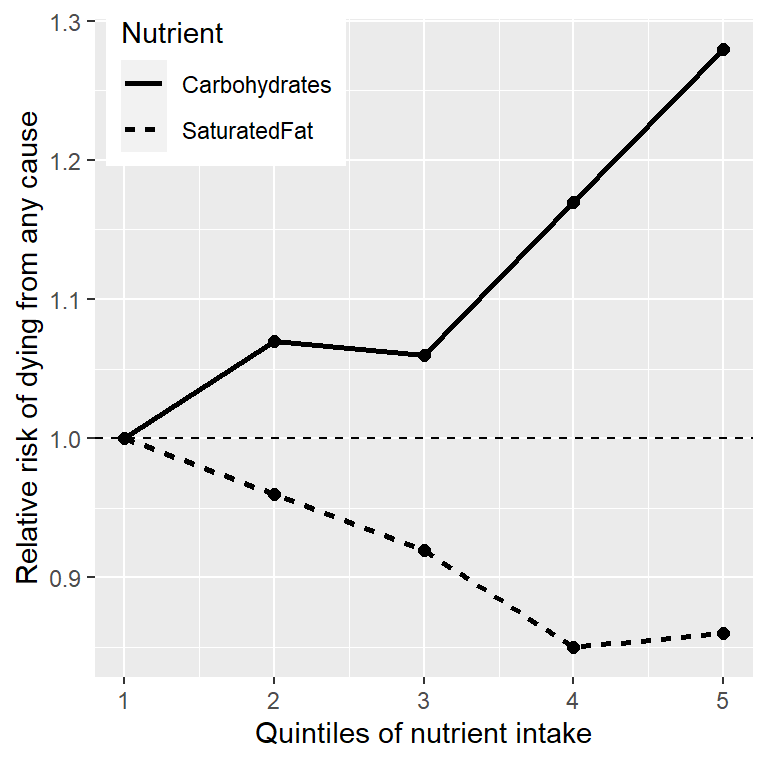
\includegraphics[height=0.5\textheight]{StatsThinking21_files/figure-latex/PureDeathSatFat-1} \caption{Una gráfica de datos del estudio PURE, mostrando la relación entre muerte debido a cualquier causa y la ingesta relativa de grasas saturadas y carbohidratos.}\label{fig:PureDeathSatFat}
\end{figure}

Esta gráfica está basada en diez números. Para obtener estos números, lxs investigadorxs dividieron el grupo de 135,335 participantes (al que llamaremos ``muestra'') en 5 grupos (``quintiles'') después se ordenaron en términos de su ingesta nutrimental; el primer quintil contiene el 20\% de personas con la menor ingesta, y el 5to quintil contiene el 20\% de la mayor ingesta. Lxs investigadorxs luego calcularon qué tan seguido las personas en cada uno de esos grupos había muerto durante el periodo que habían sido estudiadxs. La figura expresa esto en términos del \emph{riesgo relativo} de morir en comparación al quintil menor: Si este número es mayor que uno, significa que las personas en ese grupo son \emph{más} propensas a morir que las personas en el quintil menor, mientras que si es menor que uno, significa que las personas en este grupo son \emph{menos} propensas a morir. La figura es bastante clara: Las personas que comían más grasas saturadas eran \emph{menos} probable de morir durante el estudio, con la menor tasa de muerte vista para personas que estaban en el cuarto quintil (es decir, que comió más grasa que el 60\% más bajo pero menos que el 20\% superior). Lo contrario fue observado en la ingesta de carbohidratos; la mayor cantidad de carbohidratos que una persona comiera, la mayor probabilidad que tenían de morir durante el estudio. Este ejemplo muestra cómo podemos utilizar estadística para \emph{describir} una compleja base de datos en términos mucho más sencillos con un conjunto de números; si tenemos que revisar los datos de cada participante del estudio al mismo tiempo, estaríamos saturadxs con datos y sería más complicado observar el patrón que emerge cuando son descritos de una manera más sencilla.

Los números en la Figura \ref{fig:PureDeathSatFat} parecen mostrar que las muertes disminuyen con la ingesta de grasas saturadas y aumentan con la ingesta de carbohidratos, pero también sabemos que hay mucha incertidumbre en los datos; hay algunas personas que murieron de manera prematura incluso si tenían una dieta baja en carbohidratos, y, de manera similar, algunas personas que comían muchísimos carbohidratos pero vivieron hasta una edad avanzada. Dada esta variabilidad, queremos \emph{decidir} si las relaciones que vemos en los datos son lo sucifiente estrechas como para no esperar que ocurran al azar si no hubiera realmente una relación entre la dieta y la longevidad. La estadística nos provee con las herramientas para tomar este tipo de decisones, y a menudo las personas externas ven esto como el principal y único propósito de la estadística. Pero como veremos a lo largo del libro, esta necesidad de tomar decisiones en blanco y negro basadas en evidencias vagas a menudo ha llevado a los investigadores por mal camino.

Basándonos en los datos, también nos gustaría hacer predicciones sobre resultados futuros. Por ejemplo, es posible que una compañía de seguros de vida desee usar datos sobre la ingesta de grasas y carbohidratos de una persona en particular para predecir cuánto tiempo es probable que viva. Un aspecto importante de la predicción es que requiere que generalicemos a partir de los datos que ya tenemos a alguna otra situación, a menudo en el futuro; si nuestras conclusiones se limitaran a las personas específicas del estudio en un momento determinado, entonces el estudio no sería muy útil. En general, lxs investigadorxs deben asumir que su muestra particular es representativa de una \emph{población} más grande, lo que requiere que obtengan la muestra de una manera que proporcione una imagen no sesgada de la población. Por ejemplo, si el estudio PURE hubiera reclutado a todos sus participantes de sectas religiosas que practican el vegetarianismo, probablemente no querríamos generalizar los resultados a personas que siguen diferentes estándares dietéticos.

\hypertarget{las-grandes-ideas-de-la-estaduxedstica}{%
\section{Las grandes ideas de la estadística}\label{las-grandes-ideas-de-la-estaduxedstica}}

Hay un número de ideas sumamente básicas que interceptan casi todos los aspectos del pensamiento estadístico. Algunas de ellas son señaladas por (\protect\hyperlink{ref-stig}{Stigler 2016}) en su increíble libro ``Los Siete Pilares de la sabiduría Estadística'', el cual he ampliado aquí.

\hypertarget{aprendiendo-de-los-datos}{%
\subsection{Aprendiendo de los datos}\label{aprendiendo-de-los-datos}}

Una forma de pensar en la estadística es como un conjunto de herramientas que nos permiten aprender de los datos. En cualquier situación, comenzamos con un conjunto de ideas o \emph{hipótesis} sobre cuál podría ser el caso. En el estudio PURE, lxs investigadorxs pueden haber comenzado con la expectativa de que comer más grasa conduciría a tasas de mortalidad más altas, dado el dogma negativo predominante sobre las grasas saturadas. Más adelante en el curso presentaremos la idea de \emph{conocimiento previo}, que pretende reflejar el conocimiento que aportamos a una situación. Este conocimiento previo puede variar en su fuerza, a menudo basado en nuestra cantidad de experiencia; si visito un restaurante por primera vez, es probable que tenga una expectativa débil de lo bueno que será, pero si visito un restaurante donde he comido diez veces antes, mis expectativas serán mucho más fuertes. De manera similar, si miro un sitio de reseñas de restaurantes y veo que la calificación promedio de un restaurante de cuatro estrellas se basa solo en tres reseñas, tendré una expectativa más débil de la que tendría si se basara en 300 reseñas.

La estadística nos proporciona una manera de describir cómo se pueden utilizar mejor los nuevos datos para actualizar nuestras creencias y, de esta manera, existen vínculos profundos entre la estadística y la psicología. De hecho, muchas teorías del aprendizaje humano y animal de la psicología están estrechamente alineadas con ideas del nuevo campo del \emph{aprendizaje automático} (\emph{machine learning}). El aprendizaje automático es un campo en la interfaz de las estadísticas y la informática que se centra en cómo construir algoritmos informáticos que puedan aprender de la experiencia. Si bien las estadísticas y el aprendizaje automático a menudo intentan resolver los mismos problemas, los investigadores de estos campos suelen adoptar enfoques muy diferentes; el famoso estadístico Leo Breiman una vez se refirió a ellos como ``Las dos culturas'' para reflejar cuán diferentes pueden ser sus enfoques {[}@ breiman2001{]}. En este libro intentaré combinar las dos culturas porque ambos enfoques proporcionan herramientas útiles para pensar en los datos.

\hypertarget{agregaciuxf3n-aggregation}{%
\subsection{\texorpdfstring{Agregación (\emph{aggregation})}{Agregación (aggregation)}}\label{agregaciuxf3n-aggregation}}

Otra manera de pensar en la estadística es como ``la ciencia de tirar datos''. En el ejemplo anterior del estudio PURE, tomamos más de 100,000 números y los condensamos a diez. Es esta clase de \emph{agregación} la que es uno de los conceptos más importantes de la estadística. Cuando fue desarrollado por primera vez, fue revolucionario: si descartamos todos los detalles sobre cada uno de lxs participantes, ¿cómo podemos estar seguros de que no nos estamos perdiendo algo importante?

Como veremos, la estadística nos proporciona formas de caracterizar la estructura de agregados de datos, y con fundamentos teóricos que explican por qué esto suele funcionar bien. Sin embargo, también es importante tener en cuenta que la agregación puede ir demasiado lejos, y más adelante encontraremos casos en los que un resumen puede proporcionar una imagen engañosa de los datos que se resumen.

\hypertarget{incertidumbre}{%
\subsection{Incertidumbre}\label{incertidumbre}}

El mundo es un lugar incierto. Ahora sabemos que fumar cigarrillos causa cáncer de pulmón, pero esta causa es probabilística: un hombre de 68 años que ha fumado dos paquetes al día durante los últimos 50 años y sigue fumando tiene un riesgo del 15\% (1 de cada 7) de contraer cáncer de pulmón, que es mucho mayor que la probabilidad de cáncer de pulmón en una persona que no fuma. Sin embargo, también significa que habrá muchas personas que fumarán durante toda su vida y nunca tendrán cáncer de pulmón. La estadística nos proporciona las herramientas para caracterizar la incertidumbre, tomar decisiones en condiciones de incertidumbre y realizar predicciones cuya incertidumbre podemos cuantificar.
A menudo se ve a lxs periodistas escribir que lxs investigadorxs científicos han ``probado'' algunas hipótesis. Pero el análisis estadístico nunca puede ``probar'' una hipótesis, en el sentido de demostrar que debe ser verdadera (como se haría en una prueba lógica o matemática). La estadística puede proporcionarnos evidencias, pero siempre son provisionales y están sujetas a la incertidumbre que siempre está presente en el mundo real.

\hypertarget{muestreo-de-una-poblaciuxf3n}{%
\subsection{Muestreo de una población}\label{muestreo-de-una-poblaciuxf3n}}

El concepto de agregación implica que podemos obtener información útil al colapsar los datos, pero ¿cuántos datos necesitamos? La idea de \emph{muestreo} dice que podemos resumir una población completa basándonos en solo una pequeña cantidad de muestras de la población, siempre que esas muestras se obtengan de la manera correcta. Por ejemplo, el estudio PURE inscribió una muestra de aproximadamente 135,000 personas, pero su objetivo era proporcionar información sobre los miles de millones de seres humanos que componen la población de la que se tomaron muestras. Como ya comentamos anteriormente, la forma en que se obtiene la muestra del estudio es fundamental, ya que determina qué tan ampliamente podemos generalizar los resultados. Otra idea fundamental sobre el muestreo es que, si bien las muestras más grandes son siempre mejores (en términos de su capacidad para representar con precisión a toda la población), hay rendimientos decrecientes a medida que la muestra aumenta. De hecho, la velocidad a la que disminuye el beneficio de muestras más grandes sigue una regla matemática simple, que crece como la raíz cuadrada del tamaño de la muestra, de modo que para duplicar la calidad de nuestros datos necesitamos cuadriplicar el tamaño de nuestra muestra.

\hypertarget{causalidad-y-estaduxedstica}{%
\section{Causalidad y estadística}\label{causalidad-y-estaduxedstica}}

El estudio PURE pareció proporcionar pruebas bastante sólidas de una relación positiva entre comer grasas saturadas y vivir más tiempo, pero esto no nos dice lo que realmente queremos saber: si comemos más grasas saturadas, ¿nos hará vivir más tiempo? Esto se debe a que no sabemos si existe una relación causal directa entre comer grasas saturadas y vivir más tiempo. Los datos son consistentes con tal relación, pero son igualmente consistentes con algún otro factor que causa tanto una mayor cantidad de grasas saturadas como una vida más larga. Por ejemplo, es probable que las personas que son más ricas consuman más grasas saturadas y las personas más ricas tienden a vivir más tiempo, pero su vida más larga no se debe necesariamente a la ingesta de grasas, sino que podría deberse a una mejor atención de la salud, una reducción del estrés psicológico, mejor calidad de los alimentos o muchos otros factores. Los investigadores del estudio PURE intentaron tener en cuenta estos factores, pero no podemos estar seguros de que sus esfuerzos eliminaron por completo los efectos de otras variables. El hecho de que otros factores puedan explicar la relación entre la ingesta de grasas saturadas y la muerte es un ejemplo de por qué las clases de introducción a la estadística a menudo enseñan que ``la correlación no implica causalidad'', aunque el renombrado experto en visualización de datos Edward Tufte ha agregado, ``pero seguro que es una pista.''

Aunque la investigación observacional (como el estudio PURE) no puede demostrar de manera concluyente las relaciones causales, generalmente pensamos que la causalidad se puede demostrar utilizando estudios que controlan y manipulan experimentalmente un factor específico. En medicina, este tipo de estudio se conoce como \emph{ensayo controlado aleatorio} (ECA, del inglés \emph{randomized controlled trial}, RCT). Digamos que queríamos hacer un ECA para examinar si el aumento de la ingesta de grasas saturadas aumenta la esperanza de vida. Para hacer esto, tomaríamos muestras de un grupo de personas y luego las asignaríamos a un grupo de tratamiento (al que se le indicaría que aumentara su ingesta de grasas saturadas) o un grupo de control (al que se le diría que siguiera comiendo lo mismo que antes) . Es fundamental que asignemos a los individuos a estos grupos al azar. De lo contrario, las personas que eligen el tratamiento pueden ser diferentes de alguna manera a las personas que eligen el grupo de control; por ejemplo, es más probable que también adopten otros comportamientos saludables. Luego seguiríamos a los participantes a lo largo del tiempo y veríamos cuántas personas de cada grupo murieron. Debido a que asignamos al azar a los participantes a los grupos de tratamiento o de control, podemos estar razonablemente seguros de que no hay otras diferencias entre los grupos que \emph{confundirían} el efecto del tratamiento; sin embargo, todavía no podemos estar seguros porque a veces la aleatorización produce grupos de tratamiento versus grupos de control que \emph{varían} de alguna manera importante. Lxs investigadores a menudo intentan abordar estos factores de confusión mediante análisis estadísticos, pero eliminar la influencia de un factor de confusión de los datos puede resultar muy difícil.

Varios ECA han examinado la cuestión de si cambiar la ingesta de grasas saturadas da como resultado una mejor salud y una vida más larga. Estos ensayos se han centrado en \emph{reducir} las grasas saturadas debido al fuerte dogma entre los investigadores en nutrición de que las grasas saturadas son mortales; la mayoría de estos investigadores probablemente habrían argumentado que no era ético hacer que las personas comieran \emph{más} grasas saturadas. Sin embargo, los ECA han mostrado un patrón muy consistente: en general, no hay un efecto apreciable sobre las tasas de muerte al reducir la ingesta de grasas saturadas.

\hypertarget{objetivos-de-aprendizaje}{%
\section{Objetivos de aprendizaje}\label{objetivos-de-aprendizaje}}

Al leer este capítulo, tu deberías de ser capaz de:

\begin{itemize}
\tightlist
\item
  Describir los objetivos centrales y conceptos fundamentales de la estadística.
\item
  Describir la diferencia entre investigación experimental y observacional con respecto a lo que puede inferir sobre la causalidad.
\item
  Explicar cómo la aleatorización nos provee con la habilidad para hacer inferencias acerca de la causalidad.
\end{itemize}

\hypertarget{lecturas-sugeridas}{%
\section{Lecturas sugeridas}\label{lecturas-sugeridas}}

\begin{itemize}
\tightlist
\item
  \emph{The Seven Pillars of Statistical Wisdom}, by Stephen Stigler
\item
  \emph{The Lady Tasting Tea: How Statistics Revolutionized Science in the Twentieth Century}, by David Salsburg
\item
  \emph{Naked Statistics: Stripping the Dread from the Data}, by Charles Wheelan
\end{itemize}

\hypertarget{trabajar-con-datos}{%
\chapter{Trabajar con Datos}\label{trabajar-con-datos}}

\hypertarget{quuxe9-son-los-datos}{%
\section{¿Qué son los datos?}\label{quuxe9-son-los-datos}}

Cuando hablamos de los datos lo hacemos en plural. Si te encuentras buscando información de estadística en inglés y aparece como ``data'', recuerda que se trata de una palabra que siempre permanece en plural.

\hypertarget{datos-cualitativos}{%
\subsection{Datos Cualitativos}\label{datos-cualitativos}}

Los datos se componen de \emph{variables}, en donde una variable refleja una medida o cantidad única. Algunas variables son \emph{cualitativas}, lo que significa que describen una cualidad en lugar de una cantidad numérica. Por ejemplo, en mi curso de estadística generalmente doy un cuestionario introductorio, con el propósito de obtener datos que pueda usar en clase y para aprender más sobre los estudiantes. Una de las preguntas que hago es ``¿Cuál es tu comida favorita?'', a lo cual algunas de las respuestas han sido: arándanos, chocolate, tamales, pasta, pizza y mango. Esos datos no son esencialmente numéricos; podríamos asignarles números a cada uno (1=arándanos, 2=chocolate, etc), pero solamente estaríamos utilizando los números como etiquetas en lugar de números reales; por ejemplo, no tendría sentido sumar los números en este caso. Sin embargo, a menudo codificaremos datos cualitativos utilizando números para poder trabajar más facilmente con ellos, como verán más adelante en este libro.

\hypertarget{datos-cuantitativos}{%
\subsection{Datos cuantitativos}\label{datos-cuantitativos}}

Más comunmente en estadística trabajaremos con datos \emph{cuantitativos}, lo cual significa que los datos son numéricos. Por ejemplo, aquí en la Tabla \ref{tab:WhyTakingClass} muestra los resultados de otra de las preguntas que realizo en mi clase introductoria, la cual es ``¿Por qué estás tomando esta clase?''

\begin{table}

\caption{\label{tab:WhyTakingClass}Counts of the prevalence of different responses to the question "Why are you taking this class?"}
\centering
\begin{tabular}[t]{lr}
\toprule{}
Why are you taking this class? & Number of students\\
\midrule{}
It fulfills a degree plan requirement & 105\\
It fulfills a General Education Breadth Requirement & 32\\
It is not required but I am interested in the topic & 11\\
Other & 4\\
\bottomrule{}
\end{tabular}
\end{table}

Nota que las respuestas de los estudiantes fueron cualitativas, pero generamos un resumen cuantitativo de ellos contando cuántos estudiantes respondieron a cada opción.

\hypertarget{tipos-de-nuxfameros}{%
\subsection{Tipos de números}\label{tipos-de-nuxfameros}}

Existen varios tipos diferentes de números con los que trabajamos en estadística. Es importante entender estas diferencias, en parte porque los lenguajes de programación como R a menudo los distinguen.

\textbf{Números binarios}. Los más simples son los números binarios -- cero ó uno. A menudo usaremos números binarios para representar si algo es verdadero o falso, o presente o ausente. Por ejemplo, puede que le pregunte a 10 personas si alguna vez han tenido dolor de cabeza por migraña, registrando sus respuestas como ``Sí'' ó ``No''. En ocasiones es útil usar valores \emph{lógicos}, los cuales toman los valores de \texttt{VERDADERO} o \texttt{FALSO}. Esto puede ser especialmente útil cuando comenzamos a utilizar lenguajes de programación como R para analizar nuestros datos, ya que, estos lenguajes comprenden los conceptos de VERDADERO y FALSO. De hecho, la mayoría de los lenguajes de programación tratan los valores de verdad y los números binarios de manera equivalente. El número 1 es igual al valor lógico \texttt{VERDADERO}, y el número cero es igual al valor lógico \texttt{FALSO}.

\textbf{Enteros}. Los enteros son números enteros sin fracción o punto decimal. Nos encontramos más comunmente números enteros cuando contamos cosas, pero también ocurren en la medición de aspectos psicológicos. Por ejemplo, en mi cuestionario introductorio administro un set de preguntas sobre actitudes hacia la estadística (tal como ``La estadística me parece misteriosa.''), para lo cual les estudiantes responden con un número entre 1 (``Muy en desacuerdo'') y 7 (``Muy de acuerdo'').

\textbf{Números reales}. En estadística trabajamos más comunmente con números reales, los cuales tienen parte fraccionaria o decimal. Por ejemplo, cuando medimos el peso de alguien, éste puede ser medido a un nivel arbitrario de precisión, desde kilogramos hasta microgramos.

\hypertarget{mediciones-discretas-versus-continuas}{%
\section{Mediciones Discretas versus Continuas}\label{mediciones-discretas-versus-continuas}}

Una medición \emph{discreta} es aquella que toma uno de un conjunto de valores particulares. Estos pueden ser valores cualitativos (por ejemplo, diferentes tipos de razas de perros) o valores numéricos (por ejemplo, cuántos amigos tiene une en facebook). Es importante recordar que, no hay punto medio en las medidas; no tiene sentido decir que une tiene 33.7 amigues.

Una medición \emph{continua} es aquella que es definida en términos de un número real. Puede encontrarse en cualquier parte de un rango particular de valores, aunque usualmente nuestras herramientas de medición pueden limitar la precisión con la que podemos medirla; por ejemplo, una báscula de piso puede medir el peso al kilogramo más cercano, aunque en teoría el peso puede ser medido con mucha mayor precisión.

En los cursos de estadística es común revisar con más detalle las diferentes ``escalas'' de medición, las cuales son discutidas con más detalle en el Apéndice de este capítulo. El punto más importante a recordar de esto es que algunos tipos de estadística no hacen sentido con algunos tipos de datos. Por ejemplo, imagina que reunieramos el código postal de un grupo de individuos. Esos números son representados como enteros, pero en realidad no se refieren a una escala numérica; cada código postal sirve básicamente como etiqueta para una región diferente. Por esta razón, no tendría sentido hablar del código postal promedio.

\hypertarget{quuxe9-constituye-a-una-buena-mediciuxf3n}{%
\section{¿Qué constituye a una buena medición?}\label{quuxe9-constituye-a-una-buena-mediciuxf3n}}

En muchas áreas, como en la psicología, aquello que estamos midiendo no es una característica física, sino más bien un concepto teórico inobservable, a lo cual usualmente nos referimos como un \emph{constructo}. Por ejemplo, digamos que quiero probar qué tan bien entiendes la distinción entre los diferentes tipos de números descritos anteriormente. Te podría dar un examen sorpresa en donde te haría varias preguntas sobre estos conceptos y contaría cuántas respuestas tienes correctas. Esta prueba puede o puede no ser una buena medición del constructo de tu conocimiento real-- por ejemplo, si escribiera una prueba en una forma confusa o un lenguaje que tú no entiendes, entonces la prueba puede sugerir que no entiendes los conceptos cuando en realidad sí los entiendes. Por otro lado, si te doy una prueba de opción múltiple con muchas respuestas obviamente incorrectas, entonces es posible que puedas desempeñarte bien en la prueba, incluso si en realidad no comprendes el material.

Usualmente es imposible medir un constructo sin cierto margen de error. En el ejemplo de arriba, puede que sepas la respuesta, pero puede que hayas leído mal la pregunta y por ende, obtenido una respuesta incorrecta. En otros casos, puede haber errores intrínsecos con respecto a aquella cosa que quiere ser medida, como cuando medimos cuánto le toma a una persona reaccionar en una simple prueba de tiempo de reacción, las cuales pueden variar de prueba en prueba por muchas razones. Generalmente queremos que nuestro error de medición sea lo más bajo posible.

A veces existe un estándar con el que se pueden probar otras mediciones, al que podríamos referirnos como un ``estándar dorado'' -- por ejemplo, la medición del sueño se puede realizar utilizando muchos dispositivos diferentes (como dispositivos que miden el movimiento de una persona mientras duerme), pero generalmente se consideran inferiores al estandar dorado de la polisomnografía (el cual es un examen que mide ondas cerebrales para cuantificar la cantidad de tiempo que una persona pasa en cada etapa del sueño). A menudo, el estandar dorado es más difícil o más caro de utilizar, y el método más barato es usado incluso cuando pueda tener un mayor margen de error.

Cuando pensamos en aquello que constituye a una buena medición, usualmente distinguimos dos diferentes aspectos que debe tener: debe de ser \emph{confiable}, y debe de ser \emph{válida}.

\hypertarget{confiabilidad}{%
\subsection{Confiabilidad}\label{confiabilidad}}

La confiabilidad se refiere a la consistencia de nuestras mediciones. Una forma común de confiabilidad, conocida como ``confiabilidad test-retest'', mide qué tan bien concuerdan las mediciones si la misma medición se realiza dos veces. Por ejemplo, si te doy un cuestionario sobre tu actitud con respecto a la estadística hoy, y repito este mismo cuestionario mañana, al comparar tus respuestas en los dos días esperaríamos que tuvieran resultados muy similares entre sí, a menos que algo sucediera entre la aplicación de ambos cuestionarios que haya cambiado tu perspectiva de la estadística (¡como leer este libro!).

Otra forma de evaluar la confiabilidad surge en casos en que los datos incluyen juicios subjetivos. Por ejemplo, digamos que unx investigadorx quiere determinar si un tratamiento cambia qué tan bien interactúa unx niñx que se encuentra dentro del espectro autista con otros niñxs, lo cual es medido a través de expertos que observan al niñx y califican sus interacciones con lxs otrxs niñxs. En este caso queremos asegurarnos de que las respuestas no dependan del individuo que está calificando-- nos gustaría que existiera una alta \emph{confiabilidad entre calificadores}. Esto puede ser evaluado teniendo más de unx solx evaluadorx, y después al comparar sus calificaciones asegurarnos de que concuerden entre sí.

La confiabilidad es importante si queremos comparar una medición con otra. La relación entre dos variables diferentes no puede ser más fuerte que la relación entre cualquiera de las variables y ella misma (es decir, su confiabilidad). Esto significa que una medición no confiable nunca puede tener una relación estadísticamente fuerte con cualquier otra medición. Por esta razón, lxs investigadorxs que desarrollan una nueva medición (como un nuevo cuestionario) a menudo realizarán todo lo posible para establecer y mejorar su confiabilidad.

\begin{figure}
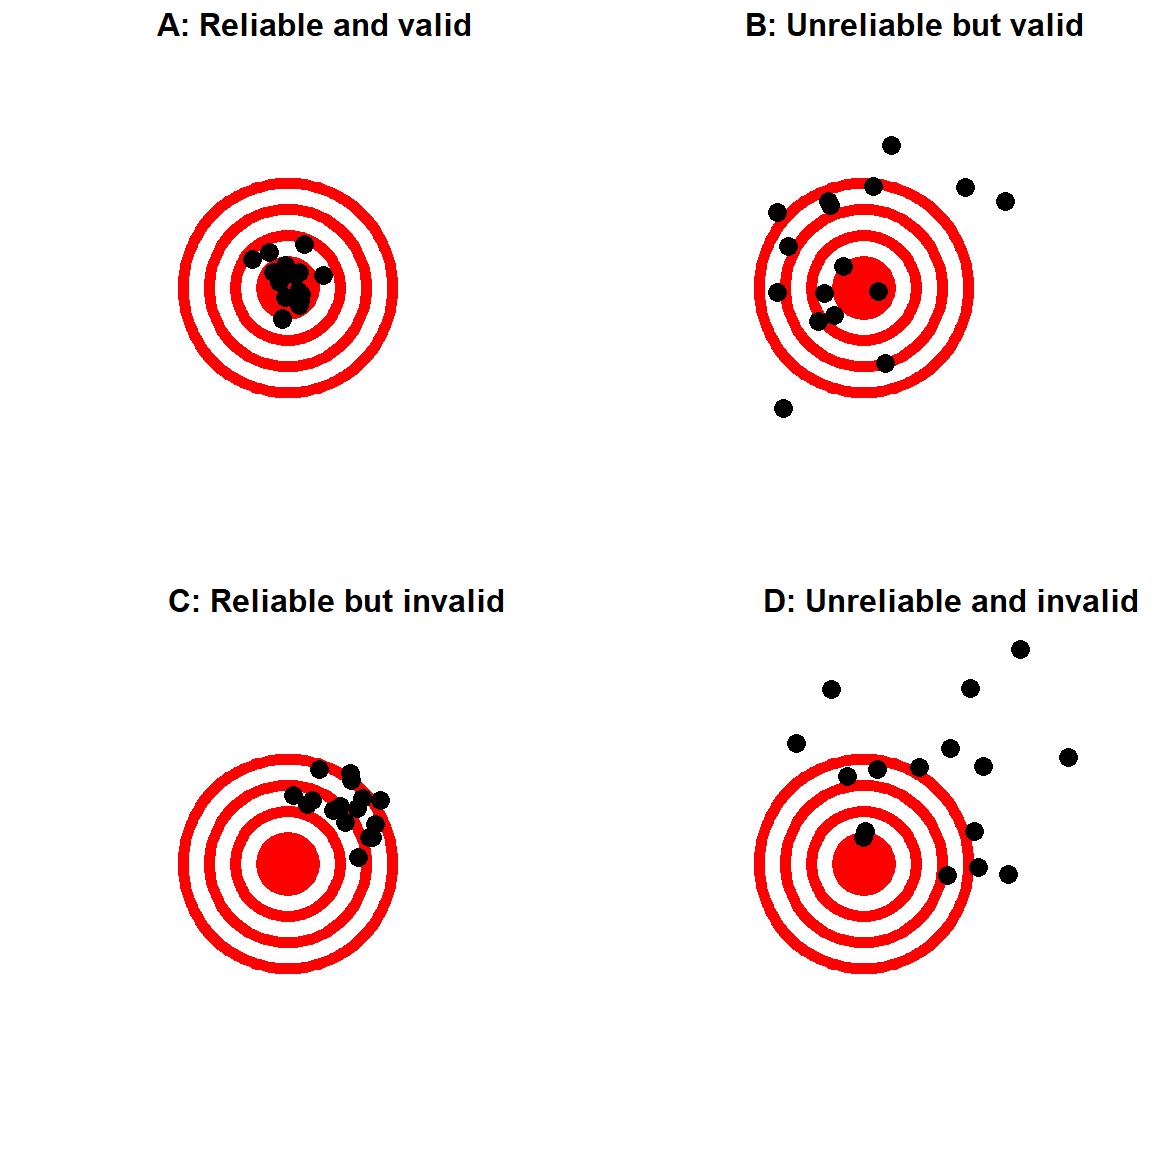
\includegraphics[height=0.33\textheight]{StatsThinking21_files/figure-latex/ReliabilityValidity-1} \caption{A figure demonstrating the distinction between reliability and validity, using shots at a bullseye. Reliability refers to the consistency of location of shots, and validity refers to the accuracy of the shots with respect to the center of the bullseye. }\label{fig:ReliabilityValidity}
\end{figure}

\hypertarget{validez}{%
\subsection{Validez}\label{validez}}

La confiabilidad es importante, pero por sí misma no es suficiente: Después de todo, todo lo que pueda crear mediciones perfectamente confiables en una prueba de personalidad a través de re-codificar todas las respuestas utilizando el mismo número, a pesar de cómo responda la persona. Queremos que nuestras mediciones sean también \emph{válidas}-- esto quiere decir que, nos queremos asegurar de que en realidad estemos midiendo el constructo que pensamos que estamos midiendo (Figura \ref{fig:ReliabilityValidity}). Existen varios tipos diferentes de validez que son comúnmente discutidos; a continuación nos enfocaremos en tres de ellos.

\emph{Validez aparente}. ¿La medición tiene sentido de forma aparente? Si te dijera que voy a medir la presión sanguínea de una persona con sólo observar el color de su lengua, probablemente pensarías que esta no es una medición válida aparente. Por otro lado, al utilizar un brazalete para medir la presión sanguínea tiene validez aparente. Esto es solamente un ejemplo simple antes de que nos centremos en aspectos más complejos de la validez.

\emph{Validez de constructo}. Primero hay que preguntarnos, ¿es esta medición relacionada con otras mediciones de una forma apropiada? A menudo esto se subdivide en dos aspectos. \emph{Validez convergente} quiere decir que la medición debería de estar estrechamente relacionada con otras mediciones que se supone reflejan el mismo constructo. Digamos que me interesa medir qué tan extrovertida es una persona mediante un cuestionario o una entrevista. La validez convergente se demostraría si estas dos medidas diferentes estuvieran estrechamente relacionadas entre sí. Por otro lado, las mediciones que se cree que reflejan diferentes constructos no deben estar relacionadas, lo que se conoce como \emph{validez divergente}. Si mi teoría de la personalidad dice que la extraversión y la responsabilidad son dos constructos distintos, entonces también debería poder observar que mi medición de la extraversión \emph{no está relacionada} con la medición de la responsabilidad.

\emph{Validez predictiva} Si nuestras mediciones son verdaderamente válidas, entonces también deberían de poder predecir otros resultados. Por ejemplo, digamos que pensamos que el rasgo psicológico de la búsqueda de sensaciones (el deseo de nuevas experiencias) está relacionado con la toma de riesgos en el mundo real. Para probar la validez predictiva de una medición de la búsqueda de sensaciones, probaríamos qué tan bien los puntajes en la prueba predicen los puntajes en un cuestionario diferente que mide la toma de riesgos en el mundo real.

\hypertarget{objetivos-de-aprendizaje-1}{%
\section{Objetivos de aprendizaje}\label{objetivos-de-aprendizaje-1}}

Al haber leído este capítulo deberías de ser capaz de:

\begin{itemize}
\tightlist
\item
  Distinguir entre diferentes tipos de variables (cuantitativas/cualitativas, binarios/enteros/reales, discretos/continuos) y poder dar ejemplos de cada una de estas variables.
\item
  Distinguir entre conceptos de confiabilidad y validez y poder aplicar cada concepto a un conjunto de datos en particular.
\end{itemize}

\hypertarget{lecturas-sugeridas-1}{%
\section{Lecturas sugeridas}\label{lecturas-sugeridas-1}}

\begin{itemize}
\tightlist
\item
  \href{http://www.personality-project.org/r/book/}{\emph{An Introduction to Psychometric Theory with Applications in R}} - A free online textbook on psychological measurement
\end{itemize}

\hypertarget{apuxe9ndice}{%
\section{Apéndice}\label{apuxe9ndice}}

\hypertarget{escalas-de-mediciuxf3n}{%
\subsection{Escalas de medición}\label{escalas-de-mediciuxf3n}}

Todas las variables deben tomar al menos dos valores diferentes posibles (de lo contrario, serían una \emph{constante} en lugar de una variable), pero diferentes valores de la variable pueden relacionarse entre sí de diferentes maneras, a estas nos referimos como \emph{escalas de medición}. Hay cuatro formas en las que pueden diferir los diferentes valores de una variable.

\begin{itemize}
\tightlist
\item
  \emph{Identidad}: Cada valor de la variable tiene un significado único.
\item
  \emph{Magnitud}: Los valores de la variable reflejan diferentes magnitudes y tienen una relación ordenada entre sí-- por lo tanto, algunos valores son mayores y otros son menores.
\item
  \emph{Intervalos iguales}: Las unidades a lo largo de la escala de medición son iguales entre sí. Esto quiere decir, por ejemplo, que la diferencia entre 1 y 2 sería igual en su magnitud a la diferencia entre 19 y 20.
\item
  \emph{Cero absoluto}: La escala tiene un verdadero punto cero significativo. Por ejemplo, para muchas mediciones de cantidades físicas como la altura o el peso, esta es la ausencia total de la cosa que está siendo medida.
\end{itemize}

Hay cuatro escalas diferentes de medición que van de la mano con estas diferentes formas en que los valores de una variable pueden diferir.

\emph{Escala Nominal}. Una variable nominal satisface el criterio de identidad, de modo que cada valor de la variable representa algo diferente, pero los números simplemente sirven como etiquetas cualitativas, como mencionamos al principio. Por ejemplo, es posible que le preguntemos a las personas el partido politico al que se suscriben, y después codificar esa información como números: 1= ``Republicanos'', 2= ``Demócrata'', 3= ``Libertaria'', etc. Sin embargo, los números no tienen ninguna relación ordenada entre sí.

\emph{Escala ordinal}. Una variable ordinal satisface el criterio de identidad y magnitud, como que el valor puede ser ordenado en términos de su magnitud. Por ejemplo, le podemos preguntar a una persona con dolor crónico que llene un formato diario en donde evalúe qué tan mal siente su dolor, utilizando una escala numérica del 1 al 7. Hay que tomar en cuenta que, si bien la persona presumiblemente siente más dolor en un día en el que reporta un 6 frente a un día en que reporta un 3, no tendría sentido decir que su dolor es dos veces más intenso en el primero que en el último día; el orden nos da información sobre la magnitud relativa, pero las diferencias entre los valores no son necesariamente iguales en magnitud.

\emph{Escala de Intervalo}. Una escala de intervalo tiene todas las características de una escala ordinal, pero además los intervalos entre unidades en la escala de medición pueden tratarse como iguales. Un ejemplo estándar es la temperatura física medida en grados Celsius o Fahrenheit; la diferencia física entre 10 y 20 grados es la misma que la diferencia física entre 90 y 100 grados, pero cada escala también puede tomar valores negativos.

\emph{Escala de proporción (o de razón)}. Una variable a escala de proporción/razón tiene las cuatro características que se describen anteriormente: Identidad, magnitud, intervalos iguales y cero absoluto. La diferencia entre una variable de escala de razón y una variable de escala de intervalo es que la variable de escala de razón tiene un verdadero punto cero. Ejemplos de variables de escala de razón incluyen la altura y el peso físicos, junto con la temperatura medida en Kelvin.

Hay dos razones importantes a las cuales les debemos de prestar atención a la escala de medición de la variable. En primer lugar, la escala determina qué tipo de operaciones matemáticas podemos aplicar a los datos (see Table \ref{tab:MeasurementTypes}). Una variable nominal solamente se puede comparar por igualdad; es decir, ¿dos observaciones de esa variable tienen el mismo valor numérico? No tendría sentido aplicar otras operaciones matemáticas a una variable nominal, ya que en realidad no funcionan como números en una variable nominal, sino más bien como etiquetas. Con las variables ordinales, también podemos probar si un valor es mayor o menor que otro, pero no podemos hacer ninguna aritmética. Las variables de intervalo y razón nos permiten realizar operaciones aritméticas; con variables de intervalo solo podemos sumar o restar valores, mientras que con variables de razón también podemos multiplicar y dividir valores.

\begin{table}

\caption{\label{tab:MeasurementTypes}Different scales of measurement admit different types of numeric operations}
\centering
\begin{tabular}[t]{lllll}
\toprule{}
  & Equal/not equal & >/< & +/- & Multiply/divide\\
\midrule{}
Nominal & OK &  &  & \\
Ordinal & OK & OK &  & \\
Interval & OK & OK & OK & \\
Ratio & OK & OK & OK & OK\\
\bottomrule{}
\end{tabular}
\end{table}

Estas restricciones también implican que existen ciertos tipos de estadística que podemos calcular sobre cada tipo de variable. La estadística que solamente se trate de contar los diferentes valores (como el valor más común comunido como \emph{modo}), puede ser calculado en cualquiera de los tipos de variables. Otro tipo de estadística está basada en ordenar o en clasificar los valores (como la \emph{mediana}, la cual es el valor que está en medio cuando todos los valores son ordenados por su magnitud), y estos requieren que el valor al menos esté en una escala ordinal. Finalmente, la estadística que se encarga de sumar los valores (como el promedio o \emph{media}), requiere que las variables sean al menos en una escala de intervalo. Habiendo dicho esto, debemos tomar en cuenta que es común que lxs investigadorxs calculen la media de variables que son solo ordinales (como las respuestas en las pruebas de personalidad), pero esto a veces puede ser problemático.

\hypertarget{resumir-datos}{%
\chapter{Resumir datos}\label{resumir-datos}}

Mencioné en la Introducción que uno de los grandes descubrimientos de la estadística es la idea de que podemos entender mejor el mundo si nos deshacemos de información, y eso es justo lo que hacemos cuando resumimos un cojunto de datos.
En este Capítulo discutiremos por qué y cómo resumir datos.

\hypertarget{por-quuxe9-resumir-datos}{%
\section{¿Por qué resumir datos?}\label{por-quuxe9-resumir-datos}}

Cuando resumimos datos, estamos necesariamente tirando información, y uno podría objetar esto plausiblemente. Como un ejemplo, regresemos al estudio PURE que discutimos en el Capítulo 1. ¿No deberíamos pensar que todos los detalles de cada individuo importan, más allá de los que se resumieron en el conjunto de datos? ¿Qué decir de los detalles específicos sobre cómo fue recolectada la información, como el momento del día o el estado de ánimo del participante? Todos esos detalles se pierden cuando resumimos los datos.

Resumimos datos en general porque nos provee de una manera de \emph{generalizar} - esto es, hacer enunciados generales que van más allá de observaciones específicas. La importancia de la generalización fue subrayada por el escritor Jorge Luis Borges en su cuento ``Funes El Memorioso'', donde describe a un individuo que pierde la habilidad de olvidar. Borges se enfoca en la relación entre generalización (i.e.~tirar datos) y el pensamiento: ``Pensar es olvidar diferencias, es generalizar, abstraer. En el abarrotado mundo de Funes no había sino detalles, casi inmediatos''.

Les psicólogues han estudiado por largo tiempo todas las maneras en que la generalización es central al pensamiento. Un ejemplo es la categorización: somos capaces de reconocer fácilmente diferentes ejemplos de la categoría de ``aves'' a pesar de que los ejemplos individuales puedan ser muy diferentes en características superficiales (como un avestruz, un petirrojo, y una gallina). De manera importante, la generalización nos permite hacer predicciones acerca de estos individuos -- en el caso de las aves, podemos predecir que vuelan y comen semillas, y que probablemente no puedan manejar un carro o hablar inglés. Estas predicciones no serán siempre correctas, pero frecuentemente serán suficientemente buenas para ser útiles en el mundo.

\hypertarget{resumiendo-datos-usando-tablas}{%
\section{Resumiendo datos usando tablas}\label{resumiendo-datos-usando-tablas}}

Una manera simple de resumir datos es el generar una tabla que represente el conteo de varios tipos de observaciones. Este tipo de tabla ha sido usado durante miles de años (ve la Figura \ref{fig:salesContract}).

\begin{figure}

\includegraphics[height=0.3\textheight]{images/Sales_contract_Shuruppak_Louvre_AO3760} \caption{Una tabla sumeria en el Louvre, que muestra un contrato de venta de una casa y un terreno. Dominio público, via Wikimedia Commons.}\label{fig:salesContract}
\end{figure}

Veamos algunos ejemplos del uso de tablas, usando un conjunto de datos más realista. A lo largo de este libro usaremos la base de datos de la \href{https://www.cdc.gov/nchs/nhanes/index.htm}{Encuesta Nacional de Nutrición y Salud (National Health and Nutrition Examination Survey, NHANES)}. Este es un estudio en curso que evalúa el status de salud y nutrición de una muestra de individuos de los Estados Unidos en múltiples variables diferentes. Aquí usaremos una versión de la base de datos que está disponible con las librerías del software R. Para este ejemplo, miraremos una variable simple llamada ``PhysActive'' en la base de datos. Esta variable contiene uno de tres diferentes valores: ``Sí'' o ``No'' (indicando si la persona reportó o no el hacer ``deportes moderados o de intensidad vigorosa, actividades de fitness o recreacionales''), o ``NA'' si el dato está perdido para ese individuo. Existen varias razones por las cuales el dato podría estar perdido; por ejemplo, esta pregunta no se le realizó a niños menores a 12 años, mientras que en otros casos un adulto podría haber declinado el contestar la pregunta durante la entrevista.

\hypertarget{frequency-distributions}{%
\subsection{Distribuciones de frecuencias}\label{frequency-distributions}}

Veamos cuántas personas caen en cada una de las categorías:

\begin{tabular}{l|r}
\hline
PhysActive & AbsoluteFrequency\\
\hline
No & 2473\\
\hline
Yes & 2972\\
\hline
NA & 1334\\
\hline
\end{tabular}

Esta tabla muestra las frecuencias de cada uno de los diferentes valores; había 2473 individuos que respondieron ``No'' a la pregunta, 2972 que respondieron ``Sí'', y 1334 de quienes no hubo una respuesta. Llamamos a esto una \emph{distribución de frecuencias} porque nos dice qué tan frecuente sucede en nuestra muestra cada uno de los valores posibles.

Esto nos muestra la frecuencia absoluta de las dos respuestas, para todas las personas que sí dieron una respuesta. De esta información, podemos ver que hubo más personas respondiendo ``Sí'' que ``No'', pero puede ser difícil ver qué tan grande es la diferencia sólo viendo estos números absolutos. Por esta razón, frecuentemente preferimos presentar los datos usando \emph{frecuencias relativas}, que se obtienen dividiendo cada frecuencia entre la suma de todas las frecuencias absolutas:

\[
frecuencia\ relativa_i = \frac{frecuencia\ absoluta_i}{\sum_{j=1}^N frecuencia\ absoluta_j}
\]
La frecuencia relativa provee una manera mucho más fácil para observar qué tan grande es la diferencia. También podemos interpretar las frecuencias relativas como porcentajes si las multiplicamos por 100. En este ejemplo, quitaremos los valores NA, porque nos gustaría poder interpretar las frecuencias relativas de las personas físicamente activas versus las inactivas.

\begin{table}

\caption{\label{tab:unnamed-chunk-5}Frecuencias absolutas y relativas, y porcentajes de la variable PhysActive}
\centering
\begin{tabular}[t]{l|r|r|r}
\hline
PhysActive & AbsoluteFrequency & RelativeFrequency & Percentage\\
\hline
No & 2473 & 0.45 & 45\\
\hline
Yes & 2972 & 0.55 & 55\\
\hline
\end{tabular}
\end{table}

Esto nos deja ver que el 45.4 por ciento de los individuos en la muestra NHANES dijo ``No'' y el 54.6 por ciento dijo ``Sí''.

\hypertarget{cumulative-distributions}{%
\subsection{Distribuciones acumuladas}\label{cumulative-distributions}}

La variable PhysActive que revisamos arriba sólo tenía dos valores posibles, pero frecuentemente queremos resumir datos que pueden tener más valores posibles. Cuando esos valores son cuantitativos, entonces una manera útil de resumirlos es a través de lo que llamamos una representación de frecuencias \emph{acumuladas}: en lugar de preguntarnos cuántas observaciones toman un valor específico, nos preguntamos cuántas observaciones tienen \emph{como máximo} un valor en específico.

Démosle un vistazo a otra variable en la base de datos NHANES, llamada SleepHrsNight que registra cuántas horas el participante reportó que duerme usualmente entre semana. Construyamos una tabla de frecuencias como la que hicimos arriba, después de quitar a las personas que tienen dato perdido en este pregunta.

\begin{table}

\caption{\label{tab:unnamed-chunk-7}Distribución de frecuencias del número de horas de sueño por noche en la base de datos NHANES}
\centering
\begin{tabular}[t]{r|r|r|r}
\hline
SleepHrsNight & AbsoluteFrequency & RelativeFrequency & Percentage\\
\hline
2 & 9 & 0.00 & 0.18\\
\hline
3 & 49 & 0.01 & 0.97\\
\hline
4 & 200 & 0.04 & 3.97\\
\hline
5 & 406 & 0.08 & 8.06\\
\hline
6 & 1172 & 0.23 & 23.28\\
\hline
7 & 1394 & 0.28 & 27.69\\
\hline
8 & 1405 & 0.28 & 27.90\\
\hline
9 & 271 & 0.05 & 5.38\\
\hline
10 & 97 & 0.02 & 1.93\\
\hline
11 & 15 & 0.00 & 0.30\\
\hline
12 & 17 & 0.00 & 0.34\\
\hline
\end{tabular}
\end{table}

Desde este momento podemos resumir los datos sólo al observar la tabla; por ejemplo, podemos ver que la mayoría de las personas reportaron dormir entre 6 y 8 horas. Grafiquemos los datos para ver esto de manera más clara. Para hacer esto podemos graficar un \emph{histograma} que nos permite ver el número de casos que hay por cada uno de los valores; ve el panel izquierdo de la Figura \ref{fig:sleepHist}. También podemos graficar las frecuencias relativas, a este tipo de gráfica nos referirimos frecuentemente como \emph{densidades} - ve el panel derecho de la Figura \ref{fig:sleepHist}.

\begin{figure}
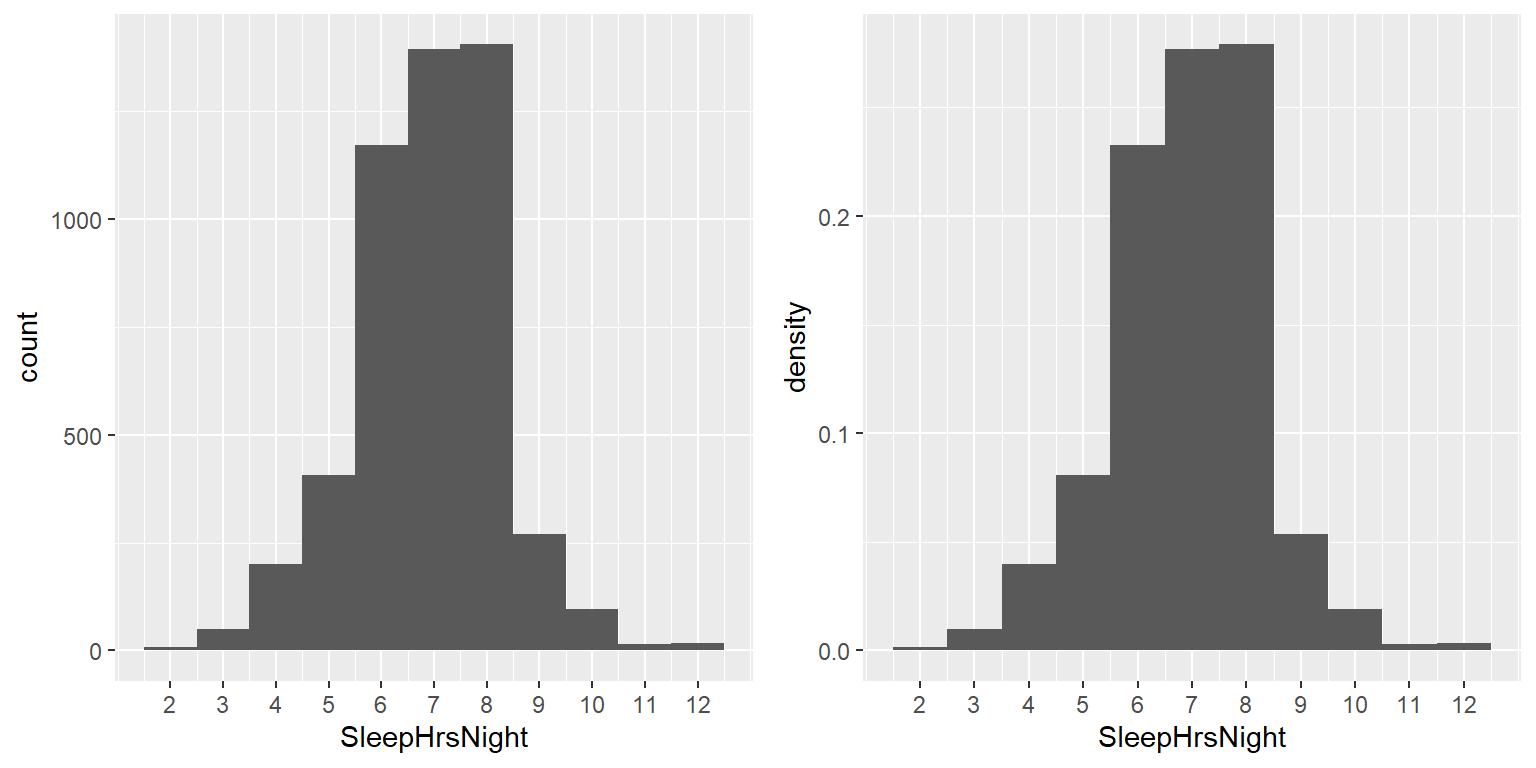
\includegraphics[height=0.33\textheight]{StatsThinking21_files/figure-latex/sleepHist-1} \caption{Histogramas que muestran el número (izquierda) y la proporción (derecha) de las personas que reportaron cada valor posible en la variable SleepHrsNight.}\label{fig:sleepHist}
\end{figure}

¿Qué pasa si quisiéramos saber cuántas personas reportaron dormir 5 horas o menos? Para encontrar esto, podemos calcular una \emph{distribución acumulada}. Para calcular la frecuencia acumulada para un valor j, sumamos las frecuencias de todos los valores hasta j, incluyendo también la frecuencia del valor j:

\[
frecuencia\ acumulada_j = \sum_{i=1}^{j}{frecuencia\ absoluta_i}
\]
Hagamos esto para nuestra variable de sueño, calculemos las frecuencias absolutas y acumuladas en R:

\newpage

\begin{table}

\caption{\label{tab:unnamed-chunk-9}Distribuciones de frecuencias absolutas y acumuladas para la variable SleepHrsNight}
\centering
\begin{tabular}[t]{r|r|r}
\hline
SleepHrsNight & AbsoluteFrequency & CumulativeFrequency\\
\hline
2 & 9 & 9\\
\hline
3 & 49 & 58\\
\hline
4 & 200 & 258\\
\hline
5 & 406 & 664\\
\hline
6 & 1172 & 1836\\
\hline
7 & 1394 & 3230\\
\hline
8 & 1405 & 4635\\
\hline
9 & 271 & 4906\\
\hline
10 & 97 & 5003\\
\hline
11 & 15 & 5018\\
\hline
12 & 17 & 5035\\
\hline
\end{tabular}
\end{table}

En el panel izquierdo de la Figura \ref{fig:sleepAbsCumulRelFreq} graficamos los datos para ver cómo se ven estas representaciones; los valores de frecuencias absolutas están graficados con líneas sólidas (continuas), y las frecuencias acumuladas están graficadas con líneas punteadas. Podemos ver que las frecuencias acumuladas van \emph{incrementándose monotónicamente} -- esto es, sólo pueden ir hacia arriba o mantenerse constantes, pero nunca pueden disminuir. De nuevo, usualmente encontramos las frecuencias relativas más útiles que las absolutas; esas están graficadas en el panel derecho de la Figura \ref{fig:sleepAbsCumulRelFreq}.

\begin{figure}
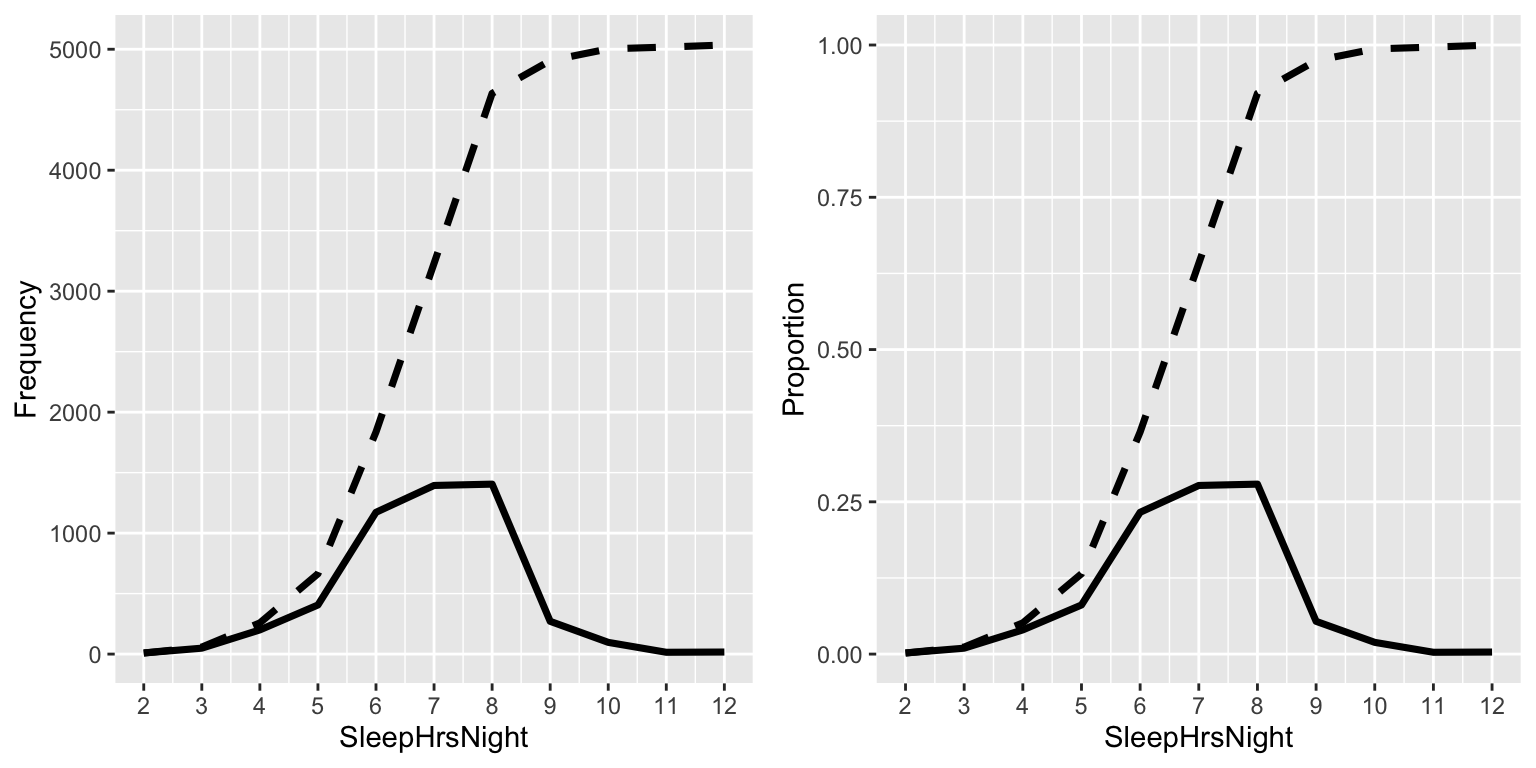
\includegraphics[height=0.33\textheight]{StatsThinking21_files/figure-latex/sleepAbsCumulRelFreq-1} \caption{Gráfica con los valores relativos (líneas sólidas/continuas) y relativos acumulados (líneas punteadas) de las frecuencias (izquierda) y proporciones (derecha) de los posibles valores de SleepHrsNight.}\label{fig:sleepAbsCumulRelFreq}
\end{figure}

\hypertarget{plotting-histograms}{%
\subsection{Graficar histogramas}\label{plotting-histograms}}

\begin{figure}
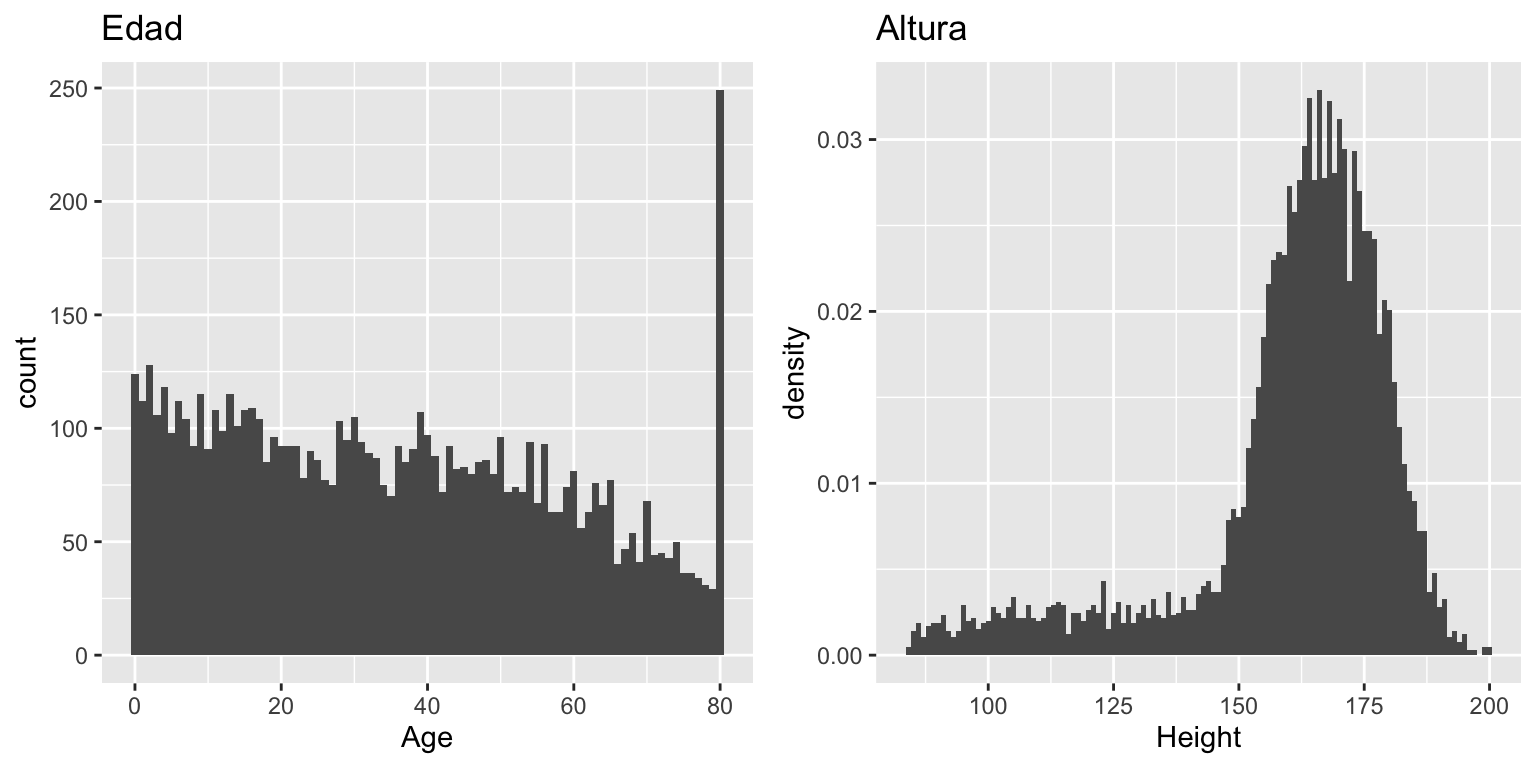
\includegraphics[height=0.33\textheight]{StatsThinking21_files/figure-latex/ageHist-1} \caption{Histograma de las variables de Edad (izquierda) y Altura (derecha) en NHANES.}\label{fig:ageHist}
\end{figure}

Las variables que hemos examinado arriba eran bastante simples, pudiendo tener sólo unos pocos valores posibles. Ahora veamos una variable más compleja: Edad. Primero, grafiquemos la variable Edad para todos los individuos en la base de datos de NHANES (ve el panel izquierdo de la Figura \ref{fig:ageHist}). ¿Qué ves ahí? Primero, deberías notar que el número de individuos en cada grupo de edad va disminuyendo con el tiempo. Esto tiene sentido porque la población fue muestreada aleatoriamente, y pasa que los fallecimientos a lo largo del tiempo lleva a que haya menos personas en los rangos de edad más avanzada. Segundo, probablemente notes un pico grande en la gráfica en la edad de 80 años. ¿Qué piensas que sea eso?

Si buscáramos la información acerca de la base de datos NHANES en R, veríamos la siguiente definición: ``Edad en años del participante al momento de su inclusión en la investigación. Nota: Participantes de 80 años o más fueron registrados como 80.'' La razón para esto es que la muestra relativamente pequeña de individuos con edades muy altas podría hacer potencialmente más fácil el poder identificar a las personas específicas en la base de datos si uno conoce su edad exacta; los investigadores generalmente prometen a sus participantes el mantener su identidad de manera confidencial, y esta es una de las cosas que se pueden hacer para ayudar a proteger a los participantes. Esto subraya el hecho de que siempre es importante conocer de dónde proviene la información que tenemos y conocer cómo ha sido procesada; de otra manera podríamos interpretar los datos de manera inapropiada, pensando que las personas de 80 años de edad hayan sido sobrerrepresentadas en la muestra de alguna manera.

Veamos otra variable más compleja en la base de datos NHANES: Altura. El histograma de los valores de altura está graficada en el panel derecho de la Figura \ref{fig:ageHist}. La primera cosa que deberías notar acerca de esta distribución es que la mayoría de su densidad está centrada alrededor de 170 cm, pero su distribución tiene una ``cola'' a la izquierda; hay un número pequeño de individuos con alturas más pequeñas. ¿Qué piensas que está sucediendo ahí?

Habrás intuido que las alturas pequeñas vienen de niños y niñas en la base de datos. Una manera de examinar esto es graficando un histograma con los colores separados para niños y adultos (panel izquierdo de la Figura \ref{fig:heightHistSep}). Esto muestra que todas las alturas más bajas en efecto son de niños y niñas en la muestra. Realicemos una nueva versión de NHANES que sólo incluya adultos, y después grafiquemos el histograma sólo para ellos (panel derecho de la Figura \ref{fig:heightHistSep}). En esa gráfica la distribución se mira mucho más simétrica. Como veremos después, este es un buen ejemplo de una distribución \emph{normal} (o \emph{Gaussiana}).

\begin{figure}
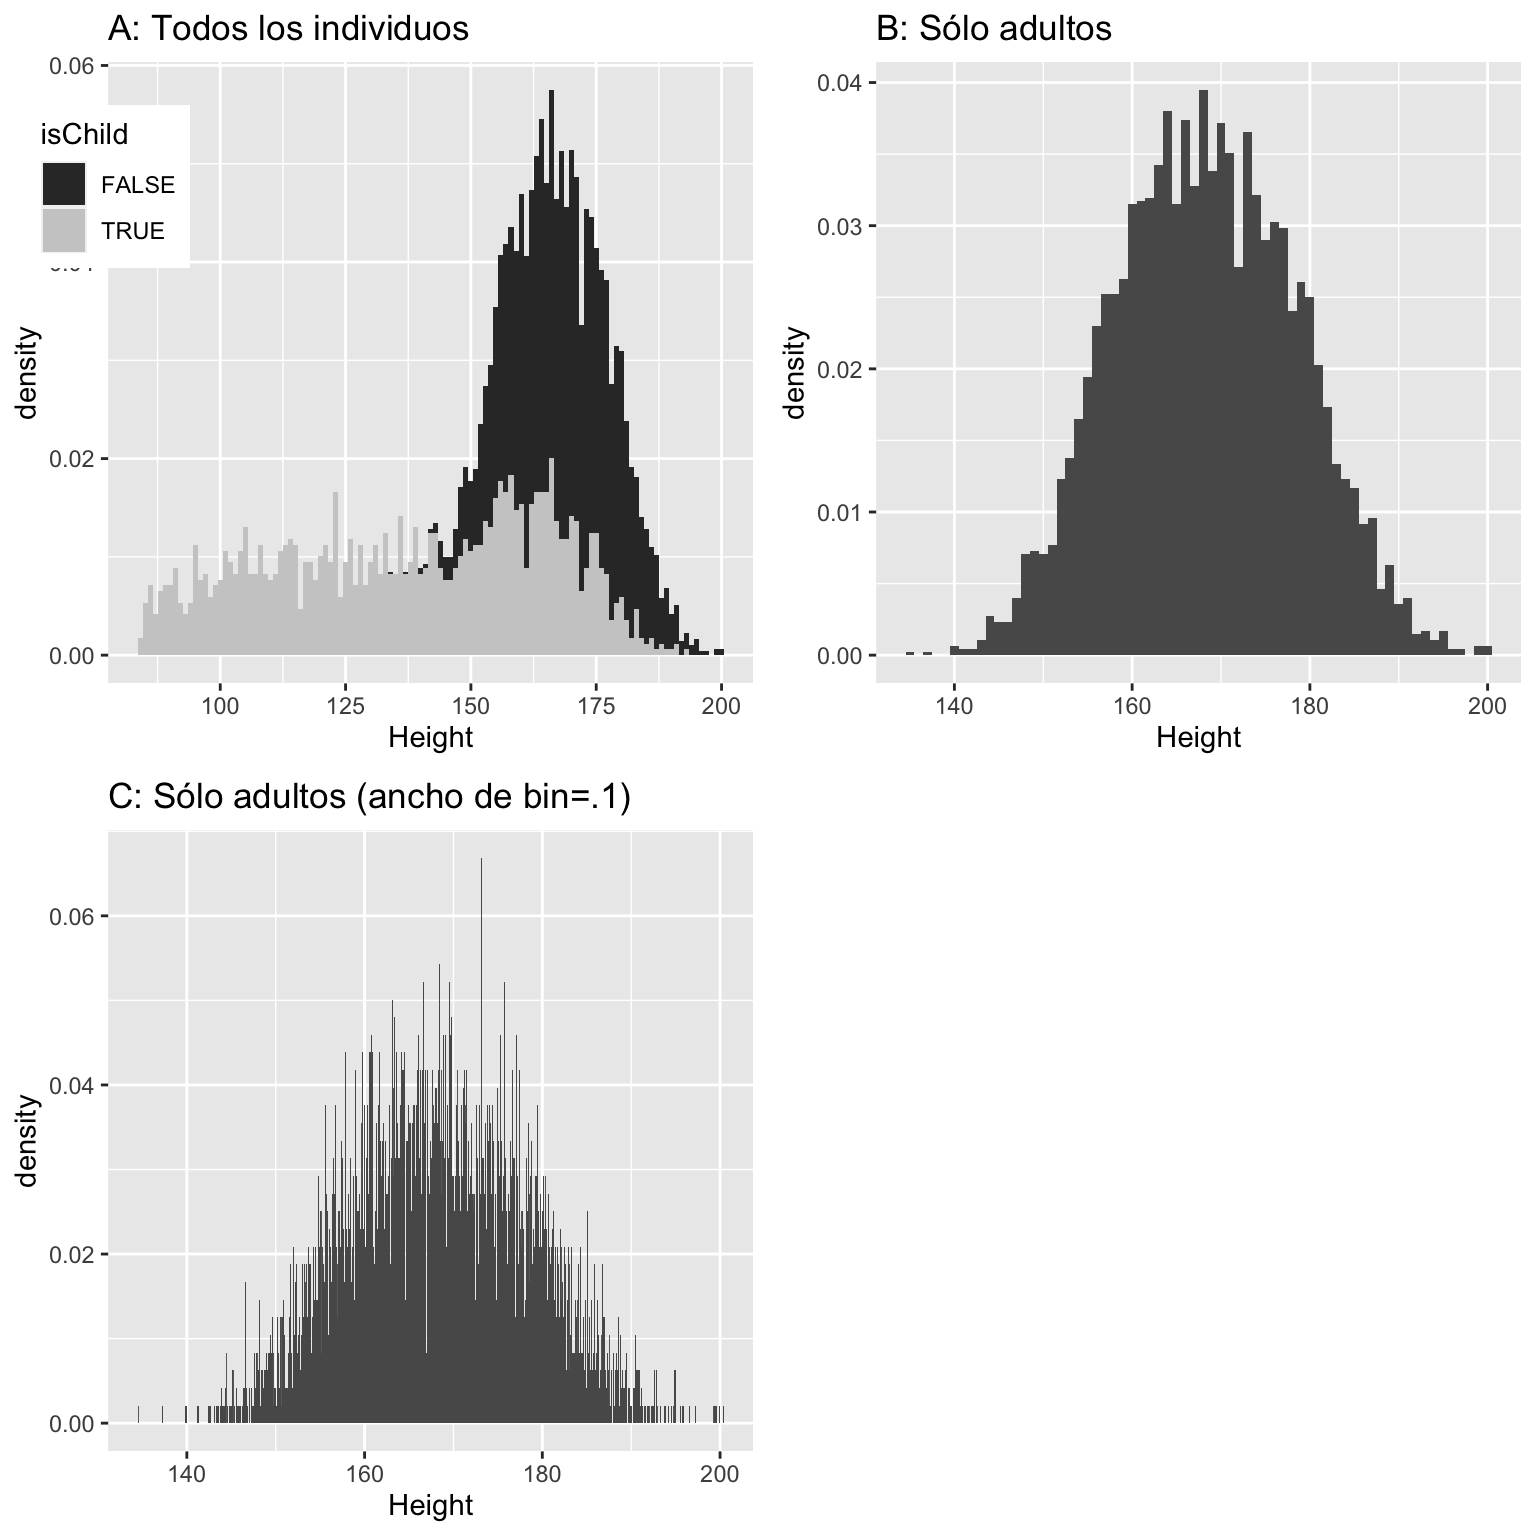
\includegraphics[height=0.5\textheight]{StatsThinking21_files/figure-latex/heightHistSep-1} \caption{Histograma de las alturas en NHANES. A: Valores graficados separando niños y niñas (gris) y adultos (negro). B: Valores sólo para adultos. C: Igual que B, pero con ancho de bins = 0.1}\label{fig:heightHistSep}
\end{figure}

\hypertarget{bins-de-un-histograma}{%
\subsection{Bins de un histograma}\label{bins-de-un-histograma}}

En nuestro ejemplo anterior con la variable de sueño, los datos fueron reportados en números enteros, y nosotros simplemente contamos el número de personas que reportaron cada valor posible. Sin embargo, si observas algunos de los valores en la variable de Altura en NHANES, verás que fueron medidos en centímetros hasta la primera posición decimal:

\begin{table}

\caption{\label{tab:unnamed-chunk-10}Algunos valores de la base de datos NHANES.}
\centering
\begin{tabular}[t]{l}
\hline
Height\\
\hline
169.6\\
\hline
169.8\\
\hline
167.5\\
\hline
155.2\\
\hline
173.8\\
\hline
174.5\\
\hline
\end{tabular}
\end{table}

El panel C de la Figura \ref{fig:heightHistSep} muestra un histograma que cuenta la densidad de cada posible valor. El histograma se ve muy irregular, esto es por la variabilidad en los valores decimales específicos. Por ejemplo, el valor 173.2 ocurre 32 veces, mientras que el valor 173.3 ocurre sólo 15 veces. Probablemente no vamos a pensar que existe una diferencia tan grande entre la prevalencia de estas dos alturas; lo más probable es que esto se deba a variabilidad aleatoria en nuestra muestra de personas.

En general, cuando creamos un histograma de datos que son continuos o donde se tienen muchos valores posibles, crearemos \emph{bins} con los valores para que en lugar de contar y graficar la frecuencia de cada valor específico, contaremos y graficaremos la frecuencia de valores que caen dentro de un rango específico. Esa es la razón por la cual se ve menos irregular la gráfica arriba en el Panel B de la Figura \ref{fig:heightHistSep}; en este panel establecimos el ancho de los bins en 1, lo que significa que el histograma es calculado al combinar valores dentro de los bins con un ancho de uno; por lo que los valores 1.3, 1.5, 1.6 contarían en la frecuencia de un mismo bin, el cual se extendería desde valores iguales a uno hasta valores menores a 2.

Puedes notar que una vez que el tamaño de bin ha sido seleccionado, entonces el número de bins es determinado por los datos:

\[
número\, de\, bins  = \frac{rango\, de\, valores}{ancho\, de\, bin}
\]

No existe una regla rígida u objetiva para escoger el ancho de bins óptimo. Ocasionalmente será obvio (como cuando sólo existen unos pocos valores posibles), pero en muchos casos requerirá ensayo y error. Existen métodos para tratar de encontrar un tamaño de bin óptimo de manera automática, como el método Freedman-Diaconis que usaremos en algunos ejemplos más adelante.

\hypertarget{representaciones-idealizadas-de-distribuciones}{%
\section{Representaciones idealizadas de distribuciones}\label{representaciones-idealizadas-de-distribuciones}}

Las bases de datos son como copos de nieve, en que cada una es diferente, a pesar de ello existen patrones que frecuentemente se observan en diferentes tipos de datos. Esto nos permite usar representaciones idealizadas de los datos para resumirlos aún más. Tomemos las alturas de los adultos graficadas en \ref{fig:heightHistSep}, y grafiquémoslas al lado de una variable muy diferente: ritmo cardíaco (latidos por minuto), también medido en NHANES (véase la Figura \ref{fig:NormalDistPlotsWithDist}).

\begin{figure}
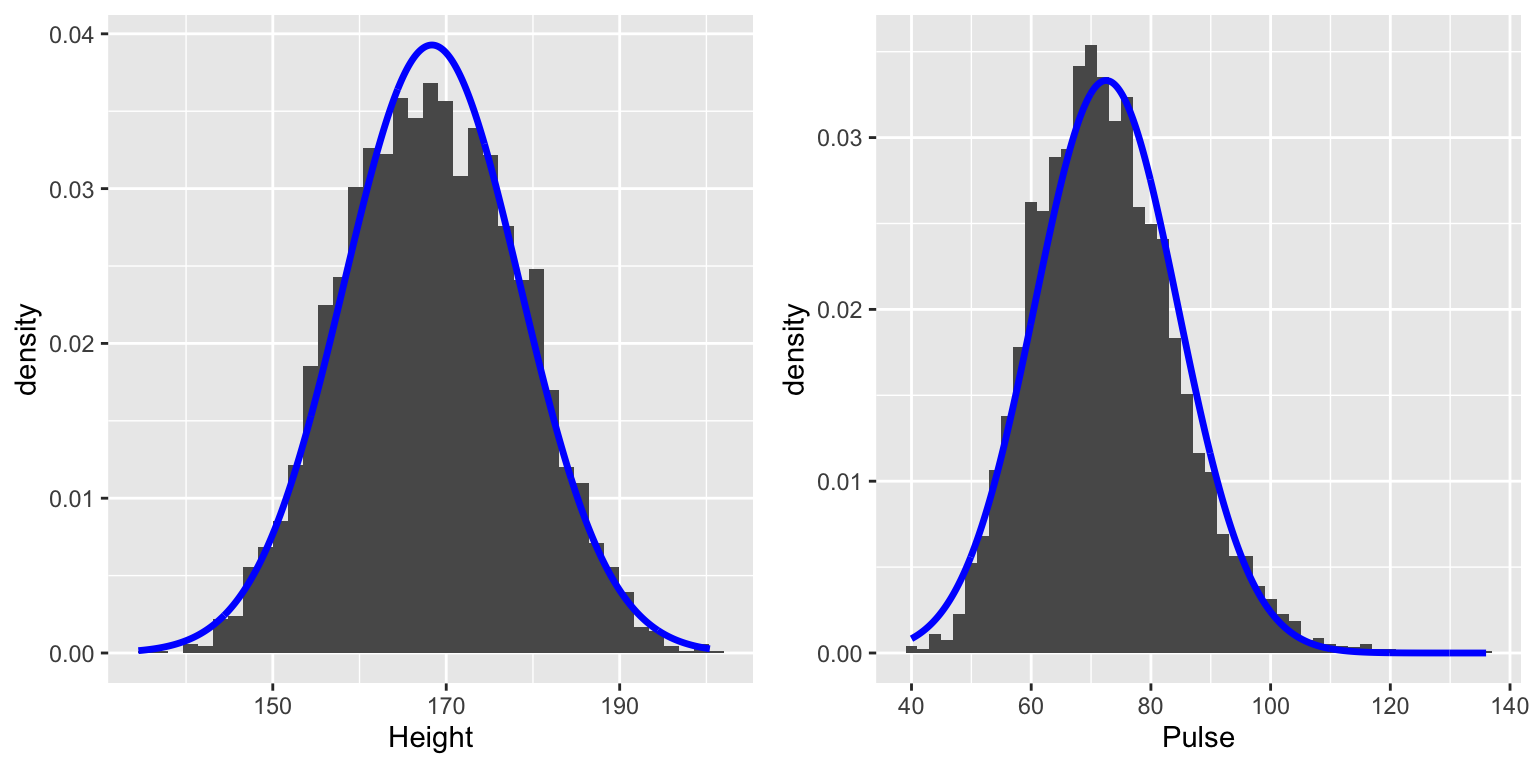
\includegraphics[height=0.5\textheight]{StatsThinking21_files/figure-latex/NormalDistPlotsWithDist-1} \caption{Histogramas de la altura (izquierda) y pulso (derecha) en la base de datos NHANES, con la distribución normal sobrepuesta en cada conjunto de datos.}\label{fig:NormalDistPlotsWithDist}
\end{figure}

Mientras que estas gráficas ciertamente no se ven exactamente iguales, ambas tienen la característica general de ser relativamente simétricas alrededor de un pico redondeado en el medio. De hecho, esta forma es una de las formas de distribuciones comúnmente observadas cuando recolectamos datos, a esta forma se le llama distribución \emph{normal} (o \emph{Gaussiana}). Esta distribución es definida en términos de dos valores (los cuales llamamos \emph{parámetros} de la distribución): la localización del pico central (que llamamos \emph{media}) y el ancho de la distribución (que es descrita en términos de un parámetro llamado \emph{desviación estándar}). La Figura \ref{fig:NormalDistPlotsWithDist} muestra la distribución normal apropiada graficada encima de cada uno de los histogramas. Puedes ver que aunque las curvas no se ajustan exactamente a los datos, hacen un muy buen trabajo de caracterizar la distribución -- ¡con sólo dos números!

Como veremos más tarde cuando discutamos el teorema del límite central, existe una razón matemática profunda por la cual muchas variables en el mundo exhiben la forma de una distribución normal.

\hypertarget{asimetruxeda-sesgo}{%
\subsection{Asimetría (sesgo)}\label{asimetruxeda-sesgo}}

Los ejemplos en la Figura \ref{fig:NormalDistPlotsWithDist} siguen una distribución normal relativamente bien, pero en muchos casos los datos se desviarán de una manera sistemática de la distribución normal. Una manera en la que los datos se pueden desviar es cuando son asimétricos (o sesgados), cuando una cola de la distribución es más densa que la otra. Nos referimos a esto como ``asimetría'' (o sesgo, ``skewness'' en inglés). La asimetría comúnmente sucede cuando la medida está restringida a ser no-negativa, como cuando estamos contando cosas o midiendo lapsos de tiempo (y por lo tanto la variable no puede tomar valores negativos).

Un ejemplo de asimetría se puede ver en el promedio de tiempos de espera en las líneas de seguridad aeropuertaria del Aeropuerto Internacional de San Francisco, graficado en el panel izquierdo de la Figura \ref{fig:SFOWaitTimes}. Puedes observar que mientras la mayoría de los tiempos son menores a 20 minutos, hay un número de casos donde pueden ser mucho mayores, ¡sobre los 60 minutos! Este es un ejemplo de una distribución ``asimétrica a la derecha'', donde la cola derecha es más larga que la izquierda; este tipo de asimetría es común cuando observamos conteos o tiempos medidos, que no pueden ser menores a cero. Es menos común ver distribuciones ``asimétricas a la izquierda'', pero pueden ocurrir, por ejemplo cuando vemos valores de fracciones que no pueden tomar valores mayores a uno.

\begin{figure}
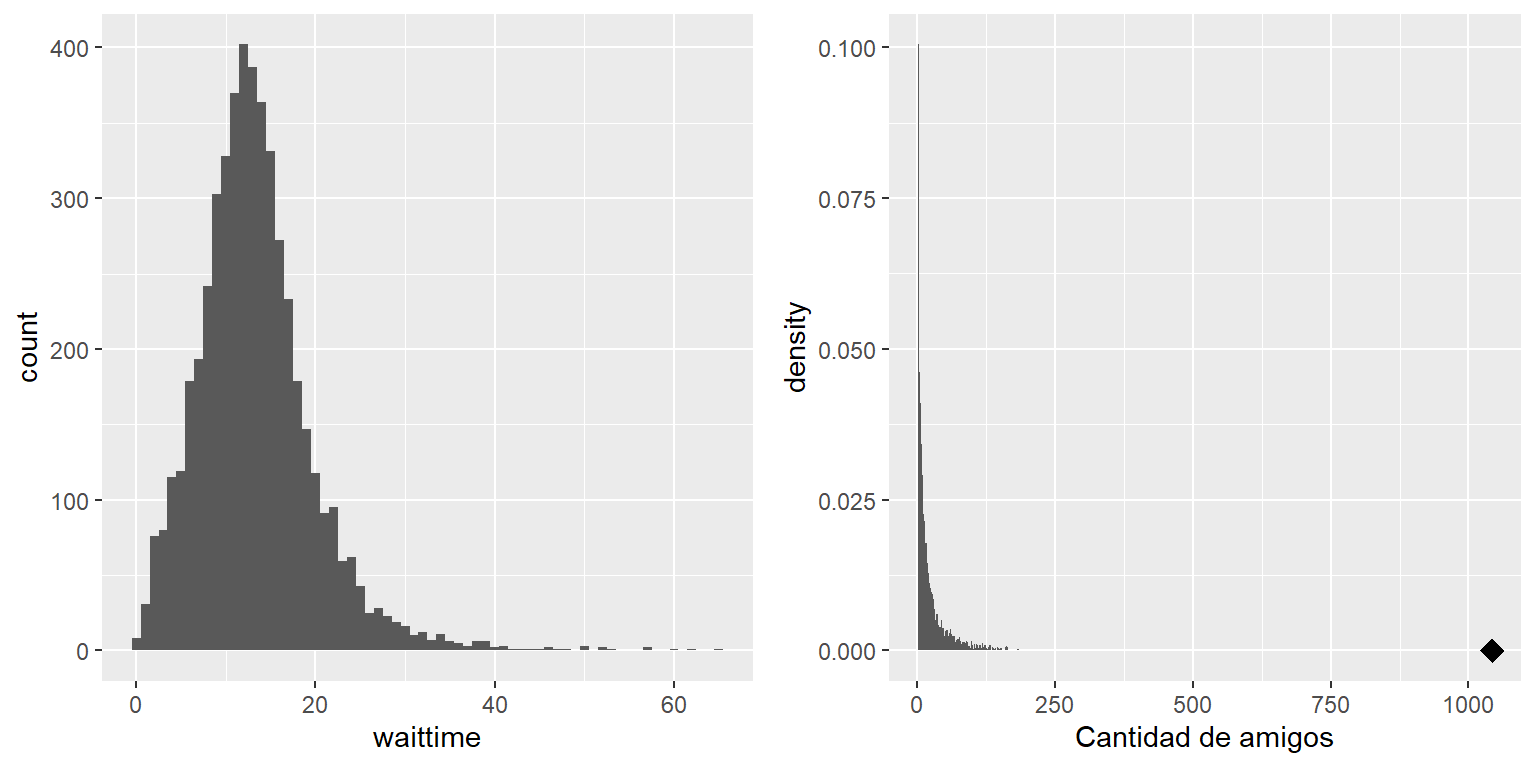
\includegraphics[height=0.5\textheight]{StatsThinking21_files/figure-latex/SFOWaitTimes-1} \caption{Ejemplos de distribuciones asimétricas a la derecha y con cola larga. Izquierda: Tiempo promedio de espera en seguridad en el SFO Terminal A (Enero-Octubre 2017), obtenidos de https://awt.cbp.gov/ . Derecha: Histograma del número de amigos en Facebook entre 3,663 individuos, obtenidos de la Stanford Large Network Database. La persona con el máximo número de amigos está indicada con un diamante.}\label{fig:SFOWaitTimes}
\end{figure}

\hypertarget{distribuciones-con-colas-largas}{%
\subsection{Distribuciones con colas largas}\label{distribuciones-con-colas-largas}}

Históricamente, la estadística se ha enfocado fuertemente en datos que están distribuidos de manera normal, pero existen muchos tipos de datos que no se parecen en nada a la distribución normal. En particular, muchas distribuciones en el mundo real tienen ``cola larga'', esto significa que la cola derecha se extiende mucho más allá de los valores típicos de la distribución. Uno de los tipos de datos más interesantes donde ocurren distribuciones con cola larga suceden del análisis de redes sociales (\emph{social networks}). Para un ejemplo, veamos los datos sobre la cantidad de amigos en Facebook del \href{https://snap.stanford.edu/data/egonets-Facebook.html}{Stanford Large Network Database} y grafiquemos el histograma del número de amigos en una muestra de 3,663 personas en la base de datos (ve el panel derecho de la Figura \ref{fig:SFOWaitTimes}). Como podemos ver, esta distribución tiene una cola derecha muy larga -- la persona promedio tiene 24.09 amigos, ¡mientras que la persona con la mayor cantidad de amigos (marcada por el diamante) tiene 1043!

Distribuciones con cola larga han sido cada vez más reconocidas en el mundo real. En particular, muchas características de sistemas complejos son caracterizadas por estas distribuciones, desde la frecuencia de palabras en un texto, hasta el número de vuelos que llegan y salen de diferentes aeropuertos, como la conectividad de redes neuronales. Existen diferentes maneras en que las distribuciones de cola larga pueden suceder, pero una común sucede en casos del llamado ``Efecto Mateo'' de la Biblia Cristiana:

\begin{quote}
Porque al que tiene, le será dado, y tendrá más; y al que no tiene, aun lo que tiene le será quitado. - Mateo 25:29, Reina Valera 1960.
\end{quote}

Esto frecuentemente es parafraseado como ``los ricos se enriquecen más''. En estas situaciones, las ventajas se combinan o multiplican, de tal manera que aquellos con más amigos tienen acceso aún a más amigos nuevos, y aquellos con más dinero tienen la habilidad de hacer cosas que incrementen sus riquezas aún más.

Conforme el curso avance veremos varios ejemplos de distribuciones de cola larga, y deberemos mantener en mente que muchas de las herramientas en estadística pueden fallar cuando nos enfrentamos con datos con cola larga. Como Nassim Nicholas Taleb señala en su libro ``The Black Swan'', estas distribuciones de cola larga jugaron un papel crítico en la crisis financiera de 2008, porque muchos de los modelos financieros usados por los \emph{traders} (operadores de inversiones) asumieron que los sistemas financieros seguirían una distribución normal, que claramente no siguieron.

\hypertarget{objetivos-de-aprendizaje-2}{%
\section{Objetivos de aprendizaje}\label{objetivos-de-aprendizaje-2}}

Habiendo leído este capítulo, deberías ser capaz de:

\begin{itemize}
\tightlist
\item
  Calcular distribuciones de frecuencia absolutas, relativas, y acumuladas para un conjunto de datos.
\item
  Generar una representación gráfica de una distribución de frecuencias.
\item
  Describir la diferencia entre una distribución normal y una distribución con cola larga, y describir las situaciones que comúnmente dan lugar a cada tipo de distribución.
\end{itemize}

\hypertarget{lecturas-sugeridas-2}{%
\section{Lecturas sugeridas}\label{lecturas-sugeridas-2}}

\begin{itemize}
\tightlist
\item
  \emph{The Black Swan: The Impact of the Highly Improbable}, by Nassim Nicholas Taleb
\end{itemize}

\hypertarget{data-visualization}{%
\chapter{Visualización de Datos}\label{data-visualization}}

El 28 de enero de 1986, el Space Shuttle Challenger explotó 73 segundos después del despegue, matando a lxs 7 astronautas a bordo. Así como cuando los desastres suceden, hubo una investigación oficial sobre lo que ocasionó el accidente. El cual encontró que un ``O-ring'' que conectaba dos secciones del sólido populsor de cohete se fugó, lo cual resultó en la falla de la unión y explosión del tanque propulsor (véase figura \ref{fig:srbLeak}).

\begin{figure}
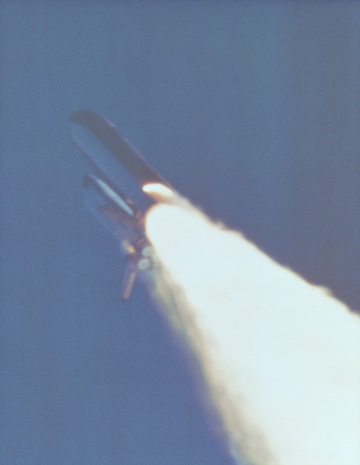
\includegraphics[height=0.2\textheight]{images/Booster_Rocket_Breach_-_GPN-2000-001425} \caption{Imagen del sólido propulsor de cohete fugando combustible, segundos antes de la explosión. By NASA (Great Images in NASA Description) [Public domain], via Wikimedia Commons}\label{fig:srbLeak}
\end{figure}

La investigación encontró que muchos aspectos del proceso de decisión de la NASA tenía errores, y estaban focalizados en una junta entre el personal de la NASA e ingenierxs de Morton Thiokol, un empresario que construía sólidos propulsores de cohete. Estxs ingenierxs estaban paricularmente preocupades por las temperaturas que habían sido pronosticadas para la mañana del lanzamiento, las cuales eran muy bajas. Ellos tenían datos de lanzamientos pasados donde el funcionamiento de los ``O-rings'' se comprometía a temperaturas bajas. En la junta previa al lanzamiento, lxs ingenierxs presentaron sus datos a lxs directivxs de la NASA, pero fueron incapaces de convencerles postponer el lanzamiento. Su evidencia fue una serie de notas escritas a mano mostrando números de los lanzamientos pasados.

El experto en visualización Edward Tufte ha argumentado que con la presentación adecuada de todos los datos, lxs ingenierxs pudieron haber sido mucho más persuasivos. En particular, pudieron haber mostrado una gráfica como la de la Figura \ref{fig:challengerTemps}, en la cual subraya dos hechos importantes. Primero, demuestra la cantidad del daño de ``O-ring'' (definido por la cantidad de erosión y hollín encontrado afuera de los anillos después que el sólido de propulsor de cohete fuera recuperado del océano en vuelos pasados) fue relacionado estrechamente a la temperatura del despegue. Segundo, demuestra que el rango de temperaturas pronosticadas para la mañana del 28 de enero (mostrado en el área sombreada) estaba fuera del rango de todos despegues previos. Mientras que no podemos saber con certeza, parece ser que es posible que hubieran sido más convincentes.

\begin{figure}
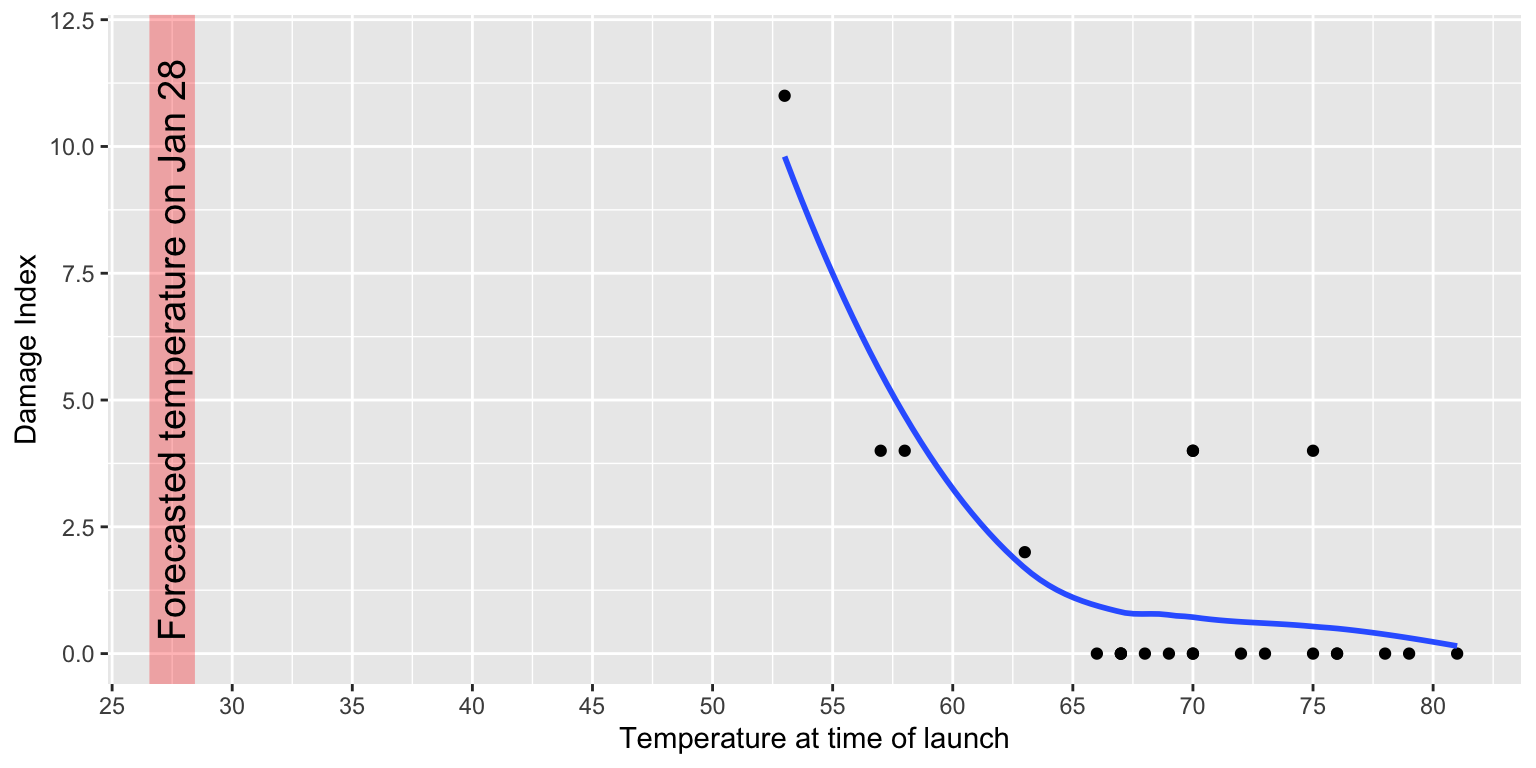
\includegraphics[height=0.5\textheight]{StatsThinking21_files/figure-latex/challengerTemps-1} \caption{Replanteo de los datos del índice de daños de Tufte. La línea muestra la tendencia en los datos y el parche sombreado muestra las temperaturas proyectadas para la mañana del lanzamiento.}\label{fig:challengerTemps}
\end{figure}

\hypertarget{anatomuxeda-de-una-gruxe1fica}{%
\section{Anatomía de una gráfica}\label{anatomuxeda-de-una-gruxe1fica}}

El objetivo de graficar datos es presentar un resumen de una base de datos en una presentación bi-dimensional (o en ocasiones, tri-dimensional). Nos referimos a las dimensiones como \emph{ejes} -- el eje horizontal es llamado el \emph{eje X} y el eje vertical es llamado el \emph{eje Y}. Podemos acomodar los datos a través de los ejes que enfaticen los valores de los datos. Estos valores pueden ser continuos o categóricos.

Hay muchos tipos de gráficas que se pueden utilizar, las cuales tienen diferentes ventajas y desventajas. Digamos que estamos interesades en caracterizar la diferencia de altura en hombres y mujeres en la base de datos NHANES. La figura \ref{fig:plotHeight} muestra cuatro diferentes maneras de graficar esos datos.

\begin{enumerate}
\def\labelenumi{\arabic{enumi}.}
\tightlist
\item
  La gráfica de barras en el panel A muestra la diferencia en medias (means), pero no nos muestra cuánta dispersión hay en los datos alrededor de estas medias -- y como veremos después, saber esto es esencial para determinar si consideramos la diferencia entre el grupo es suficientemente grande como para ser importante.
\end{enumerate}

\begin{enumerate}
\def\labelenumi{\arabic{enumi}.}
\setcounter{enumi}{1}
\tightlist
\item
  La segunda gráfica muestra las barras con todos los puntos de datos (data points) sobrepuestos - esto hace un poco más claro que la distribución por altura entre hombres y mujeres están sobrepuestos, pero aún es difícil ver por la grande cantidad de puntos de datos.\\
  En general preferimos usar una técnica de graficado que provea una vista más clara de la distribución de puntos de datos.
\end{enumerate}

\begin{enumerate}
\def\labelenumi{\arabic{enumi}.}
\setcounter{enumi}{2}
\tightlist
\item
  En el panel C, podemos ver un ejemplo de \emph{gráfica violín}, en la cual se grafica la distribución de cada condición de los datos (después de suavizarla un poco).
\end{enumerate}

\begin{enumerate}
\def\labelenumi{\arabic{enumi}.}
\setcounter{enumi}{3}
\tightlist
\item
  Otra opción es el \emph{diagrama de caja} (box plot) mostrado en el panel D, en el cual muestra la mediana (línea central), una medida de variabilidad (lo ancho de la caja, que esta basado en una medida llamada rango intercuartílico), y cualquier calor atípico (observado por los puntos al final de las líneas). Ambas son formas efectivas de mostrar datos que proporcionan una buena idea de la distribución de los datos.
\end{enumerate}

\begin{figure}
\centering
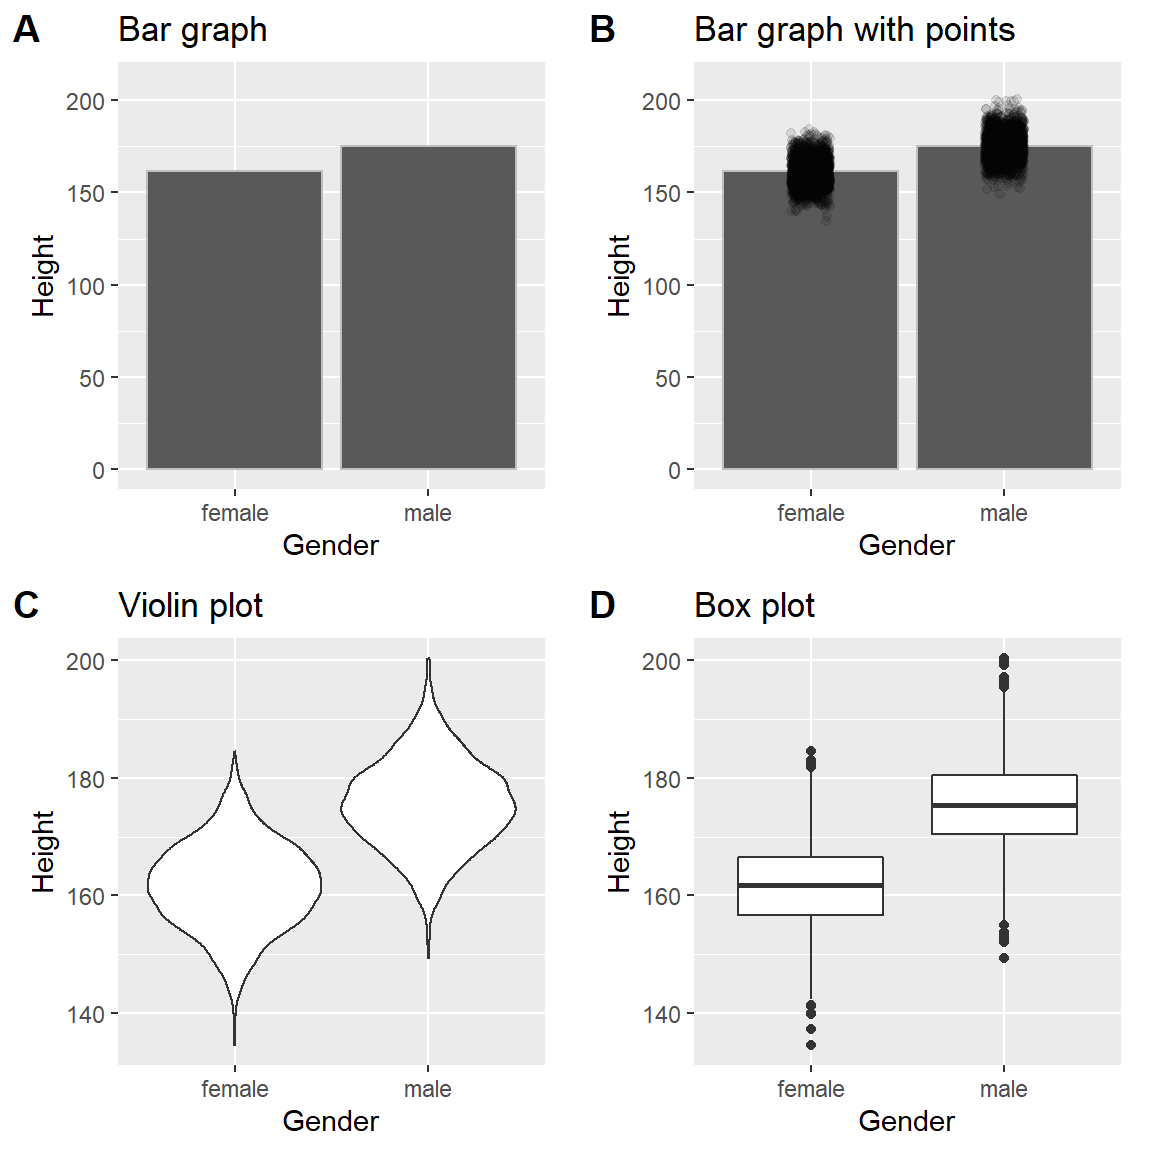
\includegraphics{StatsThinking21_files/figure-latex/plotHeight-1.pdf}
\caption{\label{fig:plotHeight}Four different ways of plotting the difference in height between men and women in the NHANES dataset. Panel A plots the means of the two groups, which gives no way to assess the relative overlap of the two distributions. Panel B shows the same bars, but also overlays the data points, jittering them so that we can see their overall distribution. Panel C shows a violin plot, which shows the distribution of the datasets for each group. Panel D shows a box plot, which highlights the spread of the distribution along with any outliers (which are shown as individual points).}
\end{figure}

\hypertarget{principios-de-una-buena-visibilizaciuxf3n}{%
\section{Principios de una buena visibilización}\label{principios-de-una-buena-visibilizaciuxf3n}}

Se han escrito muchos libros acerca de la visualización efectiva de los datos. Hay algunos principios en los que la mayoría de lxs autorxs están de acuerdo, mientras que otros son más polémicos. Aquí resumimos algunos de los principios fundamentales; si quieres aprender más, entonces algunos buenos recursos están enlistados en la sección de \emph{Lecturas sugeridas} al final del capítulo.

\hypertarget{muestra-los-datos-y-haz-que-destaquen}{%
\subsection{Muestra los datos y haz que destaquen}\label{muestra-los-datos-y-haz-que-destaquen}}

Digamos que llevo a cabo un estudio en donde se examine la relación entre salud dental y el tiempo invertido en el uso de hilo dental, y quiero visualizar los datos. Figura \ref{fig:dentalFigs} muestra cuatro posibles presentaciones de estos datos.

\begin{enumerate}
\def\labelenumi{\arabic{enumi}.}
\tightlist
\item
  En el panel A, en realidad no mostramos los datos, sólo una línea expresando la relación entre los datos. Esto claramente no es óptimo, porque en realidad no podemos ver cómo se ven los datos subyacentes.
  Los paneles B-D muestran tres posibles resultados de graficar los datos, en donde cada gráfica muestra una manera diferente en la que los datos se pudieron haber visto.
\end{enumerate}

\begin{enumerate}
\def\labelenumi{\arabic{enumi}.}
\setcounter{enumi}{1}
\item
  Si vemos la gráfica en el panel B, puede que desconfiemos -- pocas veces datos reales siguen un patrón preciso.
\item
  Los datos en el panel C, por el otro lado, se ven como datos reales -- muestran una tendencia general, pero son desordenados, como suelen ser los datos en el mundo real.
\item
  Los datos en el panel D nos muestran, aparentemente que la relación entre las dos variables es solamente causada por un inviduo, al que nos referiremos como \emph{atípico} (outlier) porque cae muy lejos del patrón del resto del grupo. Debería de ser claro que probablemente no queremos sacar muchas conclusiones de un efecto guiado por un solo punto de los datos. Esta figura resalta por qué es \emph{siempre} importante mirar los datos sin procesar antes de confiar demasiado en cualquier resumen de los datos.
\end{enumerate}

\begin{figure}
\centering
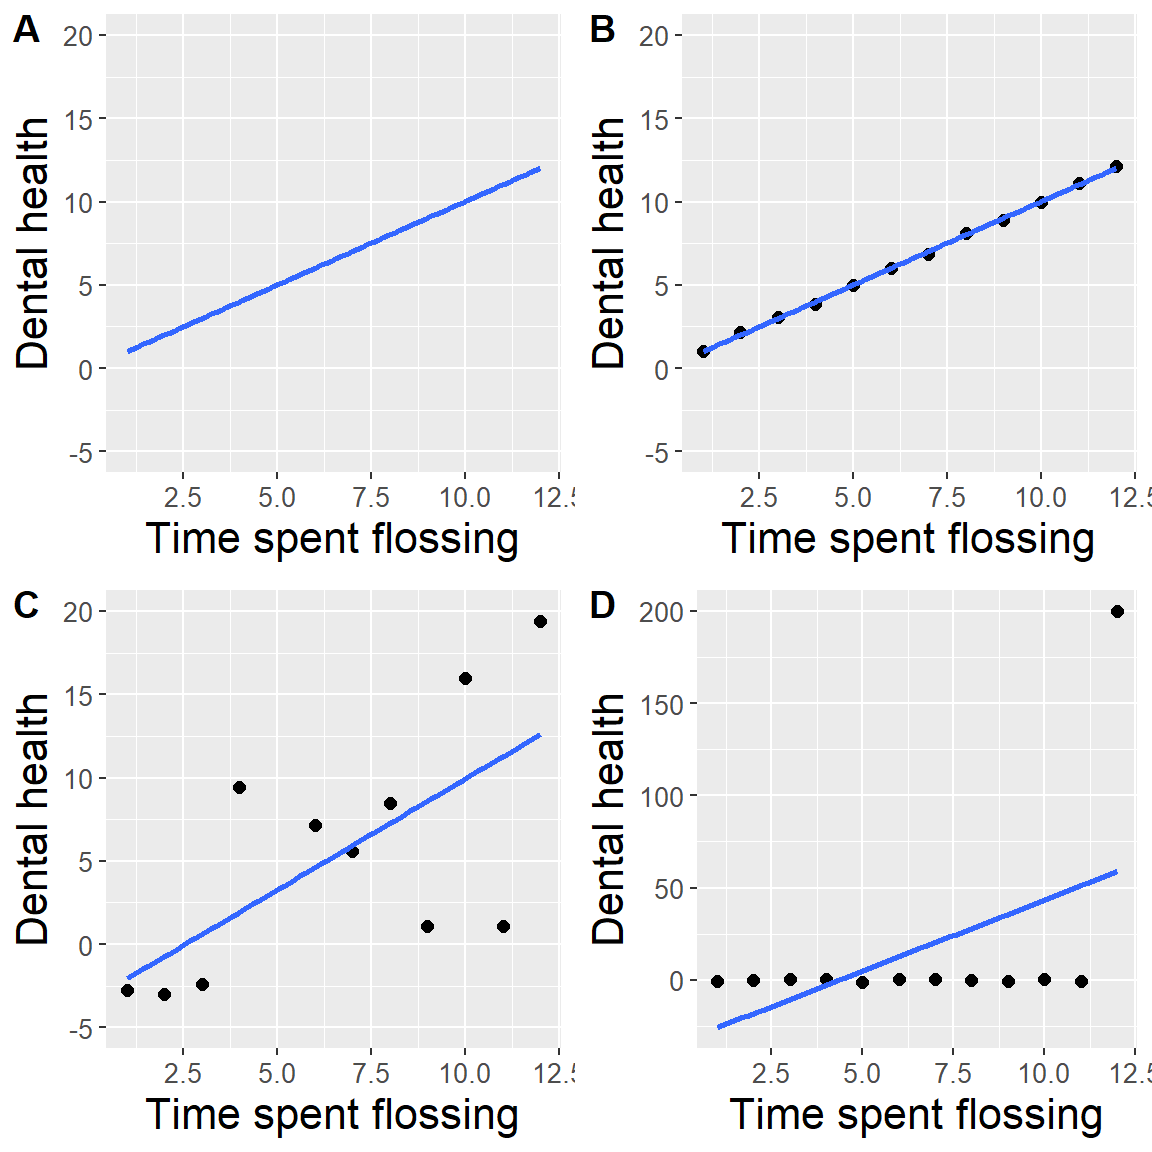
\includegraphics{StatsThinking21_files/figure-latex/dentalFigs-1.pdf}
\caption{\label{fig:dentalFigs}Cuatro posibles presentaciones diferentes de datos para el ejemplo de salud dental. Cada punto del gráfico de dispersión representa un punto de datos en el conjunto de datos y la línea en cada gráfico representa la tendencia lineal en los datos.}
\end{figure}

\hypertarget{maximizar-la-porporciuxf3n-datostinta-dataink-ratio}{%
\subsection{Maximizar la porporción datos/tinta (data/ink ratio)}\label{maximizar-la-porporciuxf3n-datostinta-dataink-ratio}}

Edward Tufte propuso la idea llamada \emph{proporción datos/tinta} (\emph{data/ink ratio})
\[
data/ink\ ratio = \frac{amount\, of\, ink\, used\, on\, data}{total\, amount\, of\, ink}
\]
El punto de esto es minimizar la contaminazión visual y dejar mostrar los datos. Por ejemplo, toma las dos presentaciones sobre la salud dental en la Figura \ref{fig:dataInkExample}. Ambos paneles muestran los mismos datos, pero el panel A es mucho más sencillo de comprender, porque es relativamente alta la proporción de datos/tinta.

\begin{figure}
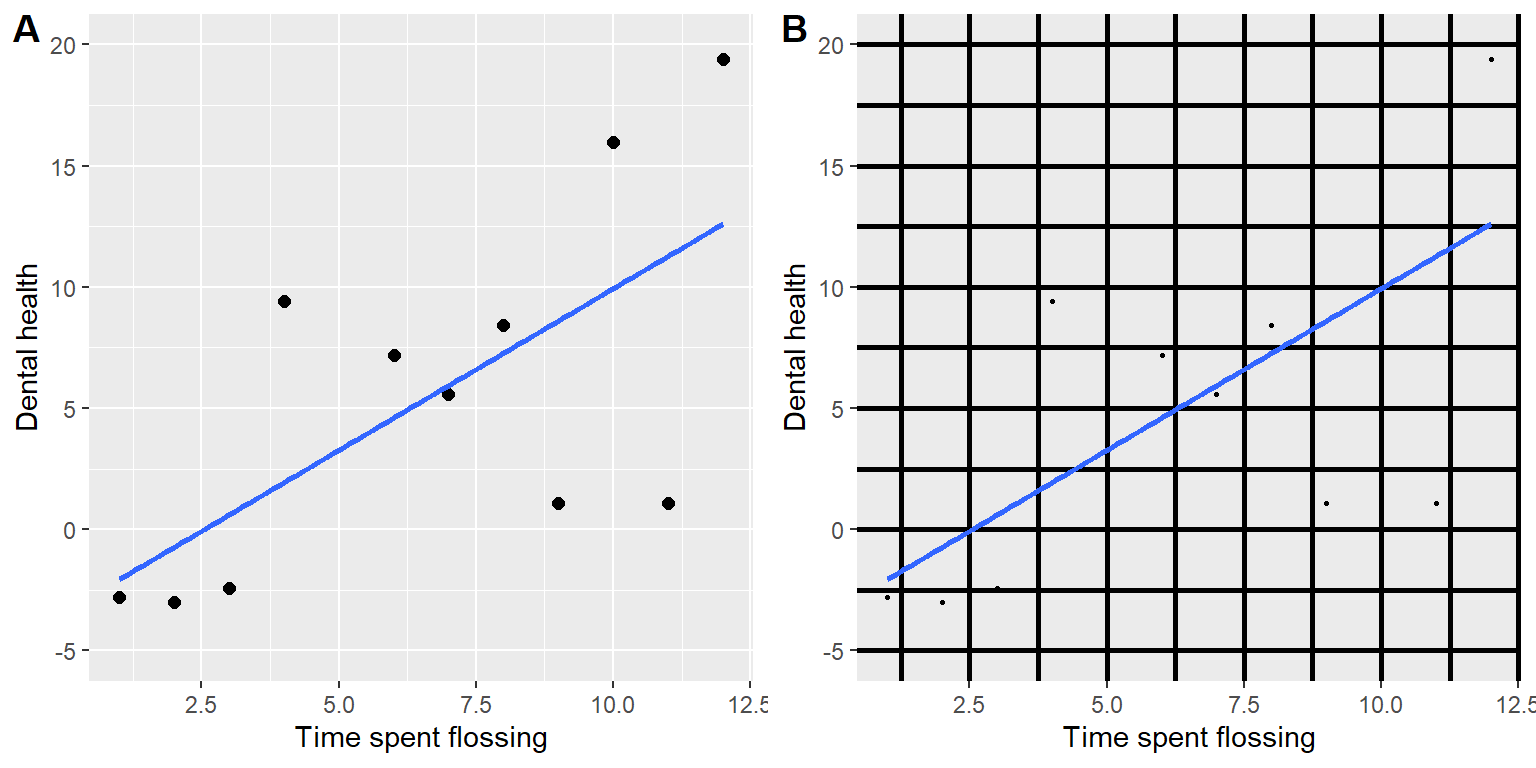
\includegraphics[height=0.5\textheight]{StatsThinking21_files/figure-latex/dataInkExample-1} \caption{Un ejemplo de los mismos datos graficados en dos porporciones datos/tinta diferentes.}\label{fig:dataInkExample}
\end{figure}

\hypertarget{evita-gruxe1ficas-basura}{%
\subsection{Evita gráficas basura}\label{evita-gruxe1ficas-basura}}

Es especialmente común ver presentaciones de datos en medios populares que son adornados con muchos elementos visuales y que son temáticamente relacionados con el contenido pero no relacionados con los datos verdaderos. Esto es conocido como \emph{gráficas basura} (chartjunk) y debe de ser evitado a toda costa.
Una buena manera de no usar gráficas basura es tratar de evitar programas populares de hojas de cálculo para graficar nuestros datos. Por ejemplo el diagrama en la Figura \ref{fig:chartJunk} (creado en Microsoft Excel) grafica la popularidad relativa de las diferentes regiones de Estados Unidos.
Hay al menos tres cosas mal con esta figura:

\begin{itemize}
\tightlist
\item
  tiene gráficos superpuestos en cada una de las barras que no tienen nada que ver con los datos reales
\item
  tiene una textura de fondo que distrae
\item
  utiliza barras tridimensionales, que distorsionan los datos
\end{itemize}

\begin{figure}
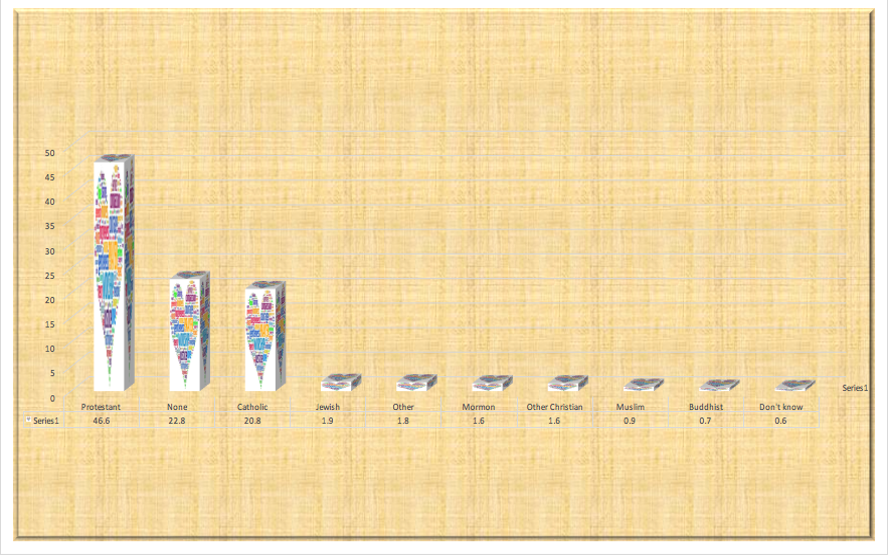
\includegraphics[width=0.8\linewidth,height=0.5\textheight]{images/excel_chartjunk} \caption{An example of chart junk.}\label{fig:chartJunk}
\end{figure}

\hypertarget{evita-distorsionar-los-datos}{%
\subsection{Evita distorsionar los datos}\label{evita-distorsionar-los-datos}}

En ocasiones es posible usar la visualización para distorsionar el mensaje de un conjunto de datos. Algo muy común es el uso de diferentes escalas de eje para exagerar u ocultar un patrón de datos. Por ejemplo, digamos que estamos interesades en ver si los índices de crímenes violentos han cambiado en Estados Unidos. En la Figura \ref{fig:crimePlotAxes}, podemos ver los datos graficados de manera que parece ser que el crimen ha permanecido constante, o que se ha desplomado.¡Los mismos datos pueden contar dos historias muy diferentes!

\begin{figure}
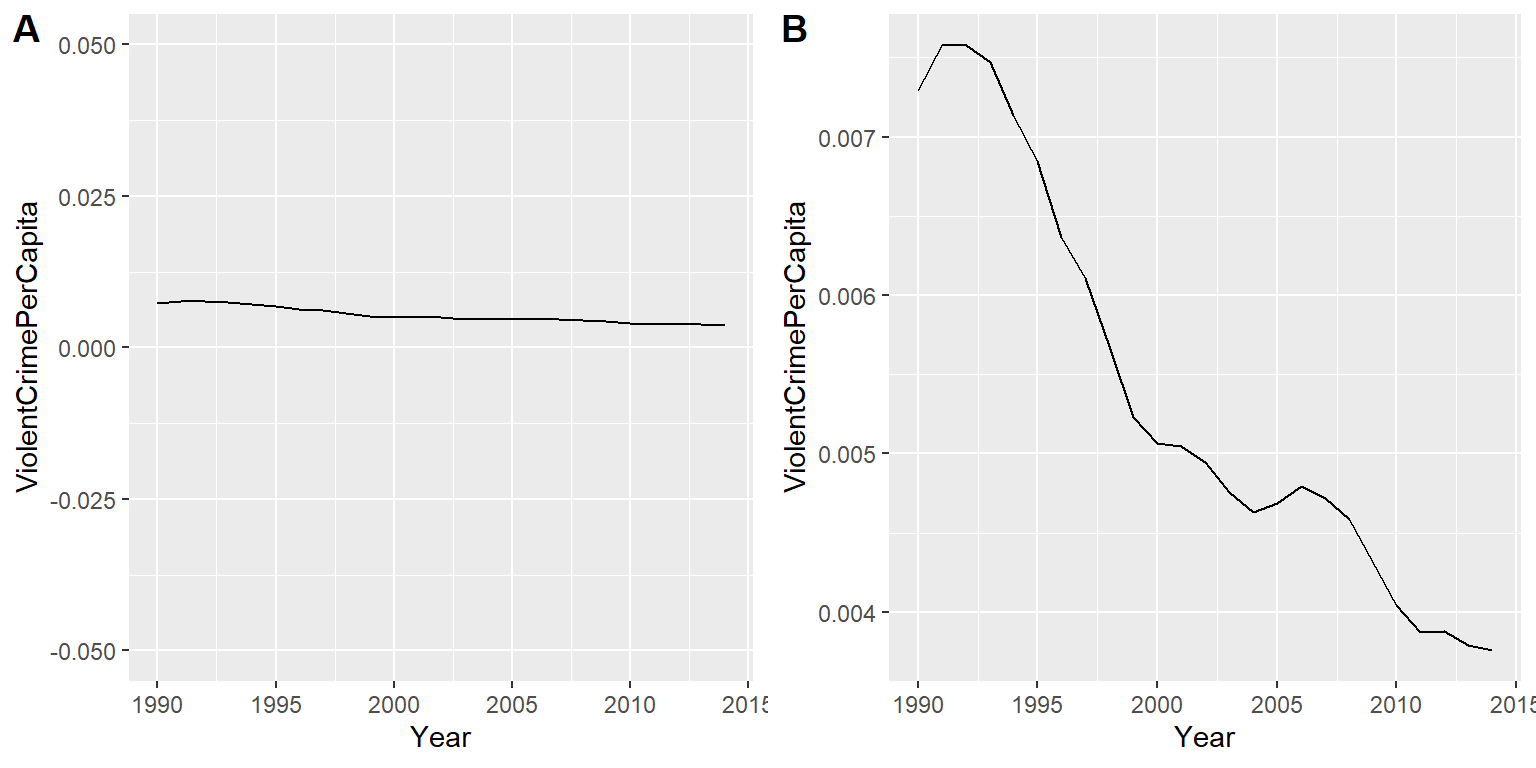
\includegraphics[height=0.5\textheight]{StatsThinking21_files/figure-latex/crimePlotAxes-1} \caption{Datos de crimen de 1990 a 2014 graficados con el tiempo. Los paneles A y B muestran los mismos datos pero con diferentes rangos de eje. Datos obtenidos de https://www.ucrdatatool.gov/Search/Crime/State/RunCrimeStatebyState.cfm}\label{fig:crimePlotAxes}
\end{figure}

Una de las mayores controversias en la visualización de datos estadísticos es como elegir el eje Y, y en particular si se debe de incluir el cero. En su famoso libro ``Cómo mentir con estadística'', Darrell Huff argumentó fuertemente que uno siempre debería de incluir el cero en el eje Y. Por otro lado, Edward Tufte ha argumentado en contra de esto:

\begin{quote}
``En general, en una serie de tiempo, usa una línea de base que muestre los datos y no el punto cero; no gastes mucho espacio vertical vacío tratando de llegar al punto cero a costa de ocultar lo que está sucediendo en la línea de datos en sí'' (de: \url{https://qz.com/418083/its-ok-not-to-start-your-y-axis-at-zero/}).
\end{quote}

Ciertamente, hay ciertos casos en donde usar el punto cero no tiene sentido para nada. Digamos que estamos interesades en graficar la temperatura corporal de un individuo en el tiempo. En la Figura \ref{fig:bodyTempAxis} graficamos los mismos datos (simulados) con o sin cero en el eje Y. Debería de ser obvio que al graficar estos datos con cero en el eje Y (Panel A) estamos gastando mucho espacio en la figura, ¡dado que la temperatura corporal de una persona viva nunca podría llegar a cero! Al incluir el cero, tambien estamos haciendo el salto de temperatura durante 21-30 días menos evidente. En general, mi inclinación por gráficas lineales y de dispersión es para usar todo el espacio en la gráfica, a menos que el punto cero sea sumamente importante de recalcar.

\begin{figure}
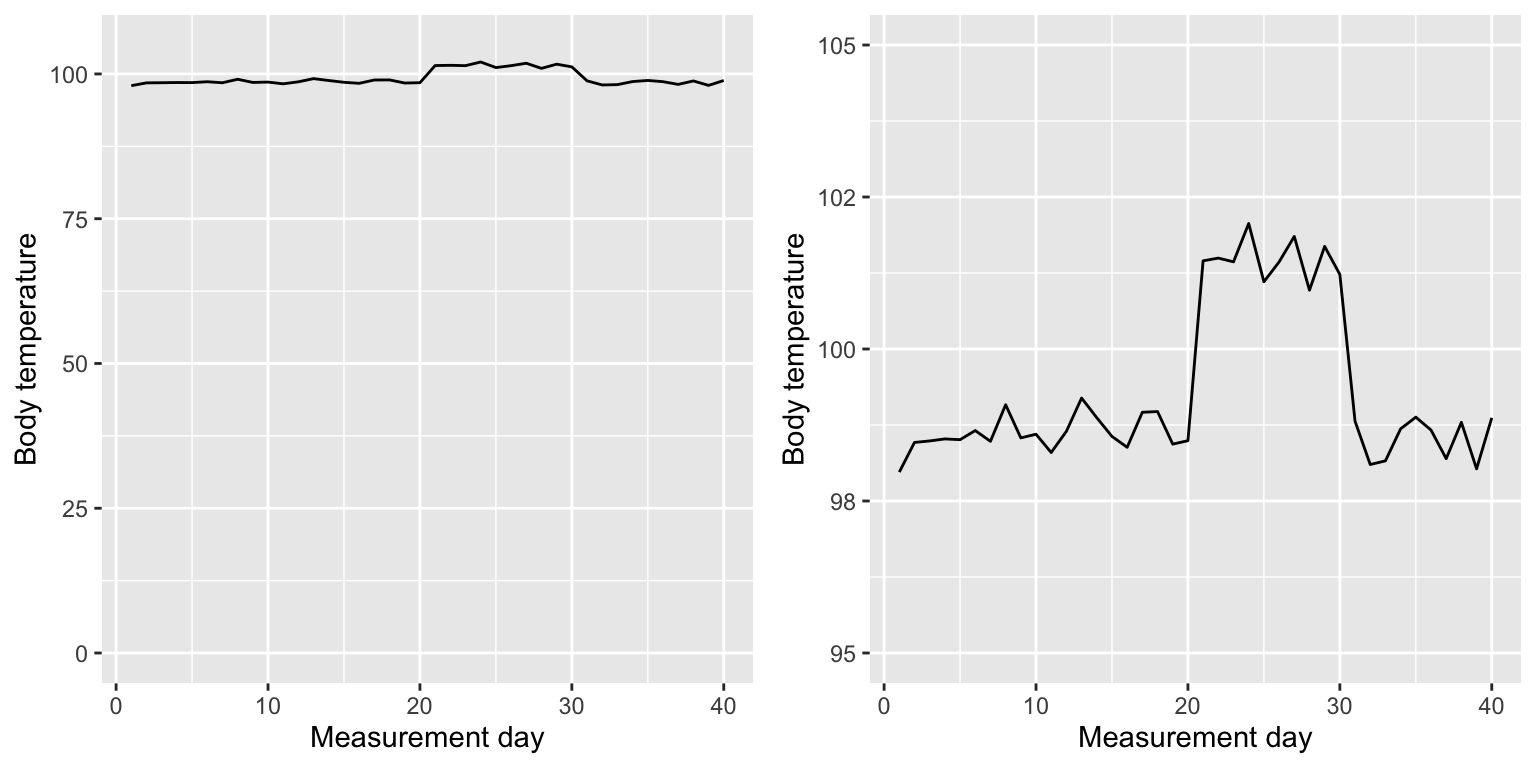
\includegraphics[height=0.5\textheight]{StatsThinking21_files/figure-latex/bodyTempAxis-1} \caption{Temperatura corporal a lo largo del tiempo, graficado con o sin el punto cero en el eje Y.}\label{fig:bodyTempAxis}
\end{figure}

Edward Tufte introdujo el concepto del \emph{factor de engaño} (lie factor) para describir el grado en el cual las diferencias físicas en la visualización corresponden a la magnitud de las diferencias en los datos. Si una gráfica tiene un factor de engaño cercano a 1, entonces es una representación apropiada de los datos, pero si el factor de engaño es lejano a uno refleja una distorsión de los datos subyacentes.

El factor de engaño apoya el argumento de que uno siempre debería de incluir el punto cero en gráfico de barras en muchos casos. En la Figura \ref{fig:barCharLieFactor} graficamos los mismos datos con y sin el cero en el eje Y. En el panel A, la diferencia proporcional del área de las dos barras es exactamente igual a la diferencia proporcional entre los valores (ejemplo, factor de engaño= 1) mientras que en el Panel B (donde el cero no está incluído) la diferencia proporcional en área entre las dos barras es aproximadamente 2.8 veces mayor que la diferencia proporcional de los valores, por lo tanto exagera visualmente el tamaño de la diferencia.

\begin{figure}
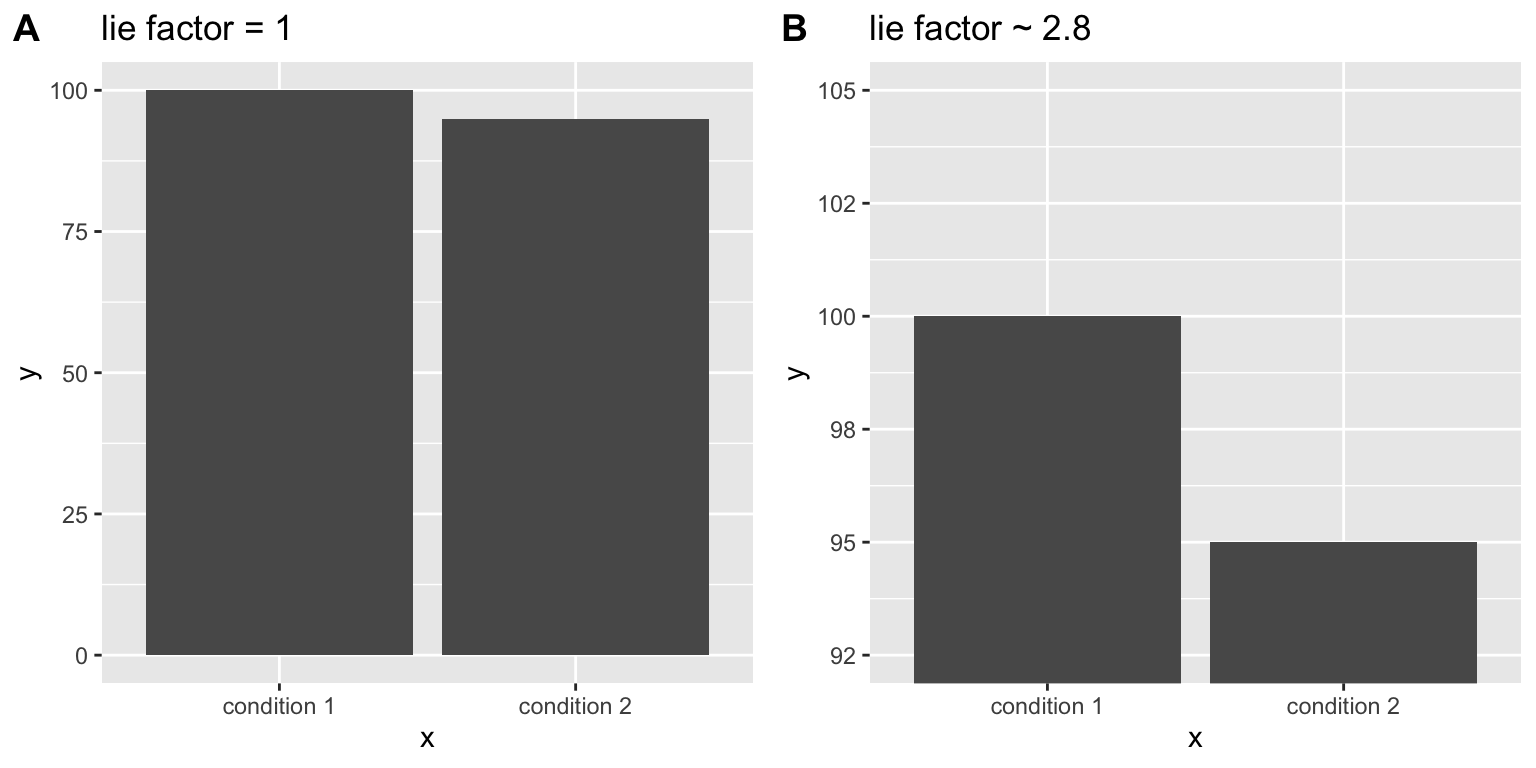
\includegraphics[height=0.5\textheight]{StatsThinking21_files/figure-latex/barCharLieFactor-1} \caption{Dos gráficos de barra con la asociación del factor de engaño }\label{fig:barCharLieFactor}
\end{figure}

\hypertarget{acomodando-las-limitaciones-humanas}{%
\section{Acomodando las limitaciones humanas}\label{acomodando-las-limitaciones-humanas}}

Les humanes tienen limitaciones perceptuales y cognitivas que pueden hacer ciertas visializaciones difíciles de entender. Siempre es importante mantener esto en cuenta cuando se construye la visualización.

\hypertarget{limitaciones-perceptuales}{%
\subsection{Limitaciones perceptuales}\label{limitaciones-perceptuales}}

Una limitación perceptual importante que muchas personas (incluidas yo) sufren es daltonismo. Esto puede hacer muy difícil la percepción de la información en una figura (como la de la Figura \ref{fig:badColors}) donde hay únicamente contraste de color entre los elementos pero no contraste de brillo. Siempre es útil utilizar elementos gráficos que difieran substancialmente en brillo y/o textura en complemento al color. Existen también \href{http://www.cookbook-r.com/Graphs/Colors_(ggplot2)/\#a-colorblind-friendly-palette}{paletas de color amigables con daltónicxs} disponibles para el uso en R.

\begin{figure}
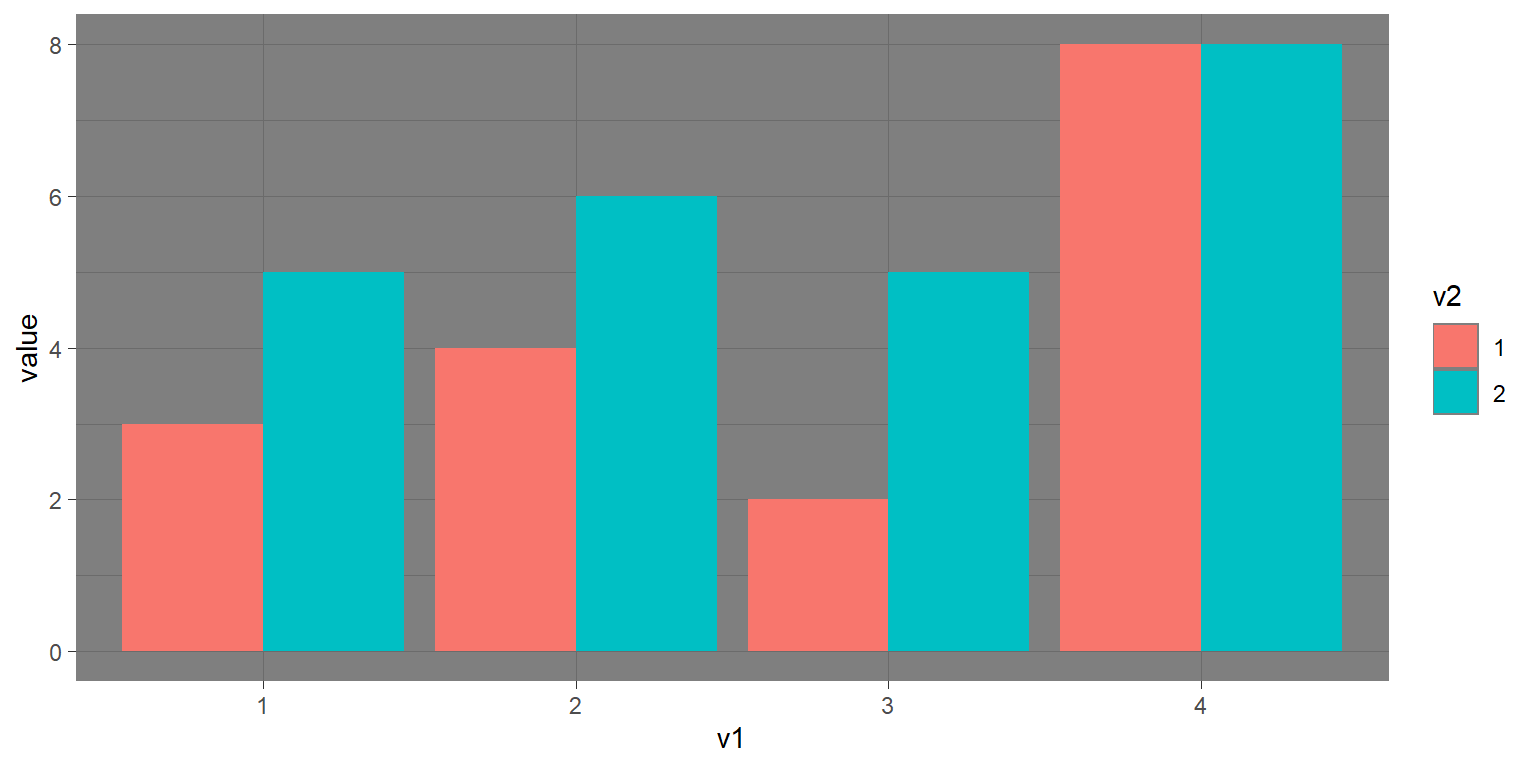
\includegraphics[height=0.5\textheight]{StatsThinking21_files/figure-latex/badColors-1} \caption{Ejemplo de una mala figura que depende únicamente en el contraste de color.}\label{fig:badColors}
\end{figure}

Incluso para personas con visión perfecta, hay algunas limitantes perceptuales que pueden hacer algunas gráficas ineficaces. Esta es una razón por la cual les estadístiques \emph{nunca} usan gráficas circulares o de pastel: Puede ser muy difícil para humanos percibir correctamente las diferencias en el volumen de las formas. La gráfica de pastel en la Figura \ref{fig:pieChart} (presentando los mismos datos en afiliaciones religiosas que mostramos anteriormente) nos muestra que tan complicado puede ser esto.

\begin{figure}
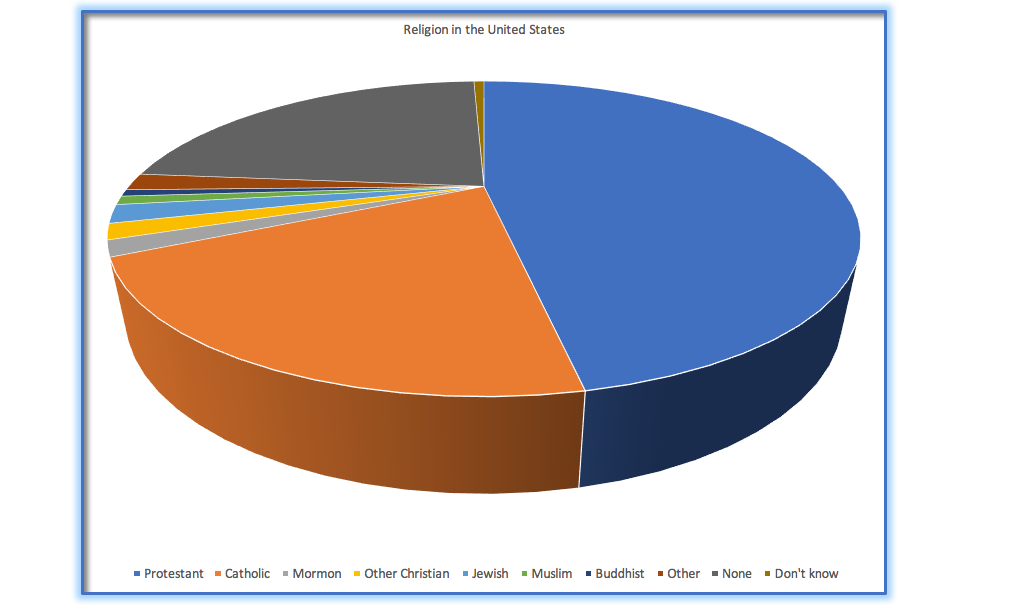
\includegraphics[height=0.5\textheight]{images/religion_piechart} \caption{Un ejemplo de una gráfica de pie, enfatizando la dificultad en comprendiendo el volumen relaticvo de las diferentes rebanadas de pie.}\label{fig:pieChart}
\end{figure}

Esta gráfica es terrible por varias razones. Primero, requiere distinguir un gran número de colores de parches muy pequeños en la parte inferior de la figura. Segundo, la perspectiva visual distorsiona los números relativos, tal como la rebanada de pastel para Católica la cual aparece mucho más grande que la rebanada para Ninguna, cuando en realidad el número para Ninguna es ligeramente mayor (22.8 vs 20.8), como es evidente en la Figura \ref{fig:chartJunk}. Tercero, al separar la leyenda del gráfico, requiere que les lectores retengan información en su memoria de trabajo para poder mapear entre el gráfico y la leyenda y realizar muchas ``búsquedas de tablas'' para hacer coincidir continuamente las etiquetas de la leyenda con la visualización. Y, por último, utiliza texto que es demasiado pequeño, lo que hace que sea imposible leerlo sin hacer zoom.

Graficando los datos usando un enfoque más razonable (Figura \ref{fig:religionBars}), podemos ver el patrón mucho más claramente. Es posible que este gráfico no parezca tan llamativo como el gráfico circular generado con Excel, pero es una representación mucho más eficaz y precisa de los datos.

\begin{figure}
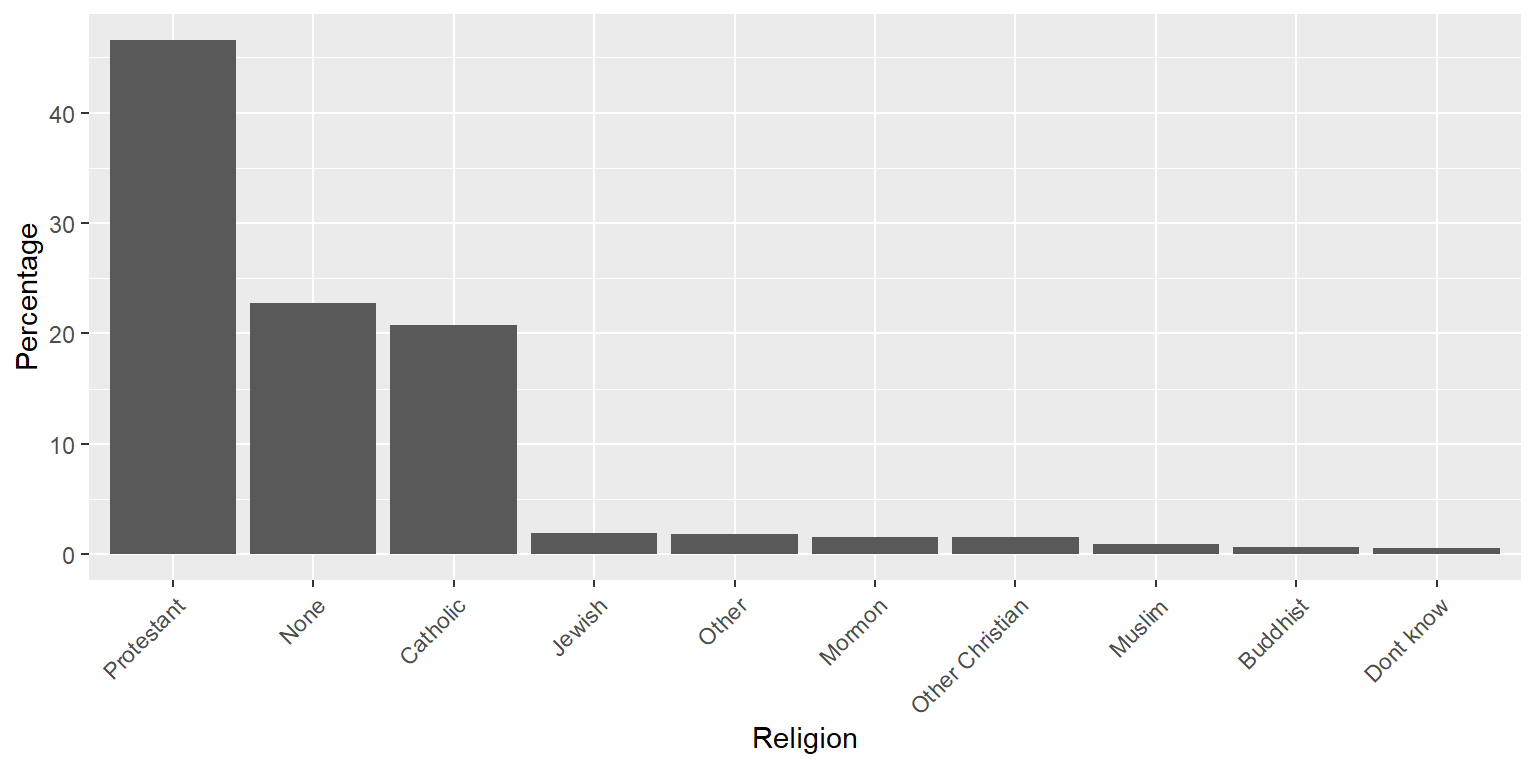
\includegraphics[height=0.5\textheight]{StatsThinking21_files/figure-latex/religionBars-1} \caption{Una presentación más clara de los datos de afiliación religiosa (obtenido de http://www.pewforum.org/religious-landscape-study/).}\label{fig:religionBars}
\end{figure}

Esta gráfica permite al espectador hacer comparaciones basadas en la longitud de las barras a lo largo de una escala común (el eje y). Los seres humanos tienden a ser más precisos al decodificar las diferencias en función de estos elementos perceptivos que en función del área o el color.

\hypertarget{corrigiendo-otros-factores}{%
\section{Corrigiendo otros factores}\label{corrigiendo-otros-factores}}

Comúnmente estamos interesades en graficar datos donde la variable de interés es afectada por otros factores aparte del que nos interesa. Por ejemplo digamos que queremos entender cómo el precio de la gasolina ha cambiado con el paso del tiempo. La figura \ref{fig:gasPrices} muestra datos históricos sobre el precio de la gasolina, graficado con o sin el ajuste de la inflación. Mientras que los datos inajustados muestran un gran incremento, los datos ajustados muestran que es simplemente un reflejo de la inflación. Otros ejemplos donde une necesita ajustar los datos por otros factores incluye el tamaño de la población y datos obtenidos a través de diferentes temporadas.

\begin{figure}
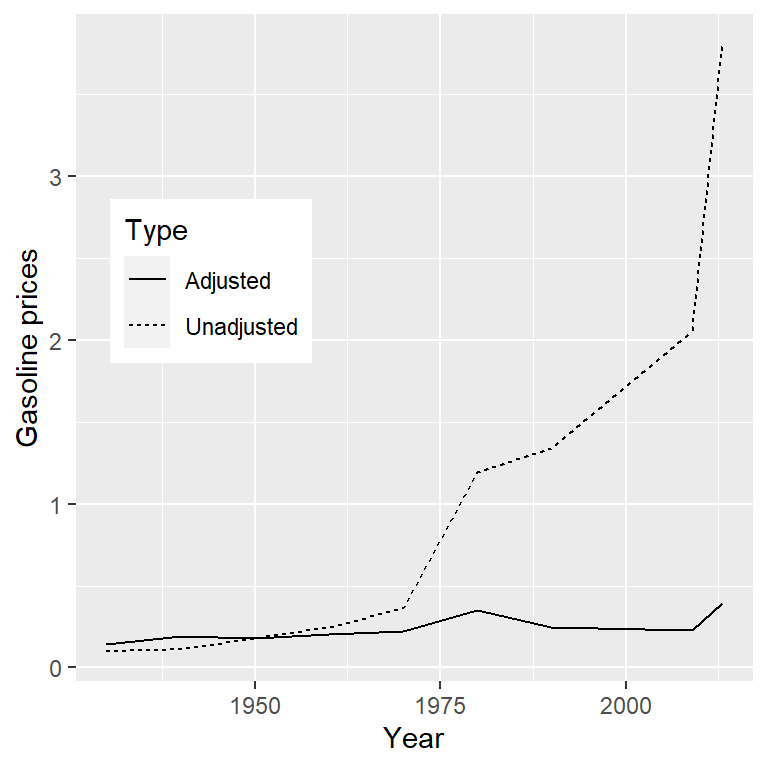
\includegraphics[height=0.5\textheight]{StatsThinking21_files/figure-latex/gasPrices-1} \caption{El precio de la gasolina en Estados Unidos de 1930 a 2013 (obtained from http://www.thepeoplehistory.com/70yearsofpricechange.html) con o sin la corrección para inflación (based on Consumer Price Index).}\label{fig:gasPrices}
\end{figure}

\hypertarget{objetivos-de-aprendizaje-3}{%
\section{Objetivos de aprendizaje}\label{objetivos-de-aprendizaje-3}}

Al leer este capítulo deberás de ser capaz de:

\begin{itemize}
\tightlist
\item
  Describir los principios que distinguen a las buenas y malas gráficas, y usarlos para identificar buenos y malos gráficos.
\item
  Entender las limitaciones humanas que deben de ser acomodadas para hacer gráficas eficaces.
\item
  Prometer nunca crear una gráfica de pastel. \emph{Jamás}.
\end{itemize}

\hypertarget{lecturas-y-videos-sugeridos}{%
\section{Lecturas y videos sugeridos}\label{lecturas-y-videos-sugeridos}}

\begin{itemize}
\tightlist
\item
  \href{https://serialmentor.com/dataviz/}{\emph{Fundamentals of Data Visualization}}, by Claus Wilke
\item
  \emph{Visual Explanations}, by Edward Tufte
\item
  \emph{Visualizing Data}, by William S. Cleveland
\item
  \emph{Graph Design for the Eye and Mind}, by Stephen M. Kosslyn
\item
  \href{https://www.youtube.com/watch?v=fSgEeI2Xpdc\&feature=youtu.be}{\emph{How Humans See Data}}, by John Rauser
\end{itemize}

\hypertarget{fitting-models}{%
\chapter{Ajustar modelos a datos}\label{fitting-models}}

Una de las actividades fundamentales en estadística es crear modelos que puedan resumir datos utilizando un grupo pequeño de números, de esta forma, se provee una descripción compacta de los datos. En este capítulo discutiremos el concepto de lo que es un modelo estadístico y cómo puede ser utilizado para describir datos.

\hypertarget{quuxe9-es-un-modelo}{%
\section{¿Qué es un modelo?}\label{quuxe9-es-un-modelo}}

En el mundo físico, los ``modelos'' son generalmente simplificaciones de cosas del mundo real que, no obstante, transmiten la esencia de lo que se está modelando. El modelo de un edificio transmite la escencia de la estructura del edificio mientras es lo suficientemente pequeño y ligero como para que unx lo pueda sostener con las manos; un modelo de una célula de biología es mucho más grande que una célula real, no obstante, transmite la mayoría de las partes de la célula y las relaciones que tienen entre sí.

En estadística, un modelo tiene el propósito de proveer una descripción similar condensada, pero para los datos, en lugar de una estructura física. Como los modelos físicos, un modelo estadístico es generalmente mucho más simple que los datos que están siendo descritos; tiene el propósito de capturar la estructura de los datos de la forma más simple posible. En ambos casos, podemos notar que el modelo es una ficción conveniente que necesariamente pasa por alto algunos detalles de lo que está tratando de representar. Como el estadístico George Box dijo: ``Todos los modelos son incorrectos, pero algunos son útiles''.

La estructura básica de un modelo estadístico es:

\[
Datos= modelo + error
\]
Esto expresa la idea de que los datos pueden ser descritos por un modelo estadístico, el cual expresa qué es lo que esperamos que ocurra en los datos, junto con la diferencia entre el modelo y los datos, a lo cual nos referimos como el \emph{error}.

\hypertarget{modelado-estaduxedstico-un-ejemplo}{%
\section{Modelado estadístico: Un ejemplo}\label{modelado-estaduxedstico-un-ejemplo}}

Observemos el ejemplo de ajustar un modelo a los datos, utilizando los datos de NHANES. En particular, trataremos de construir un modelo de la altura de lxs niñxs en la muestra de NHANES. Primero vamos a cargar los datos y los graficaremos (ve la Figura \ref{fig:childHeight})..

\begin{figure}
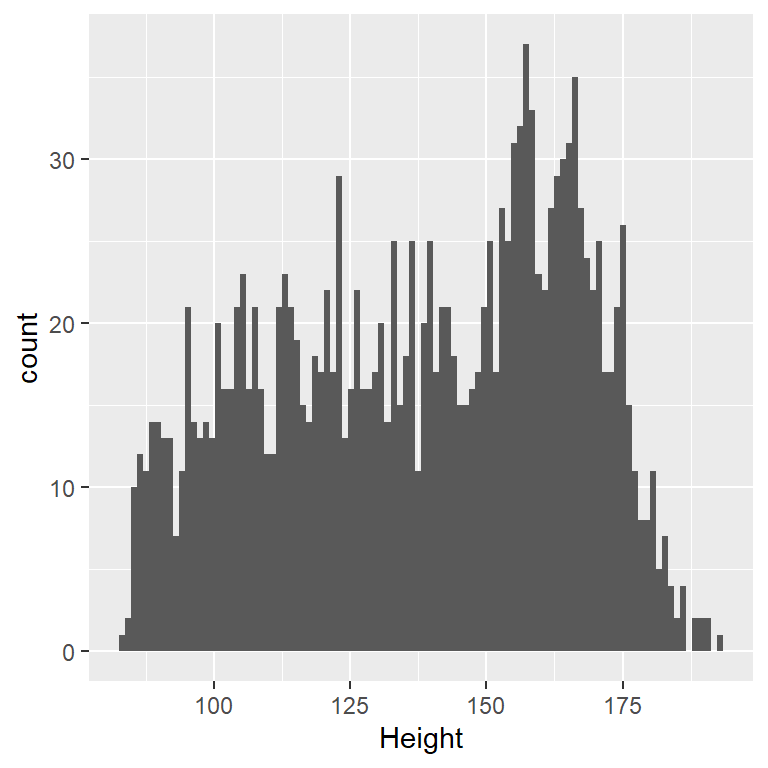
\includegraphics[height=0.5\textheight]{StatsThinking21_files/figure-latex/childHeight-1} \caption{Histogram of height of children in NHANES.}\label{fig:childHeight}
\end{figure}

Recuerda que queremos describir los datos de la forma más simple posible mientras que al mismo tiempo capturamos sus características más importantes. ¿Cuál es el modelo más simple que podemos imaginar que posiblemente aún captura la esencia de los datos? ¿Qué te parece el valor más común encontrado en el grupo de datos (el cual llamamos \emph{moda})?

Esto redefine el conjunto de 1691 niñxs en términos de un sólo número. Si quisiéramos predecir la altura de alguno de los nuevos niñxs, entonces nuestra estimación sería el mismo número: 166.5 centímetros.

\[
\hat{height_i} = 166.5
\]

Ponemos ese símbolo sobre el nombre de la variable para destacar que esta es nuestro valor \emph{predicho}. El error para este individuo sería entonces la diferencia entre el valor predicho (\(\hat{height_i}\)) y la altura real (\(height_i\)):

\[
error_i = height_i - \hat{height_i}
\]

¿Qué tan buen modelo es este? En general definimos qué tan bueno es un modelo en términos del error, el cual representa la diferencia entre el modelo y los datos; todas las cosas siendo iguales, el modelo que produce el error menor es el mejor modelo. (Aunque, como revisaremos más adelante, todas las cosas usualmente no son iguales\ldots).

Lo que encontramos es que la persona promedio tiene un margen de error algo grande de -28.8 centímetros comparado con la moda. Nos agradaría tener un modelo en donde el promedio de error es cero, y resulta ser que si utilizamos la media aritmética (comúnmente conocida como la \emph{media}) como nuestro modelo, entonces este será el caso.

La media (a menudo representada por una barra sobre la variable, como \(\bar{X}\)) es la suma de todos los valores, divididos entre el número de valores. Matemáticamente, expresamos esto como:

\[
\bar{X} = \frac{\sum_{i=1}^{n}x_i}{n}
\]

Podemos probar matemáticamente que la suma de los errores de la media (y por lo tanto, el promedio de error) es cero (mira la prueba al final de este capítulo si estás interesadx). Dado que el error promedio es cero, este parece ser el mejor modelo.

\begin{figure}
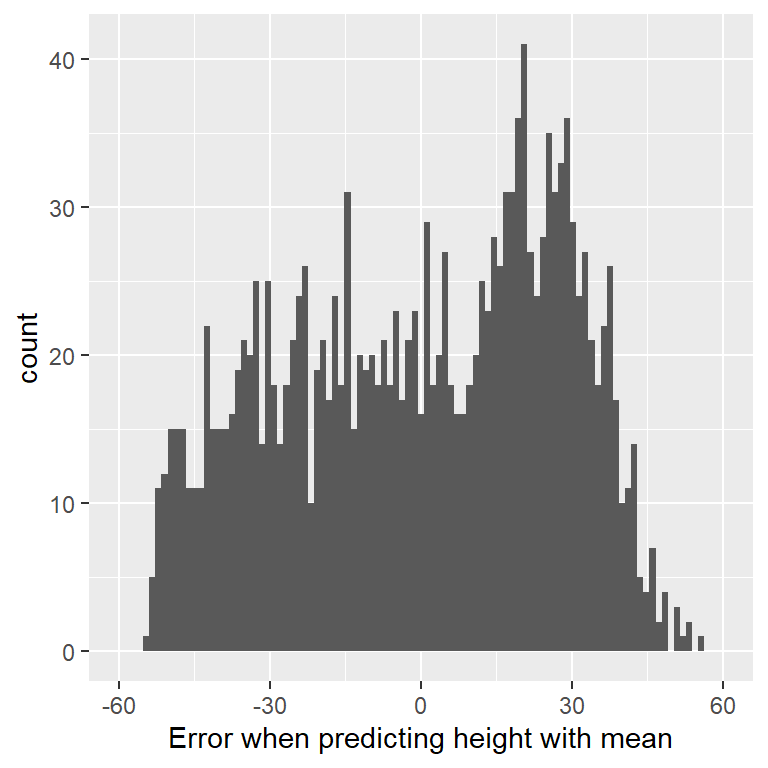
\includegraphics[height=0.5\textheight]{StatsThinking21_files/figure-latex/meanError-1} \caption{Distribution of errors from the mean.}\label{fig:meanError}
\end{figure}

A pesar de que el promedio de errores de la media es cero, podemos obsevar en el histograma en la Figura \ref{fig:meanError} que cada individuo aún tiene cierto grado de error; algunos son positivos y otros son negativos, y esos se cancelan entre ellos. Por esta razón, generalmente resumimos los errores en términos de algún tipo de medición que considera tanto los errores positivos como los negativos como malos. Podríamos usar el valor absoluto de cada error, pero es más común usar los errores al cuadrado, por razones que veremos después en el curso.

Existen varias formas comunes para resumir el error al cuadrado con el que te encontrarás en varios puntos de este libro, por lo que es importante comprender cómo se relacionan entre ellos. En primer instancia, podríamos simplemente sumarlos; esto se conoce como la \emph{suma de los errores al cuadrado} (\emph{sum of squared errors}). La razón por la que usualmente no utilizamos este método es porque su magnitud depende del número de datos, por lo que puede ser difícil de interpretar a menos que estemos viendo el mismo número de observaciones. En segundo lugar, podríamos tomar la media de los valores de error al cuadrado, lo cual se conoce como \emph{error cuadrático medio (MSE por sus siglas en inglés: mean squared error)}. Sin embargo, ya que elevamos al cuadrado los valores antes de promediarlos, no están en la misma escala que los datos originales; están en \(centímetros^2\). Por esta razón, también es común tomar la raíz cuadrada del \emph{error cuadrático medio}, al cual nos referimos como \emph{raíz del error cuadrático medio (RMSE por sus siglas en inglés: root mean squared error)}, para que el error sea medido en las mismas unidades que los valores originales (en este ejemplo, centímetros).

La media contiene una cantidad sustancial de error -- cualquier punto individual en los datos estará a unos 27 cm de la media en promedio -- pero aún así es mucho mejor que la moda, la cual tiene una raíz de error cuadrático medio de unos 39 cm.

\hypertarget{mejorando-nuestro-modelo}{%
\subsection{Mejorando nuestro modelo}\label{mejorando-nuestro-modelo}}

¿Podemos imaginar un mejor modelo? Recuerda que estos datos son de todxs lxs niñxs en la muestra NHANES, quienes varían de 2 a 17 años de edad. Dado este amplio rango de edades, esperaríamos que nuestro modelo de estatura también incluyera edad. Grafiquemos los datos de estatura frente a la edad, para ver si realmente existe relación.

\begin{figure}
\centering
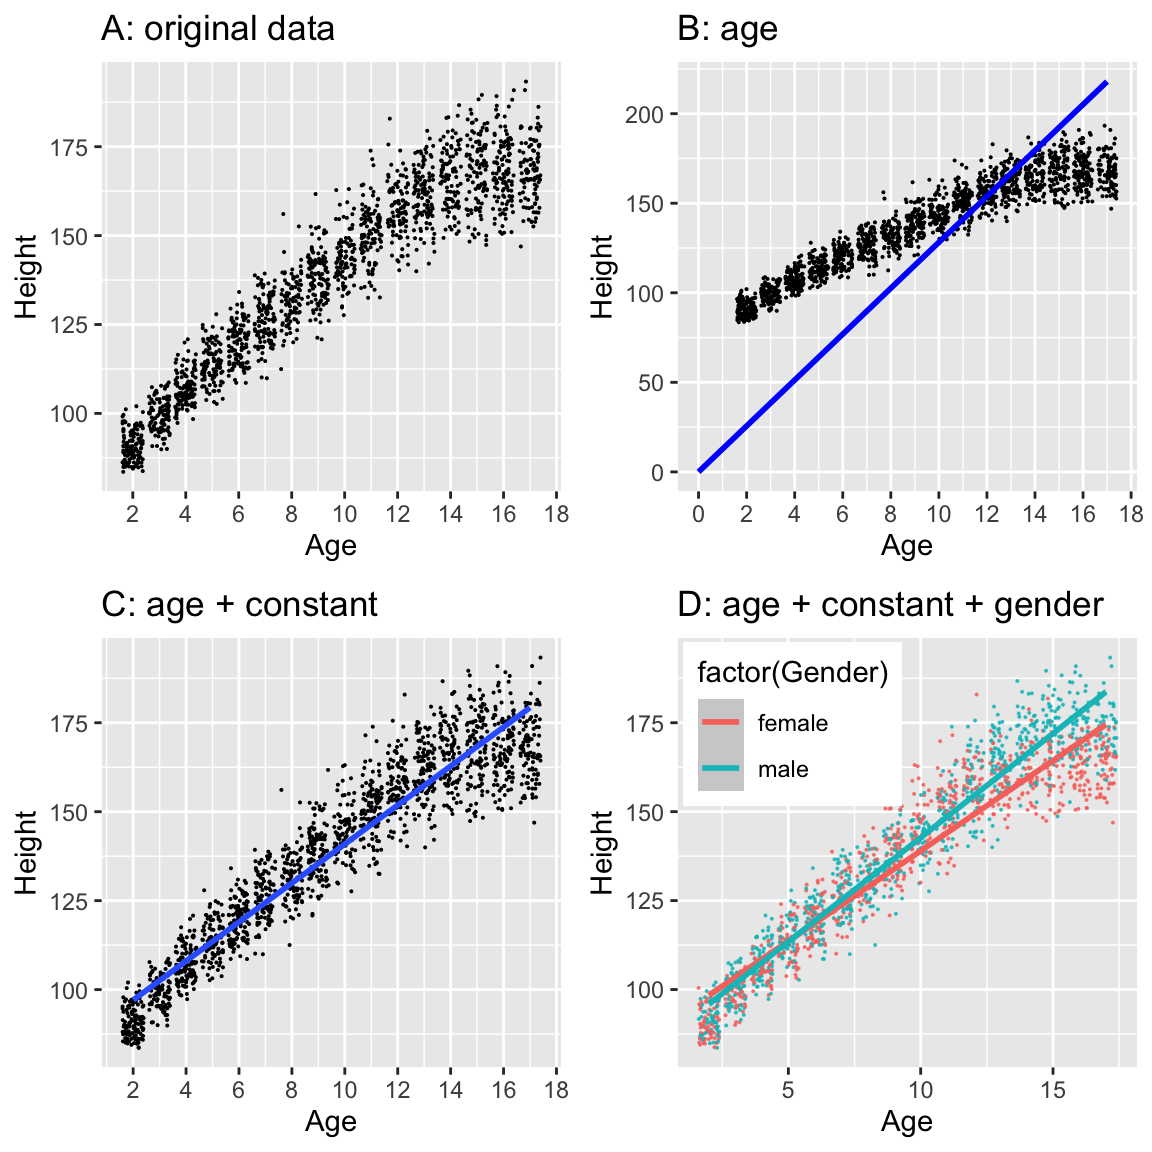
\includegraphics{StatsThinking21_files/figure-latex/childHeightLine-1.pdf}
\caption{\label{fig:childHeightLine}Height of children in NHANES, plotted without a model (A), with a linear model including only age (B) or age and a constant (C), and with a linear model that fits separate effects of age for males and females (D).}
\end{figure}

Los puntos negros en el Panel A de la Figura \ref{fig:childHeightLine} muestran individuos en el grupo de datos, y parece ser que hay una relación fuerte entre la edad y la estatura, como esperaríamos. Por lo que esperaríamos poder construir un modelo que relacione estatura y edad:

\[
\hat{height_i} =  \beta * age_i
\]

donde \(\beta\) es un \emph{parámetro} que multiplicamos por edad para obtener el error más pequeño.

Puede que recuerdes de álgebra que una línea se define de la siguiente manera:

\[
y = slope*x + intercept
\]

Si la edad es la variable \(X\), eso quiere decir que nuestra predicción de la altura conforme a la edad será una línea con una pendiente de \(\beta\) y una intercepción de cero. Para observar esto, tracemos una línea azul que mejor se acomode sobre los datos (Panel B en Figura \ref{fig:childHeightLine}). Algo está claramente mal con este modelo, ya que, la linea no parece seguir los datos muy bien. De hecho, ¡el RMSE para este modelo (39.16) es más alto que el modelo que solamente incluye la media! El problema radica en el hecho de que nuestro modelo solamente incluye la edad, lo cual significa que el valor de la altura predicho por el modelo debe tomar un valor de cero cuando la edad es cero. Aunque los datos no incluyen niñxs con edad de cero, la línea requiere matemáticamente tener un valor ``y'' de cero cuando ``X'' es cero, lo cual explica por qué la línea es jalada por debajo de los puntos de datos más bajos (o jóvenes). Podemos arreglar esto al incluir una intercepción (un \emph{intercepto}) en nuestro modelo, lo cual básicamente representa una altura estimada cuando la edad es igual a cero; aunque una edad de cero no es plausible en este conjunto de datos, este es un truco matemático que permitirá que el modelo tenga en cuenta la magnitud general de los datos.

\[
\hat{height_i} = intercept + \beta * age_i
\]

donde \emph{intercepto} (\emph{intercept}) es un valor constante agregado a la predicción para cada individuo; lo llamamos intercepto porque se mapea en la intersección en la ecuación de la línea recta. Más adelante aprenderemos cómo es que realmente calculamos estos valores de parámetros para un conjunto de datos en particular; por ahora, usaremos nuestro software estadístico para calcular los valores de la constante y de \(\beta\) que nos den el error más pequeño para este conjunto de datos en particular. El Panel C en la Figura \ref{fig:childHeightLine} muestra este modelo aplicado a los datos de NHANES, en donde podemos observar que la línea coincide con los datos mucho mejor que la que no tiene constante.

Nuestro error es mucho más pequeño utilizando este modelo -- sólo 8.36 centímetros en promedio. ¿Puedes pensar en otras variables que también se relacionen con la estatura? ¿Qué hay del género? En el Panel D de la Figura \ref{fig:childHeightLine} graficamos los datos con líneas distintas para género masculino y femenino. Observando sólo la gráfica, parece ser que existe una diferencia entre género masculino y femenino, pero es relativamente pequeño y solamente comienza después de la etapa de la pubertad. Estimemos este modelo y veamos cómo se ven los errores. En la Figura \ref{fig:msePlot} trazamos los valores de la raíz del error cuadrático medio a través de los diferentes modelos. Aquí podemos ver que el modelo mejoró un poco al pasar de moda a media, posteriormente mejora más al pasar de media a media + edad, y mejora sólo un poco más al incluir el género también.

\begin{figure}
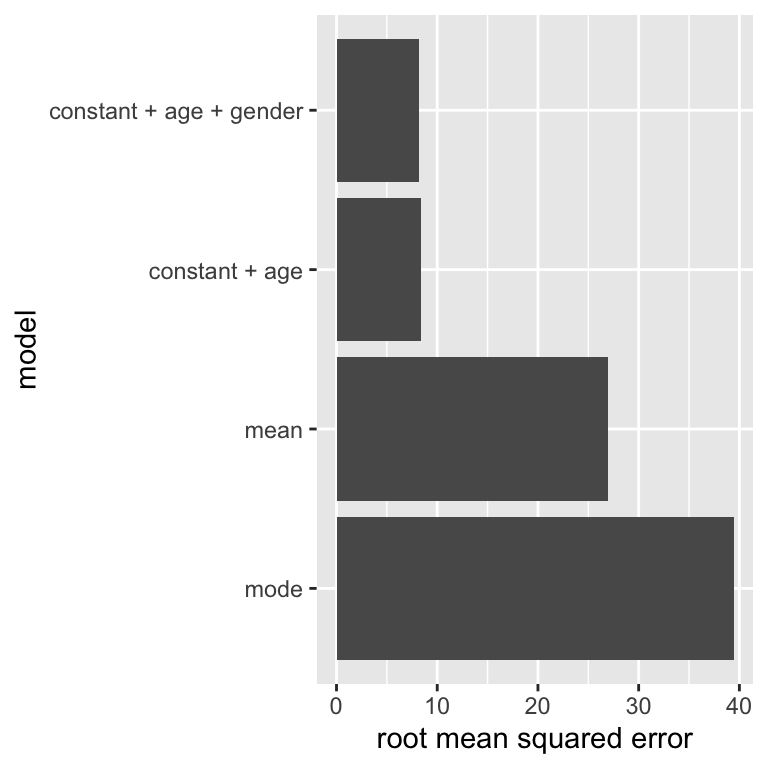
\includegraphics[height=0.5\textheight]{StatsThinking21_files/figure-latex/msePlot-1} \caption{Mean squared error plotted for each of the models tested above.}\label{fig:msePlot}
\end{figure}

\hypertarget{quuxe9-hace-que-un-modelo-sea-bueno}{%
\section{¿Qué hace que un modelo sea ``bueno''?}\label{quuxe9-hace-que-un-modelo-sea-bueno}}

Generalmente hay dos cosas diferentes que queremos de nuestro modelo estadístico. En primer lugar, queremos que describa nuestros datos correctamente; es decir, queremos que tenga el menor error posible cuando modelemos nuestros datos. En segundo lugar, queremos que se generalice bien a nuevas agrupaciones de datos; es decir, queremos que su error sea lo más bajo posible cuando lo apliquemos a una nueva agrupación de datos para poder hacer una predicción. Resulta ser que estas dos características se encuentran en conflicto constantemente.

Para entender esto, pensemos de dónde viene el error. Puede ocurrir si nuestro modelo está mal, por ejemplo, si de manera incorrecta afirmáramos que la altura declina conforme unx va creciendo en edad, en lugar de decir que la altura crece conforme a unx va cumpliendo más años. En este caso, nuestro error será mucho mayor de lo que sería con el modelo correcto. Similarmente, si hay un factor importante que le hace falta a nuestro modelo, esto también aumentará nuestro error (como ocurrió cuando dejamos de lado la edad para el modelo que generamos para la altura). De cualquier forma, un error también puede ocurrir cuando el modelo es correcto, debido a una posible variación aleatoria en los datos, a la cual solemos referirnos como ``error de medición'' o ``ruido''. A veces esto se debe a un error en nuestra medición -- por ejemplo, cuando la medición está bajo el cargo de unx humanx, al usar un cronómetro para medir tiempo transcurrido en una carrera a pie. En otros casos nuestra herramienta de medición puede ser muy exacta (como una escala digital para calcular el peso corporal), pero aquello que está siendo medido puede ser afectado por diversos factores que hacen que varíe. Si conociéramos todos estos factores, entonces podríamos generar un modelo más exacto, pero la realidad es que eso es raramente posible.

Usemos un ejemplo para ilustrar esto. En lugar de utilizar datos reales, generaremos datos para este ejemplo utilizando una simulación por computadora (de la cual hablaremos más adelante en los siguientes capítulos). Digamos que queremos comprender la relación entre el contenido de alcohol en la sangre (``BAC'' por sus siglas en inglés: \emph{blood alcohol content}) y su tiempo de reacción en una prueba de conducir simulada. Podemos generar algunos datos simulados y graficar la relación (ver Panel A de la Figura \ref{fig:BACrt}).

\begin{figure}
\centering
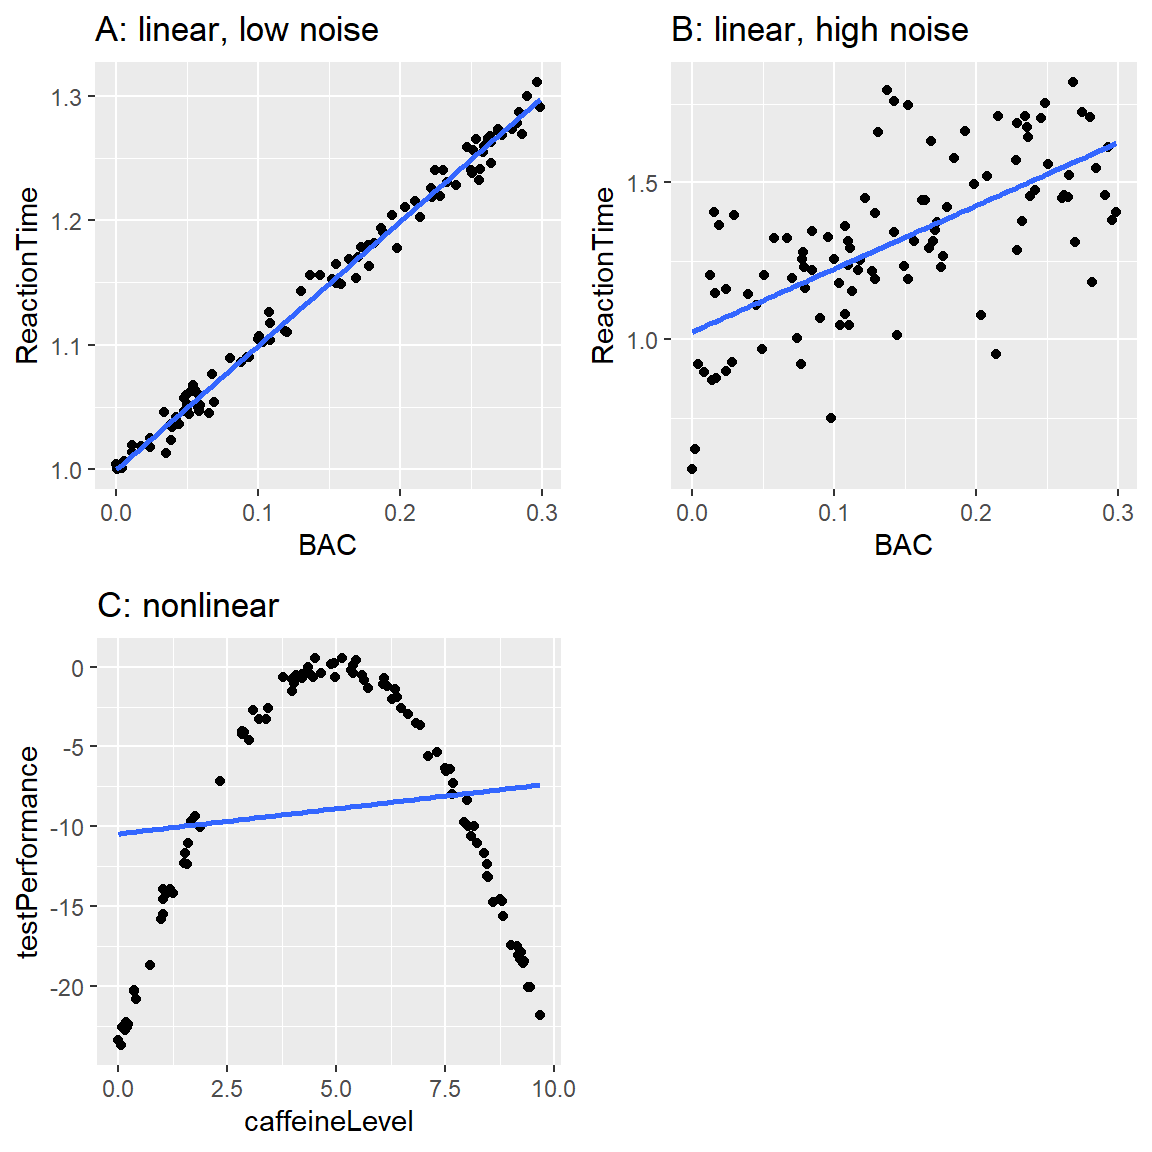
\includegraphics{StatsThinking21_files/figure-latex/BACrt-1.pdf}
\caption{\label{fig:BACrt}Simulated relationship between blood alcohol content and reaction time on a driving test, with best-fitting linear model represented by the line. A: linear relationship with low measurement error. B: linear relationship with higher measurement error. C: Nonlinear relationship with low measurement error and (incorrect) linear model}
\end{figure}

En este ejemplo, el tiempo de reacción sube sistemáticamente con el contenido de alcohol en la sangre -- la línea muestra el modelo más adecuado, y podemos ver que hay un margen de error pequeño, el cual se evidencia en el hecho de que todos los puntos están muy cerca de la línea.

También podemos pensar en datos que muestren la misma relación linear, pero que tengan un mayor margen de error, como en el Panel B de la Figura \ref{fig:BACrt}. Aquí podemos ver que aún hay un incremento sistemático del tiempo de reacción con el contenido de alcohol en la sangre (BAC), pero es mucho más variable a lo largo de lxs individuos.

Estos fueron dos ejemplos en donde el \emph{modelo lineal} parece apropiado, y el error refleja ruido en nuestra medición. El modelo lineal especifica que la relación entre dos variables sigue una línea recta. Por ejemplo, en un modelo lineal, un incremento particular en el contenido de alcohol en la sangre (BAC) siempre es asociado con un aumento específico en el tiempo de reacción, independientemente del nivel de contenido de alcohol en la sangre (BAC).

Por otro lado, hay situaciones en donde el modelo lineal es incorrecto, y el error va a incrementar porque el modelo no está correctamente especificado. Digamos que estamos interesadxs en la relación entre la ingesta de cafeína y el rendimiento en un examen. La relación entre estimulantes como la cafeína y el rendimiento en un examen es a menudo \emph{no lineal} - esto quiere decir que no sigue una línea recta. Esto es porque el rendimiento sube con cantidades pequeñas de cafeína (conforme la persona se pone más alerta), pero después empieza a declinar con cantidades grandes (conforme la persona se pone más nerviosa). Podemos simular datos de esta forma, y luego ajustar un modelo lineal a los datos (observa el Panel C de la Figura \ref{fig:BACrt}). La línea azul muestra una línea recta que mejor se ajusta a estos datos; claramente, hay un alto margen de error. Aunque existe una relación entre el rendimiento de la prueba y la ingesta de cafeína, sigue a una curva en lugar de a una línea recta. El modelo lineal tiene mayor error porque es el modelo incorrecto para este tipo de datos.

\hypertarget{overfitting}{%
\section{¿Un modelo puede ser demasiado bueno?}\label{overfitting}}

Un error suena como algo malo, y usualmente vamos a preferir un modelo que tenga menor error a uno que tenga mayor error. No obstante, ya mencionamos que existe tensión entre la habilidad de un modelo para ajustarse correctamente a un conjunto de datos en particular y su habilidad para generalizarse a nuevos conjuntos de datos\ldots{} ¡Y resulta ser que el modelo con el menor error es a menudo peor para generalizarse a nuevos conjuntos de datos!

Para ver esto, hay que generar de nuevo un conjunto de datos para que podamos conocer la verdadera relación entre las variables. Crearemos dos conjuntos de datos simulados, los cuales se generarán de la misma manera exacta -- solamente que van a tener diferente ruido aleatorio añadido a ellos.

\begin{figure}
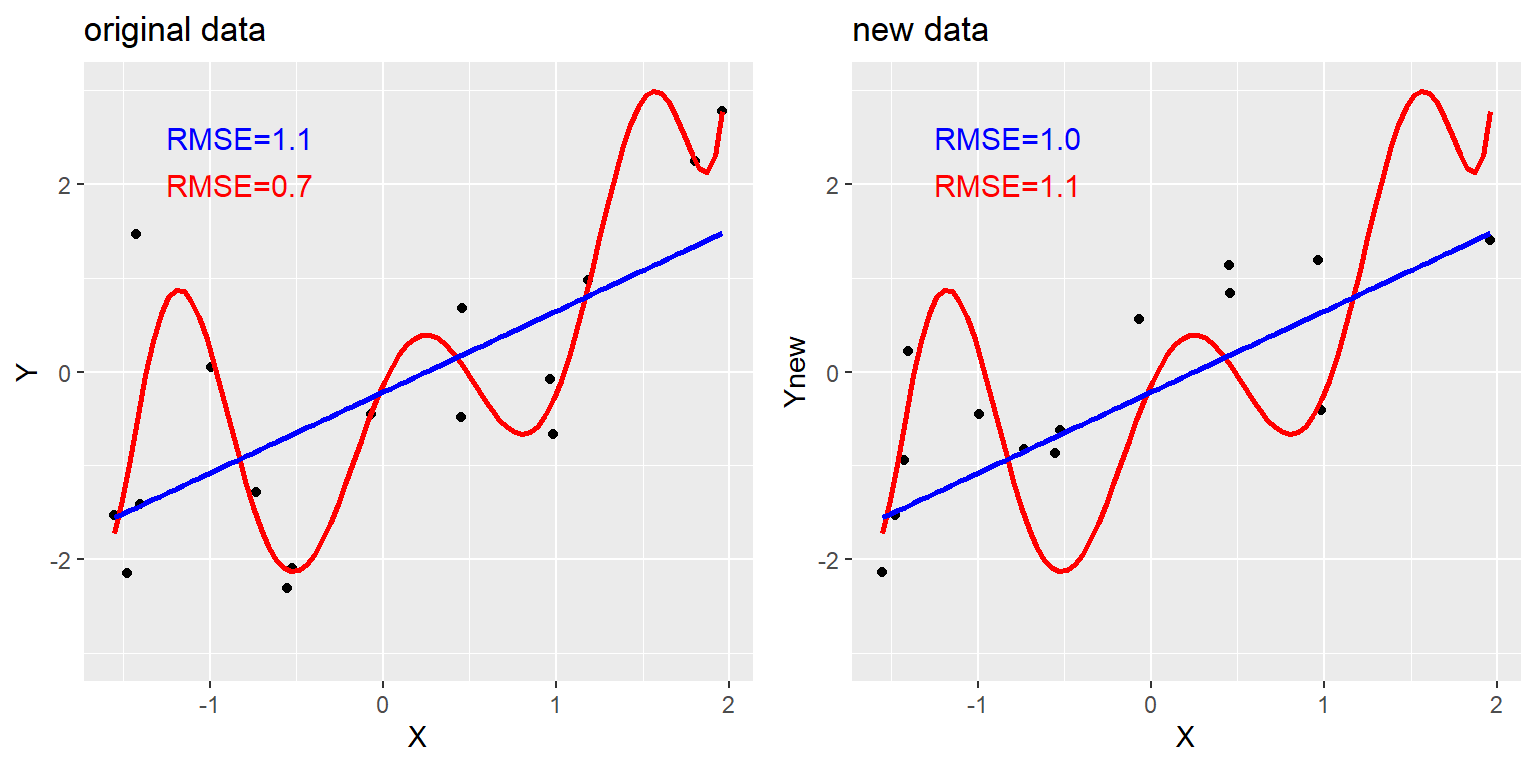
\includegraphics[height=0.5\textheight]{StatsThinking21_files/figure-latex/Overfitting-1} \caption{An example of overfitting. Both datasets were generated using the same model, with different random noise added to generate each set.  The left panel shows the data used to fit the model, with a simple linear fit in blue and a complex (8th order polynomial) fit in red.  The root mean square error (RMSE) values for each model are shown in the figure; in this case, the complex model has a lower RMSE than the simple model.  The right panel shows the second dataset, with the same model overlaid on it and the RMSE values computed using the model obtained from the first dataset.  Here we see that the simpler model actually fits the new dataset better than the more complex model, which was overfitted to the first dataset.}\label{fig:Overfitting}
\end{figure}

El panel de la izquierda en la Figura \ref{fig:Overfitting} muestra que el modelo más complejo (en rojo) se ajusta a los datos mejor que el modelo simple (en azul) generado en la misma manera-- aquí podemos observar que el modelo más simple se ajusta mejor al nuevo conjunto de datos que el modelo complejo. Intuitivamente podemos observar que el modelo complejo está influenciado por los puntos specíficos de los datos en el primer conjunto de datos; dado que la posición exacta de estos puntos de datos fue impulsada por ruido aleatorio, esto lleva al modelo complejo a ajustarse mal en el nuevo conjunto de datos. A este fenómeno lo llamamos \emph{sobreajuste} (\emph{overfitting} en inglés). Por ahora es importante que mantengamos en mente que nuestro modelo debe ajustarse bien, pero no demasiado bien. Como lo dijo alguna vez Albert Einstein (1933): ``Difícilmente se puede negar que el fin supremo de toda teoría es hacer que los elementos básicos irreductibles sean lo más simples y pocos posibles sin tener que renunciar a la representación adecuada de un solo dato de experiencia.'' Lo cual se parafrasea a: ``Todo debe de ser tan simple como pueda ser, pero no más simple.''

\hypertarget{el-modelo-muxe1s-simple-la-media}{%
\section{El modelo más simple: La media}\label{el-modelo-muxe1s-simple-la-media}}

Ya nos hemos encontrado con la media (o promedio), y de hecho, la mayoría de las personas conoce qué es un promedio, incluso si nunca han tomado una clase de estadística. Es más comunmente usado para describir lo que llamamos la ``tendencia central'' del conjunto de datos -- ¿cuál es el valor en el que se centran los datos? La mayoría de las personas no piensa que calcular una media es ajustar un modelo a los datos. Sin embargo, eso es exactamente lo que estamos haciendo cuando calculamos la media.

Ya hemos revisado la formula para calcular la media de una muestra de datos:

\[
\bar{X} = \frac{\sum_{i=1}^{n}x_i}{n}
\]

Nota que dije que esta fórmula es específica para una \emph{muestra} de datos, lo cual es un grupo de datos seleccionados de una población más grande. Usando una muestra, deseamos caracterizar una población más grande -- el conjunto total de individuos en lxs que estamos interesadxs. Por ejemplo, si fuéramos unx encuestadxr político nuestra población de interés tal vez serían todxs lxs votantes registradxs, mientras que nuestra muestra podría incluir solo unos pocos miles de personas de esta población. Más adelante en este curso estaremos hablando con más detalle sobre el muestreo, pero por ahora el punto importante es que a lxs estadísticxs generalmente les gusta usar diferentes símbolos para diferenciar \emph{estadísticas} que describen valores para una muestra de \emph{parámetros} que describen los valores verdaderos para una población; en este caso la fórmula para la media (denotada como \(\mu\)) de la población es:

\[
\mu = \frac{\sum_{i=1}^{N}x_i}{N}
\]

donde N es el tamaño de la población completa.

Ya hemos visto que la media es el resumen estadístico que nos garantiza darnos un error promedio de cero. La media también tiene otra característica: es el resumen estadístico que tiene el valor más bajo posible para la suma de errores cuadráticos (SSE, \emph{sum of squared errors}). En estadística, nos referimos a esto como el ``mejor'' estimador . Podríamos probarlo matemáticamente, pero en su lugar vamos a demostrarlo gráficamente en la Figura \ref{fig:MinSSE}.

\begin{figure}
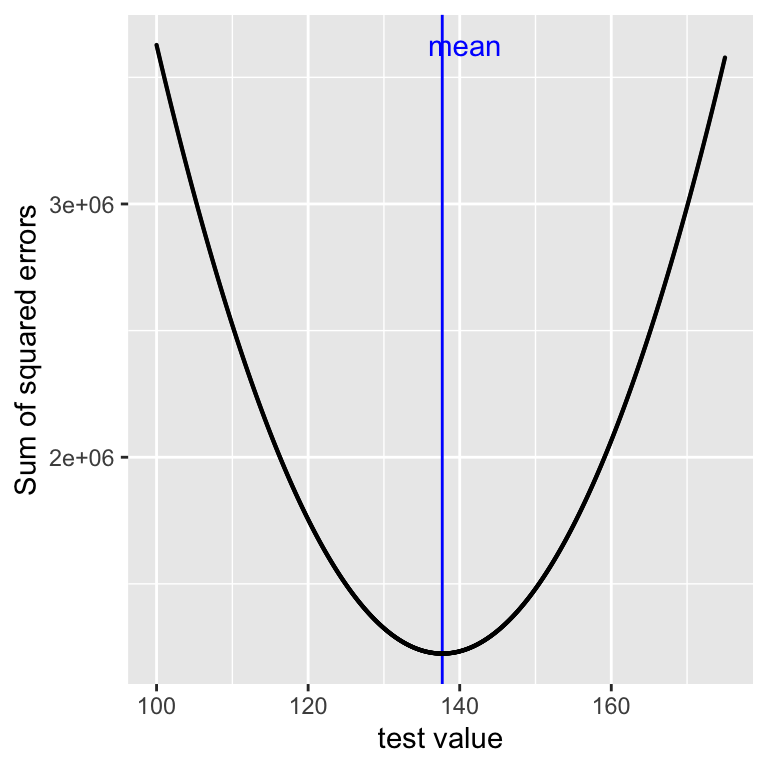
\includegraphics[height=0.5\textheight]{StatsThinking21_files/figure-latex/MinSSE-1} \caption{Una demostración de la media como la estadística que minimiza la suma de los errores cuadráticos. Utilizando los datos de la altura del NHANES, calculamos la media (la barra azul). Luego, probamos un rango de otros valores, y por cada uno calculamos la suma de errores cuadráticos por cada dato de ese valor, el cual se indica por la curva negra. Vemos que la media cae al mínimo en la gráfica del error cuadrático.}\label{fig:MinSSE}
\end{figure}

El minimizar la suma de los errores cuadráticos (SSE) es una buena característica, y es la razón por la que la media es el estadístico más comunmente usado para resumir datos. No obstante, la media también tiene su lado oscuro. Digamos que hay cinco personas en un bar, y examinamos el ingreso económico de cada unx:

\begin{table}

\caption{\label{tab:unnamed-chunk-17}Income for our five bar patrons}
\centering
\begin{tabular}[t]{r|l}
\hline
income & person\\
\hline
48000 & Joe\\
\hline
64000 & Karen\\
\hline
58000 & Mark\\
\hline
72000 & Andrea\\
\hline
66000 & Pat\\
\hline
\end{tabular}
\end{table}

La media (61600.00) parece ser una buena herramienta para medir el ingreso económico de esas cinco personas. Ahora observemos lo que pasa cuando Beyoncé Knowles entra al bar (además de la emoción de todxs):

\begin{table}

\caption{\label{tab:unnamed-chunk-19}Income for our five bar patrons plus Beyoncé Knowles.}
\centering
\begin{tabular}[t]{l|l}
\hline
income & person\\
\hline
48000 & Joe\\
\hline
64000 & Karen\\
\hline
58000 & Mark\\
\hline
72000 & Andrea\\
\hline
66000 & Pat\\
\hline
54000000 & Beyonce\\
\hline
\end{tabular}
\end{table}

La media es ahora casi 10 millones de dólares, lo cual no es verdaderamente representativo de lo que ganan las primeras cinco personas que estaban en el bar -- en particular, la media está altamente influenciada por el valor extremo de Beyoncé. En general, la media es altamente sensible a valores extremos. Es por eso que siempre es importante asegurarnos de que no haya valores extremos cuando utilicemos la media para resumir datos.

\hypertarget{la-mediana}{%
\subsection{La mediana}\label{la-mediana}}

Si queremos resumir los datos en una forma que sea menos sensible a valores atípicos, podemos utilizar otra herramienta estadística llamada la \emph{mediana}. Si nuestro propósito fuera acomodar todos los valores en orden de su magnitud, entonces la mediana es el valor que queda en medio. Si hay un número par de valores, entonces habrá dos valores empatados para el lugar medio, en cuyo caso tomamos la media (es decir, el punto medio) de esos dos números.

Veamos un ejemplo: Digamos que queremos resumir los siguientes valores:

\begin{verbatim}
8  6  3 14 12  7  6  4  9
\end{verbatim}

Si ordenamos dichos valores:

\begin{verbatim}
3  4  6  6  7  8  9 12 14
\end{verbatim}

Entonces la mediana es el valor de en medio -- en este caso, el quinto de los nueve valores.

Mientras que la media minimiza la suma de los errores cuadráticos, la mediana minimiza una cantidad ligeramente distinta: la suma de los errores \emph{absolutos} (absolute errors). Esto explica por qué es menos sensible a valores atípicos -- elevar al cuadrado va a exacerbar el efecto de errores grandes en comparación con tomar el valor absoluto. Podemos ver esto en el caso del ingreso económico: la mediana es mucho más representativa de todo el grupo, y menos sensible a un valor atípico.

\begin{table}

\caption{\label{tab:unnamed-chunk-20}Summary statistics for income after arrival of Beyoncé Knowles.}
\centering
\begin{tabular}[t]{l|r}
\hline
Statistic & Value\\
\hline
Mean & 9051333\\
\hline
Median & 65000\\
\hline
\end{tabular}
\end{table}

Dado esto, ¿por qué utilizaríamos entonces la media? Como veremos más adelante en este capítulo, la media es el ``mejor'' estimador en el sentido de que varía menos de muestra en muestra en comparación con otros estimadores. Queda en nosotrxs decidir si vale la pena su sensibilidad a posibles valores atípicos -- la estadística se trata de balancear ventajas y desventajas.

\hypertarget{la-moda}{%
\section{La moda}\label{la-moda}}

A veces deseamos describir la tendencia central de un conjunto de datos que no es numérico. Por ejemplo, digamos que queremos saber cuáles modelos de iPhones son más comunmente usados. Para probar esto, podemos preguntarle a un grupo grande de usuarios de iPhone cuál modelo es el que cada unx tiene. Si sacáramos el promedio de esos valores posiblemente veamos que la media del modelo de iPhone sería 9.51, lo cual no tiene sentido, ya que, el número de modelo de iPhone no están diseñados para ser mediciones cuantitativas. En este caso, una medición de tendencia central más apropiada es la moda, cuál es el valor más común en el conjunto de datos.

\hypertarget{variabilidad-quuxe9-tan-bien-se-ajusta-la-media-a-los-datos}{%
\section{Variabilidad: ¿Qué tan bien se ajusta la media a los datos?}\label{variabilidad-quuxe9-tan-bien-se-ajusta-la-media-a-los-datos}}

Una vez que hemos descrito la tendencia central de los datos, a menudo también vamos a querer describir qué tan variables son los datos -- a esto se le refiere también como ``dispersión'', reflejando el hecho de que describe qué tan dispersos están los datos.

Ya hemos encontrado la suma de errores cuadráticos arriba, lo cual es la base para las mediciones más comunmente usadas para la variablidad: la \emph{varianza} y la \emph{desviación estándar}. La varianza para una población (referida como \(\sigma^2\)) es simplemente la suma de los errores cuadráticos divididos entre el número de observaciones-- lo cual es exactamente lo mismo que el \emph{error cuadrático medio} del que hablamos hace poco:

\[
\sigma^2 = \frac{SSE}{N} = \frac{\sum_{i=1}^n (x_i - \mu)^2}{N}
\]

donde \(\mu\) es la media de la población. La desviación estándar es simplemente la raíz cuadrada de esto -- es la \emph{raíz del error cuadrático medio} que vimos antes. La desviación estándar es útil porque los errores están en las mismas unidades que en los datos originales (al deshacer el cuadrado que aplicamos a los errores).

Usualmente no tenemos acceso a toda la población, por lo que debemos calcular la varianza utilizando una muestra, a la cual nos referimos como \(\hat{\sigma}^2\), con el ``sombrero'' representando el hecho de que es un estimado basado en una muestra. La ecuación para \(\hat{\sigma}^2\) es similar a la de \(\sigma^2\):

\[
\hat{\sigma}^2 = \frac{\sum_{i=1}^N (x_i - \bar{X})^2}{n-1}
\]

La única diferencia entre las dos ecuaciones es que dividimos entre \(n - 1\) en lugar de \(N\). Esto se relaciona con un concepto estadístico fundamental: \emph{grados de libertad}. Recuerda que para calcular la varianza de la muestra, primero tuvimos que estimar la media de la muestra \(\bar{X}\). Al haber estimado esto, un valor en los datos ya no puede variar libremente. Por ejemplo, digamos que tenemos los siguientes datos para una variable \(x\): {[}3, 5, 7, 9, 11{]}, la media es 7. Porque sabemos que la media de este conjunto de datos es 7, podemos calcular cuál sería cualquier valor específico si faltara. Por ejemplo, digamos que ocultamos el primer valor (3). Al hacer esto, aún sabemos que su valor debe de ser 3, porque la media de 7 implica que la suma de todos los valores es \(7 * n = 35\) y \(35 - (5 + 7 + 9 + 11) = 3\).

Entonces, cuando decimos que hemos ``perdido'' un grado de libertad, quiere decir que hay un valor que no puede variar libremente después de haberse acomodado al modelo. En el contexto de la varianza de la muestra, si no contemplamos la pérdida de grados de libertad, entonces nuestra estimación de la varianza de la muestra estará \emph{sesgada}, ocasionando que subestimemos la incertidumbre de nuestra estimación de la media.

\hypertarget{usar-simulaciones-para-entender-la-estaduxedstica}{%
\section{Usar simulaciones para entender la estadística}\label{usar-simulaciones-para-entender-la-estaduxedstica}}

Soy un ávido creyente en el uso de simulaciones en computadora para comprender conceptos de estadística, y en capítulos futuros ahondaremos más en su uso. Aquí les presentaré la idea preguntándoles si podemos confirmar la necesidad de restar 1 del tamaño de la muestra al calcular la varianza de la muestra.

Usemos la muestra completa de los datos de lxs niñxs de NHANES como nuestra ``población'', y observemos qué tan bien los cálculos de la varianza de la muestra utilizando tanto \(n\) como \(n-1\) en el denominador estimará la varianza de esta población a lo largo de un gran número de muestras simuladas aleatorias obtenidas del conjunto de datos. Regresaremos a los detalles de cómo se hace esto en un capítulo próximo.

\begin{table}

\caption{\label{tab:unnamed-chunk-22}Variance estimates using n versus n-1; the estimate using n-1 is closer to the population value}
\centering
\begin{tabular}[t]{l|r}
\hline
Estimate & Value\\
\hline
Population variance & 725\\
\hline
Variance estimate using n & 710\\
\hline
Variance estimate using n-1 & 725\\
\hline
\end{tabular}
\end{table}

Esto nos demuestra que la teoría propuesta arriba era correcta: la varianza estimada utilizando \(n - 1\) como el denominador se acerca mucho a la varianza calculada con todos los datos (la población), por lo que la varianza calculada utilizando \(n\) como el denominador está sesgada en comparación con el valor real.

\hypertarget{puntajes-z}{%
\section{Puntajes Z}\label{puntajes-z}}

Habiendo caracterizado una distribución en términos de su tendencia central y su variabilidad, a menudo es útil expresar los puntajes individuales en términos de en dónde se ubican con respecto a la distribución total. Digamos que estamos interesadxs en determinar si California es un lugar particularmente peligroso. Podemos responder a esta pregunta utilizando datos del 2014 del {[}FBI's Uniform Crime Reporting Site{]} (\url{https://www.ucrdatatool.gov/Search/Crime/State/RunCrimeOneYearofData.cfm}).
El panel de la izquierda de la Figura \ref{fig:crimeHist} muestra un histograma del número de crímenes violentos por estado, resaltando el valor de California. Observando estos datos, parece que California es terriblemente peligroso, con 153709 crímenes en ese año.

Podemos visualizar estos datos al generar un mapa mostrando una distribución de la variable a lo largo de los estados, el cual se presenta en el panel de la derecha de la Figura \ref{fig:crimeHist}.

\begin{figure}
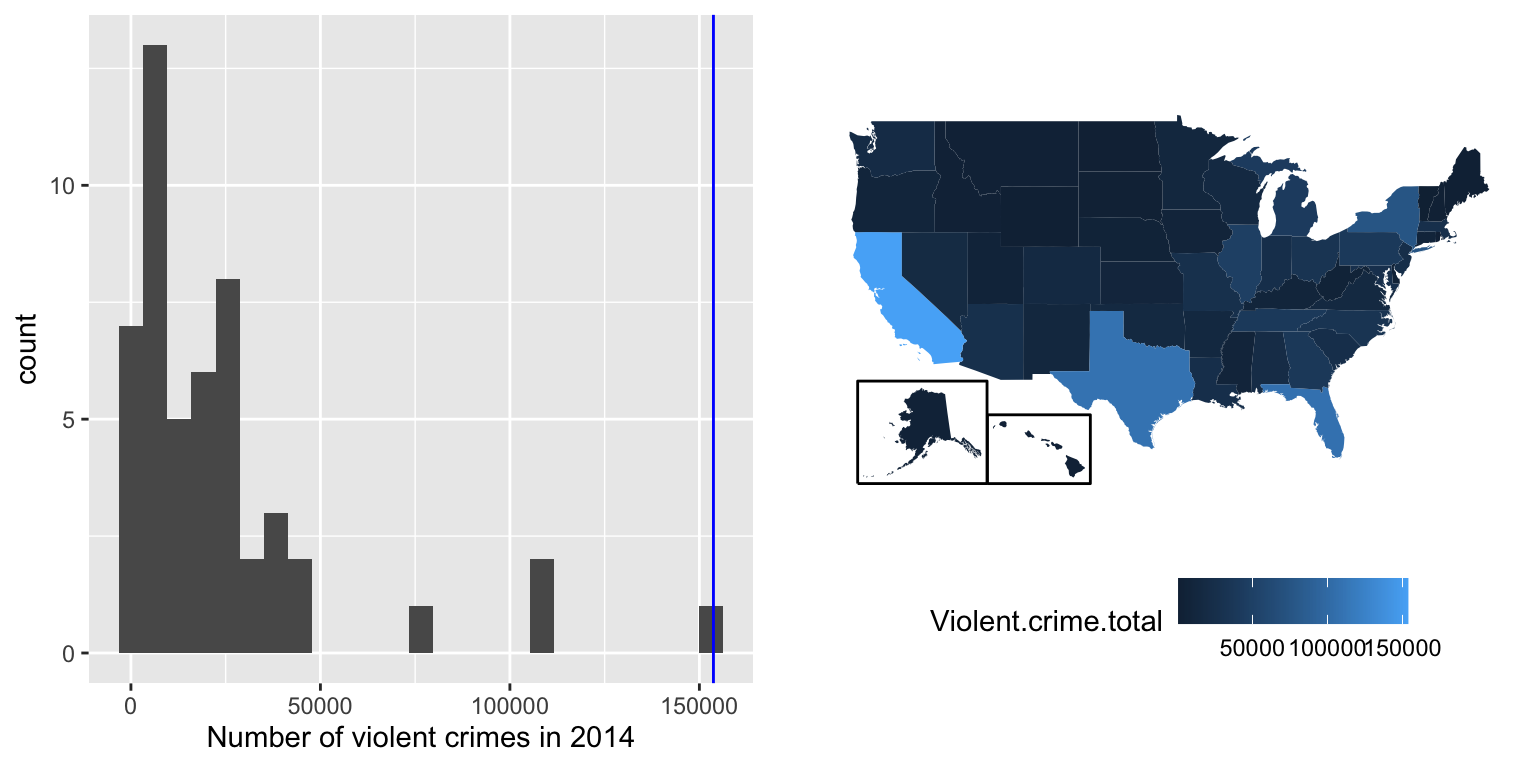
\includegraphics[height=0.5\textheight]{StatsThinking21_files/figure-latex/crimeHist-1} \caption{Left: Histogram of the number of violent crimes.  The value for CA is plotted in blue. Right: A map of the same data, with number of crimes plotted for each state in color.}\label{fig:crimeHist}
\end{figure}

Tal vez hayas notado que California también tiene la población más grande de cualquier estado en Estados Unidos, por lo que es razonable que también tenga un gran número de crímenes. Si graficamos los números de crímenes junto con la población de cada estado (ve el panel izquierdo de la Figura \ref{fig:popVsCrime}), vemos que hay una relación directa entre las dos variables.

\begin{figure}
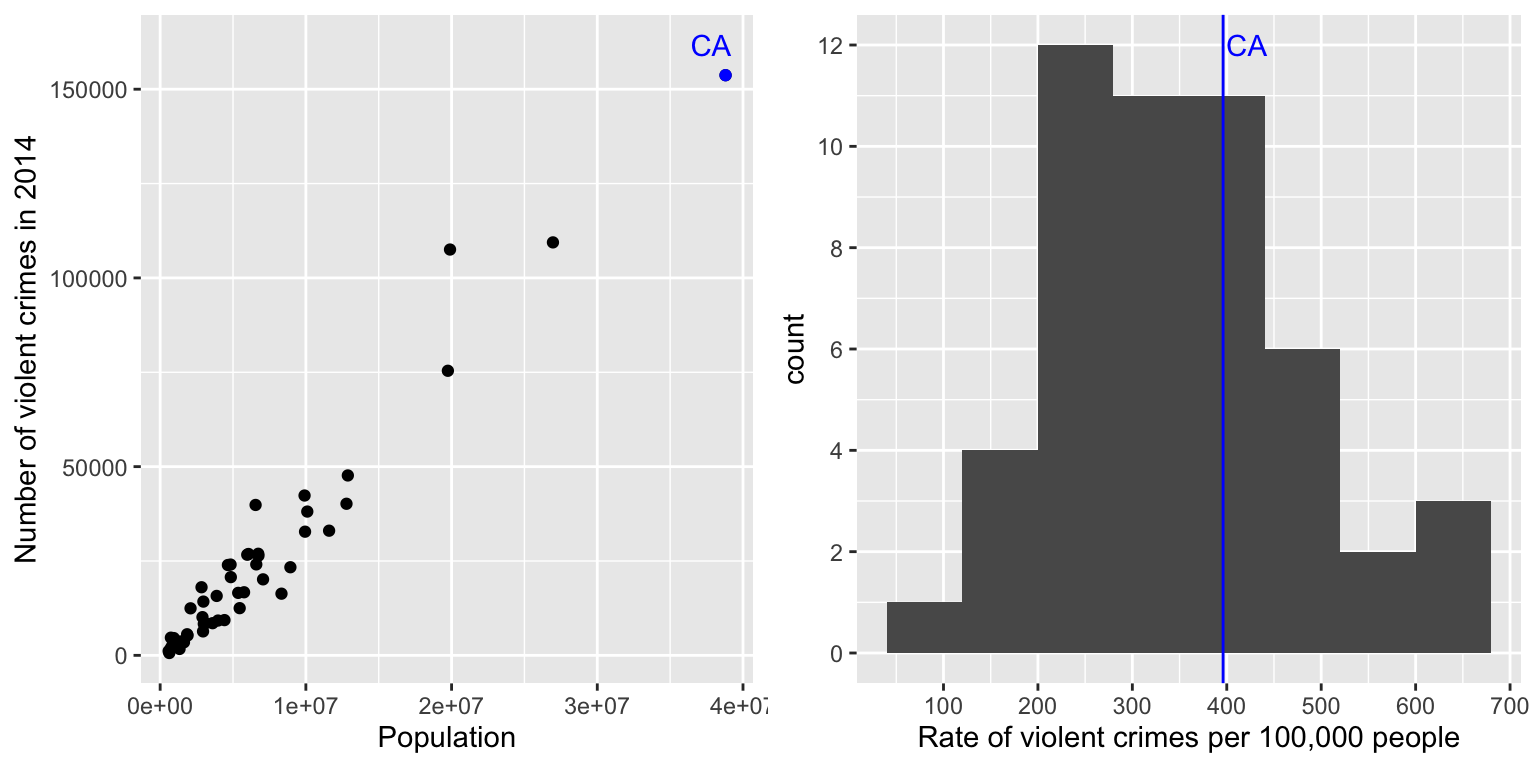
\includegraphics[height=0.5\textheight]{StatsThinking21_files/figure-latex/popVsCrime-1} \caption{Left: A plot of number of violent crimes versus population by state. Right: A histogram of per capita violent crime rates, expressed as crimes per 100,000 people.}\label{fig:popVsCrime}
\end{figure}

En lugar de utilizar los números en bruto (o crudos) para los crímenes, debemos usar la \emph{tasa} de crímenes violentos per cápita, el cual obtenemos al dividir el número de crímenes por estado entre la población de cada estado. El conjunto de datos del FBI ya incluye este valor (expresado como tasa por 100,000 habitantes). Observando el panel de la derecha de la Figura \ref{fig:popVsCrime}, podemos ver que California no es tan peligrosa después después de todo -- su tasa de crímenes es 396.10 por cada 100,000 habitantes está un poco por arriba de la media de los estados de 346.81, pero está dentro del rango de muchos otros estados. ¿Pero qué pasa si queremos obtener una vista más clara de qué tanto se aleja California del resto de la distribución?

El \emph{puntaje Z} (\emph{Z-score}) nos permite expresar datos en una forma que proporciona más información sobre cada punto de datos y su relación con el total de la distribución. La fórmula que calcula el puntaje Z para un dato invididual, dado que ya conocemos el valor de la media de la población \(\mu\) y su desviación estándar \(\sigma\) es:

\[
Z(x) = \frac{x - \mu}{\sigma}
\]

Intuitivamente, podemos pensar en un puntaje Z como un indicador que nos dice qué tan lejos está cada punto o dato individual en referencia con la media, en unidades de la desviación estándar. Podemos calcular esto para los datos de la tasa de crímenes, como se muestra en la Figura \ref{fig:crimeZplot}.

\begin{figure}
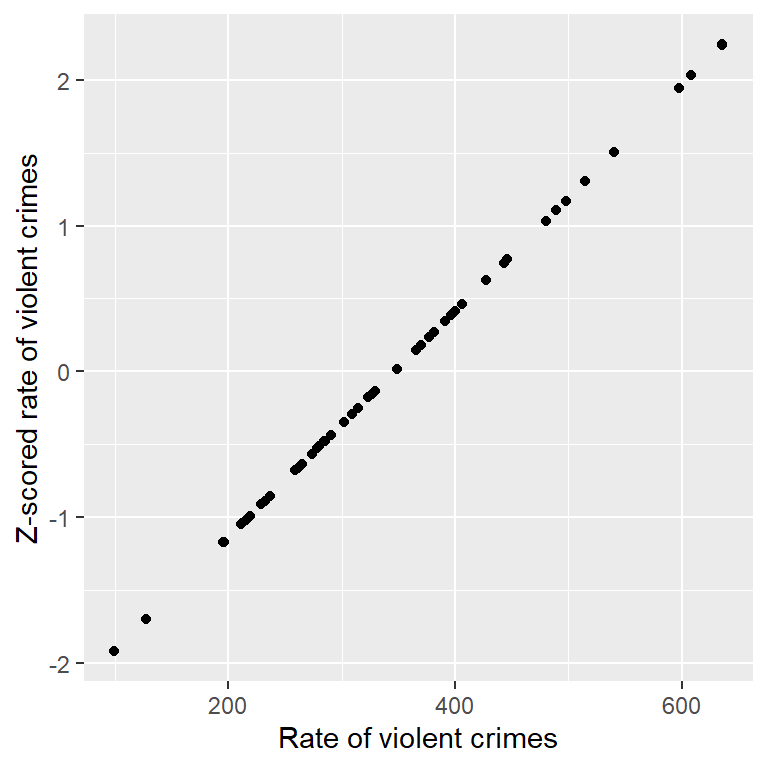
\includegraphics[height=0.5\textheight]{StatsThinking21_files/figure-latex/crimeZplot-1} \caption{Scatterplot of original crime rate data against Z-scored data.}\label{fig:crimeZplot}
\end{figure}

El diagrama de dispersión nos muestra que el proceso de sacar el puntaje Z no cambia la distribución relativa de los datos (esto es visible en el hecho de que los datos originales y el puntaje Z de los datos caen en una línea recta cuando se grafican una contra la otra).
Sólo las acomoda para que tengan una media de cero y una desviación estándar de uno. En la figura \ref{fig:crimeZmap} se muestran geográficamente los datos de crimen utilizando valores Z

\begin{figure}
\centering
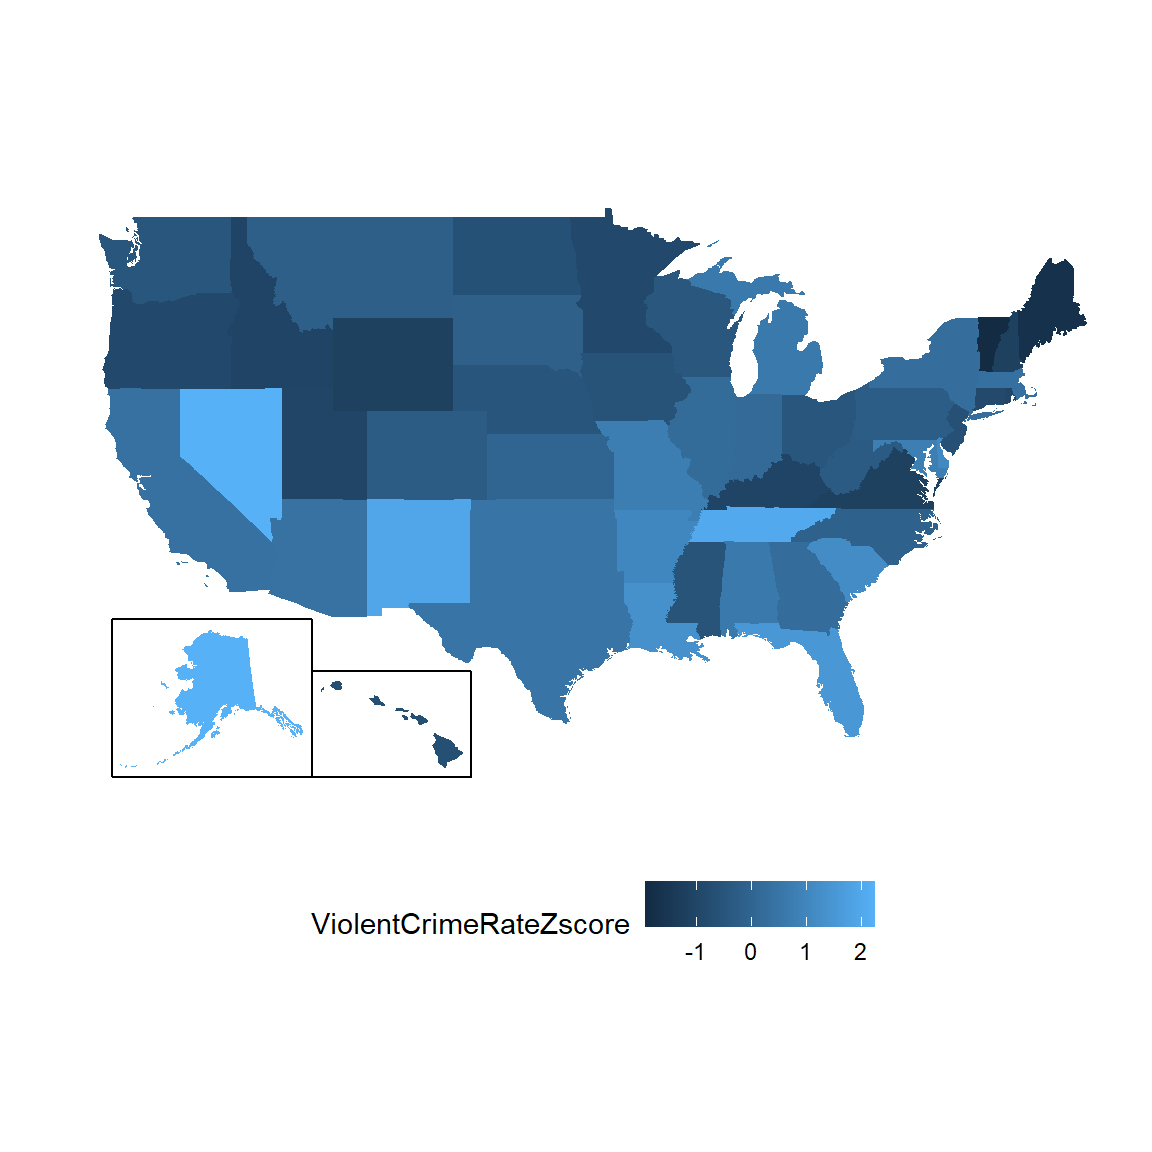
\includegraphics{StatsThinking21_files/figure-latex/crimeZmap-1.pdf}
\caption{\label{fig:crimeZmap}Crime data rendered onto a US map, presented as Z-scores.}
\end{figure}

Esto nos da una mirada un poco más interpretable de los datos. Por ejemplo, ahora podemos ver que Nevada, Tenessee y Nuevo México tienen tasas de crímenes que están aproximadamente dos desviaciones estándar por encima de la media.

\hypertarget{interpretando-puntajes-z}{%
\subsection{Interpretando Puntajes Z}\label{interpretando-puntajes-z}}

La ``Z'' en un ``puntaje Z'' proviene del hecho de que la distribución estándar normal (la distribución normal con una media de cero y una desviación estándar de 1) es a menudo referida como la distribución ``Z''. Podemos usar la distribución estándar normal para ayudarnos a comprender lo que los puntajes Z específicos nos dicen acerca de dónde se encuentra un punto de datos con respecto al resto de la distribución.

\begin{figure}
\centering
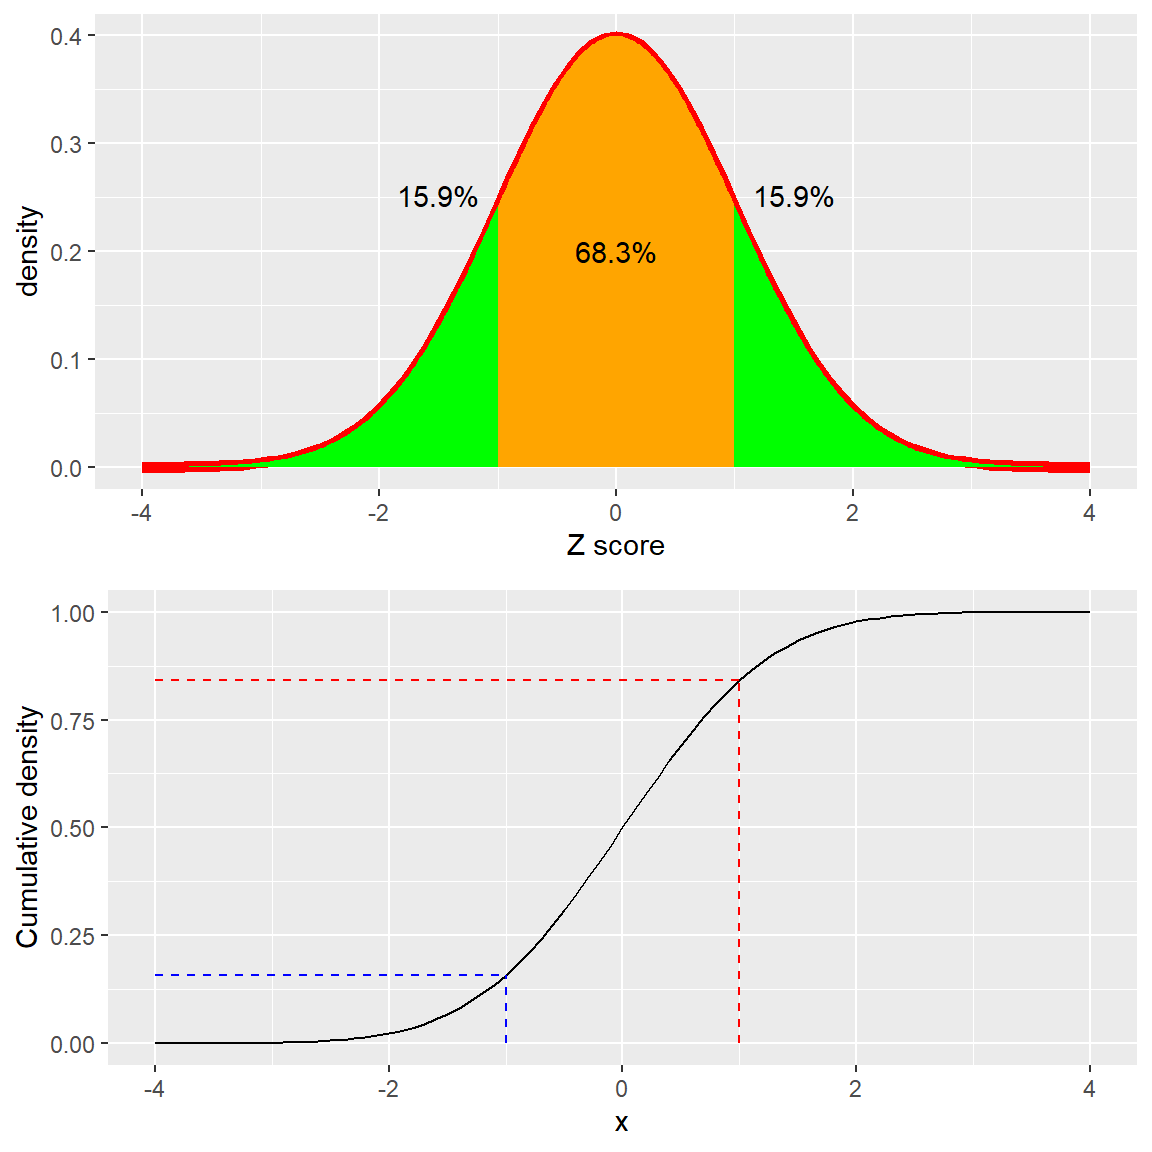
\includegraphics{StatsThinking21_files/figure-latex/zDensityCDF-1.pdf}
\caption{\label{fig:zDensityCDF}Density (top) and cumulative distribution (bottom) of a standard normal distribution, with cutoffs at one standard deviation above/below the mean.}
\end{figure}

El panel de arriba en la Figura \ref{fig:zDensityCDF} muestra que esperamos que el 16\% de los valores caigan en \(Z\ge 1\), y que la misma proporción caiga en \(Z\le -1\).

\begin{figure}
\centering
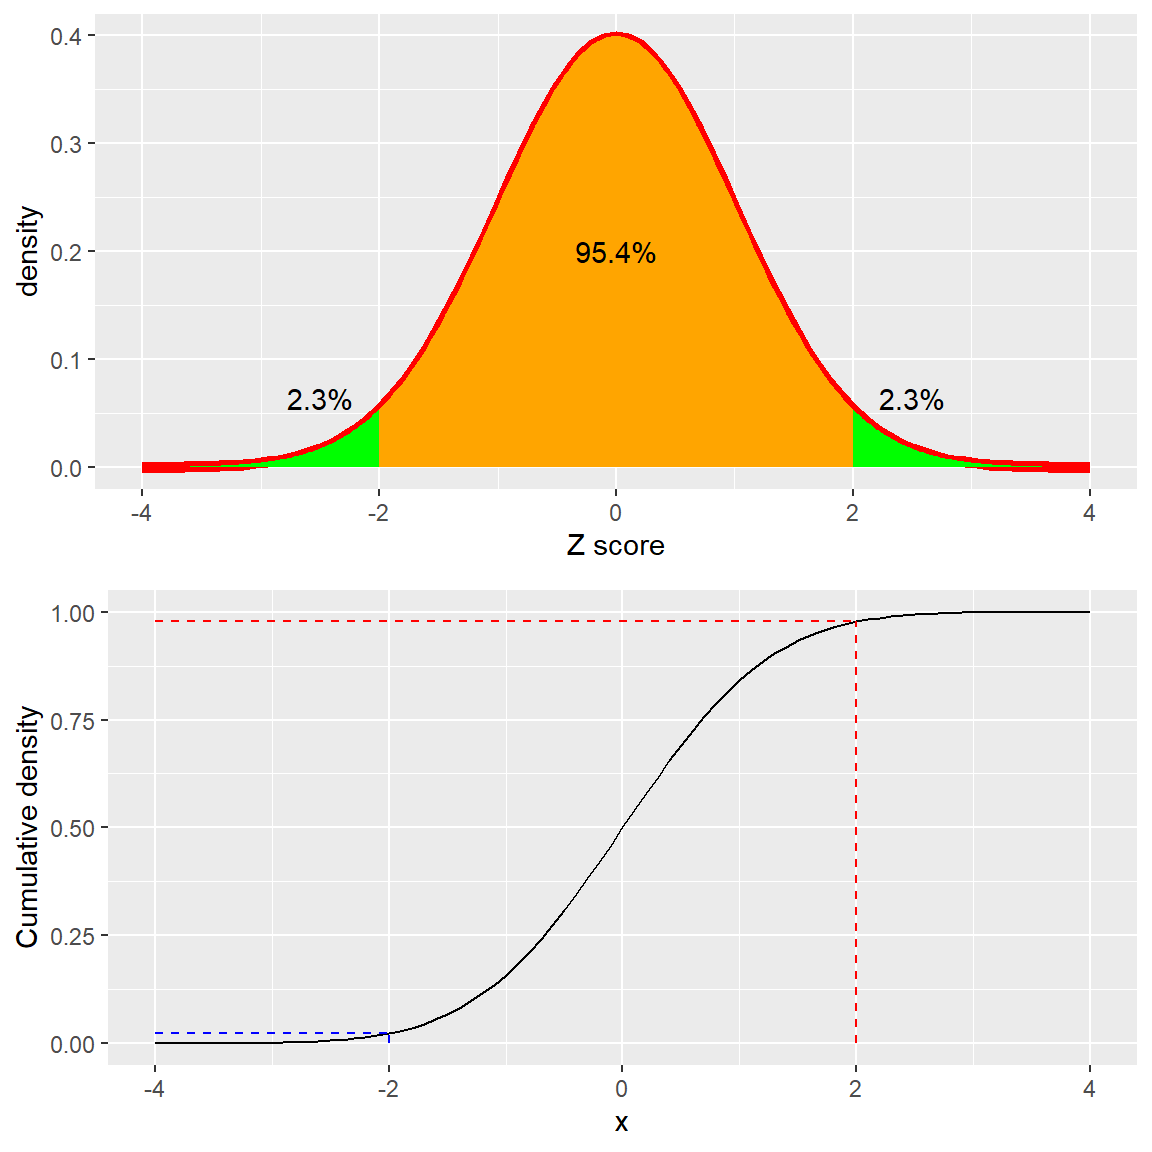
\includegraphics{StatsThinking21_files/figure-latex/zDensity2SD-1.pdf}
\caption{\label{fig:zDensity2SD}Density (top) and cumulative distribution (bottom) of a standard normal distribution, with cutoffs at two standard deviations above/below the mean}
\end{figure}

En la Figura \ref{fig:zDensity2SD} se muestra la misma gráfica para dos desviaciones estándar. Aquí podemos ver que solamente el 2.3\% de los valores caen en \(Z \le -2\) y lo mismo en \(Z \ge 2\). Por lo que, si conocemos el puntaje Z para un punto en particular de los datos podemos estimar qué tan probable o improbable sería encontrar un valor al menos tan extremo como ese valor, lo que nos permite poner los valores en un mejor contexto.

\hypertarget{puntajes-estandarizados}{%
\subsection{Puntajes Estandarizados}\label{puntajes-estandarizados}}

Digamos que en lugar de puntajes Z, queremos generar puntajes estandarizados de crimen con una media de 100 y una desviación estándar de 10. Esto es similar a la estandarización que se hace con puntajes de tests de inteligencia para generar un cociente inteligelectual (IQ, \emph{Intelligence quotient}). Podemos hacer esto al multiplicar los puntajes Z por 10 y luego sumando 100.

\begin{figure}
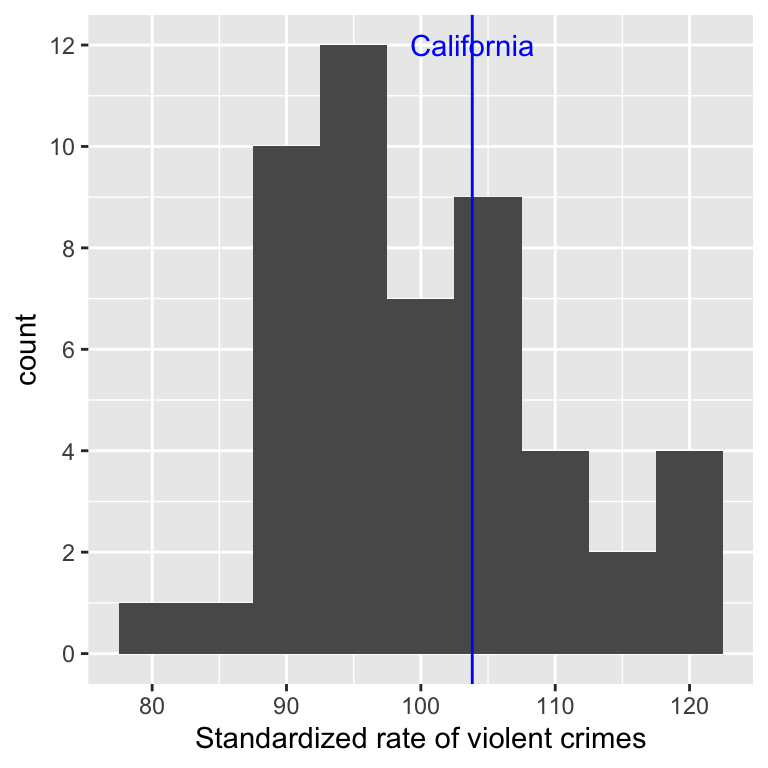
\includegraphics[height=0.5\textheight]{StatsThinking21_files/figure-latex/stdScores-1} \caption{Crime data presented as standardized scores with mean of  100 and standard deviation of 10.}\label{fig:stdScores}
\end{figure}

\hypertarget{usando-puntajes-z-para-comparar-distribuciones}{%
\subsubsection{Usando puntajes Z para comparar distribuciones}\label{usando-puntajes-z-para-comparar-distribuciones}}

Un uso útil de los puntajes Z es para comparar distribuciones de diferentes variables. Digamos que queremos comparar las distribuciones de crímenes violentos y crímenes en propiedades privadas entre estados. En el panel de la izquierda de la Figura \ref{fig:crimeTypePlot} graficamos ambos, uno contra el otro, con California representada en azul. Como puedes ver, las tasas brutas de delitos contra la propiedad son mucho más altos que las tasas brutas de crímenes violentos, por lo que no podemos solamente comparar los números directamente. Sin embargo, podemos graficar los puntajes Z para estos datos, uno contra otro (panel de la derecha de la Figura \ref{fig:crimeTypePlot}) -- Aquí de nuevo podemos ver que la distribución de los datos no cambia. Al haber puesto los datos en puntajes Z para cada variable los hace comparables, y podemos ver ahora que California está justo en el medio de la distribución en términos de crímenes violentos y crímenes de propiedad privada.

\begin{figure}
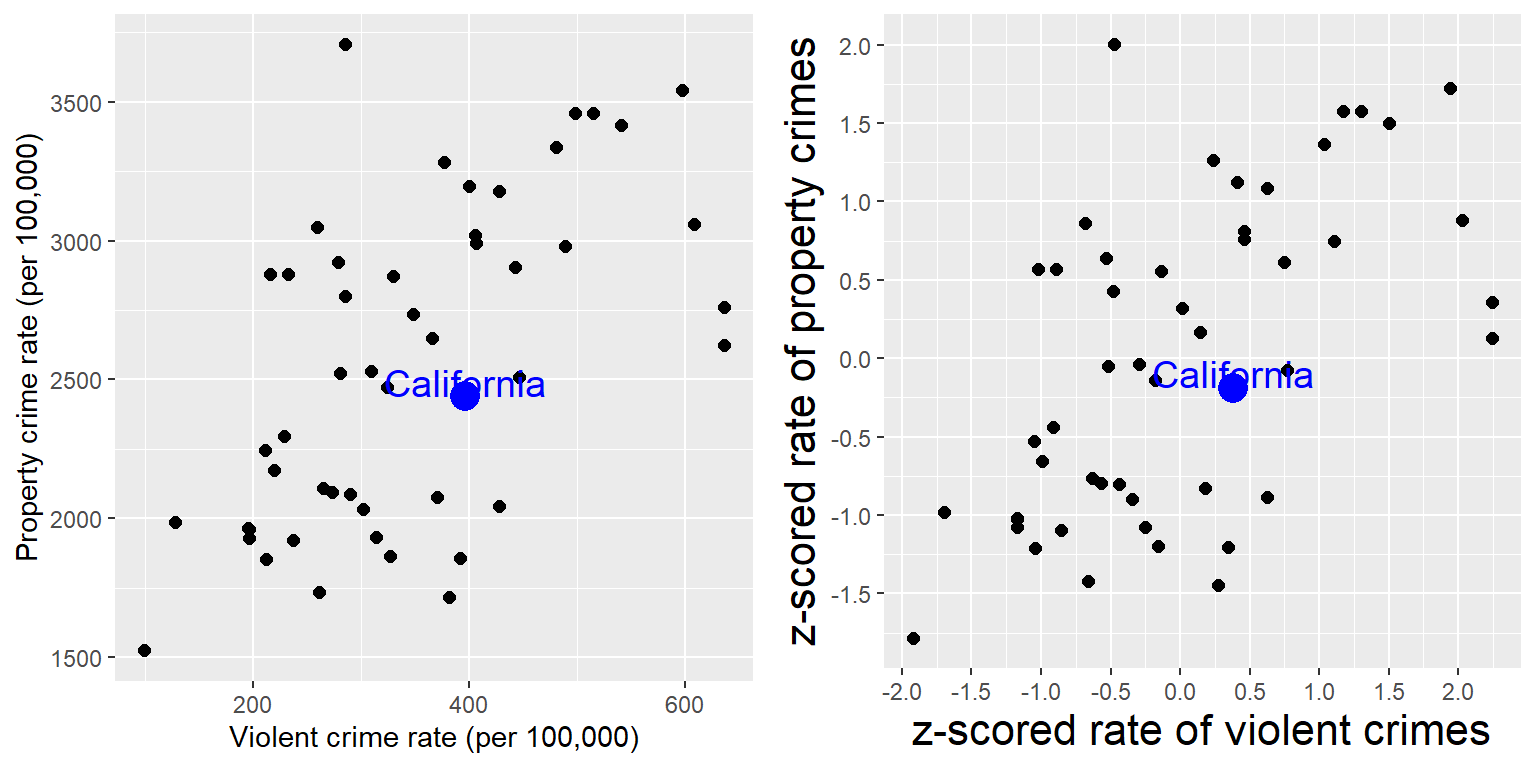
\includegraphics[height=0.5\textheight]{StatsThinking21_files/figure-latex/crimeTypePlot-1} \caption{Plot of violent vs. property crime rates (left) and Z-scored rates (right).}\label{fig:crimeTypePlot}
\end{figure}

Vamos a añadir otro factor a la gráfica: Población. En el panel izquierdo de la Figura \ref{fig:crimeTypePopPlot}, mostramos esto utilizando el tamaño del símbolo para graficar, el cual es comúnmente una forma útil de añadir información a la gráfica.

\begin{figure}
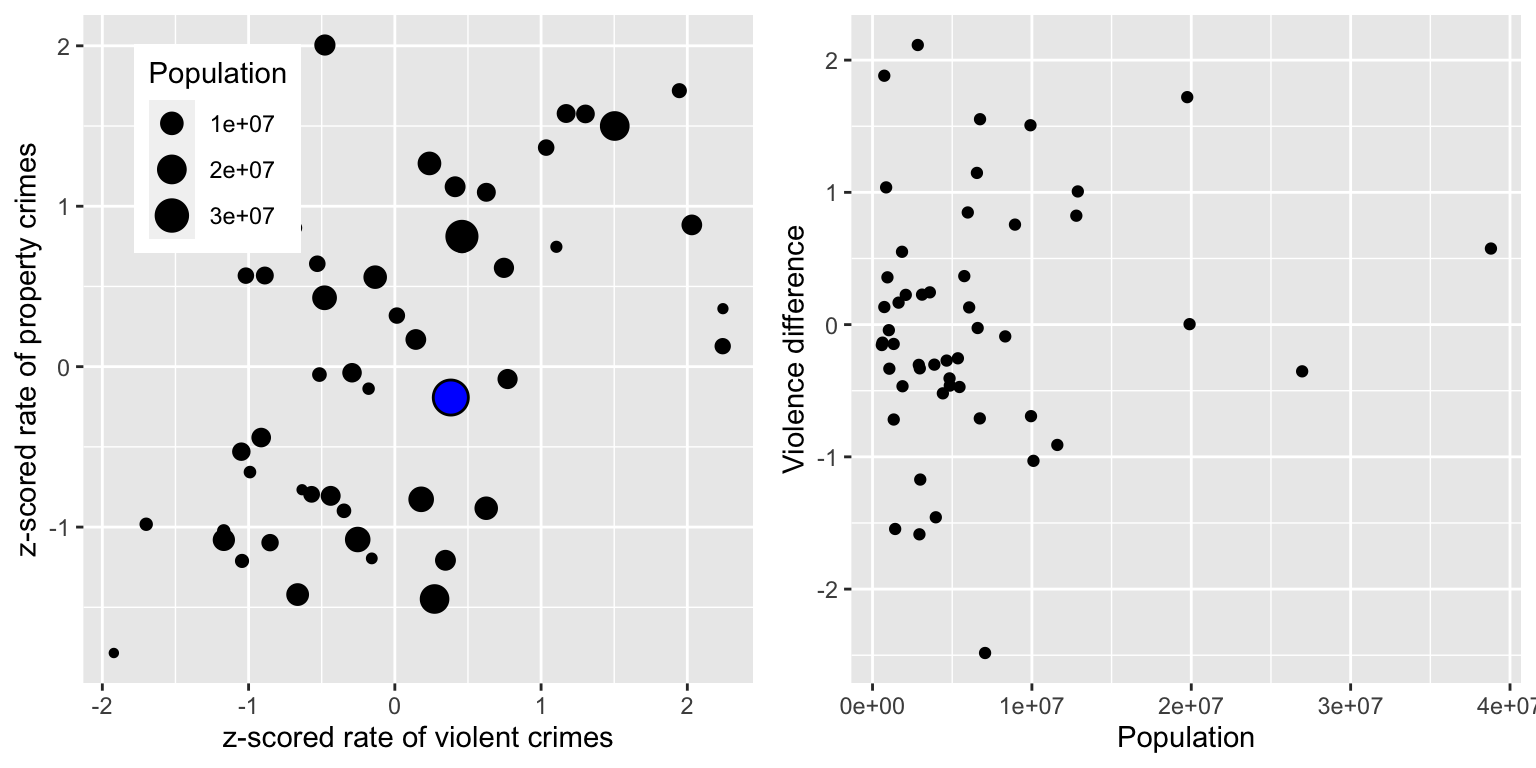
\includegraphics[height=0.5\textheight]{StatsThinking21_files/figure-latex/crimeTypePopPlot-1} \caption{Left: Plot of violent vs. property crime rates, with population size presented through the size of the plotting symbol; California is presented in blue. Right: Difference scores for violent vs. property crime, plotted against population. }\label{fig:crimeTypePopPlot}
\end{figure}

Porque los puntajes Z son directamente comparables, también podemos calcular \emph{puntuaciones diferenciales} (\emph{difference scores}), que expresen la tasa relativa de delitos violentos y no violentos (contra la propiedad) en todos los estados. Luego podemos graficar esos puntajes en comparación con la población (mira el Panel derecho de la Figura \ref{fig:crimeTypePopPlot}). Esto muestra cómo podemos usar los puntajes Z para unir diferentes variables en una escala común.

Vale la pena mencionar que los estados más pequeños parecen tener la diferencia más grande en ambas direcciones. Si bien puede ser tentador observar cada estado e intentar determinar por qué tiene una puntuación de diferencia alta o baja, esto probablemente refleja el hecho de que las estimaciones obtenidas de muestras más pequeñas necesariamente serán más variables, como discutiremos en un capítulo posterior sobre muestreo.

\hypertarget{objetivos-de-aprendizaje-4}{%
\section{Objetivos de aprendizaje}\label{objetivos-de-aprendizaje-4}}

Al leer este capítulo deberás de ser capaz de:

\begin{itemize}
\tightlist
\item
  Describir ecuaciones básicas para modelos estadísticos (outcome = model + error).
\item
  Describir diferentes mediciones de tendencia central y dispersión, cómo se calculan y cuáles son apropiadas bajo cuáles circunstancias.
\item
  Calcular puntajes Z y describir por qué son útiles.
\end{itemize}

\hypertarget{apuxe9ndice-1}{%
\section{Apéndice}\label{apuxe9ndice-1}}

\hypertarget{proof-that-the-sum-of-errors-from-the-mean-is-zero}{%
\subsection{Proof that the sum of errors from the Mean is zero''}\label{proof-that-the-sum-of-errors-from-the-mean-is-zero}}

\[
error = \sum_{i=1}^{n}(x_i - \bar{X}) = 0
\]

\[
\sum_{i=1}^{n}x_i - \sum_{i=1}^{n}\bar{X}=0
\]

\[
\sum_{i=1}^{n}x_i = \sum_{i=1}^{n}\bar{X}
\]

\[
\sum_{i=1}^{n}x_i = n\bar{X}
\]

\[
\sum_{i=1}^{n}x_i = \sum_{i=1}^{n}x_i
\]

\hypertarget{probability}{%
\chapter{Probabilidad}\label{probability}}

La teoría de probabilidad es la rama de las matemáticas que trata con el azar y la incertidumbre. Forma parte importante de los fundamentos de la estadística, porque nos provee con las herramientas matemáticas para describir eventos inciertos. El estudio de la probabilidad inició en parte debido al interés de entender los juegos de azar, como las cartas o los dados. Estos juegos proveen de ejemplos útiles de muchos conceptos estadísticos, porque cuando repetimos estos juegos la probabilidad de diferentes resultados se mantiene (mayormente) igual. Sin embargo, existen preguntas profundas sobre el significado de la probabilidad que no abordaremos aquí; ve las Lecturas Sugeridas al final del capítulo si estás interesade en aprender más acerca de este tema fascinante y su historia.

\hypertarget{quuxe9-es-la-probabilidad}{%
\section{¿Qué es la probabilidad?}\label{quuxe9-es-la-probabilidad}}

De manera informal, usualmente pensamos a la probabilidad (probability) como el número que describe la probabilidad (likelihood) de que un evento ocurra, que va de un rango desde cero (imposibilidad) a uno (certeza). A veces las probabilidades se expresarán en porcentajes, que van de un rango de cero a cien, como cuando en el pronóstico del tiempo se predice que hay un veinte por ciento de probabilidad de lluvia para hoy. En cada caso, estos números expresan qué tan probable es que suceda un evento en particular, desde la absoluta imposibilidad hasta la absoluta certeza.

Para formalizar la teoría de probabilidad, primero necesitamos definar algunos términos:

\begin{itemize}
\tightlist
\item
  Un \textbf{experimento} es cualquier actividad que produce u observa un resultado. Ejemplos son el lanzar una moneda, rodar un dado, o probar una nueva ruta al trabajo para ver si es más rápida que la vieja ruta.
\item
  El \textbf{espacio muestral} es el conjunto de posibles resultados de un experimento. Los representamos enlistándolos dentro de un par de llaves ( \{\} ). En el caso de un lanzamiento de moneda, el espacio muestral es \{cara, cruz\}. En el caso de un dado de seis lados, el espacio muestral es cada uno de los posibles números que pueden aparecer: \{1,2,3,4,5,6\}. Para el tiempo que toma llegar al trabajo, el espacio muestral son todos los posibles números reales mayores a cero (porque no se puede llegar a algún lugar en un tiempo negativo, al menos aún no se puede). No nos preocuparemos en tratar de escribir todos esos números entre las llaves.
\item
  Un \textbf{evento} es un subconjunto del espacio muestral. En principio puede ser uno o más de los posibles resultados en el espacio muestral, pero aquí nos enfocaremos principalmente en \emph{eventos elementales} que consisten en exactamente un solo posible resultado. Por ejemplo, esto podría ser el obtener cara en un solo lanzamiento de moneda, sacar un 4 en un lanzamiento de dado, o tardar 21 minutos en llegar a casa en la nueva ruta.
\end{itemize}

Ahora que tenemos estas definiciones, podemos delinear las características formales de una probabilidad, las cuales fueron primero definidas por el matemático ruso Andrei Kolmogorov. Estas son las características que \emph{debe} tener un valor si va a ser una probabilidad. Digamos que tenemos un espacio muestral definido por N eventos independientes, \({E_1, E_2, ... , E_N}\), y \(X\) es una variable aleatoria que denota cuál de los eventos ha sucedido. \(P(X=E_i)\) es la probabilidad de un evento \(i\):

\begin{itemize}
\tightlist
\item
  La probabilidad no puede ser negativa: \(P(X=E_i) \ge 0\)
\item
  La probabilidad total de todos los resultados en un espacio muestral es 1; esto es, si tomamos la probabilidad de cada \(E_i\) y las sumamos, deben dar un total de 1. Podemos expresar esto usando el símbolo de sumatoria \(\sum\):
  \[
  \sum_{i=1}^N{P(X=E_i)} = P(X=E_1) + P(X=E_2) + ... + P(X=E_N) = 1
  \]
  Esto se interpreta como ``Toma todos los eventos elementales N, que hemos etiquetado desde 1 hasta N, y suma sus probabilidades. Estas deben sumar 1.''
\item
  La probabilidad de cualquier evento individual no puede ser mayor a uno: \(P(X=E_i)\le 1\). Esto es sugerido por el punto anterior; como deben de sumar uno, y no pueden ser números negativos, entonces cualquier probabilidad en particular debe ser menor o igual a uno.
\end{itemize}

\hypertarget{cuxf3mo-determinamos-probabilidades}{%
\section{¿Cómo determinamos probabilidades?}\label{cuxf3mo-determinamos-probabilidades}}

Ahora que sabemos lo que es la probabilidad, ¿cómo hacemos para realmente averiguar cuál es la probabilidad de que suceda algún evento en particular?

\hypertarget{creencia-personal}{%
\subsection{Creencia personal}\label{creencia-personal}}

Digamos que te pregunto cuál hubiera sido la probabilidad de que los Beatles hubieran sido igualmente exitosos si no hubieran reemplazado al baterista original Pete Best por Ringo Starr en 1962. Definiremos ``éxito'' en términos de la cantidad de hits número uno en el Billboard Hot 100 (al que nos referiremos como \(N_{hits}\)); los Beatles tuvieron 20 de esos hits número uno, por lo que el espacio muestral es \{ \(N_{hits} < 20\),\(N_{hits} \ge 20\) \}. No podemos realmente hacer el experimento para averiguar el resultado. Sin embargo, la mayoría de las personas con conocimiento de los Beatles estarían dispuestos a por lo menos a tratar de adivinar la probabilidad de este evento. En muchos casos el conocimiento personal y/u opinión es la única guía que tenemos para determinar la probabilidad de un evento, pero esto no es muy satisfactorio científicamente.

\hypertarget{empirical-frequency}{%
\subsection{Frecuencia empírica}\label{empirical-frequency}}

Otra manera de determinar la probabilidad de un evento es el hacer un experimento muchas veces y contar cuántas veces sucedió cada evento. Podemos calcular la probabilidad de cada resultado a partir de la frecuencia relativa de los diferentes resultados. Por ejemplo, digamos que estás interesado en saber la probabilidad de lluvia en San Francisco. Primero debemos definir nuestro experimento --- digamos que miraremos los datos del \emph{National Weather Service} para cada día en 2017 y determinaremos si hubo lluvia en la estación del clima del centro de San Francisco.

\begin{tabular}{r|r|r}
\hline
Number of rainy days & Number of days measured & P(rain)\\
\hline
73 & 365 & 0.2\\
\hline
\end{tabular}

De acuerdo con estos datos, en 2017 hubo 73 días lluviosos. Para calcular la probabilidad de lluvia en San Francisco, simplemente dividimos el número de días lluviosos entre el número de días totales (365), dando una P(lluvia en SF en 2017) = 0.2

¿Cómo sabemos que la probabilidad empírica nos dará el número correcto? La respuesta a esta pregunta viene de la \emph{ley de números grandes}, que muestra que la probabilidad empírica se aproximará a la verdadera probabilidad conforme el tamaño de la muestra se incrementa. Podemos ver esto simulando un gran número de lanzamientos de moneda, y observando nuestra estimación de la probabilidad de que caiga cara después de cada lanzamiento. Pasaremos más tiempo discutiendo simulaciones en un capítulo posterior; por ahora, sólo asumamos que tenemos una manera computacional de generar un resultado aleatorio para cada lanzamiento de moneda.

El panel izquierdo de la Figura \ref{fig:ElectionResults} muestra que conforme el número de muestras (i.e., ensayos de lanzamiento de moneda) incrementa, la probabilidad estimada de obtener cara converge en el valor verdadero de 0.5. Sin embargo, nota que las estimaciones pueden estar bastante lejos del valor verdadero cuando los tamaños de muestra son pequeños. Un ejemplo del mundo real sobre esto se puede ver en la elección especial de 2017 para el Senado de EUA en Alabama, que enfrentó al Republicano Roy Moore contra el Demócrata Doug Jones. El panel derecho de la Figura \ref{fig:ElectionResults} muestra la cantidad relativa de votos reportados para cada uno de los candidatos en el curso de la tarde del día de la elección, conforme un número creciente de boletas eran contadas. Temprano en la tarde el conteo de votos era especialmente volátil, balanceándose desde una ventaja inicial grande para Jones hasta un periodo largo donde Moore tenía la ventaja, hasta que finalmente Jones tomó la delantera ganando la contienda.

\begin{figure}
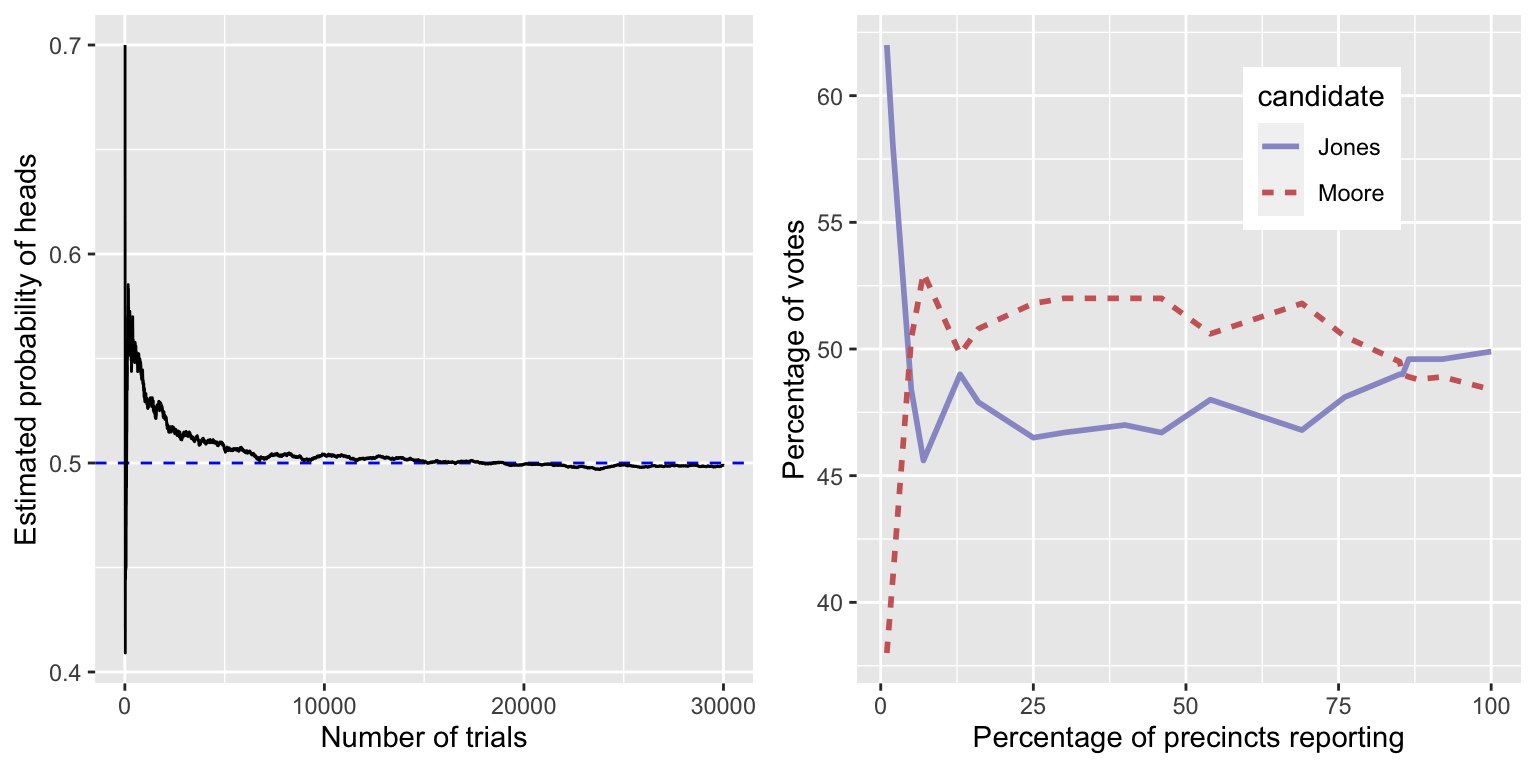
\includegraphics[height=0.5\textheight]{StatsThinking21_files/figure-latex/ElectionResults-1} \caption{Izquierda: Una demostración de la ley de los números grandes. Una moneda fue lanzada 30,000 veces, y después de cada lanzamiento la probabilidad de obtener cara era calculada basada en el número de caras y cruces observadas hasta ese punto. Toma un aproximado de 15,000 lanzamientos para que la probabilidad se quede establecida en la probabilidad verdadera de 0.5. Derecha: Proporción relativa de votos el 12 de diciembre de 2017 durante la elección especial para el asiento de Alabama en el Senado de EUA, como una función del porcentaje de casillas electorales reportadas. Estos datos fueron transcritos de https://www.ajc.com/news/national/alabama-senate-race-live-updates-roy-moore-doug-jones/KPRfkdaweoiXICW3FHjXqI/ }\label{fig:ElectionResults}
\end{figure}

Estos dos ejemplos muestran que mientras las muestras grandes últimamente convergen en la probabilidad verdadera, los resultados de muestras pequeñas pueden estar muy equivocados. Desafortunadamente, muchas personas olvidan esto y sobreinterpretan resultados de muestras pequeñas. Esto ha sido referido como la \emph{ley de números pequeños} por los psicólogos Danny Kahneman y Amos Tversky, quienes mostraron que la gente (incluso investigadores entrenados) frecuentemente se comportan como si la ley de los números grandes aplicara también en las muestras pequeñas, dando demasiada credibilidad a resultados de bases de datos pequeñas. A lo largo del curso veremos ejemplos de qué tan inestables pueden ser los resultados estadísticos cuando son generados en base a muestras pequeñas.

\hypertarget{probabilidad-cluxe1sica}{%
\subsection{Probabilidad clásica}\label{probabilidad-cluxe1sica}}

Es poco probable que cualquiera de nosotros haya lanzado una moneda decenas de miles de veces, pero sin importar eso estamos dispuestos a creer que la probabilidad de lanzar una moneda y que caiga cara es 0.5. Esto refleja el uso de otra aproximación más al cálculo de probabilidades, al cual nos referimos como \emph{probabilidad clásica}. En esta aproximación, calculamos la probabilidad directamente desde nuestro conocimiento de la situación.

La probabilidad clásica surgió del estudio de juegos de azar como los dados y las cartas. Un ejemplo famoso surgió del problema que se encontró un jugador francés que se conocía por el nombre de Chevalier de Méré. de Méré jugaba dos diferentes juegos de dados: En el primero él apostaba en la probabilidad de obtener por lo menos un seis en cuatro lanzamientos de un dado de seis lados, mientras que en el segundo juego apostaba en la probabilidad de obtener por lo menos un doble seis en 24 lanzamientos de dos dados. Él esperaba ganar dinero en ambos juegos, pero encontró que mientras que en promedio él ganaba dinero en el primer juego, realmente terminaba perdiendo dinero en promedio cuando jugaba el segundo juego muchas veces. Para entender esto buscó a su amigo, el matemático Blaise Pascal, quien es reconocido como uno de los fundadores de la teoría de probabilidad.

¿Cómo podemos entender esta pregunta usando teoría de probabilidad? En probabilidad clásica, comenzamos con una suposición de que todos los eventos elementales en el espacio muestral son igualmente probables; esto es, cuando lanzas un dado, cada uno de los posibles resultados (\{1,2,3,4,5,6\}) es igualmente probable que ocurra. (¡No se permiten dados cargados (o manipulados)! Considerando esto, podemos calcular la probabilidad de cualquier resultado individual como un uno dividido entre el número de resultados posibles:

\[
P(resultados_i) = \frac{1}{\text{número de resultados posibles}}
\]

Para el dado de seis lados, la probabilidad de cada resultados individual es 1/6.

Esto está bien, pero de Méré estaba interesado en eventos más complejos, como lo que sucede en múltiples lanzamientos de dados. ¿Cómo calculamos la probabilidad de un evento complejo (el cual es la \emph{unión} de eventos simples), como obtener un seis en el primer \emph{o} el segundo lanzamiento?

La unión de eventos la representamos matemáticamente usando el símbolo \(\cup\): por ejemplo, si la probabilidad de obtener un seis en el primer lanzamiento es referido como \(P(Roll6_{throw1})\) y la probabilidad de obtener un seis en el segundo lanzamiento es \(P(Roll6_{throw2})\), entonces la unión es referida como \(P(Roll6_{throw1} \cup Roll6_{throw2})\).

de Méré pensó (incorrectamente, como veremos más abajo) que simplemente podía sumar las probabilidades de cada evento individual para calcular la probabilidad del evento combinado, significando que la probabilidad de obtener un seis en el primer o segundo lanzamiento se calcularía de la siguiente manera:

\[
P(Roll6_{throw1}) = 1/6
\]
\[
P(Roll6_{throw2}) = 1/6
\]

\[
de Méré's \ error:
\]
\[
P(Roll6_{throw1} \cup Roll6_{throw2}) = P(Roll6_{throw1}) + P(Roll6_{throw2}) = 1/6 + 1/6 = 1/3
\]

de Méré creyó, basado en esta suposición incorrecta, que la probabilidad de obtener al menos un seis en cuatro lanzamientos era la suma de las probabilidades de cada lanzamiento individual: \(4*\frac{1}{6}=\frac{2}{3}\). De manera similar, creyó que dado que la probabilidad de un doble seis al lanzar un dado es 1/36, entonces la probabilidad de obtener al menos un doble seis en 24 lanzamientos de dos dados sería \(24*\frac{1}{36}=\frac{2}{3}\). Sin embargo, mientras consistentemente él ganaba dinero en la primera apuesta, perdía dinero con la segunda. ¿Por qué pasaba esto?

Para entender el error de de Méré, necesitamos presentar algunas de las reglas de la teoría de probabilidad. La primera es la \emph{regla de substracción/resta}, que dice que la probabilidad de que algún evento A \emph{no} suceda es uno menos la probabilidad de que el evento suceda:

\[
P(\neg A) = 1 - P(A)
\]

donde \(\neg A\) significa ``no A''. Esta regla se deriva directamente de los axiomas que discutimos arriba; porque A y \(\neg A\) son los únicos posibles resultados, entonces su probabilidad total debe sumar 1. Por ejemplo, si la probabilidad de obtener un uno en un solo lanzamiento es \(\frac{1}{6}\), entonces la probabilidad de obtener cualquier otro número que no fuera uno es \(\frac{5}{6}\).

Una segunda regla nos dice cómo calcular la probabilidad de un evento conjunto -- esto es, la probabilidad de que ambos eventos ocurran. Nos referimos a esto como una \emph{intersección}, que es representada por el símbolo \(\cap\); por lo tanto, \(P(A \cap B)\) significa la probabilidad de que ambos A y B sucedan.

Esta versión de la regla nos dice cómo calcular esta cantidad en el caso especial cuando dos eventos son independientes uno de otro; aprenderemos después exactamente qué significa el concepto de \emph{independencia}, pero por ahora podemos dar por sentado que los dos lanzamientos de dados son eventos independientes. Calculamos la probabilidad de la intersección de dos eventos independientes simplemente multiplicando las probabilidades de los eventos individuales:

\[
P(A \cap B) = P(A) * P(B)\ \text{si y sólo si A y B con independientes}
\]
Por lo tanto, la probabilidad de obtener un seis en ambos lanzamientos de dados es \(\frac{1}{6}*\frac{1}{6}=\frac{1}{36}\).

La tercera regla nos dice cómo sumar las probabilidades - y es aquí donde vemos el origen del error de de Méré. La \emph{regla de la suma} nos dice que para obtener la probabilidad de que cualquiera de dos eventos ocurran, debemos sumar las probabilidades individuales, pero luego debemos restar la probabilidad de que ocurran ambos eventos juntos:

\[
P(A \cup B) = P(A) + P(B) - P(A \cap B)
\]
En un sentido, esto evita que contemos esos eventos conjuntos dos veces, eso es lo que distingue a esta regla del cálculo que de Méré había hecho incorrectamente. Digamos que queremos encontrar la probabilidad de obtener 1 en cualquiera de dos lanzamientos. De acuerdo a nuestras reglas:

\[
P(Roll1_{throw1} \cup Roll1_{throw2}) 
\]
\[
= P(Roll1_{throw1}) + P(Roll1_{throw2}) - P(Roll1_{throw1} \cap Roll1_{throw2}) 
\]
\[
= \frac{1}{6} + \frac{1}{6} - \frac{1}{36} = \frac{11}{36}
\]

\begin{figure}
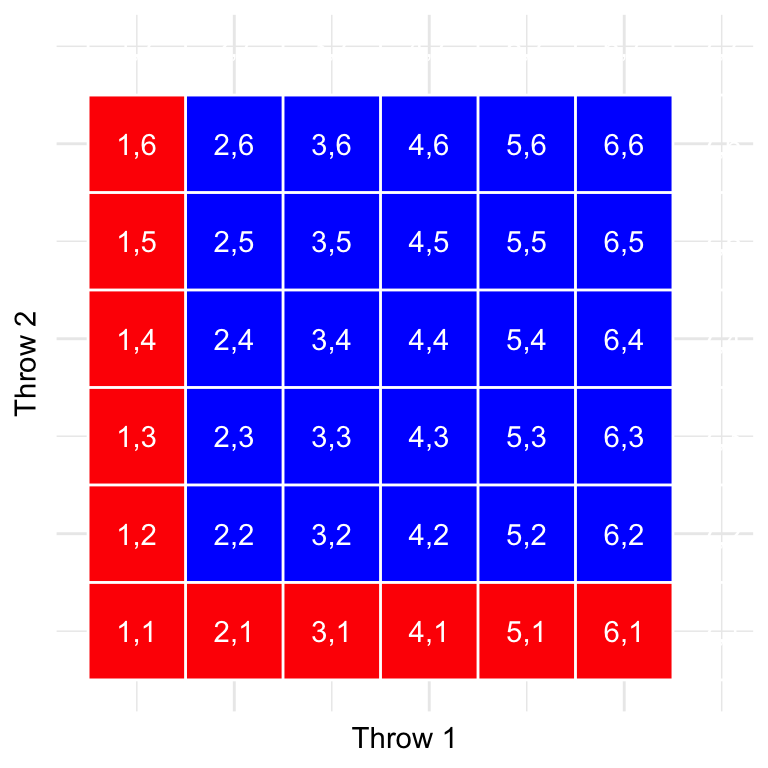
\includegraphics[height=0.5\textheight]{StatsThinking21_files/figure-latex/ThrowMatrix-1} \caption{Cada celda de esta matriz representa un resultado de dos lanzamientos de un solo dado, donde las columnas representan el primer lanzamiento y las filas representan el segundo lanzamiento. Las celdas en rojo representan celdas con un uno ya sea en el primer o en el segundo lanzamiento; el resto se muestran en azul. }\label{fig:ThrowMatrix}
\end{figure}

Usemos una representación gráfica para obtener una diferente vista de esta regla. La Figura \ref{fig:ThrowMatrix} muestra una matriz representando todas las posibles combinaciones de resultados de dos lanzamientos de dados, y subraya las celdas que involucran un uno ya sea en el primer o en el segundo lanzamiento. Si cuentas las celdas en rojo verás que hay 11 celdas con ese resultado. Esto muestra por qué la regla de la suma da una respuesta diferente a la de de Méré; si simplemente sumáramos las probabilidades de los dos lanzamientos como él lo hizo, entonces terminaríamos contando la celda de (1,1) en ambos, cuando solamente debería contar una sola vez.

\hypertarget{resolviendo-el-problema-de-de-muxe9ruxe9}{%
\subsection{Resolviendo el problema de de Méré}\label{resolviendo-el-problema-de-de-muxe9ruxe9}}

Blaise Pascal usó la reglas de la probabilidad para idear una solución al problema de de Méré. Primero, se dio cuenta que calcular la probabilidad de al menos un evento de una combinación era complicado, mientras que calcular la probabilidad de que algo no ocurra a lo largo de varios eventos es relativamente fácil -- es sólo el producto de las probabilidades de los eventos individuales. Por lo tanto, en lugar de calcular la probabilidad de al menos un seis en cuatro lanzamientos, calculó la probabilidad de ningún seis a lo largo de todos los lanzamientos:

\[
P(\text{ningún seis en cuatro lanzamientos})
\]
\[
= \frac{5}{6}*\frac{5}{6}*\frac{5}{6}*\frac{5}{6}=\bigg(\frac{5}{6}\bigg)^4=0.482
\]

Pascal entonces usó el hecho de que la probabilidad de ningún seis en cuatro lanzamientos es el complemento de al menos un seis en cuatro lanzamientos (por lo que deben sumar uno), y usó la regla de la resta para calcular la probabilidad de interés:

\[
P(\text{al menos un seis en cuatro lanzamientos}) = 1 - \bigg(\frac{5}{6}\bigg)^4=0.517
\]

La apuesta de de Méré de que obtendría al menos un seis en cuatro lanzamientos tiene una probabilidad mayor a 0.5, lo que explica por qué de Méré ganaba dinero en esta apuesta en promedio.

¿Pero qué pasaba con la segunda apuesta de de Méré? Pascal usó el mismo truco:

\[
P(\text{no doble seis en 24 lanzamientos}) = \bigg(\frac{35}{36}\bigg)^{24}=0.509
\]
\[
P(\text{al menos un doble seis en 24 lanzamientos}) = 1 - \bigg(\frac{35}{36}\bigg)^{24}=0.491
\]

La probabilidad de este resultado era ligeramente menor a 0.5, mostrando por qué de Méré perdía dinero con esta apuesta en promedio.

\hypertarget{distribuciones-de-probabilidad}{%
\section{Distribuciones de probabilidad}\label{distribuciones-de-probabilidad}}

Una \emph{distribución de probabilidad} describe la probabilidad de todos los posibles resultados en un experimento. Por ejemplo, el 20 de enero de 2018, el jugador de basketball Steph Curry anotó sólo 2 de 4 lanzamientos libres en un juego contra los Houston Rockets. Sabemos que la probabilidad general de Curry de anotar en lanzamientos libres a lo largo de toda la temporada fue de 0.91, por lo que parece bastante poco probable que sólo hubiera anotado 50\% de sus lanzamientos libres en un juego, ¿pero exactamente qué tan poco probable es? Podemos determinar esto usando una distribución de probabilidad teórica; durante este curso nos encontraremos con una variedad de estas distribuciones de probabilidad, cada una es apropiada para describir diferentes tipos de datos. En este caso, usaremos la distribución \emph{binomial}, que provee una manera de calcular la probabilidad de un número de éxitos en un número de ensayos en donde se puede tener sólo un éxito o un fallo y nada intermedio (conocidos como ``ensayos de Bernoulli'') dada una probabilidad conocida de éxito en cada ensayo. Esta distribución es definida como:

\[
P(k; n,p) = P(X=k) = \binom{n}{k} p^k(1-p)^{n-k}
\]

Esto se refiere a la probabilidad de k éxitos en n ensayos cuando la probabilidad de éxito es p.~Tal vez no estés familiarizado con \(\binom{n}{k}\), a la que nos referimos como el \emph{coeficiente binomial}. El coeficiente binomial también es conocido como ``n-choose-k'' porque describe el número de maneras diferentes en las que uno puede elegir k elementos de un total de elementos n.~El coeficiente binomial es calculado como:

\[
\binom{n}{k} = \frac{n!}{k!(n-k)!}
\]
donde el signo de exclamación (!) se refiere al \emph{factorial} de un número:

\[
n! = \prod_{i=1}^n i = n*(n-1)*...*2*1 
\]

En el ejemplo de los lanzamientos libres de Steph Curry:

\[
P(2;4,0.91) = \binom{4}{2} 0.91^2(1-0.91)^{4-2} = 0.040
\]

Esto demuestra que dado el porcentaje de anotaciones en lanzamientos libres de Curry en la temporada, era bastante improbable que anotara sólo 2 de 4 tiros libres. Esto sólo muestra que en el mundo real efectivamente suceden cosas improbables.

\hypertarget{distribuciones-de-probabilidad-acumuladas}{%
\subsection{Distribuciones de probabilidad acumuladas}\label{distribuciones-de-probabilidad-acumuladas}}

Frecuentemente queremos conocer no sólo qué tan probable es un valor en específico, sino saber qué tan probable es encontrar un valor que es igualmente extremo o más extremo que cierto valor en particular; esto se volverá muy importante cuando discutamos las pruebas de hipótesis en un capítulo posterior. Para contestar esta pregunta, podemos usar la distribución de probabilidad \emph{acumulada}; mientras que la distribución de probabilidad estándar nos dice la probabilidad de un valor en específico, la distribución acumulada nos dice la probabilidad de un valor igual de grande o mayor (o igual de pequeño o menor) que un valor específico.

En el ejemplo del tiro libre, tal vez quisiéramos saber: ¿Cuál es la probabilidad de que Steph Curry anotara 2 \emph{o menos} de un total de cuatro tiros libres, dado que su probabilidad general de anotar un tiro libre es de 0.91? Para determinar esto, podríamos simplemente usar la ecuación de probabilidad binomial y alimentarla con todos los valores posibles de k y sumarlos todos juntos:

\[
P(k\le2)= P(k=2) + P(k=1) + P(k=0) = 6e^{-5} + .002 + .040 = .043  
\]

En muchos casos el número de resultados posibles podría ser demasiado grande para poder calcular la probabilidad acumulada con este método de enumerar todos los valores posibles; afortunadamente, puede ser calculado directamente para cualquier distribución de probabilidad teórica. La Tabla \ref{tab:CurryCumulativeProb} muestra la probabilidad acumulada de cada número posible de tiros libres exitosos del ejemplo de arriba:

\begin{table}

\caption{\label{tab:CurryCumulativeProb}Distribución de probabilidad acumulada para el número de tiros libres exitosos en los 4 intentos de Steph Curry.}
\centering
\begin{tabular}[t]{r|r}
\hline
numSuccesses & CumulativeProbability\\
\hline
0 & 0.000\\
\hline
1 & 0.003\\
\hline
2 & 0.043\\
\hline
3 & 0.314\\
\hline
4 & 1.000\\
\hline
\end{tabular}
\end{table}

De la tabla podemos ver que la probabilidad de que Curry anotara 2 o menos tiros libres de un total de 4 intentos es 0.043.

\hypertarget{conditional-probability}{%
\section{Probabilidad condicional}\label{conditional-probability}}

Hasta ahora nos hemos limitado a probabilidades simples - esto es, la probabilidad de un solo evento o combinación de eventos. Sin embargo, frecuentemente deseamos determinar la probabilidad de algunos eventos dependiendo de que otro evento haya ocurrido, lo cual se conoce como \emph{probabilidad condicional}.

Tomemos como ejemplo la elección Presidencial de EUA en 2016. Existen dos probabilidades simples que podríamos usar para describir al electorado. Primero, conocemos la probabilidad de que un votante en EUA esté afiliado al Partido Republicano: \(p(Republican) = 0.44\). También conocemos la probabilidad de que un votante dé su voto en favor de Donald Trump: \(p(Trump voter)=0.46\). Sin embargo, digamos que queremos saber lo siguiente: ¿Cuál es la probabilidad de que una persona vote por Donald Trump, \emph{dado que esa persona sea Republicana}?

Para calcular la probabilidad condicional de A dado B (que escribimos como \(P(A|B)\), ``probabilidad de A, dado B''), necesitamos conocer la \emph{probabilidad conjunta} (esto es, la probabilidad de que ambos A y B ocurran) así como la probabilidad general de B:

\[
P(A|B) = \frac{P(A \cap B)}{P(B)}
\]

Esto es, queremos saber la probabilidad de que ambas cosas sean ciertas, dado que aquella sobre la que está condicionada sea cierta.

\begin{figure}
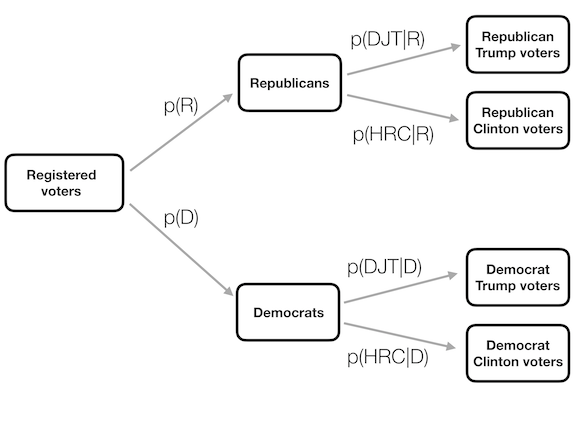
\includegraphics[height=0.5\textheight]{images/conditional_probability} \caption{Representación gráfica de la probabilidad condicional, mostrando cómo la probabilidad condicional limita nuestro análisis a un subconjunto de los datos.}\label{fig:conditionalProbability}
\end{figure}

Puede ser útil pensar en esto gráficamente. La Figura \ref{fig:conditionalProbability} muestra un diagrama de flujo que representa cómo el total de la población de votantes se divide en Republicanos y Demócratas, y cómo la probabilidad condicional (condicinada sobre el partido) divide aún a los miembros de cada partido de acuerdo a su voto.

\hypertarget{calcular-probabilidades-condicionales-a-partir-de-los-datos}{%
\section{Calcular probabilidades condicionales a partir de los datos}\label{calcular-probabilidades-condicionales-a-partir-de-los-datos}}

También podemos calcular probabilidades condicionales desde los datos. Digamos que estamos interesados en la siguiente pregunta: ¿Cuál es la probabilidad de que alguien tenga diabetes, dado que no sea una persona físicamente activa? -- esto es, \(P(diabetes|inactive)\). La base de datos NHANES incluye dos variables que abordan las dos partes de esta pregunta. La primera (\texttt{Diabetes}) pregunta si una persona ha sido enterada de que tenga diabetes, y la segunda (\texttt{PhysActive}) registra si una persona se involucra en deportes, fitness, o actividades recreativas que sean de al menos intensidad moderada. Primero calculemos las probabilidades simples.

\begin{table}

\caption{\label{tab:DiabetesPhysActiveSummary}Resumen de datos para diabetes y actividad física}
\centering
\begin{tabular}[t]{l|r|r|r|r}
\hline
Answer & N\_diabetes & P\_diabetes & N\_PhysActive & P\_PhysActive\\
\hline
No & 4893 & 0.9 & 2472 & 0.45\\
\hline
Yes & 550 & 0.1 & 2971 & 0.55\\
\hline
\end{tabular}
\end{table}

La Tabla \ref{tab:DiabetesPhysActiveSummary} muestra la probabilidad de que alguien en la base de datos NHANES tenga diabetes es .1, y la probabilidad de que alguien sean inactivo es .45.

\begin{table}

\caption{\label{tab:DiabetesPhysActiveSummaryJoint}Joint probabilities for Diabetes and PhysActive variables.}
\centering
\begin{tabular}[t]{l|l|r|r}
\hline
Diabetes & PhysActive & n & prob\\
\hline
No & No & 2123 & 0.39\\
\hline
No & Yes & 2770 & 0.51\\
\hline
Yes & No & 349 & 0.06\\
\hline
Yes & Yes & 201 & 0.04\\
\hline
\end{tabular}
\end{table}

Para calcular \(P(diabetes|inactive)\) necesitaríamos también conocer la probabilidad conjunta de ser diabético \emph{y} ser inactivo, además de las probabilidades simples de cada uno.

Basados en estas probabilidades conjuntas, podemos calcular \(P(diabetes|inactive)\). Una manera de hacer esto en un programa de computadora es primero determinar si la variable PhysActive era igual a ``No'' en cada individuo, y luego obtener la media de esos valores. Debido a que los valores TRUE/FALSE son tratados como 1/0 respectivamente por la mayoría de los lenguajes de programación (incluidos R y Python), esto nos permite identificar fácilmente la probabilidad de un evento simple obteniendo simplemente la media de una variable lógica que representa si el valor era verdadero. Entonces usamos ese valor para calcular la probabilidad condicional, donde podemos encontrar la probabilidad de que alguien tenga diabetes dado que sea una persona físicamente inactiva es 0.141.

\hypertarget{independencia}{%
\section{Independencia}\label{independencia}}

El término ``independiente'' tiene un significado muy específico en estadística, que es un poco diferente del uso común del término. Independencia estadística entre dos variables significa que el conocer el valor de una variable no dice nada sobre el valor de la otra. Esto puede ser expresado como:

\[
P(A|B) = P(A)
\]

Esto es, la probabilidad de A dado algún valor de B es la misma que la probabilidad general de A. Mirándolo de esta manera, podemos ver que muchos casos de lo que llamaríamos ``independencia'' en el mundo real no son realmente estadísticamente independientes. Por ejemplo, actualmente hay un movimiento de un pequeño grupo de ciudadanos de California que quiere declarar un nuevo estado independiente llamado Jefferson, que comprendería a un número de condados del norte de California y Oregon. Si esto pasara, entonces la probabilidad de que un residente actual de California ahora viviera en el estado de Jefferson sería \(P(\text{Jeffersonian})=0.014\), mientras que la probabilidad de que se mantuviera siendo un residente de California sería \(P(\text{Californian})=0.986\). Los nuevos estados serían políticamente independientes, pero \emph{no} serían estadísticamente independientes, porque ¡\(P(\text{Californian|Jeffersonian}) = 0\)! Esto es, mientras que independencia en el lenguaje común frecuentemente se refiere a conjuntos que son excluyentes, independencia estadística se refiere al caso donde no se puede predecir nada sobre una variable del valor de otra variable. Por ejemplo, conocer el color de cabello de una persona es improbable que te diga algo sobre si la persona prefiere nieve de chocolate o fresa.

Revisemos otro ejemplo, usando la base de datos NHANES: ¿La salud mental y la salud física son independientes la una de la otra? NHANES incluye dos preguntas relevantes: \emph{PhysActive}, que pregunta si un individuo es físicamente activo, y \emph{DaysMentHlthBad}, que pregunta cuántos días en los últimos 30 días la persona ha experimentado malos días de salud mental. Consideremos a cualquiera que haya tenido más de 7 días de mala salud mental en el último mes como parte de un grupo con mala salud mental. Basados en esto, podemos definir una nueva variable llamada \emph{badMentalHealth} como una variable lógica que nos diga si la persona ha tenido más de 7 días con mala salud mental o no. Usando esta nueva variable, podemos entonces determinar si mala salud mental y actividad física son independientes preguntándonos si la probabilidad simple de mala salud mental es diferente de la probabilidad condicional de mala salud mental dado que la persona sea físicamente activa.

\begin{tabular}{l|r}
\hline
PhysActive & badMentalHealth\\
\hline
No & 0.20\\
\hline
Yes & 0.13\\
\hline
\end{tabular}

La probabilidad general de mala salud mental \(P(\text{bad mental health})\) es 0.16 mientras que la probabilidad condicional \(P(\text{bad mental health|physically active})\) es 0.13. Por lo tanto, parece ser que la probabilidad condicional es un poco menor que la probabilidad general, sugiriendo que no son independientes, aunque no podemos saber con certeza sólo observando estos números, porque estos números podrían ser diferentes debido a variabilidad aleatoria en nuestra muestra. Más tarde en este curso encontraremos herramientas que nos permitirán probar de manera más directa si estas variables son independientes.

\hypertarget{bayestheorem}{%
\section{Invertir una probabilidad condicional: regla de Bayes}\label{bayestheorem}}

En muchos casos, conocemos \(P(A|B)\) pero lo que realmente queremos conocer es \(P(B|A)\). Esto comúnmente ocurre en tamizajes (screenings) médicos, donde conocemos \(P(\text{resultado positivo en un test| enfermedad})\) pero lo que queremos conocer es \(P(\text{enfermedad|resultado positivo en un test})\). Por ejemplo, algunos doctores recomiendan que los hombres mayores a 50 años se sometan a un screening usando una prueba llamada antígeno prostático específico (APE) para detectar posible cáncer prostático. Antes de que una prueba sea aprobada para su uso la práctica médica, el fabricante debe probar dos aspectos del rendimiento de la prueba. Primero, deben mostrar qué tan \emph{sensible} es -- esto es, qué tan probable es que encuentre la enfermedad cuando está presente: \(\text{sensibilidad} = P(\text{prueba positiva| enfermedad})\). También deben mostrar qué tan \emph{específica} es: esto es, qué tan probable es que dé un resultado negativo cuando no hay enfermedad presente: \(\text{especificidad} = P(\text{prueba negativa|no enfermedad})\). Para la prueba APE, sabemos que la sensibilidad es cercana al 80\% y la especificidad es alrededor de 70\%. Sin embargo, estos números no responden a la pregunta que el médico quiere responder acerca de un paciente en particular: ¿cuál es la probabilidad de que el paciente tenga cáncer realmente, dado que la prueba haya salido positiva? Esto requiere que se invierta la probabilidad condicional que define a la sensibilidad: en lugar de \(P(prueba\ positiva| enfermedad)\) nosotros queremos saber \(P(enfermedad|prueba\ positiva)\).

Para poder invertir la probabilidad condicional, podemos usar la \emph{regla de Bayes}:

\[
P(B|A) = \frac{P(A|B)*P(B)}{P(A)}
\]

La regla de Bayes es bastante sencilla de derivar, basados en las reglas de probabilidad que aprendimos previamente en este capítulo (ve el Apéndice para esta derivación).

Si sólo tenemos dos resultados, podemos expresar la regla de Bayes en una manera un poco más clara, usando la regla de la suma para redefinir \(P(A)\):

\[
P(A) = P(A|B)*P(B) + P(A|\neg B)*P(\neg B)
\]

Usando esto, podemos redefinir la regla de Bayes:

\[
P(B|A) = \frac{P(A|B)*P(B)}{P(A|B)*P(B) + P(A|\neg B)*P(\neg B)}
\]

Podemos alimentar estos números a la ecuación para determinar la probabilidad de que una persona con un resultado APE positivo realmente tenga cáncer -- pero nota que para poder hacer esto, también necesitamos saber la probabilidad general de cáncer para esa persona, a la cual nos referimos frecuentemente como la \emph{tasa base}. Tomemos el ejemplo de un hombre de 60 años, para el cual la probabilidad de cáncer de próstata en los siguientes 10 años es \(P(cancer)=0.058\). Usando los valores de sensibilidad y especificidad que mencionamos arriba, podemos calcular la probabilidad individual de tener cáncer dado un resultado positivo en la prueba:

\[
P(\text{cancer|test}) = \frac{P(\text{test|cancer})*P(\text{cancer})}{P(\text{test|cancer})*P(\text{cancer}) + P(\text{test|}\neg\text{cancer})*P(\neg\text{cancer})} 
\]
\[
= \frac{0.8*0.058}{0.8*0.058 +0.3*0.942 } = 0.14
\]
Eso es una probabilidad bastante baja -- ¿lo encuentras sorpresivo? Para muchas personas lo es, y de hecho existe una sustancial literatura en psicología que muestra que las personas sistemáticamente ignoramos las \emph{tasas base} (i.e.~prevalencia general) en nuestros juicios.

\hypertarget{aprender-de-los-datos}{%
\section{Aprender de los datos}\label{aprender-de-los-datos}}

Otra manera de pensar la regla de Bayes es verla como una manera de actualizar nuestras creencias con base en los datos -- esto es, aprender sobre el mundo usando datos. Veamos la regla de Bayes otra vez:

\[
P(B|A) =  \frac{P(A|B)*P(B)}{P(A)}
\]

Las diferentes partes de la regla de Bayes tienen nombres específicos, que se relacionan con su rol al usar la regla de Bayes para actualizar nuestras creencias. Comenzamos con una conjetura inicial acerca de la probabilidad de B (\(P(B)\)), al cual nos referimos como la probabilidad \emph{previa} (\emph{prior} probability). En el ejemplo de APE usamos la tasa base como nuestra probabilidad previa, porque era nuestra mejor conjetura sobre la probabilidad de cáncer en la persona antes de conocer los resultados de la prueba. Luego recolectamos datos, que en nuestro ejemplo era el resultado de la prueba. El grado en que la información A es consistente con el resultado B es dado por \(P(A|B)\), al cual nos referimos como \emph{probabilidad} (\emph{likelihood}). Puedes considerar ese valor como el qué tan probable es el dato, dado que la hipótesis particular que estamos probando fuera cierta. En nuestro ejemplo, la hipótesis que está siendo probada era si el individuo tenía cáncer, y la probabilidad estaba basada en nuestro conocimiento acerca de la sensibilidad de la prueba (esto es, la probabilidad de cáncer dado un resultado positivo en la prueba). El denominador (\(P(A)\)) es referido como la \emph{probabilidad marginal}, porque expresa la probabilidad general del dato, promediado a lo largo de todos los valores posibles de B (que en nuestro ejemplo eran: enfermedad presente y enfermedad ausente).
El resultado a la izquierda (\(P(B|A)\)) es referido como la probabilidad \emph{posterior} - porque es lo que se obtiene después de hacer los cálculos.

Existe otra manera de escribir la regla de Bayes que hace esto un poco más claro:

\[
P(B|A) = \frac{P(A|B)}{P(A)}*P(B)
\]

La parte del lado izquierdo (\(\frac{P(A|B)}{P(A)}\)) nos dice qué tanto es más probable o menos probable el dato A dado B, relativo a la probabilidad general (marginal) de los datos. Mientras que la parte del lado derecho (\(P(B)\)) nos dice qué tan probable nosotros pensábamos que era B antes de saber nada acerca del dato A. Esto hace más claro que el papel del teorema de Bayes es el actualizar nuestro conocimiento previo basado en el grado en que los datos son más probables dado B de lo que serían en general. Si la hipótesis es mucho más probable dado el dato que se obtuvo de lo que sería en general, entonces incrementamos nuestra creencia en la hipótesis; si es menos probable dado el dato que se obtuvo, entonces disminuimos nuestra creencia.

\hypertarget{posibilidades-odds-y-razuxf3n-de-posibilidades-odds-ratios}{%
\section{Posibilidades (odds) y razón de posibilidades (odds ratios)}\label{posibilidades-odds-y-razuxf3n-de-posibilidades-odds-ratios}}

El resultado de la sección anterior nos mostró que la probabilidad de que la persona tuviera cáncer basada en un resultado positivo de la prueba APE es aún bastante bajo, aunque es más que el doble de lo que pensábamos antes de conocer el resultado de la prueba. A veces nos gustaría cuantificar la relación entre probabilidades de manera más directa, lo cual podemos hacer al convertirlas en \emph{posibilidades} (\emph{odds}) que expresan la probabilidad relativa de que algo suceda o no suceda:
\[
\text{odds of A} = \frac{P(A)}{P(\neg A)}
\]

En nuestro ejemplo de APE, las posibilidades (odds) de tener cáncer (dada la prueba positiva) son:

\[
\text{odds of cancer} = \frac{P(\text{cancer})}{P(\neg \text{cancer})} =\frac{0.14}{1 - 0.14} = 0.16
\]

Esto nos dice que las posibilidades (odds) de tener cáncer son bastante bajas, aún incluso de que la prueba salió positiva. Para comparar, las posibilidades de obtener un 6 en un dado sencillo son:

\[
\text{odds of 6} = \frac{1}{5} = 0.2
\]

Como punto aparte, esta es la razón por la que muchos investigadores médicos se han vuelto crecientemente preocupados por el uso generalizado de pruebas de tamizaje para condiciones relativamente poco comunes; la mayoría de los resultados positivos terminarán siendo falsos positivos, resultando en pruebas de seguimiento innecesarias con posibles complicaciones, sin mencionar el estrés añadido al paciente.

También podemos usar posibilidades (odds) para comparar diferentes probabilidades, al calcular lo que es conocido como una \emph{razón de posibilidades} (\emph{odds ratio}) - que significa justamente eso. Por ejemplo, digamos que queremos saber qué tanto el resultado positivo en la prueba incrementa las posibilidades (odds) de un individuo de tener cáncer. Primero calculamos las \emph{posibilidades previas} (\emph{prior odds}) -- esto es, las posibilidades antes de saber que la persona salió con un resultado positivo en la prueba. Estas son calculadas usando la tasa base (base rate):

\[
\text{prior odds} = \frac{P(\text{cancer})}{P(\neg \text{cancer})} =\frac{0.058}{1 - 0.058} = 0.061
\]

Luego podemos comparar estas con las \emph{posibilidades posteriores} (\emph{posterior odds}), que son calculadas usando la probabilidad posterior:

\[
\text{odds ratio} = \frac{\text{posterior odds}}{\text{prior odds}} = \frac{0.16}{0.061} = 2.62
\]

Esto nos dice que las posibilidades (odds) de tener cáncer se incrementan por 2.62 veces dado el resultado positivo en la prueba. Una razón de posibilidades (odds ratio) es un ejemplo de lo que después llamaremos un \emph{tamaño del efecto}, que es una manera de cuantificar qué tan relativamente grande es un efecto estadístico en particular.

\emph{Nota de traducción}: los \emph{odds ratio} tienen muchas traducciones diferentes al español, lo que hace complicado explicarlos con un término que se use de manera generalizada en español. En México ha sido muy común llamarles \emph{razón de momios}, pero \emph{momio} es un término de lugares de apuestas que prácticamente sólo se usa en México. En esta traducción usamos la sugerencia de Tapia y Nieto (1993) en su artículo ``Razón de posibilidades: una propuesta de traducción de la expresión \emph{odds ratio}'' publicado en la revista Salud Pública en México, y tradujimos \emph{odds} como \emph{posibilidades} y \emph{odds ratio} como \emph{razón de posibilidades}.

\hypertarget{quuxe9-significan-las-probabilidades}{%
\section{¿Qué significan las probabilidades?}\label{quuxe9-significan-las-probabilidades}}

Podría sorprenderte que es un poco extraño hablar acerca de la probabilidad de que una persona tenga cáncer dependiendo del resultado de una prueba; después de todo, la persona tiene o no tiene cáncer. Históricamente, han habido dos maneras diferentes en que se han interpretado las probabilidades. La primera (conocida como la interpretación \emph{frecuentista}) interpreta las probabilidades en términos de frecuencias a largo plazo. Por ejemplo, en el caso del lanzamiento de moneda, reflejaría las frecuencias relativas de obtener cara en el largo plazo después de un gran número de lanzamientos. Mientras que esta interpretación puede hacer sentido para eventos que pueden ser repetidos muchas veces como un lanzamiento de moneda, hace menos sentido para eventos que sólo sucederán una vez, como la vida de una persona o una elección presidencial en particular; y como dijo famosamente el economista John Maynard Keynes, ``En el largo plazo, todos estaremos muertos'' (``In the long run, we are all dead'').

La otra interpretación de probabilidades (conocida como la interpretación \emph{Bayesiana}) es como un grado de creencia en una proposición particular. Si yo te preguntara ``¿Qué tan probable que los EUA regresarán a la Luna en 2026?'', tú podrías dar una respuesta a esta pregunta basada en tu conocimiento y en tus creencias, aunque no haya ninguna frecuencia relevante para calcular una probabilidad frecuentista. Una manera en que frecuentemente encuadramos las probabilidades subjetivas es en términos de la disposición a aceptar una apuesta en particular. Por ejemplo, si tu crees que la probabilidad de que EUA llegue a la Luna en 2026 es 0.1 (i.e.~posibilidades de 9 a 1), entonces eso significa que deberías estar dispuesto a aceptar una apuesta que pagara posibilidades de 9 a 1 o más si el evento sí ocurriera.

Como veremos, estas dos diferentes definiciones de probabilidad son muy relevantes para las dos maneras en que los estadísticos piensan sobre las pruebas de hipótesis estadísticas, que nos encontraremos en capítulos posteriores.

\hypertarget{objetivos-de-aprendizaje-5}{%
\section{Objetivos de Aprendizaje}\label{objetivos-de-aprendizaje-5}}

Habiendo leído este capítulo, deberías ser capaz de:

\begin{itemize}
\tightlist
\item
  Describir el espacio muestral para un experimento aleatorio seleccionado.
\item
  Calcular la frecuencia relativa y probabilidad empírica para un conjunto de eventos dado.
\item
  Calcular las probabilidades de eventos sencillos, eventos complementarios, y la unión e intersección de conjuntos de eventos.
\item
  Describir la ley de números grandes.
\item
  Describir la diferencia entre una probabilidad y una probabilidad condicional.
\item
  Describir el concepto de independencia estadística.
\item
  Usar el teorema de Bayes para calcular la probabilidad condicional inversa.
\end{itemize}

\hypertarget{lecturas-sugeridas-3}{%
\section{Lecturas sugeridas}\label{lecturas-sugeridas-3}}

\begin{itemize}
\tightlist
\item
  \emph{The Drunkard's Walk: How Randomness Rules Our Lives}, by Leonard Mlodinow
\end{itemize}

\hypertarget{apuxe9ndice-2}{%
\section{Apéndice}\label{apuxe9ndice-2}}

\hypertarget{derivaciuxf3n-de-la-regla-de-bayes}{%
\subsection{Derivación de la regla de Bayes}\label{derivaciuxf3n-de-la-regla-de-bayes}}

Primero, recuerda la regla para calcular una probabilidad condicional:

\[
P(A|B) = \frac{P(A \cap B)}{P(B)}
\]

Podemos reordenar esto para obtener la fórmula para calcular la probabilidad conjunta usando la condicional:

\[
P(A \cap B) = P(A|B) * P(B)
\]

Usando esto podemos calcular la probabilidad inversa:

\[
P(B|A) = \frac{P(A \cap B)}{P(A)} =   \frac{P(A|B)*P(B)}{P(A)}
\]

\hypertarget{sampling}{%
\chapter{Muestreo}\label{sampling}}

Una de las ideas fundamentales en estadística es que podemos hacer inferencias acerca de una población entera basada en una muestra relativamente pequeña de individuos de esa población. En este capítulo vamos a introducir el concepto estadístico de muestreo (sampling) y discutiremos cómo funciona.

Cualquiera viviendo en Estados Unidos está familiarizadx con el concepto de muestreo de las encuestas políticas que se han convertido en un tema central de nuestro proceso electoral. En algunos casos, estas encuestas pueden ser increíblemente acertadas al predecir los resultados de las elecciones. El mejor ejemplo proviene de las elecciones presidenciales de 2008 y 2012, cuando el encuestista Nate Silver predijo correctamente los resultados de 49 de 50 estados en 2008 y todos los 50 estados en 2012. Silver hizo esto mediante la combinación de 21 diferentes encuestas, las cuales varían en grado en las cuales se tienden a inclinar ya sea al lado republicano o demócrata. Cada una de estas encuestas incluye datos de 1000 votantes -- lo que significa que Silver fue capaz de casi predecir perfectamente el patrón de estos votos de más de 125 millones de votantes utilizando datos de aproximadamente 21,000 personas, junto con otros conocimientos (tales como la forma en la que estos estados han votado en el pasado).

\hypertarget{how-do-we-sample}{%
\section{¿Cómo hacemos una muestra?}\label{how-do-we-sample}}

Nuestro objetivo en el muestreo es determinar el valor de una estadística para una populación entera de interés, utilizando únicamente un subconjunto de dicha población. Hacemos esto primeramente para ahorrar tiempo y esfuerzo -- ¿por qué iríamos tras la batalla de medir cada individuo en la población si con una pequeña muestra es más que suficiente para estimar precisamente la estadística de interés?

En el ejemplo de las elecciones, la población es todos los votantes registrados en la región siendo encuestada, y la muestra es el conjunto de los 1000 individuos seleccionados por la organización encuestada. La manera en la que seleccionamos la muestra es crítica para asegurar que la muestra es \emph{representativa} de la población entera, el cual es el objetivo principal del muestreo estadístico. Es fácil imaginar una muestra no representativa; si unx encuestadorx únicamente llama a individuos cuyos nombres haya recibido del partido demócrata, entonces sería poco probable que los resultados de la encuesta fueran representativos de una población completa. En general, definiríamos una encuesta representativa como una en la que cada miembro de la población tiene la misma oportunidad de ser seleccionado. Cuando esto falla, tenemos entonces que preocuparnos acerca de si la estadística que calculamos está \emph{sesgada} - esto es, si el valor es sistemáticamente diferente del valor poblacional (al que nos referimos como \emph{parámetro}). Mantén en mente que generalmente no conocemos este parámetro poblacional, ¡porque si lo supiéramos no necesitaríamos hacer una muestra! Pero usaremos ejemplos donde tenemos acceso a una población entera, para poder explicar algunas ideas clave.

Es importante distinguir entre dos modos muy diferentes de muestreo: con reemplazo versus sin reemplazo. En el muestreo \emph{con reemplazo}, después de que un miembro de la población ha sido muestreado, es puesto de regreso al grupo para que pueda ser muestrado otra vez, potencialmente. En el muestreo \emph{sin reemplazo}, una vez que lxs miembros han sido muestreados no son elegibles para ser muestredos otra vez. Es más común utilizar el muestreo sin reemplazo, pero hay algunos contextos en los cuales vamos a utilizar el muestreo con reemplazo, como cuando discutimos la técnica llamada \emph{bootstrapping} en el capítulo \ref{resampling-and-simulation}.

\hypertarget{samplingerror}{%
\section{Error de muestreo}\label{samplingerror}}

Independientemente de qué tan representativa sea nuestra muestra, es muy probable que la estadística que calculemos de esa muestra vaya a diferir al menos ligeramente del parámetro poblacional. Nos referimos a esto como \emph{error de muestreo} (sampling error). Si tomamos múltiples muestras, el valor de nuestro estimado estadístico va a variar de muestra a muestra; nos referimos a esta distribución de nuestra estadística a través de muestras como \emph{distribución de muestra}.

El error de muestreo es directamente relacionado a la calidad de medida de la población. Claramente queremos que los estimados obtenidos de nuestra muestra sean lo más cercanos posible al verdadero valor del parámetro poblacional. Como sea, incluso cuando nuestra estadística no está sesgada (esto es que a largo plazo esperamos tener el mismo valor que el parámetro poblacional), el valor para cualquier estimado particular va a diferir del valor poblacional, y aquellas diferencias van a ser mayores que cuando el error de muestreo sea mayor. De este modo, reducir el error de muestreo es un paso importante para mejorar la medición.

Vamos a usar el conjunto de datos NHANES como ejemplo; vamos a asumir que el conjunto de datos NHANES es toda nuestra población de interés, y luego extraeremos muestras de datos aleatorios de dicha población.

En este ejemplo, sabemos que la media de la población adulta es (168.35) y la desviación estándar (10.16) para altura porque estamos asumiendo que el conjunto de datos NHANES \emph{es} la población. Ahora tomemos algunas muestras de 50 individuos de la población NHANES, y veamos a la estadística resultante.

\begin{table}

\caption{\label{tab:unnamed-chunk-30}Ejemplos de medias y desviaciones estándar para varios ejemplos de la variable de Altura de NARPS.}
\centering
\begin{tabular}[t]{r|r}
\hline
sampleMean & sampleSD\\
\hline
167 & 8.5\\
\hline
171 & 8.5\\
\hline
170 & 10.5\\
\hline
166 & 10.3\\
\hline
168 & 9.1\\
\hline
\end{tabular}
\end{table}

La media muestral y la desviación estándar son similares pero no exactamente iguales a los valores de la población. Ahora tomemos una gran cantidad de muestras de 50 individuos, calculemos la media de cada muestra y observemos la distribución muestral de medias resultante. Tenemos que decidir cuántas muestras tomar para hacer un buen trabajo en la estimación de la distribución muestral; en este caso, tomemos 5000 muestras para estar realmente seguros de la respuesta. Ten en cuenta que simulaciones como esta a veces pueden tardar unos minutos en ejecutarse y pueden hacer que tu computadora resople y reniege. El histograma de la Figura \ref{fig:samplePlot} muestra que las medias estimadas para cada una de las muestras de 50 individuos varían un poco, pero que en general se centran en la media de la población. El promedio de las 5000 medias muestrales (168.35) está muy cerca de la media poblacional real (168.35).

\begin{figure}
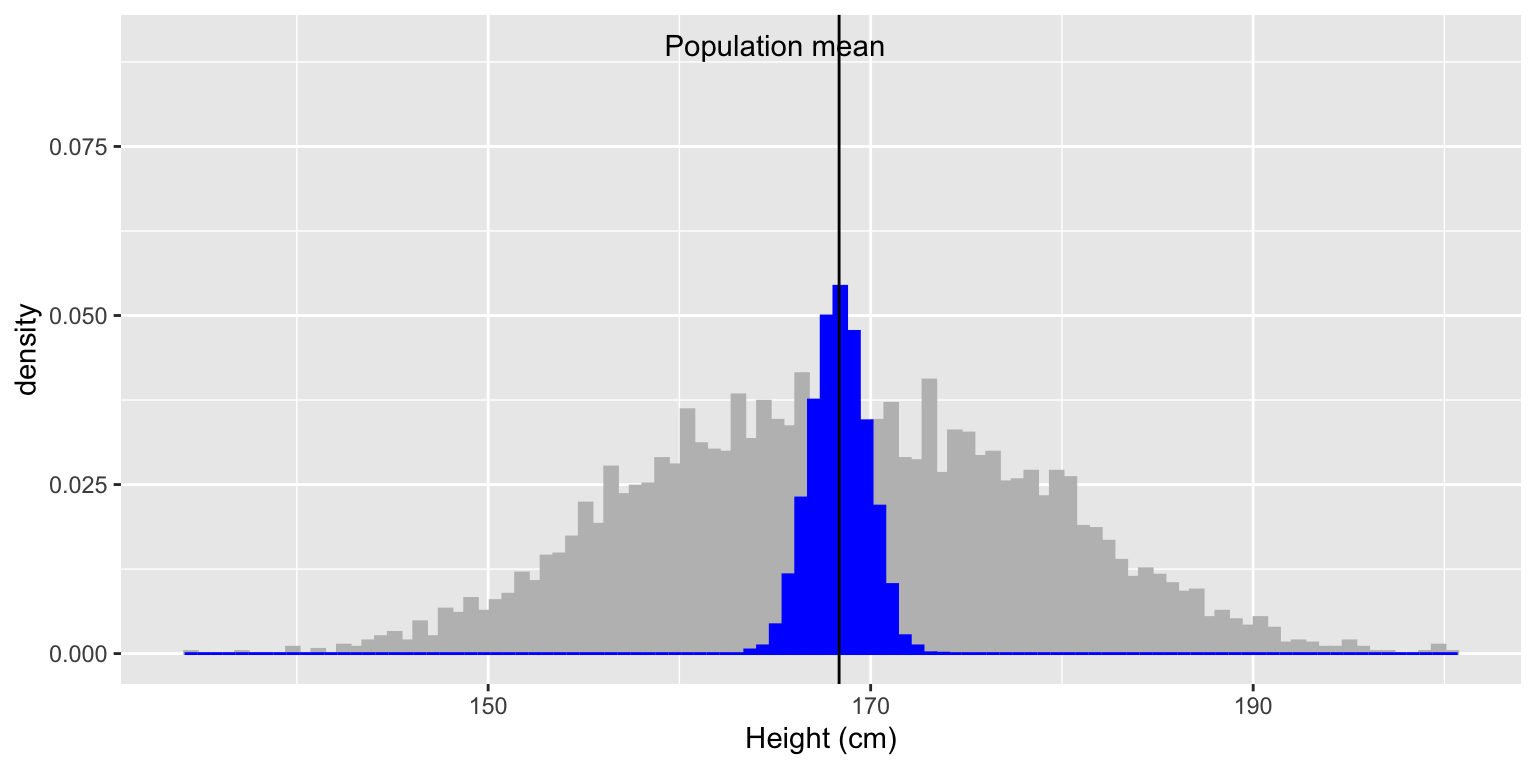
\includegraphics[height=0.5\textheight]{StatsThinking21_files/figure-latex/samplePlot-1} \caption{El histograma azul muestra la distribución muestral de la media de más de 5000 muestras aleatorias del conjunto de datos NHANES. El histograma del conjunto de datos completo se muestra en gris como referencia.}\label{fig:samplePlot}
\end{figure}

\hypertarget{standard-error-of-the-mean}{%
\section{Error estándar de la media}\label{standard-error-of-the-mean}}

Más adelante en el curso será esencial poder caracterizar qué tan variable son nuestras muestras, en orden para hacer inferencias sobre la estadística de la muestra. Para la media, hacemos esto utilizando una cantidad llamada \emph{error estándar} de la media (SEM por sus siglas en inglés), en la que podemos pensar como la desviación estándar de la distribución muestral. Para calcular el error estándar de la media para nuestra muestra, dividimos la estimada desviación estándar por la raíz cuadrada del tamaño de la muestra:

\[
SEM = \frac{\hat{\sigma}}{\sqrt{n}}
\]

Nota que tenemos que ser cuidadoses acerca de calcular el error estándar de la media utilizando la desviación estándar estimada si nuestra muestra es pequeña (\textless30).

Debido a que tenemos muchas muestras de la población NHANES y realmente conocemos el SEM de la población (que calculamos dividiendo la desviación estándar de la población por el tamaño de la población), podemos confirmar que el SEM que se calculó usando el parámetro de población (1.44) está muy cerca de la desviación estándar observada de las medias para las muestras que tomamos del conjunto de datos NHANES (1.43).

La fórmula para el error estándar de la media implica que la calidad de nuestra medición involucra dos cantidades: la variabilidad de la población y el tamaño de nuestra muestra. Dado que el tamaño de la muestra es el denominador en la fórmula de SEM, un tamaño de muestra más grande producirá un SEM más pequeño cuando se mantiene constante la variabilidad de la población. No tenemos control sobre la variabilidad de la población, pero \emph{sí} tenemos control sobre el tamaño de la muestra. Por lo tanto, si deseamos mejorar nuestras estadísticas muestrales (reduciendo su variabilidad muestral), entonces deberíamos utilizar muestras más grandes. Sin embargo, la fórmula también nos dice algo muy fundamental sobre el muestreo estadístico, a saber, que la utilidad de muestras más grandes disminuye con la raíz cuadrada del tamaño de la muestra. Esto significa que duplicar el tamaño de la muestra \emph{no} duplicará la calidad de las estadísticas; más bien, lo mejorará en un factor de \(\sqrt{2}\). En la Sección \ref{statistical-power} discutiremos la potencia estadística, que está íntimamente ligada a esta idea.

\hypertarget{the-central-limit-theorem}{%
\section{El teorema del límite central}\label{the-central-limit-theorem}}

El teorema del límite central nos dice que a medida que el tamaño de la muestra aumenta, la distribución muestral de la media se distribuirá normalmente, \emph{incluso si los datos dentro de cada muestra no se distribuyen normalmente}.

Primero, digamos un poco sobre la distribución normal. También se conoce como la distribución \emph{gaussiana}, en honor a Carl Friedrich Gauss, un matemático que no la inventó pero que jugó un papel en su desarrollo. La distribución normal se describe en términos de dos parámetros: la media (que puede considerar la ubicación del pico) y la distribución estándar (que especifica el ancho de la distribución). La forma de campana de la distribución nunca cambia, solo su ubicación y ancho. La distribución normal se observa comúnmente en los datos recopilados en el mundo real, como ya hemos visto en el capítulo 3, y el teorema del límite central nos da una idea de por qué ocurre eso.

Para ver el teorema del límite central en acción, trabajemos con la variable \(AlcoholYear\) del conjunto de datos NHANES, que está muy sesgada, como se muestra en el panel izquierdo de la Figura \ref{fig:alcDist50}. Esta distribución es, a falta de una palabra mejor, original, y definitivamente no se distribuye normalmente. Ahora veamos la distribución muestral de la media de esta variable. La figura \ref{fig:alcDist50} muestra la distribución muestral para esta variable, que se obtiene extrayendo repetidamente muestras de tamaño 50 del conjunto de datos NHANES y tomando la media. A pesar de la clara no normalidad de los datos originales, la distribución muestral es notablemente cercana a la normal.

\begin{figure}
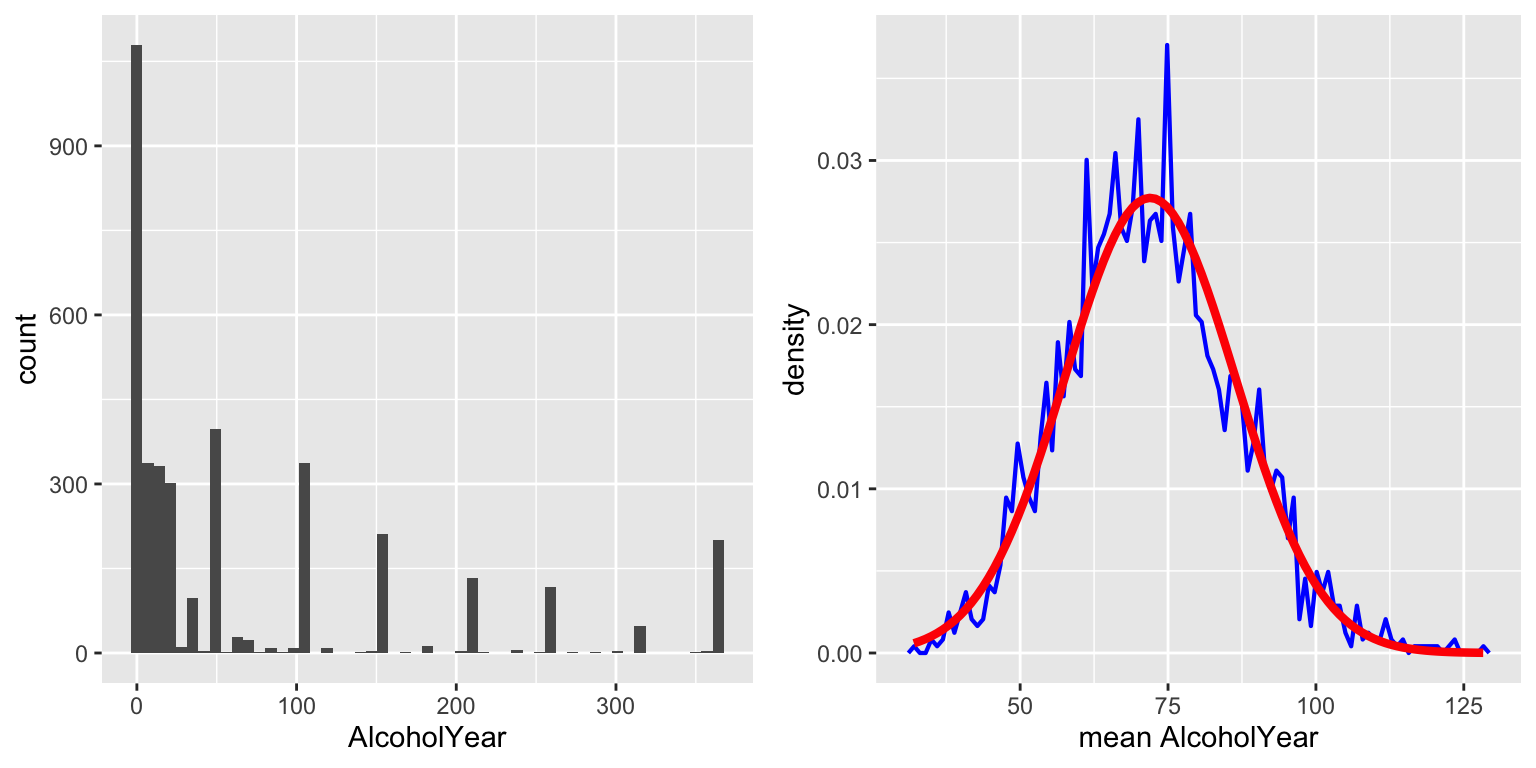
\includegraphics[height=0.5\textheight]{StatsThinking21_files/figure-latex/alcDist50-1} \caption{Izquierda: Distribución de la variable AlcoholYear en el conjunto de datos NHANES, la cual refleja el número de días que el individuo bebió en el año. Derecha: La distribución de muestreo de la media para AlcoholYear en el conjunto de datos NHANES, obtenido dibujando muestras repetidas de tamaño 50, en azul. La distribución normal con la misma media y la desviación estándar está mostrada en rojo.}\label{fig:alcDist50}
\end{figure}

El teorema de límite central es importante para la estadística porque nos permite asumir con seguridad que la distribución de muestreo de la media va a ser normal en la mayoría de los casos. Esto significa que podemos tomar ventaja de las técnicas estadísticas que asumen una distribución normal, como veremos en la próxima sección. Es también importante porque nos dice por qué las distribuciones normales son tan comunes en el mundo real; siempre que combinamos factores diferentes en un solo número, el resultado muy probablemente será una distribución normal. Por ejemplo, la altura de cualquier adulto depende en una compleja mexcla de su genética y experiencia; incluso si las contribuciones individuales pueden no ser normalmente distribuidas, cuando las combinemos el resultado es una distribución normal.

\hypertarget{confidence-intervals}{%
\section{Intervalos de confianza}\label{confidence-intervals}}

La mayoría de las personas están familiarizadas con la idea de un ``margen de error'' en encuestas políticas. Estas encuestas usualmente intentan proveer una respuesta que es más o menos 3\% precisa. Por ejemplo cuando un candidato es estimado a ganar la elección por 9\% de los puntos con un margen de error de 3, el porcentaje por el cual va a ganar es estimado a caer dentro del 6-12 porciento de puntos. En estadística nos referimos a este rango de valores como el \emph{intervalo de confianza}, el cual provee una medida por nuestro grado de incertidumbre sobre de qué tan cercano nuestro estimado particular basado en una única muestra está del parámetro poblacional. Entre más grande sea el intervalo de confianza, mayor es la incertidumbre.

Vimos en la sección previa que con una muestra suficiente en tamaño, la distribución de la media de muestreo está normalmente distribuida, y que el error estándar describe la desviación estándar de esta distribución de muestreo. Usando este conocimiento, podemos preguntarnos: ¿Cuál es el rango de valores con el cual podemos esperar capturar el 95\% de todos los estimados de la media? Para contestar esto, podemos usar la distribución normal, por la cual sabemos que los valores entre los cuales esperamos que caiga el 95\% de todas las medias muestrales; en software estadístico, nos referimos generalmente a estos como \emph{cuantiles}. Específicamente, necesitamos determinar el 2.5\% y 9.7\% cuantiles de la distribución. Elegimos estos puntos porque queremos encontrar el 95\% de los valores en el centro de la distribución, así que necesitamos cortar 2.5\% en cada extremo para así poder terminar con 95\% en el medio. La Figura \ref{fig:normalCutoffs} muestra que esto ocurre para \(Z \pm 1.96\).

\textbackslash begin\{figure\}
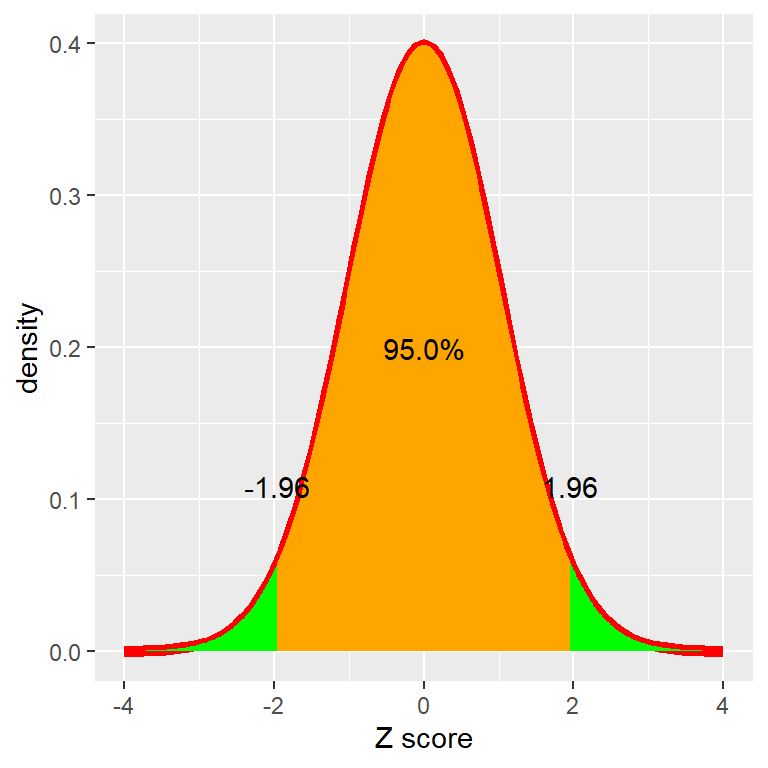
\includegraphics[height=0.5\textheight]{StatsThinking21_files/figure-latex/normalCutoffs-1} \textbackslash caption\{Distribución normal, con la sección anaranjada en el centro denotando el rango en el cual se espera el 95\% de todos los valores. La sección verde muestra las porciones de la distribución que están más al extremo, las cuales esperaríamos que ocurrieran menos de 5\% del tiempo.\}\label{fig:normalCutoffs}
\textbackslash end\{figure\}

Usando estos puntos de corte, podemos crear un intervalo de confianza para el estimado de la media:
\[
CI_{95\%} = \bar{X} \pm 1.96*SEM
\]
Calculemos el intervalo de confianza para los datos de altura de NHANES.

\begin{tabular}{r|r|r|r}
\hline
Sample mean & SEM & Lower bound of CI & Upper bound of CI\\
\hline
169 & 1.4 & 166 & 172\\
\hline
\end{tabular}

Los intervalos de confianza son notoriamente confusos, primeramente porque no significan lo que esperaríamos que significacen. Parece natural asumir que el 95\% intervalo de confianza nos dice que hay un 95\% de oportunidad de que la población esté dentro de ese intervalo. Sin embargo, como veremos a través del curso, los conceptos en estadística regularmente no significan lo que creemos que deberían significar. En el caso de los intervalos de confianza, no podemos interpretarlos en esta manera porque el parámetro poblacional tiene un valor fijo -- está o no está en el intervalo, por lo que no tiene sentido hablar de la probabilidad de que eso ocurra. La interpretación correcta del intervalo de confianza del 95\% es que es un intervalo que contendrá la media real de la población el 95\% del tiempo y, de hecho, podemos confirmarlo usando simulación. Aprenderemos más sobre los intervalos de confianza más adelante en el curso después de discutir la prueba de hipótesis.

\hypertarget{objetivos-de-aprendizaje-6}{%
\section{Objetivos de aprendizaje}\label{objetivos-de-aprendizaje-6}}

Al haber leído este capítulo, tu deberías de ser capaz de:

\begin{itemize}
\tightlist
\item
  Distinguir entre una población y una muestra, y entre parámetros de población y estadísticas de muestra
\item
  Describir los conceptos de error muestral y distribución muestral.
\item
  Calcular el error estándar de la media.
\item
  Describir cómo el teorema del límite central determina la naturaleza de la distribución muestral de la media.
\item
  Calcular un intervalo de confianza para la media basado en la distribución normal y describa su interpretación apropiada.
\end{itemize}

\hypertarget{lecturas-sugeridas-4}{%
\section{Lecturas sugeridas}\label{lecturas-sugeridas-4}}

\begin{itemize}
\tightlist
\item
  \emph{The Signal and the Noise: Why So Many Predictions Fail - But Some Don't}, by Nate Silver
\end{itemize}

\hypertarget{resampling-and-simulation}{%
\chapter{Remuestreo y Simulación}\label{resampling-and-simulation}}

El uso de las simulaciones a computadora se ha convertido en un aspecto esencial de la estadística moderna. Por ejemplo, uno de los libros más importantes en informática práctica se llama ``Recetas numéricas'', y recita lo siguiente:

\begin{quote}
``Si nos ofrecieran la opción entre tener el dominio de una estantería de cinco pies llena de libros de estadística y una mediana capacidad para realizar simulaciones estadísticas a lo Monte Carlo, seguramente elegiríamos la segunda opción.''
\end{quote}

En este capítulo hablaremos del concepto de una simulación Monte Carlo y discutiremos cómo puede ser usada para realizar análisis estadísticos.

\hypertarget{simulaciuxf3n-monte-carlo}{%
\section{Simulación Monte Carlo}\label{simulaciuxf3n-monte-carlo}}

El concepto de la simulación Monte Carlo fue ideada por los matemáticos Stan Ulam y Nicholas Metropolis, quienes estuvieron trabajando para desarrollar un arma atómica para los Estados Unidos de América, como parte del Proyecto Manhattan. Necesitaban calcular el promedio de la distancia que recorrería un neutrón en una sustancia antes de que chocara con un núcleo atómico, pero no pudieron calcular esto usando matemáticas estándar. Ulam notó que estos cálculos podían ser simulados usando números aleatorios, justo como un juego de casino. En un juego de casino, como la ruleta, los números son generados de manera aleatoria; para estimar la probabilidad de un resultado específico, uno podría jugar el juego cientos de veces. El tío de Ulam había jugado en el casino Monte Carlo en Monaco, de ahí viene el nombre para esta nueva técnica.

Hay cuatro pasos a seguir para realizar una simulación Montecarlo:

\begin{enumerate}
\def\labelenumi{\arabic{enumi}.}
\tightlist
\item
  Definir el dominio posible de los valores
\item
  Generar números al azar dentro de ese dominio a partir de una distribución de probabilidad
\item
  Realizar un cálculo usando números aleatorios
\item
  Combinar los resultados a través de muchas repeticiones
\end{enumerate}

Como un ejemplo, digamos que quiero descubrir cuánto tiempo debo dejar para un test en clase. Digamos que sabemos que la distribución del tiempo para completar el test es normal, con una media de 5 minutos y una desviación estándar de 1 minuto. Sabiendo esto, ¿qué tan largo debe ser el periodo de tiempo para que esperemos que todos los estudiantes terminen el examen el 99\% del tiempo? Hay dos formas de resolver este problema. El primero es calculando la respuesta usando una teoría matemática conocida como estadística de valores extremos. No obstante, esto requiere matemáticas complejas. De forma alternativa, podríamos usar el método de Montecarlo. Para hacer esto, necesitamos generar muestras aleatorias de una distribución normal.

\hypertarget{aleatoriedad-en-estaduxedstica}{%
\section{Aleatoriedad en Estadística}\label{aleatoriedad-en-estaduxedstica}}

El término ``aleatorio'' es usado coloquialmente para describir cosas que son bizarras o inesperadas, pero en estadística el término tiene un significado específico: Un proceso se considera \emph{aleatorio} si es impredecible. Por ejemplo, si lanzo una moneda 10 veces, el valor del resultado de una vez que la lances no va a predecir el resultado de la segunda vez que lo lances. Es importante destacar que el hecho de que algo es impredecible, no quiere decir que no es determinista. Por ejemplo, cuando lanzamos una moneda, el resultado de ésta está determinada por las leyes de la física; si supiéramos que todas las condiciones con suficiente detalle, podríamos predecir el resultado de cuando lancemos la moneda. De cualquier forma, son muchos factores los que se combinan para hacer el resultado del lanzamiento de la moneda impredecible en la práctica.

Lxs psicólogxs han demostrado que lxs humanxs tienen un sentido algo ineficiente para la aleatoriedad. En primera instancia, tendemos a ver patrones en donde no existen. De forma extrema, esto nos lleva al fenómeno de la \emph{pareidolia}, en el cual las personas tienden a percibir objetos familiares en patrones aleatorios (como ver una nube con una rostro humano, o ver a la Vírgen María en un pedazo de pan tostado). En segunda instancia, lxs humanxs tienden a pensar en procesos aleatorios como una forma de auto-corrección, lo cual nos lleva a creer que vamos a ganar después de varias rondas de perder un juego de azar, es un fenómeno llamada ``la falacia del jugador''.

\hypertarget{generando-nuxfameros-aleatorios}{%
\section{Generando números aleatorios}\label{generando-nuxfameros-aleatorios}}

Hacer correr una simulación con el método de Montecarlo requiere que generemos números aleatorios. Para generar números genuinamente aleatorios (por ejemplo, números que son completamente impredecibles) es solamente posible a través de procesos físicos, como decaimiento de átomos o el rodar unos dados, los cuales son difíciles de obtener o muy lentos como para que sean útiles en una simulación a computadora (aunque pueden obtenerse mediante \href{https://www.nist.gov/programs-projects/nist-randomness-beacon\%5D}{NIST Randomness Beacon}).

En general, en lugar de números verdaderamente aleatorios, podemos usar números \emph{pseudo-aleatorios}, generados utilizando un algoritmo de computadora; estos números pueden aparentar ser aleatorios en el sentido de que son difíciles de predecir, pero las series de números eventualmente se repetirán en algún punto. Por ejemplo, el generador de números aleatorios utilizados en R se repetirán después de \(2^{19937} - 1\) números. Eso es mucho más que el número de segundos en la historia de universo, y generalmente pensamos que esto funciona para la mayoría de los propósitos en análisis estadísticos.

La mayoría de los softwares estadísticos incluyen funciones para generar números aleatorios para cada una de las grandes probabilidades de distribuciones, tal como la distribución uniforme (todos los valores entre 0 y 1 son equitativos), la distribución normal y la distribución binominal (por ejemplo, echar los dados o lanzar una moneda). La Figura \ref{fig:rngExamples} muestra ejemplos de números generados a partir de funciones de distribución uniformes y normales.

\begin{figure}
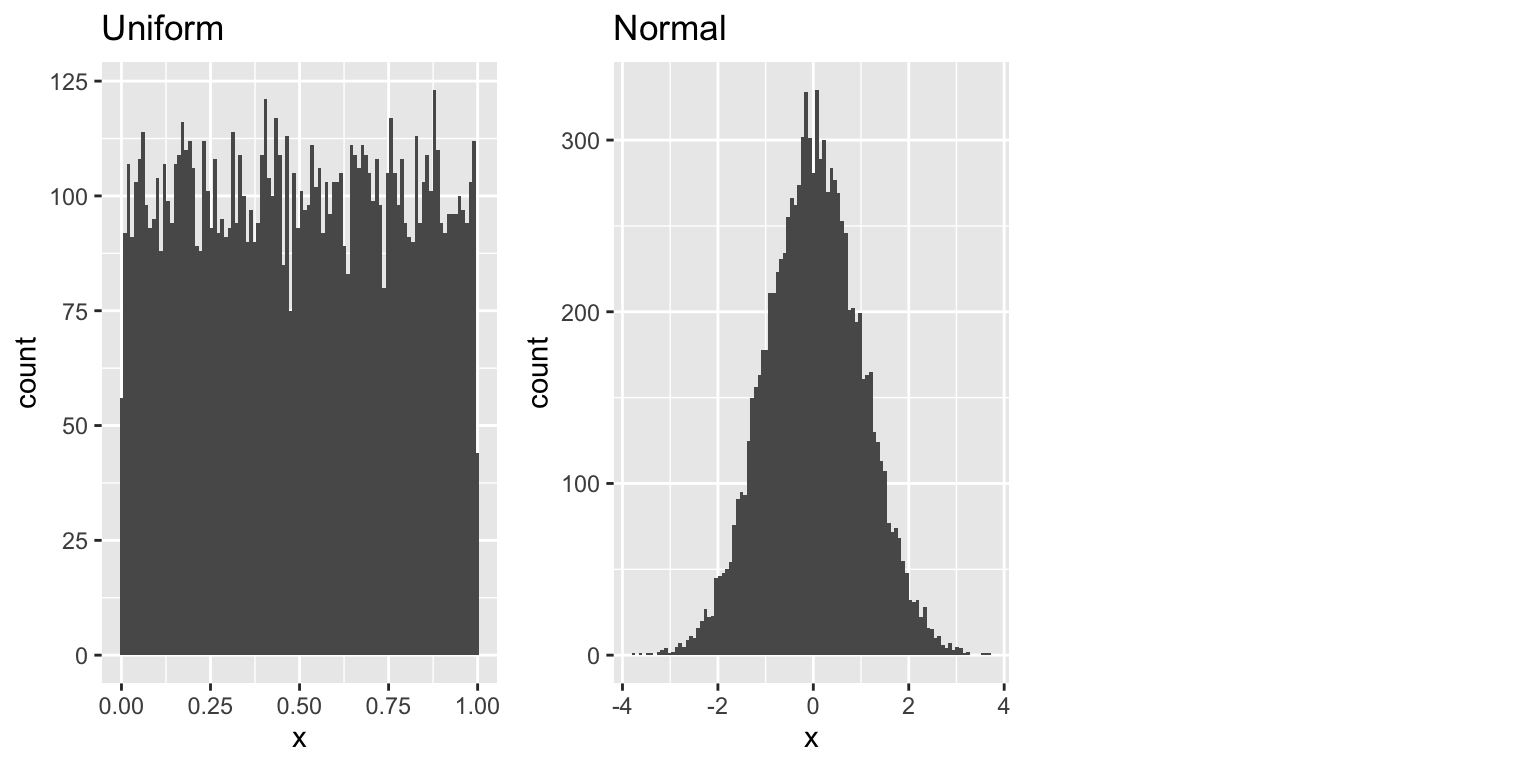
\includegraphics[height=0.5\textheight]{StatsThinking21_files/figure-latex/rngExamples-1} \caption{Examples of random numbers generated from a uniform (left) or normal (right) distribution.}\label{fig:rngExamples}
\end{figure}

Unx puede también generar números aleatorios por cualquier distribución utilizando una función de \emph{cuantil} para la distribución. Esto es lo inverso de la función de distribución cumulativa; en lugar de identificar las probabilidades cumulativas de un set de valores, la función de cuantiles identifica los valores para un set de probabilidades cumulativas. Usando la función de cuantiles, podemos generar números aleatorios de una distribución uniforme, y después mapearlos en la distribución de interés mediante su función de cuantil.

Por la forma en la que están creados, los generadores de números aleatorios en software estadísticos generan diferentes grupos de números aleatorios cada vez que los eches a correr. Sin embargo, también es posible que generen el mismo grupo de números aleatorios al configurar lo que se llama \emph{semilla aleatoria} (o por su nombre en inglés \emph{random seed}) a un valor específico. Haremos esto en muchos ejemplos en este libro, con el propósito de asegurarnos que los ejemplos son reproducibles.

\hypertarget{utilizando-una-simulaciuxf3n-con-el-muxe9todo-de-montecarlo}{%
\section{Utilizando una simulación con el Método de Montecarlo}\label{utilizando-una-simulaciuxf3n-con-el-muxe9todo-de-montecarlo}}

Regresemos a nuestro ejemplo sobre los tiempos de finalización de un examen. Dígamos que administro tres pruebas y grabo los tiempos en que cada alumno termina su examen, lo cual se vería como las distribuciones que se presentan en la Figura \ref{fig:finishingTimes}.

\begin{figure}
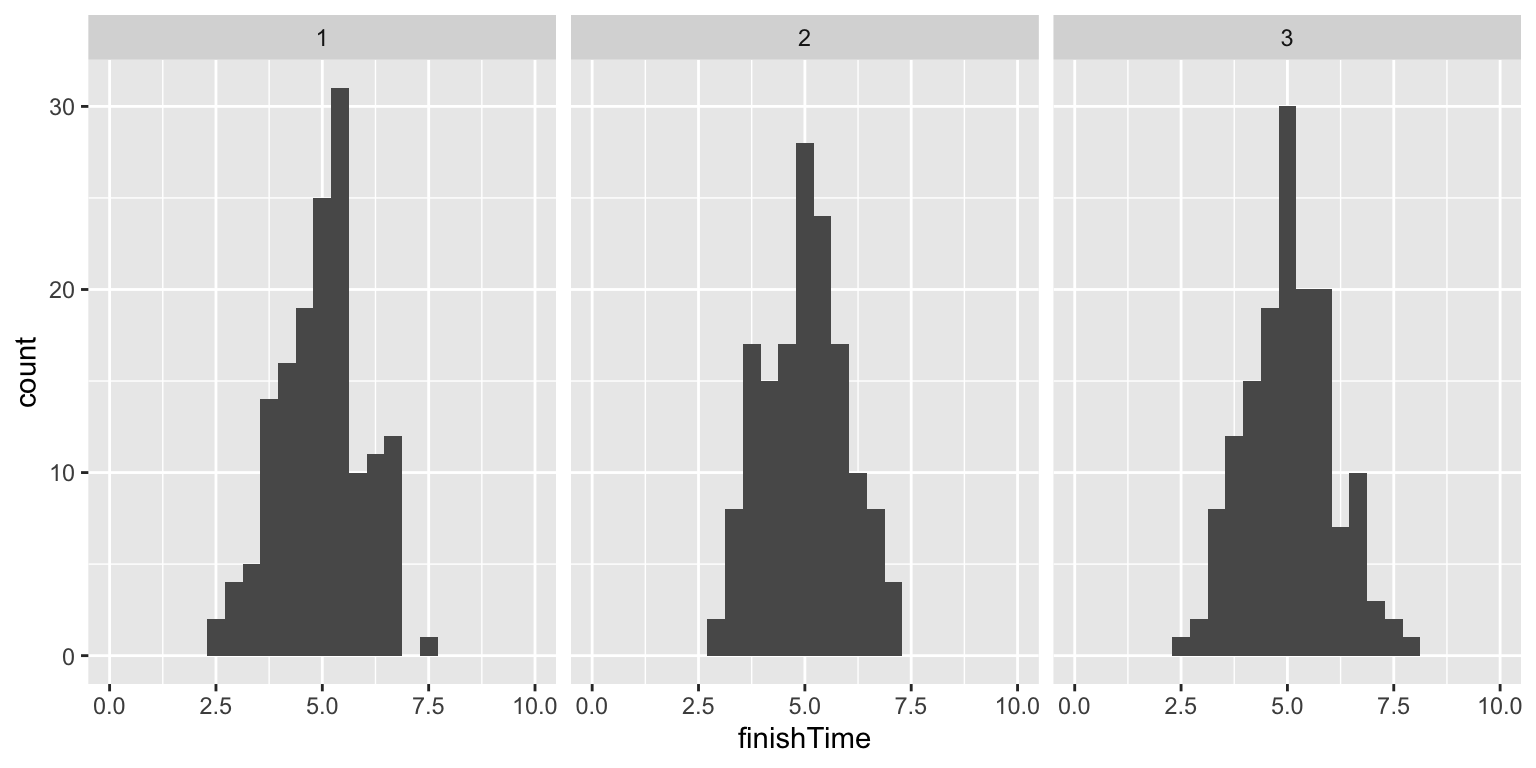
\includegraphics[height=0.5\textheight]{StatsThinking21_files/figure-latex/finishingTimes-1} \caption{Simulated finishing time distributions.}\label{fig:finishingTimes}
\end{figure}

Sin embargo, lo que realmente queremos saber no es cómo se ve la distribución de los tiempos de finalización del examen, sino más bien cómo se ve la distribución del tiempo \emph{más largo} de finalización de cada examen. Para hacer eso, podemos simular el tiempo de finalización para cada examen, asumiendo que los tiempos de finalización están distribuidos de forma normal, como hemos establecido arriba; para cada uno de estas simulaciones de examenes, después grabamos el tiempo más largo de finalización. Repetimos esta simulación un gran número de veces (5000 debería ser suficiente) y luego grabamos la distribución de los tiempos de finalización, lo cual se muestra en la Figura \ref{fig:finishTimeSim}.

\begin{figure}
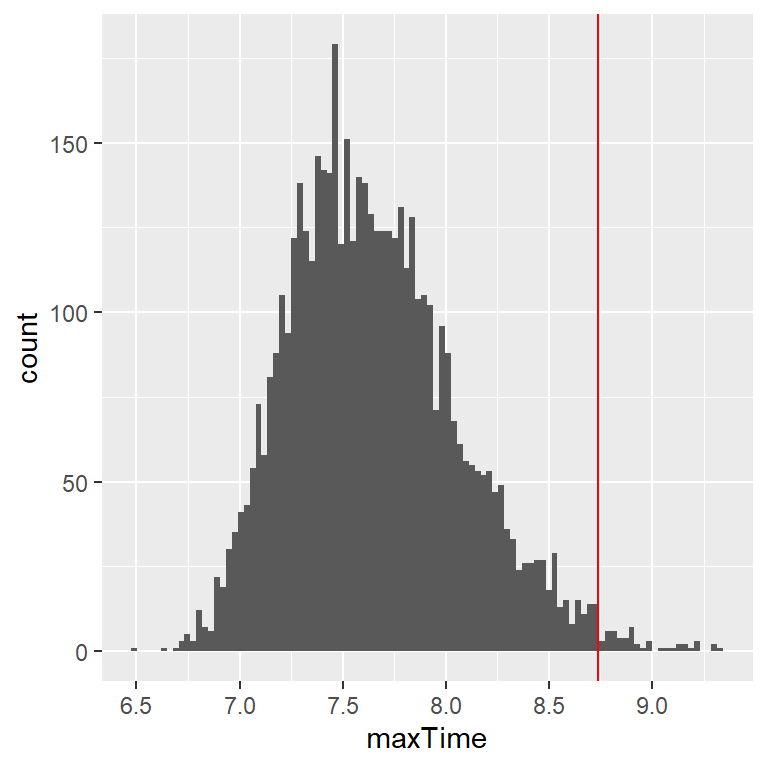
\includegraphics[height=0.5\textheight]{StatsThinking21_files/figure-latex/finishTimeSim-1} \caption{Distribution of maximum finishing times across simulations.}\label{fig:finishTimeSim}
\end{figure}

Esto muestra que el percentil número 99 de la distribución de la finalización del examen se encuentra en 8.74, lo cual significa que si diéramos esa cantidad de tiempo para el examen, entonces al menos el 99\% de personas deberían de terminar a tiempo. Siempre es importante recordar que nuestras suposiciones importan-- si están mal, entonces los resultados de la simulación serán inservibles. En este caso, asumimos que la distribución del tiempo de finalización estaba distribuido normalmente con una media en particular y una desviación estándar; si estas suposiciones son incorrectas (y casi siempre lo son), entonces la respuesta real podría ser muy diferente.

\hypertarget{usando-simulaciones-para-estaduxedstica-the-bootstrap}{%
\section{Usando simulaciones para estadística: The bootstrap}\label{usando-simulaciones-para-estaduxedstica-the-bootstrap}}

Hasta ahora hemos utilizado simulaciones para demostrar principios estadísticos, pero también podemos usar simulaciones para responder a preguntas estadísticas reales. En esta sección vamos a presentar un concepto conocido como el \emph{bootstrap} (por su nombre en inglés), este nos permite usar simulaciones para cuantificar la incertidumbre de estimaciones estadísticas. Más tarde en este curso, veremos otros ejemplos de cómo la simulación puede ser utilizada en muchas ocasiones para responder preguntas estadísticas, en especial, cuando los métodos de teoría estadística no están disponibles o sus suposiciones son muy difíciles de cumplir.

\hypertarget{calculando-el-bootstrap}{%
\subsection{Calculando el bootstrap}\label{calculando-el-bootstrap}}

En el capítulo anterior, utilizamos nuestro conocimiento del muestro de la distribución de la media para calcular el error estándar de la media y los intervalos de confianza. Pero ¿qué pasa si no podemos asumir que las estimaciones están distribuidas de forma normal, o si no sabemos su distribución? La idea del bootstrap es usar los mismos datos para estimar la respuesta. El nombre viene de la idea de levantarse a unx mismx por las cuerdas de sus propias botas, expresando la idea de que no necesitamos herramientas externas para utilizar como palanca, así que tenemos que asir de los mismos datos. El método boostrap fue acuñado por Bradley Efron en el Departamento de Estadística de Stanford, quien es uno de los estadísticos más influyentes del mundo.

La idea detrás del bootstrap es que repetidamente tomamos muestras del conjunto de datos real; lo que es más importante, muestreamos \emph{con reemplazo}, de modo que el mismo punto de datos a menudo terminará representado varias veces en una de las muestras. Después calculamos nuestro interés estadístico en cada una de las muestras del bootstrap, y utilizamos la distribución de esos estimados como nuestra distribución muestral.

Comencemos utilizando el bootstrap para estimar la distribución muestral de la media, para que podamos comparar el resultado del error estándar de la media (SEM, por sus siglas en inglés), que mencionamos hace unos momentos.

\begin{figure}
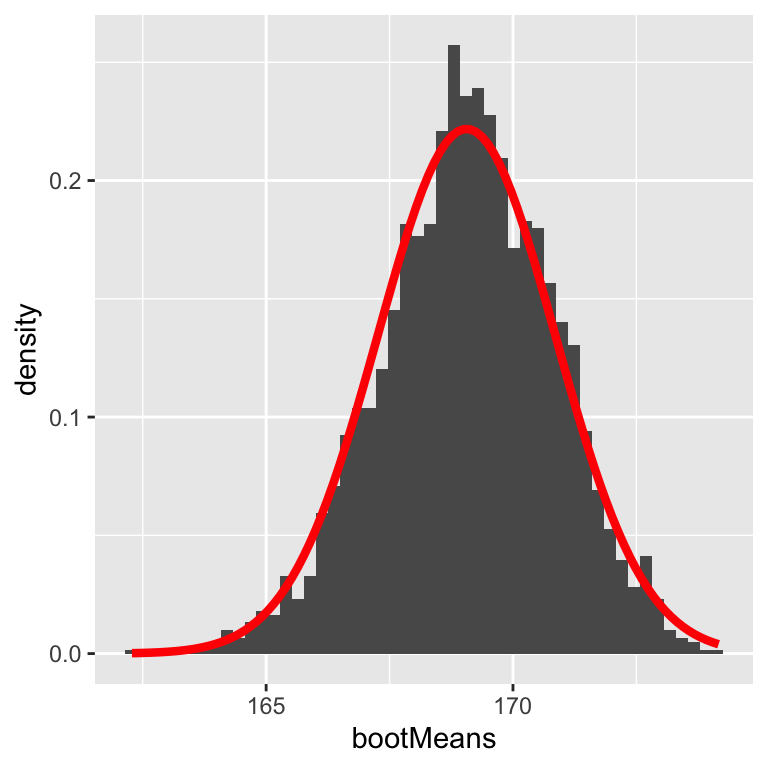
\includegraphics[height=0.5\textheight]{StatsThinking21_files/figure-latex/bootstrapSEM-1} \caption{An example of bootstrapping to compute the standard error of the mean. The histogram shows the distribution of means across bootstrap samples, while the red line shows the normal distribution based on the sample mean and standard deviation.}\label{fig:bootstrapSEM}
\end{figure}

La Figura \ref{fig:bootstrapSEM} muestra que la distribución de la media a través de las muestras del bootstrap es muy cercana al estimado teórico basado en la suposición de normalidad. También podemos usar las muestras de bootstrap para calcular un intervalo de confianza para la media, simplemente al calcular los cuantiles de interés de la distribución de las muestras del bootstrap.

\begin{table}

\caption{\label{tab:unnamed-chunk-37}Confidence limits for normal distribution and bootstrap methods}
\centering
\begin{tabular}[t]{l|r|r}
\hline
type & 2.5\% & 97.5\%\\
\hline
Normal & 166 & 173\\
\hline
Bootstrap & 166 & 172\\
\hline
\end{tabular}
\end{table}

Usualmente no utilizaríamos el bootstrap para calcular intervalos de confianza para la media (ya que, generalmente podemos asumir que la distribución normal es apropiada para la distribución muestral de la media, siempre y cuando nuestra muestra sea lo suficientemente grande), pero este ejemplo muestra que el método nos da un resultado aproximadamente igual al método estándar basado en distribución normal. El bootstrap es más comunmente utilizado para generar errores estándar para estimaciones de otras estadísticas, en donde sabemos o sospechamos que la distribución normal no es apropiada.

\hypertarget{objetivos-de-aprendizaje-7}{%
\section{Objetivos de aprendizaje}\label{objetivos-de-aprendizaje-7}}

Después de haber leído este capítulo, deberías ser capaz de:

\begin{itemize}
\tightlist
\item
  Describir el concepto del método de Montecarlo.
\item
  Describir el significado de la aleatoriedad en estadística.
\item
  Describir cómo son generados los números pseudo-aleatorios.
\item
  Describir el concepto de bootstrap.
\end{itemize}

\hypertarget{lecturas-sugeridas-5}{%
\section{Lecturas sugeridas}\label{lecturas-sugeridas-5}}

\begin{itemize}
\tightlist
\item
  \emph{Computer Age Statistical Inference: Algorithms, Evidence and Data Science}, by Bradley Efron and Trevor Hastie.
\end{itemize}

\hypertarget{hypothesis-testing}{%
\chapter{Prueba de hipótesis}\label{hypothesis-testing}}

En el primer capítulo discutimos los tres grandes objetivos de la estadística:

\begin{itemize}
\tightlist
\item
  Describir
\item
  Decidir
\item
  Predecir
\end{itemize}

En este capítulo presentaremos las ideas detrás del uso de la estadística para tomar decisiones -- en particular, decisiones acerca de si una hipótesis en particular es apoyada por los datos.

\hypertarget{prueba-estaduxedstica-de-hipuxf3tesis-nula-null-hypothesis-statistical-testing-nhst}{%
\section{Prueba Estadística de Hipótesis Nula (Null Hypothesis Statistical Testing, NHST)}\label{prueba-estaduxedstica-de-hipuxf3tesis-nula-null-hypothesis-statistical-testing-nhst}}

El tipo específico de prueba de hipótesis que discutiremos es conocido como (por razones que serán claras más adelante) \emph{prueba estadística de hipótesis nula} (\emph{null hypothesis statistical testing}, NHST). Si tomaras casi cualquier publicación científica o biomédica, verías la NHST siendo usada para probar hipótesis, y en su libro de texto de introducción a la psicología, Gerrig \& Zimbardo (2002) se refirieron a la NHST como el ``pilar de la investigación psicológica''. Por lo tanto, aprender cómo usar e interpretar los resultados de la prueba de hipótesis es esencial para entender los resultados de muchos campos de investigación.

También es importante que sepas, sin embargo, que la NHST tiene serias fallas, y muchos estadísticos e investigadores (incluyéndome) piensan que esto ha sido la causa de problemas serios en la ciencia, que discutiremos en el Capítulo \ref{doing-reproducible-research}. Por más de 50 años, ha habido llamados para abandonar la NHST en favor de otras aproximaciones (como aquellas que discutiremos en los siguientes capítulos):

\begin{itemize}
\tightlist
\item
  ``The test of statistical significance in psychological research may be taken as an instance of a kind of essential mindlessness in the conduct of research'' (Bakan, 1966)
\item
  Hypothesis testing is ``a wrongheaded view about what constitutes scientific progress'' (Luce, 1988)
\end{itemize}

NHST también es ampliamente malentendida, en gran medida porque va contra nuestras intuiciones acerca de cómo debería funcionar una prueba estadística de hipótesis. Veamos un ejemplo para observar esto.

\hypertarget{prueba-estaduxedstica-de-hipuxf3tesis-nula-un-ejemplo}{%
\section{Prueba estadística de hipótesis nula: Un ejemplo}\label{prueba-estaduxedstica-de-hipuxf3tesis-nula-un-ejemplo}}

Hay un gran interés en el uso de cámaras llevadas en el cuerpo por oficiales de policía, que se piensa que reducen el uso de la fuerza y mejoran el comportamiento del oficial. Sin embargo, para poder establecer esto necesitamos evidencia experimental, y se ha vuelto cada vez más común que los gobiernos usen ensayos controlados aleatorizados (randomized control trials) para probar este tipo de ideas. Un ensayo controlado aleatorizado de la efectividad del uso de cámaras en el cuerpo fue realizado por el gobierno de Washington, DC, y el DC Metropolitan Police Department en 2015/2016 para probar la hipótesis de si las cámaras llevadas en el cuerpo son efectivas. Los oficiales fueron asignados de manera aleatoria a usar cámaras en el cuerpo o no, y su comportamiento fue seguido por un tiempo para determinar si las cámaras resultaron en menor uso de la fuerza y menos quejas de civiles acerca del comportamiento del oficial.

Antes de que lleguemos a los resultados, preguntémonos cómo piensas que el análisis estadístico debería funcionar. Digamos que queremos específicamente probar la hipótesis de si el uso de la fuerza disminuye por el uso de las cámaras. El ensayo controlado aleatorizado nos provee con los datos para probar la hipótesis -- concretamente, la frecuencia de uso de la fuerza por oficiales asignados ya sea al grupo de cámara o al grupo control. El siguiente paso obvio es mirar los datos y determinar si proveen evidencia convincente a favor o en contra de esta hipótesis. Esto es: ¿Cuál es la probabilidad de que las cámaras usadas en el cuerpo reduzcan el uso de la fuerza, dados los datos y todo lo demás que sabemos?

Resulta que esta \emph{no} es la manera en que funciona la prueba de hipótesis nula. En su lugar, primero tomamos nuestra hipótesis de interés (i.e.~que las cámaras usadas en el cuerpo reducen el uso de la fuerza), y la volteamos de cabeza, creando una \emph{hipótesis nula} -- en este caso, la hipótesis nula sería que las cámaras no reducen el uso de la fuerza. De manera importante, luego de esto asumimos que la hipótesis nula es verdadera. Después miramos los datos, y determinamos qué tan probable serían estos datos si la hipótesis nula fuera cierta. Si los datos son los suficientemente improbables bajo la hipótesis nula, entonces podemos rechazar la nula en favor de la \emph{hipótesis alternativa} que es nuestra hipótesis de interés. Si no hay suficiente evidencia para rechazar la nula, entonces decimos que ``fallamos en rechazar'' la nula, y nos quedamos con nuestra suposición inicial de que la nula es cierta.

El entender algunos de los conceptos de NHST, particularmente el notable ``valor p'', es invariablemente desafiante la primera vez que uno se encuentra con ellos, porque son tan contra-intuitivos. Como veremos después, existen otras aproximaciones que proveen maneras más intuitivas para abordar la prueba de hipótesis (pero tienen sus propias complejidades). Sin embargo, antes de que lleguemos a esas, es importante que tengas una comprensión profunda de cómo funciona la prueba de hipótesis, porque claramente no se irá a ningún lado pronto.

\hypertarget{el-proceso-de-la-prueba-de-hipuxf3tesis-nula}{%
\section{El proceso de la prueba de hipótesis nula}\label{el-proceso-de-la-prueba-de-hipuxf3tesis-nula}}

Podemos descomponer el proceso de la prueba de hipótesis nula en un número de pasos:

\begin{enumerate}
\def\labelenumi{\arabic{enumi}.}
\tightlist
\item
  Formula una hipótesis que represente nuestra predicción (\emph{antes de ver los datos}).
\item
  Especifica las hipótesis nula y alternativa.
\item
  Recolecta datos relevantes para la hipótesis.
\item
  Ajusta el modelo a los datos que representen la hipótesis laternativa y calcula un estadístico de prueba.
\item
  Calcula la probabilidad del valor observado de ese estadístico asumiendo que la hipótesis nula es verdadera.
\item
  Evalúa la ``significatividad estadística'' del resultado.
\end{enumerate}

Para un ejemplo práctico, usemos la base de datos NHANES para hacernos la siguiente pregunta: ¿La actividad física está relacionada con el índice de masa corporal? En NHANES, los participantes respondieron si se involucran regularmente en deportes moderados o de intensidad vigorosa, fitness, o actividades recreativas (guardado en la variable \(PhysActive\)). Los investigadores también midieron la altura y el peso y los usaron para calcular el \emph{Índice de Masa Corporal} (IMC, o BMI por el término en inglés \emph{Body Mass Index}):

\[
BMI = \frac{weight(kg)}{height(m)^2}
\]

\hypertarget{paso-1-formular-una-hipuxf3tesis-de-interuxe9s}{%
\subsection{Paso 1: Formular una hipótesis de interés}\label{paso-1-formular-una-hipuxf3tesis-de-interuxe9s}}

Hipotetizamos que el IMC es mayor en las personas que no se involucran en actividades físicas, comparado con aquellas que sí lo hacen.

\hypertarget{paso-2-especifica-las-hipuxf3tesis-nula-y-alternativa}{%
\subsection{Paso 2: Especifica las hipótesis nula y alternativa}\label{paso-2-especifica-las-hipuxf3tesis-nula-y-alternativa}}

Para el paso 2, necesitamos especificar nuestra hipótesis nula (que llamaremos \(H_0\)) y nuestra hipótesis alternativa (que llamaremos \(H_A\)). \(H_0\) es la línea base contra la que probamos nuestra hipótesis de interés: esto es, ¿cómo esperaríamos que se vieran los datos si no hubiera un efecto? La hipótesis nula siempre involucra algún tipo de igualdad (=, \(\le\), o \(\ge\)). \(H_A\) describe lo que esperaríamos si realmente hubiera un efecto. La hipótesis alternativa siempre involucra algún tipo de diferencia/desigualdad (\(\ne\), \textgreater, o \textless). De manera importante, la prueba de hipótesis nula opera bajo la suposición de que la hipótesis nula es verdadera a menos que la evidencia demuestre lo contrario.

También tenemos que decidir si queremos probar una hipótesis \emph{direccional} o \emph{no direccional}. Una hipótesis no direccional simplemente predice que habrá una diferencia, sin predecir en qué dirección irá. Para el ejemplo de IMC/actividad, una hipótesis nula no direccional sería:

\(H0: BMI_{active} = BMI_{inactive}\)

y la correspondiente hipótesis alternativa no direccional sería:

\(HA: BMI_{active} \neq BMI_{inactive}\)

Una hipótesis direccional, por otro lado, predice en qué dirección irá la diferencia. Por ejemplo, tenemos conocimiento previo fuerte para predecir que la gente que se involucre en actividad física debería pesar menos que aquellos que no lo hacen, por lo tanto podríamos proponer la siguiente hipótesis nula direccional:

\(H0: BMI_{active} \ge BMI_{inactive}\)

y la alternativa direccional:

\(HA: BMI_{active} < BMI_{inactive}\)

Como veremos más tarde, probar una hipótesis no direccional es más conservador, por lo que esto es lo que generalmente se prefiere a menos que haya alguna razón fuerte \emph{a priori} para hipotetizar un efecto en una dirección en particular. ¡Las hipótesis, incluyen si son direccionales o no, siempre deberán ser especificadas antes de ver los datos!

\hypertarget{paso-3-recolectar-datos}{%
\subsection{Paso 3: Recolectar datos}\label{paso-3-recolectar-datos}}

En este caso, seleccionaremos una muestra de 250 individuos de la base de datos NHANES. La Figura \ref{fig:bmiSample} muestra un ejemplo de esa muestra, con el IMC mostrado separando los individuos activos e inactivos.

\begin{table}

\caption{\label{tab:unnamed-chunk-39}Resumen de datos de IMC para individuos activos vs inactivos}
\centering
\begin{tabular}[t]{l|r|r|r}
\hline
PhysActive & N & mean & sd\\
\hline
No & 131 & 30 & 9.0\\
\hline
Yes & 119 & 27 & 5.2\\
\hline
\end{tabular}
\end{table}

\begin{figure}
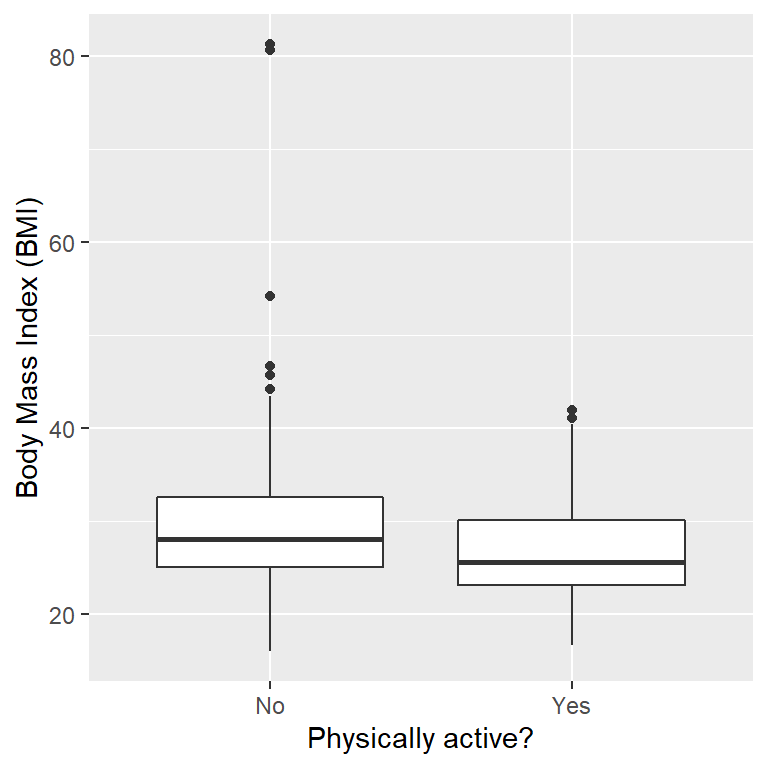
\includegraphics[height=0.5\textheight]{StatsThinking21_files/figure-latex/bmiSample-1} \caption{Gráfica de caja (boxplot) de los datos de IMC de una muestra de adultos de NHANES, divididos según reportaron involucrarse en actividad física regular.}\label{fig:bmiSample}
\end{figure}

\hypertarget{paso-4-ajusta-un-modelo-a-los-datos-y-calcula-el-estaduxedstico-de-prueba}{%
\subsection{Paso 4: Ajusta un modelo a los datos y calcula el estadístico de prueba}\label{paso-4-ajusta-un-modelo-a-los-datos-y-calcula-el-estaduxedstico-de-prueba}}

Después queremos usar los datos para calcular un estadístico que ultimadamente nos permitirá decidir si la hipótesis nula es rechazada o no. Para hacer esot, el modelo necesita cuantificar la cantidad de evidencia en favor de la hipótesis alternativa, relativa a la variabilidad en los datos. Por lo que podemos pensar en el estadístico de prueba como el que provee una medida del tamaño del efecto comparado con la variabilidad en los datos. En general, este estadístico de prueba tendrá una distribución de probabilidad asociada con él, porque eso nos permitirá determinar qué tan probable es nuestro valor estadístico observado bajo la hipótesis nula.

Para el ejemplo de IMC, necesitamos un estadístico de prueba que nos permita probar si hay una diferencia entre dos medias, puesto que las hipótesis están elaboradas en términos de la media de IMC en cada grupo. Un estadístico que es frecuentemente usado para comparar dos medias es el estadístico \emph{t}, desarrollado primero por el estadístico William Sealy Gossett, quien trabajó para la Guiness Brewery en Dublín y escribió bajo el pseudónimo ``Student'' - por eso, es frecuentemente llamada ``estadístico \emph{t} de Student''. El estadístico \emph{t} es apropiado para comparar las medias de dos grupos cuando los tamaños de muestra son relativamente pequeños y la desviación estándar de la población es desconocida. El estadístico \emph{t} para comparar dos grupos independientes es calculado de la siguiente manera:

\[
t = \frac{\bar{X_1} - \bar{X_2}}{\sqrt{\frac{S_1^2}{n_1} + \frac{S_2^2}{n_2}}}
\]

donde \(\bar{X}_1\) y \(\bar{X}_2\) son las medias de los dos grupos, \(S^2_1\) y \(S^2_2\) son las varianzas estimadas de los grupos, y \(n_1\) y \(n_2\) son los tamaños de cada grupo. Nota que el denominador es básicamente un promedio del error estándar de la media de las dos muestras. Por lo tanto, uno puede ver al estadístico \emph{t} como una manera de cuantificar qué tan grande es la diferencia entre grupos en relación con la variabilidad muestral de las medias que están siendo comparadas.

El estadístico \emph{t} se distribuye de acuerdo a una distribución de probabilidad conocida como distribución \emph{t}. La distribución \emph{t} se mira muy similar a una distribución normal, pero difiere dependiendo del número de grados de libertad (degrees of freedom), que para nuestro ejemplo es el número de observaciones menos 2, porque hemos calculado dos medias y por lo tanto hemos renunciado a dos grados de libertad. Cuando la cantidad de grados de libertad es grande (digamos 1,000), entonces la distribución \emph{t} se mira esencialmente como una distribución normal, pero cuando es pequeña entonces la distribución \emph{t} tiene colas más largas que la normal (ve la Figura \ref{fig:tVersusNormal}).

\begin{figure}
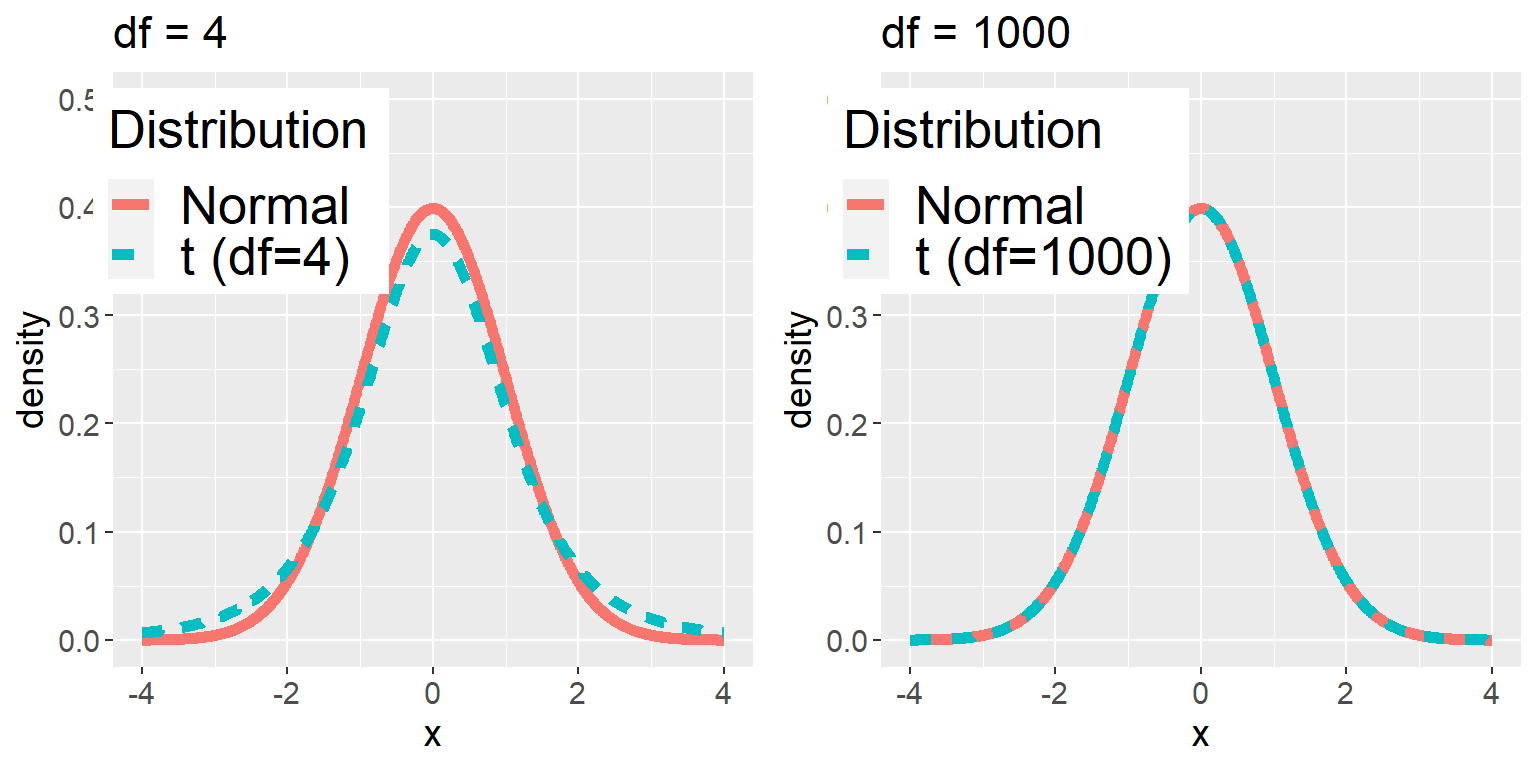
\includegraphics[height=0.5\textheight]{StatsThinking21_files/figure-latex/tVersusNormal-1} \caption{Cada panel muestra la distribución t (la línea azul punteada) sobrepuesta a la distribución normal (la línea roja continua). El panel izquierdo muestra una distribución t con 4 grados de libertad, en cuyo caso la distribución es similar pero tiene colas ligeramente más anchas. El panel derecho muestra una distribución t con 1000 grados de libertad, en cuyo caso es virtualmente idéntica a la normal.}\label{fig:tVersusNormal}
\end{figure}

\hypertarget{paso-5-determinar-la-probabilidad-de-los-datos-bajo-la-hipuxf3tesis-nula}{%
\subsection{Paso 5: Determinar la probabilidad de los datos bajo la hipótesis nula}\label{paso-5-determinar-la-probabilidad-de-los-datos-bajo-la-hipuxf3tesis-nula}}

Este es el paso donde la NHST comienza a ir contra nuestra intuición -- en lugar de determinar la probabilidad de que la hipótesis nula sea cierta dados los datos obtenidos, en su lugar determinamos la probabilidad de los datos bajo la hipótesis nula - ¡porque comenzamos los pasos asumiendo que la hipótesis nula es verdadera! Para hacer esto, necesitamos conocer la distribución de probabilidad del estadístico bajo la hipótesis nula, de tal manera que podamos preguntar qué tan probables son los datos bajo esa distribución. Podemos obtener esta ``distribución nula'' ya sea usando una distribución teórica (como la distribución \emph{t}), o usando aleatorización. Antes de movernos al ejemplo de IMC, comencemos con unos ejemplos más sencillos.

\hypertarget{randomization-very-simple}{%
\subsubsection{Aleatorización: Un ejemplo muy sencillo}\label{randomization-very-simple}}

Digamos que queremos determinar si una moneda está balanceada (que no esté trucada). Para recolectar datos, lanzamos la moneda 100 veces, y digamos que contamos 70 caras. En este ejemplo, \(H_0: P(cara)=0.5\) y \(H_A: P(cara) \neq 0.5\), y nuestro estadístico de prueba es simplemente el número de caras que contamos. La pregunta que entonces queremos hacernos es: ¿Qué tan probable es que hubiéramos observado 70 caras en 100 lanzamientos de moneda si la probabilidad verdadera de obtener cara es 0.5? Podríamos imaginar que esto podría suceder muy ocasionalmente sólo por azar, pero no parece muy probable. Para cuantificar esta probabilidad, podemos usar la \emph{distribución binomial}:

\[
P(X \le k) = \sum_{i=0}^k \binom{N}{k} p^i (1-p)^{(n-i)}
\]
Esta ecuación nos dirá la probabilidad de tener un cierto número de caras o menos, dada una probabilidad en particular de obtener cara y un número de eventos. Sin embargo, lo que realmente queremos saber es la probabilidad de un cierto número o más, que podemos obtener restando el resultado de uno, basados en las reglas de probabilidad:

\[
P(X \ge k) = 1 - P(X < k)
\]

\begin{figure}
\includegraphics[height=0.5\textheight]{StatsThinking21_files/figure-latex/coinFlips-1} \caption{Distribución de cantidad de caras (de un total de 100 lanzamientos) a lo largo de 100,000 simulaciones  con el valor de 70 representado por la línea vertical.}\label{fig:coinFlips}
\end{figure}

Usando la distribución binomial, la probabilidad de 69 o menos caras dado P(cara)=0.5 es 0.999961, por lo tanto la probabilidad de 70 o más caras es simplemente uno menos ese valor (0.000039).
Este cálculo nos muestra que la probabilidad de obtener 70 caras si la moneda efectivamente estuviera balanceada (no trucada) es muy pequeña.

Ahora, ¿qué pasaría si no tuviéramos una función estándar que nos dijera la probabilidad de ese número de caras? Entonces podríamos determinarla por medio de una simulación -- repetidamente lanzar la moneda 100 veces usando una probabilidad verdadera de 0.5, y luego calcular la distribución del número de caras a lo largo de estas simulaciones. La Figura \ref{fig:coinFlips} muestra el resultado de esta simulación. Aquí podemos ver que la probabilidad calculada a través de simulación (0.000030) es muy cercana a la probabilidad teórica (.00004).

Hagamos el cálculo análogo para nuestro ejemplo de IMC/actividad. Primero, calculamos el estadístico \emph{t} usando los valores de nuestra muestra que calculamos arriba, donde encontramos que t = 3.86. La pregunta que entonces queremos hacernos es: ¿Cuál es la probabilidad de que encontráramos un estadístico \emph{t} de este tamaño, si la diferencia verdadera entre grupos fuera cero o menor (i.e.~la dirección de la hipótesis nula)?

Podemos usar la distribución \emph{t} para determinar esta probabilidad. Nuestro tamaño de muestra es 250, por lo que la distribución \emph{t} apropiada tiene 248 grados de libertad porque perdemos un grado de libertad por cada una de las dos medias que calculamos. Podemos usar una función de nuestro software estadístico para determinar la probabilidad de encontrar un valor del estadístico \emph{t} mayor o igual al observado en nuestra muestra. Encontramos que p(t \textgreater{} 3.86, df = 248) = 0.000072, que nos dice que el valor estadístico \emph{t} observado de 3.86 es relativamente improbable si la hipótesis nula realmente fuera cierta.

En este caso, usamos una hipótesis direccional, por eso sólo tuvimos que observar un lado de la distribución nula. Si hubiéramos querido probar una hipótesis no direccional, entonces tendríamos que haber identificado qué tan inesperado es el tamaño del efecto, sin importar la dirección. En el contexto de la prueba t, eso significa que debemos saber qué tan probable es que el estadístico fuera tan extremo tanto en la dirección positiva como en la negativa. Para hacer esto, multiplicamos el valor \emph{t} observado por -1, porque la distribución \emph{t} está centrada alrededor de cero, y luego sumamos juntas las probabilidades de ambas colas para obtener un valor p de \emph{dos colas} (\emph{two-tailed}): p(t \textgreater{} 3.86 or t\textless{} -3.86, df = 248) = 0.000144. Aquí vemos que el valor p para la prueba de dos colas es el doble que para la prueba de una cola, esto refleja el hecho de que un valor extremo es menos sorpresivo porque podría haber ocurrido en cualquier dirección.

¿Cómo eliges si usar una prueba de una cola o de dos colas? La prueba de dos colas siempre será más conservadora, por lo que es una buena apuesta usar esa, a menos que ya tuvieras de antemano una razón fuerte previa para usar una prueba de una cola. En ese caso, tendrías que haber escrito la hipótesis antes de haber visto los datos. En el Capítulo \ref{doing-reproducible-research} discutiremos la idea del pre-registro de hipótesis, que formaliza la idea de escribir tus hipótesis antes de siquiera haber visto los datos reales. \emph{Nunca} deberías tomar una decisión acerca de cómo elaborar la hipótesis después de haber visto los datos, porque esto puede introducir sesgos serios en tus resultados.

\hypertarget{calcular-valores-p-usando-aleatorizaciuxf3n}{%
\subsubsection{Calcular valores p usando aleatorización}\label{calcular-valores-p-usando-aleatorizaciuxf3n}}

Hasta ahora, hemos visto cómo podemos usar la distribución t para calcular la probabilidad de los datos bajo la hipótesis nula, pero también podemos hacer esto usando simulaciones. La idea básica es que generemos datos simulados similares a los que esperaríamos bajo la hipótesis nula, y luego preguntarnos qué tan extremo es el dato observado en comparación con esos datos simulados. La pregunta clave es: ¿Cómo podemos generar datos para los cuales la hipótesis nula es verdadera? La respuesta general es que podemos reordenar nuestros datos de manera aleatoria en una manera particular que haga que los datos se vean como se deberían ver si la nula fuera realmente verdadera. Esto es similar a la idea de \emph{bootstrapping}, en el sentido de que usa nuestros propios datos para obtener una respuesta, pero lo hace de una manera diferente.

\hypertarget{aleatorizaciuxf3n-un-ejemplo-simple}{%
\subsubsection{Aleatorización: un ejemplo simple}\label{aleatorizaciuxf3n-un-ejemplo-simple}}

Comencemos con un ejemplo simple. Digamos que queremos comparar la habilidad promedio de hacer sentadillas de jugadores de football contra corredores de campo (\emph{cross-country runners}), con \(H_0: \mu_{FB} \le \mu_{XC}\) y \(H_A: \mu_{FB} > \mu_{XC}\). Medimos la habilidad máxima de hacer sentadillas de 5 jugadores de football y de 5 corredores de campo (que generaremos aleatoriamente, asumiendo que \(\mu_{FB} = 300\), \(\mu_{XC} = 140\), and \(\sigma = 30\)).

\begin{table}

\caption{\label{tab:squatPlot}Squatting data for the two groups}
\centering
\begin{tabular}[t]{l|r}
\hline
group & squat\\
\hline
FB & 265\\
\hline
FB & 310\\
\hline
FB & 335\\
\hline
FB & 230\\
\hline
FB & 315\\
\hline
XC & 155\\
\hline
XC & 125\\
\hline
XC & 125\\
\hline
XC & 125\\
\hline
XC & 115\\
\hline
\end{tabular}
\end{table}

\begin{table}

\caption{\label{tab:squatPlot}Squatting data after randomly scrambling group labels}
\centering
\begin{tabular}[t]{r|l}
\hline
squat & scrambledGroup\\
\hline
265 & XC\\
\hline
310 & FB\\
\hline
335 & XC\\
\hline
230 & FB\\
\hline
315 & XC\\
\hline
155 & FB\\
\hline
125 & XC\\
\hline
125 & XC\\
\hline
125 & FB\\
\hline
115 & FB\\
\hline
\end{tabular}
\end{table}

\begin{figure}
\includegraphics[height=0.5\textheight]{StatsThinking21_files/figure-latex/squatPlot-1} \caption{Izquierda: Boxplot de la simulación de habilidad de hacer sentadillas de jugadores de football y de corredores de campo. Derecha: Boxplots para sujetos asignados a cada grupo después de revolver las etiquetas de grupo.}\label{fig:squatPlot}
\end{figure}

De la gráfica en la Figura \ref{fig:squatPlot} es claro que hay una gran diferencia entre los dos grupos. Podemos aplicar una prueba t estándar para probar nuestra hipótesis; para este ejemplo usaremos el comando \texttt{t.test()} en R, que nos da el siguiente resultado:

\begin{verbatim}
## 
##  Two Sample t-test
## 
## data:  squat by group
## t = 8, df = 8, p-value = 2e-05
## alternative hypothesis: true difference in means is greater than 0
## 95 percent confidence interval:
##  124 Inf
## sample estimates:
## mean in group FB mean in group XC 
##              291              129
\end{verbatim}

Si miramos el valor p reportado aquí, vemos que la probabilidad de tal diferencia bajo la hipótesis nula es muy pequeña, usando la distribución \emph{t} para definir la nula.

Ahora veamos cómo podemos responder la misma pregunta usando aleatorización. La idea básica es que si la hipótesis nula de no diferencia entre grupos es verdadera, entonces no debería importar de qué grupo proviene cada participante (jugadores de football versus corredores de campo) -- por eso, para crear datos que son como nuestros datos observados pero que se conforman a la hipótesis nula, podemos reordenar aleatoriamente las etiquetas de grupo para cada individuo en los datos, y luego recalcular la diferencia entre los grupos. Los resultados de tal barajado se muestran en la Tabla 9.2, y los boxplots de los datos resultantes están en la Figura \ref{fig:squatPlot}.

\begin{figure}
\includegraphics[height=0.5\textheight]{StatsThinking21_files/figure-latex/shuffleHist-1} \caption{Histograma de valores t para la diferencia de medias entre los grupos de jugadores de football y corredores de campo después de barajar la pertenencia al grupo. La línea vertical denota la diferencia real entre los dos grupos, y la línea punteada muestra la distribución t teórica para este análisis.}\label{fig:shuffleHist}
\end{figure}

Después de revolver las etiquetas, vemos que los dos grupos son ahora mucho más similares, y de hecho el grupo de corredores de campo ahora tiene una media ligeramente mayor. Ahora hagamos eso 10,000 veces y guardemos el estadístico \emph{t} para cada iteración; si estás haciendo esto en tu computadora, tomará un momento en completarse. La Figura \ref{fig:shuffleHist} muestra el histograma de los valores \emph{t} a lo largo de todas las barajadas aleatorias. Como se esperaba bajo la hipótesis nula, la distribución está centrada en cero (la media de la distribución es 0.012). De la figura podemos ver también que la distribución de los valores \emph{t} después de barajar sigue aproximadamente la distribución \emph{t} teórica bajo la hipótesis nula (con media = 0), mostrando que la aleatorización funcionó para generar datos nulos. Podemos calcular el valor p a partir de estos datos aleatorizados al medir cuántos de estos valores barajados son tan o más extremos que el valor observado: p(t \textgreater{} 8.01, df = 8) usando aleatorización = 0.00410. Este valor p es muy similar al valor p que obtuvimos usando la distribución \emph{t}, y ambos son bastante extremos, sugiriendo que los datos observados son muy improbables que hayan surgido si la hipótesis nula fuera cierta - y en este caso nosotros \emph{sabemos} que no es cierta, porque nosotros generamos los datos.

\hypertarget{aleatorizaciuxf3n-ejemplo-imcactividad}{%
\paragraph{Aleatorización: ejemplo IMC/actividad}\label{aleatorizaciuxf3n-ejemplo-imcactividad}}

Ahora usemos la aleatorización para calcular el valor p del ejemplo de IMC/actividad. En este caso, vamos a barajar aleatoriamente la variable \texttt{PhysActive} y a calcular la diferencia entre grupos después de cada barajada, y luego comparar nuestro estadístico \emph{t} observado con la distribución de estadísticos \emph{t} obtenido de los datos barajados. La Figura \ref{fig:simDiff} muestra la distribución de valores \emph{t} de las muestras barajadas, y podemos calcular la probabilidad de encontrar un valor tan grande o más grande que el valor observado. El valor p obtenido de la aleatorización (0.000000) es muy similar al obtenido usando la distribución \emph{t} (0.000102). La ventaja de la prueba de aleatorización es que no requiere que asumamos que los datos de cada grupo tienen una distribución normal, aunque la prueba t es generalmente bastante robusta a violaciones de esta suposición. Además de eso, la prueba de aleatorización nos puede permitir calcular valores p para estadísticos cuando no tenemos una distribución teórica como la que tenemos para la prueba t.

\begin{figure}
\includegraphics[height=0.5\textheight]{StatsThinking21_files/figure-latex/simDiff-1} \caption{Histograma de estadísticos t después de barajar las etiquetas de grupos, con el valor observado del estadístico t mostrado en la línea vertical, y los valores tan extremos o más extremos que el valor observado mostrados en gris más claro.}\label{fig:simDiff}
\end{figure}

Sí tenemos que hacer una suposición principal cuando usamos la prueba de aleatorización, a la que nos referimos como \emph{intercambiabilidad}. Esto significa que todas las observaciones están distribuidas de la misma manera, de tal manera que podemos intercambiarlas sin cambiar la distribución en general. El principal lugar donde esto no se cumple es cuando tenemos observaciones relacionadas en los datos; por ejemplo, si tuviéramos datos de personas en 4 diferentes familias, entonces no podríamos asumir que los individuos son intercambiables, porque los hermanos serían más parecidos unos a otros de lo que serían a individuos de otras familias. En general, si los datos se obtuvieron de un muestreo aleatorio, entonces la suposición de intercambiabilidad se debería sostener.

\hypertarget{paso-6-evaluxfaa-la-significatividad-estaduxedstica-del-resultado}{%
\subsection{Paso 6: Evalúa la ``significatividad estadística'' del resultado}\label{paso-6-evaluxfaa-la-significatividad-estaduxedstica-del-resultado}}

El siguiente paso es determinar si el valor p que resultó del paso previo es suficientemente pequeño para que estemos dispuestos a rechazar la hipótesis nula y concluir en su lugar que la alternativa es correcta. ¿Qué tanta evidencia necesitamos? Este es una de las preguntas más controversiales en estadística, en parte porque requiere un juicio subjetivo -- no hay una respuesta ``correcta''.

Históricamente, la respuesta más común a esta pregunta ha sido que deberíamos rechazar la hipótesis nula si el valor p es menor a 0.05. Esto viene de los escritos de Ronald Fisher, quien ha sido referenciado como ``la figura individual más importante en la estadística del siglo 20'' (\protect\hyperlink{ref-efron1998}{Efron 1998}):

\begin{quote}
``Si P está entre .1 y .9 ciertamente no hay razón para sospechar de la hipótesis probada. Si es menor a .02 indica fuertemente que la hipótesis falla en dar cuenta de todos los hechos. No fallaremos frecuentemente si dibujamos una línea convencional en .05 \ldots{} es conveniente dibujar la línea en el nivel en el que podamos decir: O hay algo en el tratamiento, o una coincidencia ha sucedido de tal manera que no sucede más de una vez cada veinte ensayos'' (\protect\hyperlink{ref-fisher1925statistical}{R. A. Fisher 1925})
\end{quote}

Sin embargo, Fisher nunca tuvo la intención de que \(p < 0.05\) fuera una regla fija:

\begin{quote}
``ningún trabajor científico tiene un nivel fijo de significatividad con el cual, año con año, y en todas las circunstancias, él rechace hipótesis; en su lugar él considera cada caso en particular a la luz de la evidencia y de sus ideas'' (\protect\hyperlink{ref-fish:1956}{Ronald Aylmer Fisher 1956})
\end{quote}

En cambio, es probable que p \textless{} .05 se convirtió en un ritual debido a la dependencia en tablas de valores p que fueron usadas antes de que las computadoras hicieran fácil el calcular valores p para valores arbitrarios de un estadístico. Todas las tablas tenían una entrada para 0.05, haciendo fácil determinar si el estadístico en nuestros datos excedía el valor requerido para alcanzar ese nivel de significatividad.

La elección de umbrales estadísticos se mantiene profundamente controversial, y recientemente (Benjamin et al., 2018) se ha propuesto que el umbral estándar sea cambiado de .05 a .005, haciendo sustancialmente más estricto y por lo tanto más difícil el rechazar la hipótesis nula. En gran medida este movimiento ha surgido por preocupaciones crecientes de que la evidencia obtenida de un resultado significativo al nivel \(p < .05\) sea relativamente débil; regresaremos a esto en nuestra futura discusión sobre reproducibilidad en el Capítulo \ref{doing-reproducible-research}.

\hypertarget{prueba-de-hipuxf3tesis-como-toma-de-decisiones-la-aproximaciuxf3n-neyman-pearson}{%
\subsubsection{Prueba de hipótesis como toma de decisiones: la aproximación Neyman-Pearson}\label{prueba-de-hipuxf3tesis-como-toma-de-decisiones-la-aproximaciuxf3n-neyman-pearson}}

Mientras Fisher pensaba que el valor p podría proveer de evidencia sobre una hipótesis específica, los estadísticos Jerzy Neyman y Egon Pearson estaban en desacuerdo de manera vehemente. En su lugar, ellos propusieron que pensáramos en la prueba de hipótesis en términos de su tasa de error en el largo plazo:

\begin{quote}
``ninguna prueba basada en la teoría de probabilidad puede en sí misma proveer ninguna evidencia de valor sobre la verdad o falsedad de una hipótesis. Pero podríamos darle un vistazo al propósito de las pruebas desde otro punto de vista. Sin esperar conocer si cada hipótesis separada es verdadera o falsa, podríamos buscar reglas que gobiernen nuestro comportamiento respecto a ellas, que siguiéndolas podamos asegurar que, en el largo plazo de la experiencia, no estemos equivocados frecuentemente'' (\protect\hyperlink{ref-Neyman289}{J. Neyman and Pearson 1933})
\end{quote}

Esto es: no podemos saber cuáles decisiones específicas son correctas o incorrectas, pero si seguimos las reglas, podemos por lo menos saber qué tan frecuentemente nuestras decisiones serán incorrectas en el largo plazo.

Para entender el marco para toma de decisiones que Neyman y Pearson desarrollaron, primero necesitamos discutir la toma de decisiones estadísticas en términos de los tipos de resultados que pueden ocurrir. Existen dos posibles estados de la realidad (\(H_0\) es verdadera, o \(H_0\) es falsa), y dos posibles decisiones (rechazar \(H_0\), o fallar en rechazar \(H_0\)). Existen dos maneras en que podemos tomar una decisión correcta:

\begin{itemize}
\tightlist
\item
  Podemos decidir rechazar \(H_0\) cuando es falsa (en el lenguaje de la teoría de detección de señales, llamamos a esto un \emph{acierto})
\item
  Podemos fallar en rechazar \(H_0\) cuando es verdadera (de manera algo confusa en este contexto, llamamos a esto un \emph{rechazo correcto})
\end{itemize}

Existen también dos tipos de errores que podemos cometer:

\begin{itemize}
\tightlist
\item
  Podemos decidir rechazar \(H_0\) cuando realmente es correcta (llamamos a esto una \emph{falsa alarma}, o un \emph{Error Tipo I})
\item
  Podemos fallar en rechazar \(H_0\) cuando realmente es falsa (llamamos a esto una \emph{omisión}, o un \emph{Error Tipo II})
\end{itemize}

Neyman y Pearson acuñaron estos dos términos para describir la probabilidad de estos dos tipos de errores en el largo plazo:

\begin{itemize}
\tightlist
\item
  P(Type I error) = \(\alpha\)
\item
  P(Type II error) = \(\beta\)
\end{itemize}

Esto es, si definimos un \(\alpha\) en .05, entonces en el largo plazo deberíamos cometer un Error Tipo I el 5\% de las veces. Mientras que es común definir un \(\alpha\) en .05, el valor estándar para un nivel aceptable de \(\beta\) es .2 - esto es, estamos dispuestos a aceptar que un 20\% del tiempo fallaremos en detectar un verdadero efecto si realmente existe. Regresaremos a esto después cuando discutamos poder estadístico en la Sección \ref{statistical-power}, que es el complemento del Error Tipo II.

\hypertarget{quuxe9-significa-un-resultado-significativo}{%
\subsection{¿Qué significa un resultado significativo?}\label{quuxe9-significa-un-resultado-significativo}}

Existe mucha confusión sobre lo que realmente significan los valores p (Gigerenzer, 2004). Digamos que hacemos un experimento comparando las medias entre condiciones, y encontramos una diferencia con un valor p de .01. Hay un número de posibles interpretaciones que podrían plantearse.

\hypertarget{significa-que-la-probabilidad-de-que-la-hipuxf3tesis-nula-sea-verdadera-es-.01}{%
\subsubsection{¿Significa que la probabilidad de que la hipótesis nula sea verdadera es .01?}\label{significa-que-la-probabilidad-de-que-la-hipuxf3tesis-nula-sea-verdadera-es-.01}}

No.~Recuerda que en la prueba de hipótesis nula, el valor p es la probabilidad de los datos dada la hipótesis nula (\(P(data|H_0)\)). No garantiza conclusiones acerca de la probabilidad de la hipótesis nula dados los datos (\(P(H_0|data)\)). Regresaremos a esta pregunta cuando discutamos inferencia Bayesiana en un capítulo posterior, porque el teorema de Bayes nos permite invertir la probabilidad condicional de una manera que nos permite determinar la probabilidad de la hipótesis dados los datos.

\hypertarget{significa-que-la-probabilidad-de-que-estuxe9s-tomando-la-decisiuxf3n-incorrecta-es-.01}{%
\subsubsection{¿Significa que la probabilidad de que estés tomando la decisión incorrecta es .01?}\label{significa-que-la-probabilidad-de-que-estuxe9s-tomando-la-decisiuxf3n-incorrecta-es-.01}}

No.~Esto sería \(P(H_0|data)\), pero recuerda, como mencionamos arriba, que los valores p son probabilidades de los datos bajo \(H_0\), no probabilidades de las hipótesis.

\hypertarget{significa-que-si-vuelves-a-hacer-el-estudio-obtendruxedas-el-mismo-resultado-99-de-las-veces}{%
\subsubsection{¿Significa que si vuelves a hacer el estudio, obtendrías el mismo resultado 99\% de las veces?}\label{significa-que-si-vuelves-a-hacer-el-estudio-obtendruxedas-el-mismo-resultado-99-de-las-veces}}

No.~El valor es un enunciado sobre la probabilidad de un conjunto de datos en particular bajo la hipótesis nula; no nos permite hacer inferencias sobre la probabilidad de eventos futuros como las replicaciones.

\hypertarget{significa-que-encontraste-un-efecto-importante-de-manera-pruxe1ctica}{%
\subsubsection{¿Significa que encontraste un efecto importante de manera práctica?}\label{significa-que-encontraste-un-efecto-importante-de-manera-pruxe1ctica}}

No.~Existe una distinción esencial entre \emph{significatividad estadística} y \emph{significatividad práctica}. Como ejemplo, digamos que realizamos un ensayo controlado aleatorizado para examinar el efecto de una dieta particular sobre el peso corporal, y encontramos un efecto estadísticamente significativo a nivel p\textless.05. Lo que esto no nos dice es cuánto peso realmente se bajó, que es a lo que nos referimos como \emph{tamaño del efecto} (\emph{effect size}, que será discutido en mayor detalle en el Capítulo \ref{ci-effect-size-power}). Si pensamos en un estudio sobre pérdida de peso, probablemente no pensaremos que el perder una onza (28 gramos, i.e.~el peso de una tortilla y media) sea significativo de manera práctica. Démosle un vistazo a nuestra habilidad para detectar una diferencia significativa de 28 gramos conforme el tamaño de la muestra incrementa.

La Figura \ref{fig:sigResults} muestra cómo la proporción de resultados significativos incrementa conforme el tamaño de muestra incrementa, con lo cual con una muestra muy grande (cercana a 262,000 sujetos en total), encontraremos un resultado significativo en más del 90\% de los estudios donde haya 1 onza de diferencia en peso perdido entre las dietas siendo comparadas. Mientras que estos datos son estadísticamente significativos, la mayoría de los médicos no considerarían la pérdida de peso de una onza como algo significativo de manera práctica o clínica. Exploraremos esta relación en mayor detalle cuando regremos al concepto de \emph{poder estadístico} en la Sección \ref{statistical-power}, pero debería ser claro en este momento de este ejemplo que la significatividad estadística no es necesariamente indicadora de significatividad práctica.

\begin{figure}
\includegraphics[height=0.5\textheight]{StatsThinking21_files/figure-latex/sigResults-1} \caption{La proporción de resultados significativos para un cambio muy pequeño (1 onza = 28 gramos, que es alrededor de .001 desviaciones estándar) como función del tamaño de la muestra.}\label{fig:sigResults}
\end{figure}

\hypertarget{nhst-en-un-contexto-moderno-pruebas-muxfaltiples}{%
\section{NHST en un contexto moderno: Pruebas múltiples}\label{nhst-en-un-contexto-moderno-pruebas-muxfaltiples}}

Hasta ahora hemos discutido ejemplos donde estamos interesades en probar una sola hipótesis estadística, y esto es consistente con la ciencia tradicional que frecuentemente sólo medía unas pocas variables a la vez. Sin embargo, en la ciencia moderna frecuentemente medimos millones de variables por persona. Por ejemplo, en estudios genéticos que cuantifican el genoma completo, podría haber varios millones de medidas por persona, y en la investigación en neuroimagen que mi grupo realiza, frecuentemente recolectamos datos de más de 100,000 localizaciones en cada cerebro al mismo tiempo. Cuando la manera estándar de la prueba de hipótesis se aplica en estos contextos, malas cosas pueden suceder a menos que tomemos las medidas apropiadas.

Veamos un ejemplo de cómo podría funcionar esto. Hay un gran interés en entender los factores genéticos que pueden predisponer a las personas a enfermedades mentales como la esquizofrenia, porque sabemos que cerca del 80\% de las variaciones entre personas en la presencia de esquizofrenia es debida a diferencias genéticas. El Proyecto de Genoma Humano y la revolución subsecuente en ciencia genómica ha provisto herramientas para examinar las múltiples maneras en que los humanos difieren unos de otros en sus genomas. Una aproximación que ha sido usada en años recientes es conocida como un \emph{estudio de asociación del genoma completo} (\emph{genome-wide association study}, GWAS), en el cual el genoma para cada persona es caracterizado en un millón o más de lugares para determinar cuáles letras del código genético tienen en cada lugar. Después de que éstas han sido determinadas, les investigadores realizan una prueba estadística en cada localización del genoma para determinar si las personas diagnosticadas con esquizofrenia tienen mayor o menor probabilidad de tener una versión específica de la secuencia genética en ese lugar del genoma.

Imaginemos qué pasaría si les investigadores simplemente preguntaran si la prueba fue significativa al nivel p\textless.05 en cada localización, cuando en realidad no hay un efecto verdadera en ninguna de las localizaciones. Para hacer esto, generamos un gran número de valores \emph{t} simulados de una distribución nula, y preguntamos cuántos de ellos son significativos al nivel p\textless.05. Hagamos esto muchas veces, y cada vez contemos cuántas de estas pruebas salen significativas (ve la Figura \ref{fig:nullSim}).

\begin{figure}
\includegraphics[height=0.5\textheight]{StatsThinking21_files/figure-latex/nullSim-1} \caption{Izquierda: Histograma con el número de resultados significativos en cada conjunto de 1 millón de pruebas estadísticas, cuando en realidad no hay ningún efecto verdadero. Derecha: Histograma con el número de resultados significativos a lo largo de todas las simulaciones después de aplicar la corrección de Bonferroni para pruebas múltiples.}\label{fig:nullSim}
\end{figure}

Esto muestra que cerca del 5\% de todas las pruebas fueron significativas en cada simulación, significando que si usáramos p \textless{} .05 como nuestro umbral para significatividad estadística, entonces a pesar de que no hay ninguna relación presente verdaderamente significativa, aún así ``encontraríamos'' cerca de 500 genes que parecerían significativos en cada estudio (el número esperado de resultados significativos es simplemente \(n * \alpha\)). Esto es porque mientras controlamos por el error por cada prueba, no controlamos el \emph{error de familia} (\emph{familiy-wise error}), o el error a lo largo de todas las pruebas, que es lo que realmente queremos controlar si vamos a observar los resultados de un número grande de pruebas. Usando p\textless.05, nuestra tasa de error de familia en el ejemplo de arriba es uno -- esto es, prácticamente tenemos garantizado el que cometeremos un error en cada estudio en particular.

Una manera simple de controlar este error de familia es dividir el nivel alfa entre el número de pruebas; esto es conocido como la corrección \emph{Bonferroni}, llamda en honor al estadístico italiano Carlo Bonferroni. Usando los datos del ejemplo anterior, vemos en la Figura \ref{fig:nullSim}que sólo cerca del 5 por ciento de los estudios muestra algún resultado significativo usando el nivel de alfa corregido de 0.000005 en lugar del valor nominal de .05. Hemos controlado efectivamente el error de familia, de tal manera que la probabilidad de cometer \emph{cualquier} error en nuestro estudio está controlado justo alrededor de .05.

\hypertarget{objetivos-de-aprendizaje-8}{%
\section{Objetivos de aprendizaje}\label{objetivos-de-aprendizaje-8}}

\begin{itemize}
\tightlist
\item
  Identificar los componentes de una prueba de hipótesis, incluyendo el parámetro de interés, las hipótesis nula y alternativa, y el estadístico de prueba.
\item
  Describir las interpretaciones apropiadas de un valor p así como de las interpretaciones equivocadas comunes.
\item
  Distinguir entre los dos tipos de errores en la prueba de hipótesis, y los factores que los determinan.
\item
  Describir cómo el remuestreo puede ser usado para calcular un valor p.
\item
  Describir el problema de múltiples pruebas, y cómo se puede resolver.
\item
  Describir las principales críticas a la prueba estadística de hipótesis nula.
\end{itemize}

\hypertarget{lecturas-sugeridas-6}{%
\section{Lecturas sugeridas}\label{lecturas-sugeridas-6}}

\begin{itemize}
\tightlist
\item
  \href{https://library.mpib-berlin.mpg.de/ft/gg/GG_Mindless_2004.pdf}{Mindless Statistics, by Gerd Gigerenzer}
\end{itemize}

\hypertarget{ci-effect-size-power}{%
\chapter{Cuantificar efectos y diseñar estudios}\label{ci-effect-size-power}}

En el capítulo anterior discutimos cómo podemos usar los datos para probar hipótesis. Esos métodos proporcionaron una respuesta binaria: o rechazamos o no rechazamos la hipótesis nula. Sin embargo, este tipo de decisión pasa por alto un par de cuestiones importantes. Primero, nos gustaría saber cuánta incertidumbre tenemos sobre la respuesta (independientemente de la dirección que tome). Además, a veces no tenemos una hipótesis nula clara, por lo que nos gustaría ver qué rango de estimaciones son consistentes con los datos. En segundo lugar, nos gustaría saber qué tan grande es el efecto en realidad, ya que como vimos en el ejemplo de pérdida de peso en el capítulo anterior, un efecto estadísticamente significativo no es necesariamente un efecto prácticamente importante.

En este capítulo analizaremos métodos para abordar estas dos preguntas: intervalos de confianza para proporcionar una medida de nuestra incertidumbre acerca de nuestras estimaciones y tamaños del efecto para proporcionar una forma estandarizada de comprender qué tan grandes son los efectos. También discutiremos el concepto de \emph{poder estadístico} que nos dice qué tan bien podemos esperar encontrar cualquier efecto verdadero que pueda existir.

\hypertarget{intervalos-de-confianza}{%
\section{Intervalos de confianza}\label{intervalos-de-confianza}}

Hasta ahora en el libro nos hemos enfocado en estimar el valor específico de una estadística. Por ejemplo, digamos que queremos estimar el peso medio de los adultos en el conjunto de datos de NHANES. Tomemos una muestra del conjunto de datos y estimemos la media. En este ejemplo, el peso medio tiene 79.92 kilogramos. Nos referimos a esto como un \emph{punto estimado} ya que nos provee con un simple número para describir nuestro parámetro de la población estimado. Como sea, sabemos de nuestra discusión anterior sobre el error de muestreo que hay cierta incertidumbre acerca de este estimado, que es descrito como error estándar. También recordarás que el error estándar es determinado por dos componentes: la desviación estándar de la población (que es el numerador), y la raíz cuadrada de el tamaño de la muestra (que es el denominador). La desviación estándar de la población es un parámetro fijado generalmente desconocido que no está bajo nuestro control, mientras que el tamaño de la muestra \emph{está} bajo nuestro control. De este modo, podemos disminuir nuestra incertidumbre acerca del estimado mediante aumentar nuestro tamaño de muestra -- hasta el límite del tamaño de dicha población, al punto que no hay incertidumbre del todo porque podemos calcular el parámetro poblacional directamente de los datos de la población entera.

También recordarás que anteriormente introdujimos el concepto de \emph{intervalo de confianza}, que es una manera de describir nuestra incertidumbre acerca de un estimado estadístico. Recuerda que un intervalo de confianza describe un intervalo que contendrá, en promedio, un parámetro real de la población con una probabilidad dada; por ejemplo, el 95\% de intervalo de confianza es un intervalo que va a capturar el verdadero parámetro poblacional 95\% de las veces. Nótese que esto no es una afirmación acerca del parámetro poblacional. Como Jerzy Neyman, el inventor del intervalo de confianza, dijo:

\begin{quote}
``El parámetro es una constante desconocida y no se puede hacer ninguna declaración de probabilidad sobre su valor''. (\protect\hyperlink{ref-Neyman37}{J. Neyman 1937})
\end{quote}

El intervalo de confianza para la media se calcula como:

\[
CI = \text{point estimate} \pm \text{critical value} * \text{standard error}
\]

donde el valor crítico es determinado por la distribución muestral de la medida estimada. La pregunta importante es entonces, cuál es la distribución muestral.

\hypertarget{intervalos-de-confianza-usando-la-distribuciuxf3n-normal}{%
\subsection{Intervalos de confianza usando la distribución normal}\label{intervalos-de-confianza-usando-la-distribuciuxf3n-normal}}

Si sabemos la desviación estándar de la población, entonces podemos usar la distribución normal para calcular un intervalo de confianza. Usualmente, no la sabemos pero para nuestro ejemplo en el conjunto de datos NHANES sí sabemos (es 21.3 para el peso).

Digamos que queremos calcular un intervalo de confianza de 95\% para la media. El valor crítico entonces sería los valores de la distribución normal estándar que capturen el 95\% de la distribución; estos son simplemente 2.5 de percentil y el 97.5 percentil de la distribución, el cual podemos calcular usando un software estadístico, y resulta un valor de \(\pm 1.96\). Por lo tanto, el intervalo de confianza para la media (\(\bar{X}\)) es:
\[
CI = \bar{X} \pm 1.96*SE
\]

Usando la media estimada de nuestra muestra (79.92) y la conocida desviación estándar de la población podemos calcular el intervalo de confianza de {[}77.28,82.56{]}.

\hypertarget{intervalos-de-confianza-utilizando-la-distribuciuxf3n-t}{%
\subsection{Intervalos de confianza utilizando la distribución t}\label{intervalos-de-confianza-utilizando-la-distribuciuxf3n-t}}

Como se indicó anteriormente, si conociéramos la desviación estándar de la población, podríamos usar la distribución normal para calcular nuestros intervalos de confianza. Sin embargo, en general no lo sabemos, en cuyo caso la distribución \emph{t} es más apropiada como distribución de muestreo. Recuerde que la distribución t es ligeramente más amplia que la distribución normal, especialmente para muestras más pequeñas, lo que significa que los intervalos de confianza serán ligeramente más amplios de lo que serían si estuviéramos usando la distribución normal. Esto incorpora la incertidumbre adicional que surge cuando sacamos conclusiones basadas en muestras pequeñas.

Podemos calcular el intervalo de confianza al 95\% en una manera similar al de la distribución normal en el ejemplo de arriba, pero el valor crítico es determinado por el percentil 2.5 y por el 97.5 percentil de la distribución \emph{t} con los grados apropiados de libertad. Por lo tanto el intervalo de confianza para la media (\(\bar{X}\)) es:

\[
CI = \bar{X} \pm t_{crit}*SE
\]

donde \(t_{crit}\) es el valor crítico de t.
Para el ejemplo del peso en NHANES (con una muestra de tamaño 250), el intervalo de confianza sería de 79.92 +/- 1.97 * 1.41 {[}77.15 - 82.69{]}.

Recuerde que esto no nos dice nada acerca de la probabilidad de que el valor real de la población caiga dentro de este intervalo, ya que es un parámetro fijo (que sabemos que es 81.77 porque tenemos a toda la población en este caso) y cae o no dentro de este intervalo específico (en este caso, sí). En cambio, nos dice que a largo plazo, si calculamos el intervalo de confianza utilizando este procedimiento, el 95\% de las veces ese intervalo de confianza capturará el parámetro de población real.

\hypertarget{intervalos-de-confianza-y-tamauxf1o-de-muestra}{%
\subsection{Intervalos de confianza y tamaño de muestra}\label{intervalos-de-confianza-y-tamauxf1o-de-muestra}}

Debido a que el error estándar disminuye con el tamaño de la muestra, el intervalo de confianza debería hacerse más estrecho a medida que aumenta el tamaño de la muestra, proporcionando límites progresivamente más estrictos en nuestra estimación. La figura \ref{fig:CISampSize} muestra un ejemplo de cómo cambiaría el intervalo de confianza en función del tamaño de la muestra para el ejemplo de ponderación. A partir de la figura, es evidente que el intervalo de confianza se vuelve cada vez más estricto a medida que aumenta el tamaño de la muestra, pero el aumento de las muestras proporciona rendimientos decrecientes, en consonancia con el hecho de que el denominador del término del intervalo de confianza es proporcional a la raíz cuadrada del tamaño de la muestra.

\begin{figure}
\includegraphics[height=0.5\textheight]{StatsThinking21_files/figure-latex/CISampSize-1} \caption{Ejemplo del efecto de tamaño de muestra en la amplitud del intevalo de confianza para la media.}\label{fig:CISampSize}
\end{figure}

\hypertarget{calcular-el-intervalo-de-confianza-utilizando-bootstrap}{%
\subsection{Calcular el intervalo de confianza utilizando ``bootstrap''}\label{calcular-el-intervalo-de-confianza-utilizando-bootstrap}}

En algunos casos, no podemos asumir la normalidad o no conocemos la distribución muestral de la estadística. En estos casos, podemos usar el bootstrap (que presentamos en el Capítulo \ref{resampling-and-simulation}). Como recordatorio, el bootstrap implica volver a muestrear repetidamente los datos \emph{con reemplazo}, y luego usar la distribución de la estadística calculada en esas muestras como un sustituto de la distribución muestral de la estadística. Estos son los resultados cuando usamos el la función integrada en R para calcular el intervalo de confianza para el peso en nuestra muestra NHANES:

\begin{verbatim}
## BOOTSTRAP CONFIDENCE INTERVAL CALCULATIONS
## Based on 1000 bootstrap replicates
## 
## CALL : 
## boot.ci(boot.out = bs, type = "perc")
## 
## Intervals : 
## Level     Percentile     
## 95%   (77, 83 )  
## Calculations and Intervals on Original Scale
\end{verbatim}

Estos valores son bastante cercanos a los valores obtenidos usando la distribución t antedicha, pero no exactamente iguales.

\hypertarget{relaciuxf3n-de-los-intervalos-de-confianza-con-la-prueba-de-hipuxf3tesis}{%
\subsection{Relación de los intervalos de confianza con la prueba de hipótesis}\label{relaciuxf3n-de-los-intervalos-de-confianza-con-la-prueba-de-hipuxf3tesis}}

Existe una estrecha relación entre los intervalos de confianza y las pruebas de hipótesis. En particular, si el intervalo de confianza no incluye la hipótesis nula, entonces la prueba estadística asociada sería estadísticamente significativa. Por ejemplo, si se está probando si la media de una muestra es mayor que cero con \(\alpha = 0.05\), simplemente puede verificar si el cero está contenido dentro del intervalo de confianza del 95\% para la media.

--\textgreater{}
Las cosas se complican si queremos comparar las medias de dos condiciones (\protect\hyperlink{ref-sche:gent:2001}{Schenker and Gentleman 2001}). Hay un par de situaciones que están claras. Primero, si cada media está contenida dentro del intervalo de confianza de la otra media, entonces definitivamente no hay diferencia significativa en el nivel de confianza elegido. En segundo lugar, si no hay superposición entre los intervalos de confianza, ciertamente hay una diferencia significativa en el nivel elegido; de hecho, esta prueba es sustancialmente \emph{conservadora}, de modo que la tasa de error real será menor que el nivel elegido. Pero, ¿qué pasa con el caso en el que los intervalos de confianza se superponen entre sí pero no contienen la media para el otro grupo? En este caso, la respuesta depende de la variabilidad relativa de las dos variables y no hay una respuesta general. Sin embargo, en general, se debe evitar el uso de ``medir a simple vista'' para los intervalos de confianza superpuestos.

\hypertarget{tamauxf1o-de-efecto-effect-sizes}{%
\section{Tamaño de efecto (effect sizes)}\label{tamauxf1o-de-efecto-effect-sizes}}

\begin{quote}
``La significatividad estadística es lo menos interesante de los resultados. Debe describir los resultados en términos de medidas de magnitud, no solo si un tratamiento afecta a las personas, sino cuánto las afecta''. Gene Glass (REF)
\end{quote}

En el capítulo anterior, discutimos la idea de que la significación estadística no necesariamente refleja la significación práctica. Para discutir la importancia práctica, necesitamos una forma estándar de describir el tamaño de un efecto en términos de los datos reales, a los que nos referimos como \emph{tamaño del efecto}. En esta sección presentaremos el concepto y discutiremos varias formas en que se pueden calcular los tamaños del efecto.
El tamaño del efecto es una medida estandarizada que compara el tamaño de algún efecto estadístico con una cantidad de referencia, como la variabilidad de la estadística. En algunos campos de la ciencia y la ingeniería, esta idea se conoce como ``relación señal/ruido''. Hay muchas formas diferentes de cuantificar el tamaño del efecto, que dependen de la naturaleza de los datos.

\hypertarget{d-de-cohen}{%
\subsection{D de Cohen}\label{d-de-cohen}}

Una de las medidas más comunes de tamaño de efectos es conocida como la \emph{d de Cohen}, nombrada en honor al estadístico Jacob Cohen (quien es más famoso por su trabajo de 1994 ``El mundo es redondo (p \textless{} .05)''). Es usada para cuantificar la diferencia entre dos medias, en términos de su desviación estándar:

\[
d = \frac{\bar{X}_1 - \bar{X}_2}{s}
\]

donde \(\bar{X}_1\) y \(\bar{X}_2\) son las medias de los dos grupos, y \(s\) es la desviación estándar agrupada (la cual es una combinación de desviaciones para dos muestras, ponderada por sus tamaños de muestra):

\[
s = \sqrt{\frac{(n_1 - 1)s^2_1 + (n_2 - 1)s^2_2 }{n_1 +n_2 -2}}
\]
donde \(n_1\) y \(n_2\) son tamaños de muestra y \(s^2_1\) y \(s^2_2\) son las desviaciones estándar de los dos grupos, respectivamente. Nótese que esto es muy similar en espíritu al estadístico t --- la diferencia principal es que el denominador en la estadística está basada en el error estándar de la media, mientras que el denominador en la D de Cohen está basada en la desviación estándar de los datos. Esto significa que mientras que la estadística t va a crecer conforme al tamaño de la muestra aumente, el valor de la D de Cohen se mantendrá igual.
Hay una escala comúnmente usada para interpretar el tamaño de un efecto en términos de la D de Cohen:

\begin{table}

\caption{\label{tab:unnamed-chunk-50}Interpetation of Cohen's D}
\centering
\begin{tabular}[t]{l|l}
\hline
D & Interpretation\\
\hline
0.0 - 0.2 & neglibible\\
\hline
0.2 - 0.5 & small\\
\hline
0.5 - 0.8 & medium\\
\hline
0.8 - & large\\
\hline
\end{tabular}
\end{table}

Puede ser útil observar algunos efectos comúnmente entendidos para ayudar a comprender estas interpretaciones. Por ejemplo, el tamaño del efecto para las diferencias de altura por género (d = 1.6) es muy grande en referencia a nuestra tabla anterior. También podemos ver esto al observar las distribuciones de las alturas de hombres y mujeres en una muestra del conjunto de datos de NHANES. La figura \ref{fig:genderHist} muestra que las dos distribuciones están bastante bien separadas, aunque todavía se superponen, lo que destaca el hecho de que incluso cuando hay un tamaño de efecto muy grande para la diferencia entre dos grupos, habrá individuos de cada grupo. que son más como el otro grupo.

\begin{figure}
\includegraphics[height=0.5\textheight]{StatsThinking21_files/figure-latex/genderHist-1} \caption{Gráficos de histograma suavizados para alturas masculinas y femeninas en el conjunto de datos de NHANES, que muestran distribuciones claramente distintas pero también claramente superpuestas.}\label{fig:genderHist}
\end{figure}

También vale la pena señalar que rara vez encontramos efectos de esta magnitud en la ciencia, en parte porque son efectos tan obvios que no necesitamos investigación científica para encontrarlos. Como veremos en el Capítulo \ref{doing-reproducible-research} sobre la reproducibilidad, los efectos muy grandes reportados en la investigación científica a menudo reflejan el uso de prácticas de investigación cuestionables en lugar de efectos verdaderamente enormes en la naturaleza. También vale la pena señalar que incluso para un efecto tan grande, las dos distribuciones aún se superponen: habrá algunas mujeres que serán más altas que el hombre promedio, y viceversa. Para los efectos científicos más interesantes, el grado de superposición será mucho mayor, por lo que no deberíamos sacar conclusiones sólidas de inmediato sobre individuos de diferentes poblaciones basadas incluso en un tamaño de efecto grande.

\hypertarget{r-de-pearson}{%
\subsection{r de Pearson}\label{r-de-pearson}}

La \emph{r} de Pearson, también conocida como el coeficiente de correlación, es una medida sobre la fuerza de la relación linear entre dos variables continuas. Hablaremos sobre correlación con mayor detalle en el capítulo \ref{modeling-continuous-relationships}, para que podamos guardar los detalles para ese capítulo aquí simplemente presentaremos \emph{r} como una manera de cuantificar la relación entre dos variables.

\emph{r} es una medida que varía de -1 a 1, donde el valor de 1 representa una perfecta relación positiva entre variables, 0 representa no relación y -1 representa una relación perfectamente negativa. La figura \ref{fig:corrFig} muestra ejemplos de varios niveles de correlación utilizando datos generados aleatoriamente.

\begin{figure}
\includegraphics[height=0.5\textheight]{StatsThinking21_files/figure-latex/corrFig-1} \caption{Ejemplos de varios niveles de la r de Pearson.}\label{fig:corrFig}
\end{figure}

\hypertarget{razuxf3n-de-probabilidades-odds-ratio}{%
\subsection{Razón de probabilidades (odds ratio)}\label{razuxf3n-de-probabilidades-odds-ratio}}

En nuestra discusión anterior sobre probabilidad discutimos el concepto de las posibilidades -- que es, la probabilidad de que un evento suceda versus a que no suceda.

\[
odds\ of\ A = \frac{P(A)}{P(\neg A)}
\]

También discutimos la \emph{razón de posibilidades} que es simplemente la razón entre dos posibilidades La razón de posibilidades es una manera útil para describir tamaños de efectos para variables binarias.
Por ejemplo, tomemos el caso de fumar y el cáncer de pulmón. Un estudio publicado en el \emph{International Journal of Cancer} en 2012 (\protect\hyperlink{ref-pesc:kend:gust:2012}{Pesch et al. 2012}) combinó datos sobre la aparición de cáncer de pulmón en fumadores y personas que nunca han fumado en una serie de estudios diferentes. Ten en cuenta que estos datos provienen de estudios de casos y controles, lo que significa que los participantes en los estudios fueron reclutados porque tenían o no tenían cáncer; luego se examinó su condición de fumador. Por tanto, estas cifras no representan la prevalencia del cáncer entre los fumadores de la población general, pero pueden informarnos sobre la relación entre el cáncer y el tabaquismo.

\begin{table}

\caption{\label{tab:unnamed-chunk-52}Aparición del cáncer de pulmón por separado para los fumadores actuales y los que nunca han fumado.}
\centering
\begin{tabular}[t]{l|r|r}
\hline
Status & NeverSmoked & CurrentSmoker\\
\hline
No Cancer & 2883 & 3829\\
\hline
Cancer & 220 & 6784\\
\hline
\end{tabular}
\end{table}

Podemos convertir estos números en razones de posibilidades (\emph{odds ratios}) para cada uno de los grupos. Las posibilidades de que un no fumador tenga cáncer de pulmón son 0.08 mientras que las posibilidades de que un fumador actual tenga cáncer de pulmón son 1.77. La razón de estas posibilidades nos dice acerca de la probabilidad relativa de cáncer entre los dos grupos: La razón de posibilidades de 23.22 nos dice que las posibilidades de cáncer de pulmón en los fumadores son aproximadamente 23 veces más altas que en los que nunca han fumado.

\hypertarget{statistical-power}{%
\section{Poder estadístico}\label{statistical-power}}

Recuerda del capítulo anterior que bajo el enfoque de prueba de hipótesis de Neyman-Pearson, tenemos que especificar nuestro nivel de tolerancia para dos tipos de errores: falsos positivos (que llamaron \emph{error tipo I}) y falsos negativos (que llamaron \emph{error tipo II}). La gente a menudo se enfoca mucho en el error de Tipo I, porque hacer una afirmación de falso positivo generalmente se ve como algo muy malo; por ejemplo, las afirmaciones ahora desacreditadas de Wakefield (\protect\hyperlink{ref-wake:1999}{1999}) de que el autismo estaba asociado con la vacunación llevaron a un sentimiento antivacunas que ha resultado en un aumento sustancial de enfermedades infantiles como el sarampión. De manera similar, no queremos afirmar que un medicamento cura una enfermedad si realmente no lo hace. Es por eso que la tolerancia para los errores de Tipo I generalmente se establece bastante baja, generalmente en \(\alpha = 0.05\). Pero, ¿qué pasa con los errores de tipo II?

El concepto de \emph{poder estadístico} es el complemento al tipo de error II -- que es la posibilidad de encontrar un resultado positivo, si es que este existe:

\[ 
power = 1 - \beta
\]

Otro aspecto importante del modelo de Neyman-Pearson que no discutimos anteriormente es el hecho de que además de especificar los niveles aceptables de errores de Tipo I y Tipo II, también tenemos que describir una hipótesis alternativa específica, es decir, ¿cuál es el tamaño del efecto que deseamos detectar? De lo contrario, no podemos interpretar \(\beta\); la probabilidad de encontrar un efecto grande siempre será mayor que encontrar un efecto pequeño, por lo que \(\beta\) será diferente dependiendo del tamaño del efecto que estemos tratando de detectar.

Existen tres factores que pueden afectar el poder estadístico:

\begin{itemize}
\tightlist
\item
  Tamaño de la muestra: las muestras más grandes proporcionan una mayor potencia estadística
\item
  Tamaño del efecto: cualquier diseño dado siempre tendrá mayor poder para encontrar un efecto grande que un efecto pequeño (porque encontrar efectos grandes es más fácil)
\item
  Tasa de error tipo I: existe una relación entre el error de tipo I y la potencia de modo que (en igualdad de condiciones) la disminución del error de tipo I también disminuirá la potencia.
\end{itemize}

Podemos ver esto a través de la simulación. Primero simulemos un solo experimento, en el que comparamos las medias de dos grupos usando una prueba t estándar. Variaremos el tamaño del efecto (especificado en términos de la d de Cohen), la tasa de error de Tipo I y el tamaño de la muestra, y para cada uno de ellos examinaremos cómo se ve afectada la proporción de resultados significativos (es decir, el poder). La figura \ref{fig:plotPowerSim} muestra un ejemplo de cómo cambia la potencia en función de estos factores.

\begin{figure}
\includegraphics[height=0.5\textheight]{StatsThinking21_files/figure-latex/plotPowerSim-1} \caption{Resultados de la simulación de potencia, que muestran la potencia en función del tamaño de la muestra, con tamaños de efecto mostrados como diferentes colores y alfa como tipo de línea. El criterio estándar del 80 por ciento de potencia se muestra mediante la línea negra punteada.}\label{fig:plotPowerSim}
\end{figure}

Esta simulación nos muestra que incluso con una muestra de 96, relativamente tendremos poco poder para encontrar un efecto pequeño (\(d = 0.2\)) con \(\alpha = 0.005\). Esto significa que un estudio diseñado para hacer esto sería \emph{futil}, o sea que está casi garantizado que no encontrará nada, incluso si un efecto real de ese tamaño existe.

Hay al menos dos razones importantes para preocuparse por el poder estadístico. Primero, si usted es un investigador, probablemente no quiera perder su tiempo haciendo experimentos inútiles. Realizar un estudio con poca potencia es esencialmente inútil, porque significa que hay una probabilidad muy baja de que uno encuentre un efecto, incluso si existe. En segundo lugar, resulta que cualquier hallazgo positivo que provenga de un estudio con poca potencia es más probable que sea falso en comparación con un estudio con buena potencia, un punto que discutimos con más detalle en el Capítulo \ref{doing-reproducible-research}.

\hypertarget{anuxe1lisis-de-poder}{%
\subsection{Análisis de poder}\label{anuxe1lisis-de-poder}}

Afortunadamente, existen herramientas disponibles que nos permiten determinar el poder estadístico de un experimento. El uso más común de estas herramientas es en la planificación de un experimento, cuando nos gustaría determinar qué tan grande debe ser nuestra muestra para tener suficiente poder para encontrar nuestro efecto de interés.
Digamos que estamos interesados en realizar un estudio de cómo un rasgo de personalidad en particular difiere entre los usuarios de dispositivos iOS y Android. Nuestro plan es recolectar dos grupos de individuos y medirlos en función del rasgo de personalidad, y luego comparar los dos grupos usando una prueba t. Para determinar el tamaño de muestra necesario, podemos utilizar la función de potencia de nuestro software estadístico:

\begin{verbatim}
## 
##      Two-sample t test power calculation 
## 
##               n = 64
##           delta = 0.5
##              sd = 1
##       sig.level = 0.05
##           power = 0.8
##     alternative = two.sided
## 
## NOTE: n is number in *each* group
\end{verbatim}

Esto nos dice que necesitaríamos al menos 64 sujetos en cada grupo para tener suficiente poder para encontrar un efecto de tamaño medio. Siempre es importante realizar un análisis de poder antes de comenzar un nuevo estudio, para asegurarse de que el estudio no sea inútil debido a una muestra demasiado pequeña.

Puede que se le haya ocurrido que si el tamaño del efecto es lo suficientemente grande, la muestra necesaria será muy pequeña. Por ejemplo, si realizamos el mismo análisis de potencia con un tamaño del efecto de d=2, veremos que solo necesitamos unos 5 sujetos en cada grupo para tener la potencia suficiente para encontrar la diferencia.

\begin{verbatim}
## 
##      Two-sample t test power calculation 
## 
##               n = 5.1
##               d = 2
##       sig.level = 0.05
##           power = 0.8
##     alternative = two.sided
## 
## NOTE: n is number in *each* group
\end{verbatim}

Sin embargo, es raro en la ciencia estar haciendo un experimento en el que esperamos encontrar un efecto tan grande, al igual que no necesitamos estadísticas para decirnos que los niños de 16 años son más altos que los de 6 años. Cuando ejecutamos un análisis de poder, necesitamos especificar un tamaño de efecto que sea plausible para nuestro estudio, que normalmente provendría de investigaciones previas. Sin embargo, en el Capítulo \ref{doing-reproducible-research} discutiremos un fenómeno conocido como la ``maldición del ganador'' que probablemente resulte en tamaños de efecto publicados mayores que el tamaño del efecto real, por lo que esto también debe tenerse en cuenta.

\hypertarget{objetivos-de-aprendizaje-9}{%
\section{Objetivos de aprendizaje}\label{objetivos-de-aprendizaje-9}}

Después de leer este capítulo, deberías poder:

\begin{itemize}
\tightlist
\item
  Describir la interpretación adecuada de un intervalo de confianza y calcular un intervalo de confianza para la media de un conjunto de datos dado.
\item
  Definir el concepto de tamaño del efecto y calcular el tamaño del efecto para una prueba determinada.
\item
  Describir el concepto de poder estadístico y por qué es importante para la investigación.
\end{itemize}

\hypertarget{lecturas-sugeridas-7}{%
\section{Lecturas sugeridas}\label{lecturas-sugeridas-7}}

\begin{itemize}
\tightlist
\item
  \href{http://www.ejwagenmakers.com/inpress/HoekstraEtAlPBR.pdf}{Robust misinterpretation of confidence intervals, by Hoekstra et al.}
\end{itemize}

\hypertarget{estaduxedstica-bayesiana}{%
\chapter{Estadística Bayesiana}\label{estaduxedstica-bayesiana}}

En este capítulo estaremos trabajando desde el enfoque del modelado estadístico e inferencial que contrasta con el marco de prueba de hipótesis nula que vimos en el capítulo \ref{hypothesis-testing}.
Esto se conoce como ``Estadística Bayesiana'', en honor al reverendo Thomas Bayes, cuyo teorema ya has visto en el capítulo \ref{probability}. En este capítulo aprenderás cómo el teorema de Bayes proporciona una forma de entender los datos que resuelve muchos de los problemas conceptuales que discutimos con respecto a la prueba de hipótesis nula.

\hypertarget{modelos-generativos}{%
\section{Modelos Generativos}\label{modelos-generativos}}

Digamos que estás caminando por la calle y unx amigx tuyx camina a tu lado pero no te saluda. Probablemente vas a tratar de decidir por qué esto te pasó, ¿no te vieron? ¿están enojadxs contigo? ¿De repente traes una capa de invisibilidad y no te has dado cuenta? Una de las ideas básicas de la estadística Bayesiana es que queremos inferir los detalles de cómo los datos son generados, basándonos en los datos mismos. En este caso, tú quieres usar los datos (por ejemplo, el hecho de que tu amigx no te saludó), para inferir el proceso que generó esos datos (si de verdad no te vieron, cómo se sienten con respecto tuyo, etc.).

La idea detrás de los modelos generativos es que un proceso \emph{latente} (que no se ha visto) genera los datos que observamos, usualmente con una cantidad de aleatoridad en el proceso. Cuando tomamos una muestra de datos de una población y estimamos el parámetro a partir de la muestra, lo que estamos haciendo en esencia es tratar de conocer el valor de la variable latente (la media de la población), la cual da lugar a través del muestreo a los datos observados (la media de la muestra). La Figura \ref{fig:GenerativeModel} muestra un esquema de esta idea.

\begin{figure}
\includegraphics[width=0.8\linewidth]{images/BayesianInference} \caption{A schematic of the idea of a generative model.}\label{fig:GenerativeModel}
\end{figure}

Si conociéramos el valor de la variable latente, entonces debería de ser fácil reconstruir cómo deberían verse los datos observados. Por ejemplo, digamos que lanzamos una moneda que sabemos que está balanceada, por lo que podemos esperar que caiga cara el 50\% de las veces que se lanza. Podemos describir la moneda con una distribución binomial con un valor de \(P_{heads}=0.5\), y luego podemos generar una muestra aleatoria de tal distribución con el fin de visualizar cómo se deberían de ver los datos. No obstante, en general estamos en la posición contraria: No sabemos el valor de la variable de interés latente, pero tenemos algunos datos que nos gustaría usar para estimarlo.

\hypertarget{el-teorema-de-bayes-y-la-inferencia-inversa}{%
\section{El Teorema de Bayes y la Inferencia Inversa}\label{el-teorema-de-bayes-y-la-inferencia-inversa}}

La razón por la cual la estadística Bayesiana tiene tal nombre es porque aprovecha el teorema de Bayes para hacer inferencias a partir de los datos sobre el proceso subyacente que generó los datos. Digamos que queremos saber si una moneda está balanceada. Para probar esto, lanzamos la moneda 10 veces y en 7 ocasiones cae en cara. Antes de esta prueba, estábamos muy seguros de que \(P_{heads}=0.5\), pero al caer cara 7 veces de 10 lanzamientos sin duda nos daría una pausa si creyéramos que \(P_{heads}=0.5\). Ya sabemos cómo calcular la probabilidad condicional de que caiga 7 o más veces en cara (de 10 veces que se lanza la moneda) si la moneda realmente es balanceada (\(P(n\ge7|p_{heads}=0.5)\)), usando la distribución binomial.

La probabilidad resultante es 0.055. Ese es un número bastante pequeño, pero este número no responde realmente a la pregunta que estamos haciendo-- nos está diciendo la probabilidad de que en 7 ocasiones o más la moneda caiga en cara, dada una probabilidad particular de cara, mientras que lo que queremos saber en realidad es la probabilidad de que caiga cara en esa moneda en particular. Esto debería sonar familiar, ya que es una situación exactamente igual a la que estábamos con la prueba de hipótesis nula, la cual nos mostró la probabilidad de los datos, en lugar de la probabilidad de las hipótesis.

Recuerda que el teorema de Bayes nos provee con una herramienta que necesitamos para invertir una probabilidad condicional.

\[
P(H|D) = \frac{P(D|H)*P(H)}{P(D)}
\]

Podemos pensar este teorema como si tuviéramos cuatro partes:

\begin{itemize}
\tightlist
\item
  \emph{Probabilidad previa} (\(P(Hipótesis)\)): Nuestro grado de creencia sobre la hipótesis H antes de ver los datos D.
\item
  \emph{Probabilidad}/\emph{Likelihood} (\(P(Datos|Hipótesis)\)): ¿Qué tan probables son los datos observados D bajo la hipótesis H?
\item
  \emph{Probabilidad marginal} (\(P(Datos)\)): ¿Qué tan probables son los datos observados, combinando todas las hipótesis posibles?
\item
  \emph{Probabilidad Posterior} (\(P(Hipótesis|Datos)\)): Nuestra creencia actualizada sobre la hipótesis H, dados los datos D.
\end{itemize}

En el caso de nuestro ejemplo de lanzar la moneda:

\begin{itemize}
\tightlist
\item
  \emph{Probilidad previa} (\(P_ {heads}\)): Nuestro grado de creencia sobre la probabilidad de que caiga en cara, que fue \(P_ {heads} = 0.5\).
\item
  \emph{Probabilidad} (\(P(\text{7 or more heads out of 10 flips}|P_{heads}=0.5)\)): ¿Qué probabilidad hay de 7 o más caras de 10 lanzamientos si \(P_{heads}=0.5)\)?
\item
  \emph{Probabilidad marginal} (\(P(\text{7 or more heads out of 10 flips})\)): ¿Qué probabilidades hay de que observemos 7 caras de cada 10 lanzamientos de moneda, en general?
\item
  \emph{Probabilidad posterior} (\(P_{heads}|\text{7 or more heads out of 10 coin flips})\)): Nuestra creencia actualizada sobre \(P_{heads}\) dados los lanzamientos de moneda observados.
\end{itemize}

Aquí vemos una de las principales diferencias entre la estadística frecuentista y bayesiana. Lxs frecuentistas no creen en la idea de una probabilidad de una hipótesis (es decir, nuestro grado de creencia sobre una hipótesis); para ellxs, una hipótesis es verdadera o no lo es. Otra forma de decir esto es que para la/el frecuentista, la hipótesis es fija y los datos son aleatorios, por lo que la inferencia frecuentista se centra en describir la probabilidad de los datos dada una hipótesis (es decir, el valor p). Lxs bayesianos, por otro lado, se sienten cómodos haciendo declaraciones de probabilidad sobre datos e hipótesis.

\hypertarget{doing-bayesian-estimation}{%
\section{Haciendo estimaciones Bayesianas}\label{doing-bayesian-estimation}}

En última instancia, queremos utilizar la estadística bayesiana para tomar decisiones sobre las hipótesis, pero antes de hacerlo, debemos estimar los parámetros que son necesarios para tomar la decisión. Aquí recorreremos el proceso de estimación bayesiana. Usemos otro ejemplo de inspección (\emph{screening}): inspección de seguridad del aeropuerto. Si vuelas mucho, es solo cuestión de tiempo para que una de las inspecciones aleatorias de explosivos resulte positiva; tuve la experiencia particularmente desafortunada de que esto sucediera poco después del 11 de septiembre de 2001, cuando el personal de seguridad del aeropuerto estaba especialmente nervioso.

Lo que el personal de seguridad quiere saber es cuál es la probabilidad de que una persona lleve un explosivo, dado que la máquina ha dado positivo en la prueba. Veamos cómo calcular este valor mediante el análisis bayesiano.

\hypertarget{especificar-la-probabilidad-previa}{%
\subsection{Especificar la probabilidad previa}\label{especificar-la-probabilidad-previa}}

Para usar el teorema de Bayes, primero debemos especificar la probabilidad previa para la hipótesis. En este caso, no sabemos el número real pero podemos asumar que es pequeño. De acuerdo a la \href{https://www.faa.gov/air_traffic/by_the_numbers/media/Air_Traffic_by_the_Numbers_2018.pdf}{FAA}, había 971,595,898 pasajeros al aire en los Estados Unidos de América en 2017. Digamos que uno de esos viajeros llevaba un explosivo en su bolsa-- esto nos daría una probabilidad previa de 1 de 971 millones, lo cual es muy pequeño. El personal de seguridad seguramente tuvo en mente una probabilidad previa mucho mayor en los meses después del ataque del 9/11, así que diremos que su pensamiento subjetivo era que uno en un millón de viajeros traía consigo un explosivo.

\hypertarget{recolectar-los-datos}{%
\subsection{Recolectar los datos}\label{recolectar-los-datos}}

Los datos se componen de los resultados de las pruebas sobre si alguien traía explosivos. Digamos que el staff de seguridad pasa una bolsa a través de su aparato para comprobar que sea seguro, lo pasa durante 3 veces, y da positivo en 3 de las 3 pruebas.

\hypertarget{calcular-la-probabilidad}{%
\subsection{Calcular la probabilidad}\label{calcular-la-probabilidad}}

Queremos calcular la probabilidad de los datos observados bajo la hipótesis de que hay un explosivo en la bolsa. Digamos que sabemos (por los fabricantes de la máquina) que la sensibilidad de la prueba es 0.99 -- o sea, cuando un objeto explosivo está presente lo detectará un 99\% de las veces. Para determinar la probabilidad de nuestros datos bajo la hipótesis de que un objeto explosivo está presente, podemos tratar cada prueba como un ensayo de Bernoulli (o sea, un ensayo con un resultado de verdadero o falso) con una probabilidad de éxito de 0.99, lo cual podemos modelar con una distribución binomial.

\hypertarget{calcular-la-probabilidad-marginal}{%
\subsection{Calcular la probabilidad marginal}\label{calcular-la-probabilidad-marginal}}

También necesitamos saber la probabilidad total de los datos, lo cual significa encontrar 3 positivos de 3 pruebas. Calcular la probabilidad marginal es comunmente uno de los aspectos del análisis Bayesiano más difíciles, pero para nuestro ejemplo, es simple, ya que, podemos tomar ventaja de la forma específica del teorema de Bayes para un resultado binario que presentamos en la sección \ref{bayestheorem}:
\[
P(E|T) = \frac{P(T|E)*P(E)}{P(T|E)*P(E) + P(T|\neg E)*P(\neg E)}
\]

en donde \(E\) se refiere a la presencia de explosivos y \(T\) se refiere a un resultado positivo de la prueba.

En este caso, la probabilidad marginal es una probabilidad ponderada (\emph{weighted probability}) de la probabilidad de los datos en la presencia y en la ausencia de explosivos, multiplicada por la probabilidad de que haya un explosivo presente (es decir, la probabilidad previa). En este caso, digamos que sabemos (gracias al fabricante), que la especificidad de la prueba es 0.99, por lo que la probabilidad de un resultado positivo cuando no hay explosivo (\(P(T|\neg E)\)) es 0.01.

\hypertarget{calcular-la-probabilidad-posterior}{%
\subsection{Calcular la probabilidad posterior}\label{calcular-la-probabilidad-posterior}}

Ahora que tenemos todas las partes que necesitamos para calcular la probabilidad posterior de que un explosivo esté presente en la bolsa, dados los resultados observados de 3 positivos de 3 pruebas.
Este resultado nos muestra que la probabilidad posterior de que haya un explosivo en la bolsa dado estas pruebas positivas (0.492) está justo por debajo del 50\%, de nuevo resaltando el hecho de que las pruebas para detectar eventos raros casi siempre pueden producir un gran número de falsos positivos, incluso cuando la especificidad y la sensibilidad son muy altas.

Un aspecto importante del análisis Bayesiano es que puede ser secuencial. Una vez que tenemos la probabilidad posterior de un análisis, se puede convertir en la probabilidad previa del siguiente análisis.

\hypertarget{estimating-posterior-distributions}{%
\section{Estimar distribuciones posteriores}\label{estimating-posterior-distributions}}

En el ejemplo anterior solamente había dos posibilidades -- el explosivo estaba ahí o no -- y queríamos saber cuál resultado era más probable dados los datos que teníamos. Sin embargo, en otros casos queremos usar estimaciones Bayesianas para estimar el valor numérico de un parámetro. Digamos que queremos conocer la efectividad de un nuevo medicamento para el dolor; para probar esto, podemos administrar el medicamento a un grupo de pacientes y luego preguntarles si su dolor disminuyó o no después de tomar el medicamento. Podemos usar un análisis Bayesiano para estimar la proporción de personas para las cuales el medicamento será efectiva utilizando estos datos.

\hypertarget{especificar-la-probabilidad-previa-1}{%
\subsection{Especificar la probabilidad previa}\label{especificar-la-probabilidad-previa-1}}

En ete caso, no tenemos información previa sobre la efectividad del medicamento, así que usaremos una \emph{distribución uniforme} como nuestra probabilidad previa, ya que los valores son igualmente probables en una distribución uniforme. Para simplificar este ejemplo, solo veremos un subconjunto de 99 posibles valores de efectividad (de .01 a .99, en pasos de .01). Por lo que cada valor posible tiene una probabilidad previa de 1/99.

\hypertarget{recolectar-algunos-datos}{%
\subsection{Recolectar algunos datos}\label{recolectar-algunos-datos}}

Necesitamos algunos datos para poder estimar la efectividad del medicamento. Digamos que administramos el medicamento a 100 individuos, y encontramos que 64 responden positivamente al medicamento.

\hypertarget{calcular-la-probabilidad-1}{%
\subsection{Calcular la probabilidad}\label{calcular-la-probabilidad-1}}

Podemos calcular la probabilidad de los datos bajo cualquier valor particular del parámetro de efectividad usando la función \texttt{dbinom()} en R. En la Figura \ref{fig:like2} puedes ver las curvas de probabilidad sobre el número de respondientes (quienes respondieron positivamente al medicamento) para varios valores de \(P_ {respond}\). Observando esto, parece que nuestros datos observados son relativamente más probables bajo la hipótesis de \(P_ {respond} = 0.7\), algo menos probable bajo la hipótesis de \(P_ {respond} = 0.5\), y bastante improbable bajo la hipótesis de \(P_ {respond} = 0.3\). Una de las ideas fundamentales de la inferencia bayesiana es que debemos cambiar nuestra creencia en los valores de nuestro parámetro de interés en proporción a qué tan probables serían los datos bajo esos valores, contrastados contra lo que creíamos sobre los valores del parámetro antes de haber visto los datos (nuestro conocimiento previo).

\begin{figure}
\includegraphics[height=0.5\textheight]{StatsThinking21_files/figure-latex/like2-1} \caption{Likelihood of each possible number of responders under several different hypotheses (p(respond)=0.5 (solid), 0.7 (dotted), 0.3 (dashed).  Observed value shown in the vertical line}\label{fig:like2}
\end{figure}

\hypertarget{calcular-la-probabilidad-marginal-1}{%
\subsection{Calcular la probabilidad marginal}\label{calcular-la-probabilidad-marginal-1}}

Además de la probabilidad de los datos bajo diferentes hipótesis, necesitamos conocer la probabilidad general de los datos, combinando todas las hipótesis (es decir, la probabilidad marginal). Esta probabilidad marginal es particularmente importante porque ayuda a asegurar que los valores posteriores sean probabilidades verdaderas. En este caso, nuestro uso de un conjunto de posibles valores discretos de parámetros facilita el cálculo de la probabilidad marginal, porque podemos simplemente calcular la probabilidad de cada valor de parámetro bajo cada hipótesis y sumarlos.

\hypertarget{calculando-la-probabilidad-posterior}{%
\subsection{Calculando la probabilidad posterior}\label{calculando-la-probabilidad-posterior}}

Ahora tenemos todas las partes que necesitamos para calcular la distribución de probabilidad posterior a lo largo de todos los valores posibles de \(p_{respond}\), como se muestra en la Figura \ref{fig:posteriorDist}.

\begin{figure}
\includegraphics[height=0.5\textheight]{StatsThinking21_files/figure-latex/posteriorDist-1} \caption{Posterior probability distribution for the observed data plotted in solid line against uniform prior distribution (dotted line). The maximum a posteriori (MAP) value is signified by the diamond symbol.}\label{fig:posteriorDist}
\end{figure}

\hypertarget{estimaciuxf3n-muxe1xima-a-posteriori-map-por-sus-siglas-en-ingluxe9s}{%
\subsection{Estimación máxima a posteriori (MAP, por sus siglas en inglés)}\label{estimaciuxf3n-muxe1xima-a-posteriori-map-por-sus-siglas-en-ingluxe9s}}

Dados nuestros datos, nos gustaría obtener una estimación de \(p_{respond}\) para nuestra muestra. Una forma de hacer esto es encontrar el valor de \(p_{respond}\) para el cual la probabilidad posterior es la más alta, al que nos referimos como la estimación \emph{máxima a posteriori} (MAP). Podemos encontrar esto a partir de los datos en la Figura \ref{fig:posteriorDist} --- es el valor que se muestra con un marcador en la parte superior de la distribución. Ten en cuenta que el resultado (0.64) es simplemente la proporción de personas respondientes (quienes respondieron positivamente al medicamento) de nuestra muestra; esto ocurre porque la probabilidad a priori (previa) era uniforme y por lo tanto no influyó en nuestra estimación.

\hypertarget{intervalos-de-credibilidad}{%
\subsection{Intervalos de credibilidad}\label{intervalos-de-credibilidad}}

Frecuentemente nos gustaría saber no solo una estimación única para la probabilidad posterior, sino un intervalo en el que confiamos la probabilidad posterior caerá. Anteriormente discutimos el concepto de intervalos de confianza en el contexto de la inferencia frecuentista, y podrás recordar que la interpretación de los intervalos de confianza fue particularmente complicada: era un intervalo que contendrá el valor del parámetro el 95\% del tiempo. Lo que realmente queremos es un intervalo en el que estemos segurxs de que el verdadero parámetro estará incluido, y las estadísticas bayesianas pueden darnos ese intervalo, al que llamamos \emph{intervalo de credibilidad}.

La interpretación de este intervalo de credibilidad está mucho más cerca de lo que esperábamos que pudiéramos obtener de un intervalo de confianza (pero no obtuvimos): nos dice que hay un 95\% de probabilidad de que el valor de \(p_{respond}\) se encuentre entre estos dos valores. Es importante destacar que muestra que tenemos una alta confianza en que \(p_{respond} > 0.0\), lo que significa que el medicamento parece tener un efecto positivo.

En algunos casos el intervalo de credibilidad puede ser calculado \emph{numéricamente} basado en una distribución conocida, pero es mucho más común generar un intervalo de credibilidad al muestrar de la distribución posterior y luego calcular cuantiles de las muestras. Esto es particularmente útil cuando no tenemos una forma sencilla de expresar la distribución posterior numéricamente, que es común en un análisis de datos Bayesiano real. Uno de estos métodos (muestreo de rechazo) se explica con más detalle en el Apéndice al final de este capítulo.

\hypertarget{efectos-de-diferentes-probabilidades-previas}{%
\subsection{Efectos de diferentes probabilidades previas}\label{efectos-de-diferentes-probabilidades-previas}}

En el ejemplo anterior usamos una \emph{probabilidad previa plana}, lo cual quiere decir que no teníamos ninguna razón para creer que algún valor en particular de \(p_{respond}\) era más o menos probable. Sin embargo, digamos que en su lugar hubiéramos comenzado con algunos datos previos: En un estudio previo, investigadores habían puesto a prueba a 20 personas y habían encontrado que 10 de ellas respondieron positivamente. Esto nos habría llevado a comenzar con la creencia previa de que el tratamiento tiene efecto en el 50\% de las personas. Podemos hacer el mismo cálculo que en el anterior, pero usando la información de nuestro estudio anterior para informar nuestra probabilidad previa (ve el panel A en la Figura \ref{fig:posteriorDistPrior}).

Nota que la probabilidad y la probabilidad marginal no cambiaron - solamente cambió la probabilidad previa. El efecto del cambio en la probabilidad previa fue jalar la probabilidad posterior más cerca a la masa de la nueva probabilidad previa, la cual está centrada en 0.5.

Ahora veamos qué pasa si llegamos al análisis con un conocimiento previo más fuerte aún. Digamos que en lugar de haber observado con anterioridad a 10 pesonas que respondieron positivamente de 20, el estudio previo había puesto a prueba a 500 personas y encontró 250 que respondieron positivamente. Esto en principio nos debería de dar una probabilidad previa más fuerte, y como vemos en el panel B de la Figura \ref{fig:posteriorDistPrior}, eso es lo que pasa: La probabilidad previa está mucho más concentrada alrededor de 0.5, y la probabilidad posterior está mucho más cerca de la probabilidad previa. La idea general es que la inferencia Bayesiana combina la información de la probabilidad previa y la probabilidad (\emph{likelihood}), ponderando el peso relativo de cada uno.

Este ejemplo también destaca la naturaleza secuencial de los análisis Bayesianos -- la probabilidad posterior de un análisis puede tornarse en la probabilidad previa del siguiente análisis.

Finalmente, es importante destacar que si las probabilidades previas son lo suficientemente fuertes, pueden abrumar completamente a los datos. Digamos que tienes una probabilidad previa absoluta en donde \(p_{respond}\) es 0.8 o más, por lo que defines la probabilidad previa de todos los demás valores a cero. ¿Qué pasa entonces cuando calculamos la probabilidad posterior?

\begin{figure}
\includegraphics[width=0.8\linewidth]{StatsThinking21_files/figure-latex/posteriorDistPrior-1} \caption{A: Effects of priors on the posterior distribution.  The original posterior distribution based on a flat prior is plotted in blue. The prior based on the observation of 10 responders out of 20 people is plotted in the dotted black line, and the posterior using this prior is plotted in red.  B: Effects of the strength of the prior on the posterior distribution. The blue line shows the posterior obtained using the prior based on 50 responders out of 100 people.  The dotted black line shows the prior based on 250 responders out of 500 people, and the red line shows the posterior based on that prior. C: Effects of the strength of the prior on the posterior distribution. The blue line shows the posterior obtained using an absolute prior which states that p(respond) is 0.8 or greater.  The prior is shown in the dotted black line.}\label{fig:posteriorDistPrior}
\end{figure}

En el panel de C de la Figura \ref{fig:posteriorDistPrior} observamos que hay una densidad cero en la probabilidad posterior para cualquiera de los valores en donde la probabilidad previa se ha puesto en cero - los datos se ven abrumados por el valor previo absoluto.

\hypertarget{elegir-una-probabilidad-previa}{%
\section{Elegir una probabilidad previa}\label{elegir-una-probabilidad-previa}}

El impacto de las probabilidades previas en el resultado de las inferencias es uno de los aspectos más controversial de la estadística Bayesiana. ¿Cuál es la probabilidad correcta a usar? Si la elección de probabilidad previa determina los resultados (es decir, la probabilidad posterior), ¿cómo puedes estar segurx que los resultados son confiables? Estas son preguntas difíciles, pero no deberíamos de retroceder solamente porque nos enfrentemos con preguntas difíciles. Como lo discutimos previamente, los análisis Bayesianos nos dan resultados interpretables (intervalos de credibilidad, etc.). Esto nos debería de inspirar a pensar seriamente sobre estas preguntas, y así poder llegar a resultados que sean razonables e interpretables.

Hay varias formas de elegir probabilidades previas, que (como vimos anteriormente) pueden afectar las inferencias resultantes. A veces tenemos una probabilidad previa muy específica, como en el caso en el que esperábamos que nuestra moneda saliera cara el 50\% de las veces, pero en muchos casos no tenemos un punto de partida tan sólido. Las \emph{probabilidades previas no informativas} intentan influir lo menos posible en la probabilidad posterior resultante, como vimos en el ejemplo anterior con probabilidad uniforme. También es común usar \emph{probabilidades previas débilmente informativas} (o \emph{probabilidades previas por defecto (por default)}), que influyen en el resultado sólo muy levemente. Por ejemplo, si hubiéramos usado una distribución binomial basada en el resultado de una cara de dos lanzamientos de moneda, la probabilidad previa se habría centrado alrededor de 0.5, pero bastante plana, influyendo en la probabilidad posterior sólo ligeramente.
También es posible utilizar probabilidades previas basadas en la literatura científica o datos preexistentes, que llamaríamos \emph{probabilidades previas empíricas}. En general, sin embargo, nos ceñiremos al uso de probabilidades previas no-informativas / poco-informativas, ya que generan la menor preocupación de influir en nuestros resultados.

\hypertarget{prueba-de-hipuxf3tesis-bayesiana}{%
\section{Prueba de hipótesis Bayesiana}\label{prueba-de-hipuxf3tesis-bayesiana}}

Habiendo aprendido cómo realizar la estimación bayesiana, ahora pasamos al uso de métodos bayesianos para la prueba de hipótesis. Digamos que hay dos políticos que difieren en sus creencias sobre si el público está a favor de un impuesto extra para apoyar los parques nacionales. El senador Smith piensa que solo el 40\% de la gente está a favor del impuesto, mientras que el senador Jones cree que el 60\% de la gente está a favor. Organizan una encuesta para probar esto, que pregunta a 1000 personas seleccionadas al azar si apoyan tal impuesto. Los resultados son que 490 de las personas de la muestra encuestada estaban a favor del impuesto. Con base en estos datos, nos gustaría saber: ¿Los datos respaldan las afirmaciones de un senador sobre el otro y en qué medida? Podemos probar esto usando un concepto conocido como el \href{https://bayesfactor.blogspot.com/2014/02/the-bayesfactor-package-this-blog-is.html}{factor de Bayes}, que cuantifica qué hipótesis es mejor comparando qué tan bien predicen los datos cada una de las hipótesis.

\hypertarget{Bayes-factors}{%
\subsection{Factores de Bayes}\label{Bayes-factors}}

El factor de Bayes caracteriza la probabilidad relativa de los datos bajo dos hipótesis diferentes. Es definido como:

\[
BF = \frac{p(data|H_1)}{p(data|H_2)}
\]

para dos hipótesis \(H_1\) y \(H_2\). En el caso de nuestros dos senadores, sabemos cómo calcular la probabilidad de los datos bajo cada hipótesis utilizando la distribución binomial; supongamos por el momento que nuestra probabilidad previa de que cada senador esté en lo correcto es la misma (\(P_{H_1} = P_{H_2} = 0.5\)). Pondremos al senador Smith en el numerador y al senador Jones en el denominador, de modo que un valor mayor que uno reflejará una mayor evidencia para el senador Smith, y un valor menor que uno reflejará una mayor evidencia para el senador Jones. El factor de Bayes resultante (3325.26) proporciona una medida de la evidencia que los datos proporcionan con respecto a las dos hipótesis; en este caso, nos dice que los datos apoyan al senador Smith más de 3000 veces más de lo que apoyan al senador Jones.

\hypertarget{factores-de-bayes-para-hipuxf3tesis-estaduxedsticas}{%
\subsection{Factores de Bayes para hipótesis estadísticas}\label{factores-de-bayes-para-hipuxf3tesis-estaduxedsticas}}

En el ejemplo anterior teníamos predicciones específicas de cada senador, cuya probabilidad pudimos cuantificar utilizando la distribución binomial. Además, nuestra probabilidad previa para las dos hipótesis era igual. Sin embargo, en el análisis de datos reales generalmente debemos lidiar con la incertidumbre acerca de nuestros parámetros, lo que complica el factor de Bayes, porque necesitamos calcular la probabilidad marginal (es decir, un promedio integrado de las probabilidades sobre todos los parámetros posibles del modelo, ponderado por su probabilidades). Sin embargo, a cambio, obtenemos la capacidad de cuantificar la cantidad relativa de evidencia a favor de la hipótesis nula frente a la alternativa.

Digamos que somos un investigador médico que realiza un ensayo clínico para el tratamiento de la diabetes y deseamos saber si un medicamento en particular reduce la glucosa en sangre en comparación con el placebo. Reclutamos un conjunto de voluntarios y los asignamos aleatoriamente al grupo de fármaco o placebo, y medimos el cambio en la hemoglobina A1C (un marcador de los niveles de glucosa en sangre) en cada grupo durante el período en el que se administró el fármaco o el placebo. Lo que queremos saber es: ¿Existe alguna diferencia entre el fármaco y el placebo?

Primero, generemos algunos datos y analicémoslos usando pruebas de hipótesis nulas (ve la Figura \ref{fig:bayesTesting}). Luego, realicemos una prueba t de muestras independientes, que muestra que hay una diferencia significativa entre los grupos:

\begin{figure}
\includegraphics[height=0.5\textheight]{StatsThinking21_files/figure-latex/bayesTesting-1} \caption{Box plots showing data for drug and placebo groups.}\label{fig:bayesTesting}
\end{figure}

\begin{verbatim}
## 
##  Welch Two Sample t-test
## 
## data:  hbchange by group
## t = 2, df = 32, p-value = 0.02
## alternative hypothesis: true difference in means is greater than 0
## 95 percent confidence interval:
##  0.11  Inf
## sample estimates:
## mean in group 0 mean in group 1 
##          -0.082          -0.650
\end{verbatim}

Esta prueba nos dice que hay una diferencia significativa entre los grupos, pero no cuantifica la fuerza con la que la evidencia apoya las hipótesis nula versus alternativa. Para medir eso, podemos calcular un factor de Bayes usando la función \texttt{ttestBF} del paquete de BayesFactor en R:

\begin{verbatim}
## Bayes factor analysis
## --------------
## [1] Alt., r=0.707 0<d<Inf    : 3.4  ±0%
## [2] Alt., r=0.707 !(0<d<Inf) : 0.12 ±0%
## 
## Against denominator:
##   Null, mu1-mu2 = 0 
## ---
## Bayes factor type: BFindepSample, JZS
\end{verbatim}

Estamos particularmente interesados en el factor de Bayes para un efecto mayor que cero, que se enumera en la línea marcada ``{[}1{]}'' en el informe. El factor de Bayes aquí nos dice que la hipótesis alternativa (es decir, que la diferencia es mayor que cero) es aproximadamente 3 veces más probable que la hipótesis nula puntual (es decir, una diferencia media de exactamente cero) dados los datos. Por lo tanto, si bien el efecto es significativo, la cantidad de evidencia que nos proporciona a favor de la hipótesis alternativa es bastante débil.

\hypertarget{pruebas-unilaterales}{%
\subsubsection{Pruebas unilaterales}\label{pruebas-unilaterales}}

Por lo general, estamos menos interesados en contrastar la hipótesis nula de un valor puntual específico (por ejemplo, diferencia media = 0) que en contrastar una hipótesis nula direccional (por ejemplo, que la diferencia es menor o igual a cero). También podemos realizar una prueba direccional (o \emph{unilateral}) utilizando los resultados del análisis \texttt{ttestBF}, ya que proporciona dos factores de Bayes: uno para la hipótesis alternativa de que la diferencia media es mayor que cero y otro para la hipótesis alternativa de que la diferencia media es menor que cero. Si queremos evaluar la evidencia relativa de un efecto positivo, podemos calcular un factor de Bayes comparando la evidencia relativa de un efecto positivo versus negativo simplemente dividiendo los dos factores de Bayes devueltos por la función:

\begin{verbatim}
## Bayes factor analysis
## --------------
## [1] Alt., r=0.707 0<d<Inf : 29 ±0%
## 
## Against denominator:
##   Alternative, r = 0.707106781186548, mu =/= 0 !(0<d<Inf) 
## ---
## Bayes factor type: BFindepSample, JZS
\end{verbatim}

Ahora vemos que el factor Bayes para un efecto positivo frente a un efecto negativo es sustancialmente mayor (casi 30).

\hypertarget{interpretar-factores-de-bayes}{%
\subsubsection{Interpretar Factores de Bayes}\label{interpretar-factores-de-bayes}}

¿Cómo sabemos si un factor de Bayes de 2 o 20 es bueno o malo? Existe una guía general para la interpretación de los factores de Bayes sugerida por \href{https://www.andrew.cmu.edu/user/kk3n/simplicity/KassRaftery1995.pdf}{Kass \& Rafferty (1995)}:

\begin{longtable}[]{@{}ll@{}}
\toprule
BF & Strength of evidence \\
\midrule
\endhead
1 to 3 & not worth more than a bare mention \\
3 to 20 & positive \\
20 to 150 & strong \\
\textgreater150 & very strong \\
\bottomrule
\end{longtable}

Con base en esto, aunque el resultado estadístico es significativo, la cantidad de evidencia a favor de la hipótesis alternativa frente a la hipótesis nula puntual es lo suficientemente débil como para ni siquiera mencionarla, mientras que la evidencia para la hipótesis direccional es relativamente sólida.

\hypertarget{evaluar-evidencia-a-favor-de-la-hipuxf3tesis-nula}{%
\subsection{Evaluar evidencia a favor de la hipótesis nula}\label{evaluar-evidencia-a-favor-de-la-hipuxf3tesis-nula}}

Debido a que el factor de Bayes está comparando evidencia para dos hipótesis, también nos permite evaluar si hay evidencia a favor de la hipótesis nula, lo cual no podríamos hacer con la prueba estándar de hipótesis nula (porque comienza con la suposición de que la nula es cierta). Esto puede ser muy útil para determinar si un resultado no significativo realmente proporciona pruebas sólidas de que no hay ningún efecto o, en cambio, solo refleja una evidencia débil en general.

\hypertarget{objetivos-de-aprendizaje-10}{%
\section{Objetivos de aprendizaje}\label{objetivos-de-aprendizaje-10}}

Después de leer este capítulo, debes ser capaz de:

\begin{itemize}
\tightlist
\item
  Describir las principales diferencias entre el análisis bayesiano y la prueba de hipótesis nula.
\item
  Describir y realizar los pasos en un análisis bayesiano.
\item
  Describir los efectos de diferentes probabilidades previas y las consideraciones que intervienen en la elección de una probabilidad previa.
\item
  Describir la diferencia de interpretación entre un intervalo de confianza y un intervalo de credibilidad bayesiano.
\end{itemize}

\hypertarget{suggested-readings}{%
\section{Suggested readings}\label{suggested-readings}}

\begin{itemize}
\tightlist
\item
  \emph{The Theory That Would Not Die: How Bayes' Rule Cracked the Enigma Code, Hunted Down Russian Submarines, and Emerged Triumphant from Two Centuries of Controversy}, by Sharon Bertsch McGrayne
\item
  \emph{Doing Bayesian Data Analysis: A Tutorial Introduction with R}, by John K. Kruschke
\end{itemize}

\hypertarget{apuxe9ndice-3}{%
\section{Apéndice:}\label{apuxe9ndice-3}}

\hypertarget{muestreo-de-rechazo}{%
\subsection{Muestreo de rechazo}\label{muestreo-de-rechazo}}

Generaremos muestras a partir de nuestra distribución de probabilidad posterior usando un algoritmo simple conocido como \href{https://am207.github.io/2017/wiki/rejectionsampling.html}{\emph{muestreo de rechazo}(\emph{rejection sampling})}. La idea es que elegimos un valor aleatorio de x (en este caso \(p_{respond}\)) y un valor aleatorio de y (en este caso, la probabilidad posterior de \(p_{respond}\)) cada uno de una distribución uniforme. Luego aceptamos la muestra sólo si \(y < f(x)\) - en este caso, si el valor seleccionado aleatoriamente de y es menor que la probabilidad posterior real de y. La Figura \ref{fig:rejectionSampling} muestra un ejemplo de un histograma de muestras usando el muestreo de rechazo, junto con el intervalo de credibilidad del 95\% obtenido usando este método.

\begin{Shaded}
\begin{Highlighting}[]
\CommentTok{\# Compute credible intervals for example}

\NormalTok{nsamples }\OtherTok{\textless{}{-}} \DecValTok{100000}

\CommentTok{\# create random uniform variates for x and y}
\NormalTok{x }\OtherTok{\textless{}{-}} \FunctionTok{runif}\NormalTok{(nsamples)}
\NormalTok{y }\OtherTok{\textless{}{-}} \FunctionTok{runif}\NormalTok{(nsamples)}

\CommentTok{\# create f(x)}
\NormalTok{fx }\OtherTok{\textless{}{-}} \FunctionTok{dbinom}\NormalTok{(}\AttributeTok{x =}\NormalTok{ nResponders, }\AttributeTok{size =} \DecValTok{100}\NormalTok{, }\AttributeTok{prob =}\NormalTok{ x)}

\CommentTok{\# accept samples where y \textless{} f(x)}
\NormalTok{accept }\OtherTok{\textless{}{-}} \FunctionTok{which}\NormalTok{(y }\SpecialCharTok{\textless{}}\NormalTok{ fx)}
\NormalTok{accepted\_samples }\OtherTok{\textless{}{-}}\NormalTok{ x[accept]}

\NormalTok{credible\_interval }\OtherTok{\textless{}{-}} \FunctionTok{quantile}\NormalTok{(}\AttributeTok{x =}\NormalTok{ accepted\_samples, }
                              \AttributeTok{probs =} \FunctionTok{c}\NormalTok{(}\FloatTok{0.025}\NormalTok{, }\FloatTok{0.975}\NormalTok{))}
\FunctionTok{kable}\NormalTok{(credible\_interval)}
\end{Highlighting}
\end{Shaded}

\begin{tabular}{l|r}
\hline
  & x\\
\hline
2.5\% & 0.54\\
\hline
98\% & 0.73\\
\hline
\end{tabular}

\begin{figure}
\includegraphics[height=0.5\textheight]{StatsThinking21_files/figure-latex/rejectionSampling-1} \caption{Rejection sampling example.The black line shows the density of all possible values of p(respond); the blue lines show the 2.5th and 97.5th percentiles of the distribution, which represent the 95 percent credible interval for the estimate of p(respond).}\label{fig:rejectionSampling}
\end{figure}

\hypertarget{modelar-relaciones-categuxf3ricas}{%
\chapter{Modelar relaciones categóricas}\label{modelar-relaciones-categuxf3ricas}}

Hasta ahora hemos discutido los conceptos generales de la modelación estadística y de la prueba de hipótesis, y los hemos aplicado a algunos análisis simples; ahora nos enfocaremos a la pregunta de cómo modelar tipos particulares de relaciones en nuestros datos. En este capítulo nos enfocaremos en la modelación de relaciones \emph{categóricas}, con lo cual queremos decir relaciones entre variables que son medidas de manera cualitativa. Estos datos son usualmente expresados en términos de conteos; esto es, para cada valor de la variable (o combinación de valores de múltiples variables), ¿cuántas observaciones toman ese valor? Por ejemplo, cuando contamos cuántas personas de cada licenciatura hay en nuestra clase, estamos ajustando un modelo categórico a nuestros datos.

\hypertarget{ejemplo-colores-de-dulces}{%
\section{Ejemplo: Colores de dulces}\label{ejemplo-colores-de-dulces}}

Digamos que compré una bolsa con 100 dulces, que está etiquetada diciendo que tiene 1/3 de chocolates, 1/3 de regaliz (licorice), y 1/3 de chicles. Cuando cuento los dulces en la bolsa, tengo los siguientes números: 30 chocolates, 33 de regaliz, y 37 chicles. Como me gusta el chocolate mucho más que el regaliz y los chicles, me siento ligeramente estafado y quisiera saber si esto fue sólo un accidente azaroso. Para responder esta pregunta, necesito saber: ¿Cuál es la probabilidad de que el conteo hubiera salido como salió si la verdadera probabilidad de cada tipo de dulce es realmente el promedio de una proporción de 1/3 de cada uno?

\hypertarget{chi-squared-test}{%
\section{Prueba Ji-cuadrada de Pearson}\label{chi-squared-test}}

La prueba Ji-cuadrada de Pearson (también conocida como \emph{chi-cuadrada}) nos provee de una manera de probar si el conjunto de conteos observados difiere de algunos valores esperados en específico definidios por la hipótesis nula:

\[
\chi^2 = \sum_i\frac{(observed_i - expected_i)^2}{expected_i}
\]

En el caso de nuestro ejemplo de los dulces, la hipótesis nula es que la proporción de cada tipo de dulce es igual. Para calcular el estadístico Ji-cuadrada, primero necesitamos proponer nuestros conteos esperados bajo la hipótesis nula: como la nula es que todos los conteos sean iguales, entonces estos valores esperados serán sólo el conteo total dividido entre las tres categorías (como se muestra en la Tabla \ref{tab:candyDf}). Luego tomamos la diferencia entre cada conteo y lo esperado bajo la hipótesis nula, lo elevamos al cuadrado, dividimos entre lo esperado por la nula, y los sumamos para obtener el estadístico Ji-cuadrada.

\begin{table}

\caption{\label{tab:candyDf}Conteos observados, conteos esperados bajo la hipótesis nula, y las diferencias al cuadrado, en nuestros datos de los dulces.}
\centering
\begin{tabular}[t]{l|r|r|r}
\hline
Candy Type & count & nullExpectation & squared difference\\
\hline
chocolate & 30 & 33 & 11.11\\
\hline
licorice & 33 & 33 & 0.11\\
\hline
gumball & 37 & 33 & 13.44\\
\hline
\end{tabular}
\end{table}

El estadístico Ji-cuadrada para este análisis resulta en 0.74, que por sí mismo no es interpretable, porque depende del número de valores diferentes que fueron sumados en cojunto. Sin embargo, podemos aprovechar el hecho de que el estadístico Ji-cuadrada se distribuye de acuerdo a una distribución específica bajo la hipótesis nula, que es conocida como la distribución \emph{Ji-cuadrada}. Esta distribución es definida por la suma de los cuadrados de un conjunto de variables aleatorias normales estándares; tiene un número de grados de libertad que es igual al número de variables que están siendo sumadas. La forma de la distribución depende del número de grados de libertad. El panel izquierdo de la Figura \ref{fig:chisqDist} muestra ejemplos de la distribución de diferentes grados de libertad.

\begin{figure}
\includegraphics[height=0.5\textheight]{StatsThinking21_files/figure-latex/chisqDist-1} \caption{Izquierda: Ejemplos de una distribución Ji-cuadrada para varios grados de libertad. Derecha: Simulación de la suma de cuadrados de variables aleatorias normales. El histograma está basado en la suma de cuadrados de 50,000 conjuntos de 8 variables normales aleatorias; la línea punteada muestra los valores de la distribución ji-cuadrada teórica con 8 grados de libertad.}\label{fig:chisqDist}
\end{figure}

Verifiquemos que la distribución ji-cuadrada describe con exactitud la suma de cuadrados de un conjunto de variables aleatorias normales estándares, usando una simulación. Para hacer esto, repetidamente tomamos un conjunto de 8 números aleatorios, y sumamos cada conjunto después de haberlos elevado al cuadrado. El panel derecho de la Figura \ref{fig:chisqDist} muestra que la distribución teórica coincide cercanamente con los resultados de la simulación que repetidamente suma juntos los cuadrados de un conjunto de variables normales aleatorias.

Para el ejemplo de los dulces, podemos calcular la probabilidad de nuestro valor ji-cuadrada observado de 0.74 bajo la hipótesis nula de que la frecuencia de los diferentes tipos de dulces sería igual. Usamos una distribución ji-cuadrada con grados de libertad igual a k - 1 (donde k = número de categorías) porque perdimos un grado de libertad cuando calculamos la media para generar los valores esperados. El valor p resultante (P(Chi-squared) \textgreater{} 0.74 = 0.691) muestra que los conteos observados de dulces no son particularmente sorprendentes basados en las proporciones que menciona la etiqueta de la bolsa de dulces, y no rechazaríamos la hipótesis nula de proporciones iguales.

\hypertarget{two-way-test}{%
\section{Tablas de contingencia y la prueba de dos vías}\label{two-way-test}}

Otra manera en que frecuentemente usamos la prueba ji-cuadrada es para preguntar si dos variables categóricas están relacionadas una con la otra. Como un ejemplo más realista, tomemos la pregunta de si un conductor negro es más probable que sea revisado cuando un oficial de policía le pide orillarse, comparado con un conductor blanco. El Stanford Open Policing Project (\url{https://openpolicing.stanford.edu/}) ha estudiado esto, y provee datos que podemos usar para analizar esta pregunta. Usaremos los datos del estado de Connecticut porque es un estado más pequeño y por lo tanto más fácil de analizar.

La manera estándar de representar datos de un análisis categórico es a través de una \emph{tabla de contingencia}, que representa el número o la proporción de observaciones que cayeron en cada posible combinación de valores de cada una de las variables. La tabla abajo muestra la tabla de contingencia para los datos de las revisiones policíacas. También puede ser útil armar la tabla de contingencia usando proporciones en lugar de números crudos, porque son más fáciles de comparar visualmente, así que incluimos ambos números absolutos y relativos aquí.

\begin{table}

\caption{\label{tab:unnamed-chunk-79}Tabla de contingencia para los datos de revisiones policíacas.}
\centering
\begin{tabular}[t]{l|r|r|r|r}
\hline
searched & Black & White & Black (relative) & White (relative)\\
\hline
FALSE & 36244 & 239241 & 0.13 & 0.86\\
\hline
TRUE & 1219 & 3108 & 0.00 & 0.01\\
\hline
\end{tabular}
\end{table}

La prueba ji-cuadrada de Pearson nos permite probar si las frecuencias observadas son diferentes de las frecuencias esperadas, por lo que necesitamos determinar cuáles frecuencias se esperarían en cada celda si las revisiones y la raza no estuvieran relacionadas -- que podemos definir como que sean \emph{independientes}. Recuerda del capítulo de probabilidad que si X y Y son independientes, entonces:

\[
P(X \cap Y) = P(X) * P(Y)
\]
Esto es, la probabilidad conjunta bajo la hipótesis nula de independencia es simplemente la multiplicación de las probabilidades \emph{marginales} de cada variable individual. Las probabilidades marginales son simplemente las probabilidades de cada evento ocurriendo sin importar los otros eventos. Podemos calcular estas probabilidades marginales, y luego multiplicarlas juntas para obtener las proporciones bajo independencia.

\begin{longtable}[]{@{}llll@{}}
\toprule
& Black & White & \\
\midrule
\endhead
Not searched & P(NS)*P(B) & P(NS)*P(W) & P(NS) \\
Searched & P(S)*P(B) & P(S)*P(W) & P(S) \\
& P(B) & P(W) & \\
\bottomrule
\end{longtable}

\begin{table}

\caption{\label{tab:unnamed-chunk-80}Resumen de la tabla de contingencia de 2 vías para los datos de revisiones policíacas.}
\centering
\begin{tabular}[t]{l|l|r|r|r}
\hline
searched & driver\_race & n & expected & stdSqDiff\\
\hline
FALSE & Black & 36244 & 36884 & 11.1\\
\hline
TRUE & Black & 1219 & 579 & 706.3\\
\hline
FALSE & White & 239241 & 238601 & 1.7\\
\hline
TRUE & White & 3108 & 3748 & 109.2\\
\hline
\end{tabular}
\end{table}

Luego calculamos el estadístico ji-cuadrada, que resulta igual a 828.3.
Para calcular el valor p, necesitamos comparar este valor con la distribución ji-cuadrada nula para poder determinar qué tan extremo es nuestro valor ji-cuadrada comparado con nuestras expectativas bajo la hipótesis nula. Los grados de libertad para esta distribución son \(df = (nRows - 1) * (nColumns - 1)\) - por lo que, para una tabla 2X2 como la que tenemos aquí, \(df = (2-1)*(2-1)=1\). La intuición aquí es que el calcular las frecuencias esperadas requiere que usemos tres valores: el número total de observaciones y la probabilidad marginal para cada una de las dos variables. Por lo que, una vez que esos valores con calculados, sólo hay un número que es libre de variar, por lo que sólo hay un grado de libertad. Dado esto, podemos calcular el valor p para el estadístico ji-cuadrada, el cual termina siendo tan cercano a cero como se podría obtener: \(3.79 \times 10^{-182}\). Esto muestra que los datos observados serían altamente improbables si no hubiera realmente una relación entre raza y revisiones policíacas, y por lo tanto debemos rechazar la hipótesis nula de independiencia.

También podemos realizar esta prueba fácilmente usando software estadístico:

\begin{verbatim}
## 
##  Pearson's Chi-squared test
## 
## data:  summaryDf2wayTable
## X-squared = 828, df = 1, p-value <2e-16
\end{verbatim}

\hypertarget{residuales-estandarizados}{%
\section{Residuales estandarizados}\label{residuales-estandarizados}}

Cuando encontramos un efecto significativo con la prueba ji-cuadrada, esto nos dice que los datos son improbables bajo la hipótesis nula, pero no nos dice \emph{cómo} difieren los datos. Para obtener un insight más profundo sobre cómo los datos difieren de lo que esperaríamos bajo la hipótesis nula, podemos examinar los residuales del modelo, que reflejan la desviación que tuvieron los datos (i.e., las frecuencias observadas) del modelo (i.e., las frecuencias esperadas) en cada celda. En lugar de ver los residuales crudos (que variarán simplemente dependiendo del número de observaciones en los datos), es más común observar los \emph{residuales estandarizados}, que se calculan como sigue:

\[
residuales\ estandarizados_{ij} = \frac{observados_{ij} - esperados_{ij}}{\sqrt{esperados_{ij}}}
\]
donde \(i\) y \(j\) son los índices de los renglones y las columnas, respectivamente.

La tabla muestra estos valores para los datos de las revisiones policíacas. Estos residuales estandarizados pueden interpretarse como valores Z -- en este caso, vemos que el número de revisiones para las personas negras son sustancialmente mayores que los esperados basados en independencia, y el número de revisiones para las personas blancas son sustancialmente menores que las esperadas. Esto nos provee del contexto que necesitamos para interpretar el resultado significativo de la ji-cuadrada.

\begin{table}

\caption{\label{tab:unnamed-chunk-82}Resumen de los residuales estandarizados de los datos de revisiones policíacas.}
\centering
\begin{tabular}[t]{l|l|r}
\hline
searched & driver\_race & Standardized residuals\\
\hline
FALSE & Black & -3.3\\
\hline
TRUE & Black & 26.6\\
\hline
FALSE & White & 1.3\\
\hline
TRUE & White & -10.4\\
\hline
\end{tabular}
\end{table}

\hypertarget{razones-de-posibilidades-odds-ratios}{%
\section{Razones de posibilidades (odds ratios)}\label{razones-de-posibilidades-odds-ratios}}

También podemos representar la probabilidad relativa de los diferentes resultados en la tabla de contingencia usando las razones de posibilidades (odds ratios) que presentamos en capítulos anteriores, para poder entender mejor la magnitud del efecto. Primero, representamos las posibilidades (odds) de ser revisado de cada raza, luego calculamos su razón:

\[
odds_{searched|black} = \frac{N_{searched\cap black}}{N_{not\ searched\cap black}} = \frac{1219}{36244} = 0.034
\]

\[
odds_{searched|white} = \frac{N_{searched\cap white}}{N_{not\ searched\cap white}} = \frac{3108}{239241} = 0.013
\]
\[
odds\ ratio = \frac{odds_{searched|black}}{odds_{searched|white}} = 2.59
\]

La razón de posibilidades muestra que las posibilidades de ser revisado son 2.59 veces mayores para conductores negros versus conductores blancos, basados en esta base de datos.

\hypertarget{factores-de-bayes}{%
\section{Factores de Bayes}\label{factores-de-bayes}}

Discutimos los factores de Bayes en el capítulo anterior sobre estadística Bayesiana -- podrás recordar que representan la razón de las probabilidades (\emph{likelihood}) de los datos bajo cada una de las dos hipótesis:
\[ 
K = \frac{P(data|H_A)}{P(data|H_0)} = \frac{P(H_A|data)*P(H_A)}{P(H_0|data)*P(H_0)}
\]
Podemos calcular el factor de Bayes para los datos de las revisiones policiacas usando un paquete especial para el software estadístico R:

\begin{verbatim}
## Bayes factor analysis
## --------------
## [1] Non-indep. (a=1) : 1.8e+142 ±0%
## 
## Against denominator:
##   Null, independence, a = 1 
## ---
## Bayes factor type: BFcontingencyTable, independent multinomial
\end{verbatim}

Esto nos muestra que la evidencia en favor de una relación entre la raza de los conductores y las revisiones policíacas en este conjunto de datos es extremadamente fuerte.

\hypertarget{anuxe1lisis-categuxf3rico-muxe1s-alluxe1-de-la-tabla-2-x-2}{%
\section{Análisis categórico más allá de la tabla 2 X 2}\label{anuxe1lisis-categuxf3rico-muxe1s-alluxe1-de-la-tabla-2-x-2}}

El análisis categórico también puede aplicarse a tablas de contingencia donde haya más de dos categorías para cada variables.

Por ejemplo, veamos los datos de NHANES y comparemos la variable \emph{Depressed} que registra el ``número de días auto-reportado donde el participante se sintió bajo de ánimo, deprimido, o desesperanzado''. Esta variable está codificada como \texttt{None}, \texttt{Several}, o \texttt{Most}. Hagamos la prueba de si esta variable está relacionada con la variable \emph{SleepTrouble} que registra si la persona ha reportado problemas de sueño a su doctor.

\begin{table}

\caption{\label{tab:unnamed-chunk-84}Relación entre depresión y problemas de sueño en la base de datos NHANES.}
\centering
\begin{tabular}[t]{l|r|r}
\hline
Depressed & NoSleepTrouble & YesSleepTrouble\\
\hline
None & 2614 & 676\\
\hline
Several & 418 & 249\\
\hline
Most & 138 & 145\\
\hline
\end{tabular}
\end{table}

Simplemente observando estos datos podemos decir que es probable que haya una relación entre estas dos variables; notablemente, mientras que el total de personas con problemas de sueño es mucho menor que aquellas sin estos problemas, para aquellas personas que reportaron sentirse deprimidas la mayoría de los días el número de personas con problemas de sueño es mayor que las que no tienen problemas de sueño. Podemos cuantificar esto directamente usando la prueba ji-cuadrada:

\begin{verbatim}
## 
##  Pearson's Chi-squared test
## 
## data:  depressedSleepTroubleTable
## X-squared = 191, df = 2, p-value <2e-16
\end{verbatim}

Esta prueba muestra que hay una relación fuerte entre depresión y problemas de sueño. También podemos calcular el factor de Bayes para cuantificar la fuerza de la evidencia a favor de la hipótesis alternativa:

\begin{verbatim}
## Bayes factor analysis
## --------------
## [1] Non-indep. (a=1) : 1.8e+35 ±0%
## 
## Against denominator:
##   Null, independence, a = 1 
## ---
## Bayes factor type: BFcontingencyTable, joint multinomial
\end{verbatim}

Aquí podemos ver que el factor de Bayes es muy grande, mostrando que la evidencia a favor de la relación entre depresión y problemas de sueño es muy fuerte.

\hypertarget{cuuxeddate-de-la-paradoja-de-simpson}{%
\section{Cuídate de la paradoja de Simpson}\label{cuuxeddate-de-la-paradoja-de-simpson}}

Las tablas de contingencia anteriores representan resúmenes de números grandes de observaciones, pero los resúmenes pueden ser engañosos. Veamos un ejemplo de baseball. La tabla debajo muestra los datos de bateo (hits/turnos al bate y bateo promedio) para Derek Jeter y David Justice sobre los años 1995-1997:

\begin{longtable}[]{@{}lllllllll@{}}
\toprule
Player & 1995 & & 1996 & & 1997 & & Combined & \\
\midrule
\endhead
Derek Jeter & 12/48 & .250 & 183/582 & .314 & 190/654 & .291 & 385/1284 & \textbf{.300} \\
David Justice & 104/411 & \textbf{.253} & 45/140 & \textbf{.321} & 163/495 & \textbf{.329} & 312/1046 & .298 \\
\bottomrule
\end{longtable}

Si miras cuidadosamente, verás que algo raro está sucediendo: En cada año individual Justice tuvo un promedio de bateo mayor a Jeter, pero cuando combinamos los datos a lo largo de los tres años, ¡el promedio de Jeter es finalmente mayor que el de Justice! Esto es un ejemplo de un fenómeno conocido como la \emph{paradoja de Simpson}, en el cual un patrón que está presente en un conjunto combinado de datos puede no estar presente en cualquier de los subconjuntos de los mismos datos. Esto ocurre cuando hay otra variable que puede estar cambiando a través de los diferentes subconjuntos -- en este caso, el número de turnos al bate varía en los diferentes años, donde Justice tuvo muchos más turnos al bate en 1995 (cuando el promedio de hits era bastante bajo). Nos referimos a esto como una \emph{variable oculta} (\emph{lurking variable}), y es siempre importante estar atentos a tales variables cada vez que examinemos datos categóricos.

\hypertarget{objetivos-de-aprendizaje-11}{%
\section{Objetivos de aprendizaje}\label{objetivos-de-aprendizaje-11}}

\begin{itemize}
\tightlist
\item
  Describir el concepto de una tabla de contingencia para datos categóricos.
\item
  Describir el concepto de la prueba ji-cuadrada para una asociación y calcularla para una tabla de contingencia.
\item
  Describir la paradoja de Simpson y por qué es importante para análisis de datos categóricos.
\end{itemize}

\hypertarget{lecturas-adicionales}{%
\section{Lecturas adicionales}\label{lecturas-adicionales}}

\begin{itemize}
\tightlist
\item
  Kievit et al.~(2013). \href{https://www.frontiersin.org/articles/10.3389/fpsyg.2013.00513/full}{Simpson's paradox in psychological science: a practical guide}
\end{itemize}

\hypertarget{modeling-continuous-relationships}{%
\chapter{Modelar relaciones continuas}\label{modeling-continuous-relationships}}

La mayoría de las personas están familiarizadas con el concepto de \emph{correlación}, no obstante en este capíttulo proveeremos un entendimiento más formal para este concepto comúnmente usado y malentendido.

\hypertarget{un-ejemplo-cruxedmenes-de-odio-y-la-inequidad-de-ingreso}{%
\section{Un ejemplo: Crímenes de odio y la inequidad de ingreso}\label{un-ejemplo-cruxedmenes-de-odio-y-la-inequidad-de-ingreso}}

En 2017, el sitio web Fivethirtyeight.com publicó una historia titulada \href{https://fivethirtyeight.com/features/higher-rates-of-hate-crimes-are-tied-to-income-inequality/}{\emph{Higher Rates Of Hate Crimes Are Tied To Income Inequality}} en la cual se discute la relación entre la prevalencia de los crímenes de odio y la inequidad de ingreso en el despertar de la elección presidencial de 2016. La historia reportó un análisis de datos del FBI acerca de crímenes de odio y de y del Centro de leyes Southern Poverty, sobre la base de lo que informan:

\begin{quote}
``Descubrimos que la desigualdad de ingresos era el determinante más significativo de los delitos de odio e incidentes de odio ajustados a la población en los Estados Unidos''.
\end{quote}

Los datos de este análisis están disponibles como parte del \texttt{fivethirtyeight}, un paquete para el software estadístico de R, el cual facilita nuestro acceso a él. El análisis reportado en la historia se focaliza en la relación entre la inequidad de ingreso (definida por una medida llamada \emph{índice Gini} --- véase Apéndice para más detalles) y la prevalencia de crímenes de odio de cada estado.

\hypertarget{la-inequidad-de-ingreso-estuxe1-relacionada-a-los-cruxedmenes-de-odio}{%
\section{¿La inequidad de ingreso está relacionada a los crímenes de odio?}\label{la-inequidad-de-ingreso-estuxe1-relacionada-a-los-cruxedmenes-de-odio}}

\begin{figure}
\includegraphics[width=0.75\linewidth]{StatsThinking21_files/figure-latex/hateCrimeGini-1} \caption{Plot of rates of hate crimes vs. Gini index.}\label{fig:hateCrimeGini}
\end{figure}

La relación entre la inequidad de ingreso y los índices de crímenes de odio es mostrada en la Figura \ref{fig:hateCrimeGini}.
Observando los datos, parece que puede haber una relación positiva entre ambas variables. ¿Cómo podemos cuantificar esa relación?

\hypertarget{covariance-and-correlation}{%
\section{Covarianza y la correlación}\label{covariance-and-correlation}}

Una manera de cuantificar la relación entre dos variables es la \emph{covarianza}. Recuerda que la varianza se calcula para una variable única como la diferencia cuadrática promedio entre cada punto de los datos y la media:

\[
s^2 = \frac{\sum_{i=1}^n (x_i - \bar{x})^2}{N - 1}
\]

Esto nos indica qué tan lejana está cada observación de la media, en promedio, en unidades cuadradas. La covarianza nos indica si hay una relación entre las desviaciones de dos variables diferentes a lo largo de las observaciones. Esto es definido como:

\[
covariance = \frac{\sum_{i=1}^n (x_i - \bar{x})(y_i - \bar{y})}{N - 1}
\]

Este valor estará lejos de cero cuando los puntos individuales de los datos se desvíen en cantidades similares de sus respectivos medias; si se desvían en la misma dirección, la covarianza es positiva, mientras que si se desvían en direcciones opuestas, la covarianza es negativa. Veamos primero un ejemplo de juguete. Los datos se muestran en la tabla, junto con sus desviaciones individuales de la media y sus productos cruzados.

\begin{table}

\caption{\label{tab:unnamed-chunk-88}Data for toy example of covariance}
\centering
\begin{tabular}[t]{r|r|r|r|r}
\hline
x & y & y\_dev & x\_dev & crossproduct\\
\hline
3 & 5 & -3.6 & -4.6 & 16.56\\
\hline
5 & 4 & -4.6 & -2.6 & 11.96\\
\hline
8 & 7 & -1.6 & 0.4 & -0.64\\
\hline
10 & 10 & 1.4 & 2.4 & 3.36\\
\hline
12 & 17 & 8.4 & 4.4 & 36.96\\
\hline
\end{tabular}
\end{table}

La covarianza es simplemente la media de los productos cruzados, los cuales en este caso son 17.05. Por lo general, no usamos la covarianza para describir relaciones entre variables, porque varía con el nivel general de varianza en los datos. En su lugar, usualmente usamos el \emph{coeficiente de correlación} (a menudo referido como \emph{correlación de Pearson} en honor al estadístico Karl Pearson). La correlación se calcula escalando la covarianza sobre las desviaciones estándar de las dos variables:

\[
r = \frac{covariance}{s_xs_y} = \frac{\sum_{i=1}^n (x_i - \bar{x})(y_i - \bar{y})}{(N - 1)s_x s_y}
\]
En este caso , el valor es 0.89. El coeficiente de correlación es útil porque varía entre -1 y 1 independientemente de la naturaleza de los datos; de hecho, ya discutimos el coeficiente de correlación anteriormente en nuestra discusión de los tamaños del efecto. Como vimos en ese capítulo anterior, una correlación de 1 indica una relación lineal perfecta, una correlación de -1 indica una relación negativa perfecta y una correlación de cero indica que no hay relación lineal.

\hypertarget{prueba-de-hipuxf3tesis-para-correlaciones}{%
\subsection{Prueba de hipótesis para correlaciones}\label{prueba-de-hipuxf3tesis-para-correlaciones}}

El valor de correlación de 0.42 entre crímenes de odio y la desigualdad de ingreso parece indicar una relación razonablemente fuerte entre los dos, pero también podemos imaginar que esto puede suceder al azar incluso si no hay relación. Podemos probar la hipótesis nula de que la correlación es cero, utilizando una simple ecuación que nos permita convertir el valor de correlación en un estadístico \emph{t}:
\[
\textit{t}_r =  \frac{r\sqrt{N-2}}{\sqrt{1-r^2}}
\]

Bajo la hipótesis nula \(H_0:r=0\), este estadístico se distribuye como una distribución t con \(N - 2\) grados de libertad. Podemos calcular esto utilizando nuestro software estadístico:

\begin{verbatim}
## 
##  Pearson's product-moment correlation
## 
## data:  hateCrimes$avg_hatecrimes_per_100k_fbi and hateCrimes$gini_index
## t = 3, df = 48, p-value = 0.002
## alternative hypothesis: true correlation is not equal to 0
## 95 percent confidence interval:
##  0.16 0.63
## sample estimates:
##  cor 
## 0.42
\end{verbatim}

Este test nos muestra que la probabilidad de un valor r así o más extremo es realmente baja, así que rechazaríamos la hipótesis nula de \(r=0\). Nota que este test asume que ambas variables están normalmente distribuidas.

También podríamos probar esto por aleatorización, en la que mezclamos (reordenamos) los valores de una de las variables y calculamos la correlación, repetidamente, luego comparamos el valor observado de nuestra correlación con esta distribución nula para determinar qué tan probable sería nuestro valor observado bajo la hipótesis nula. Los resultados se muestran en la Figura \ref{fig:shuffleCorr}. El valor p calculado usando la aleatorización es razonablemente similar a la respuesta dada por la prueba t.

\begin{figure}
\includegraphics[height=0.5\textheight]{StatsThinking21_files/figure-latex/shuffleCorr-1} \caption{Histogram of correlation values under the null hypothesis, obtained by shuffling values. Observed value is denoted by blue line.}\label{fig:shuffleCorr}
\end{figure}

También podríamos usar inferencia Bayesiana para estimar la correlación; véase Apéndice para más sobre esto.

\hypertarget{robust-correlations}{%
\subsection{Correlaciones Robustas}\label{robust-correlations}}

Podrás haber notado algo un poco extraño en la Figura \ref{fig:hateCrimeGini} -- uno de los puntos de datos (el del Distrito de Columbia) parece estar un tanto separado de los otros. Nos referimos a esto como un \emph{valor atípico} o outlier, y el coeficiente de correlación estándar es muy sensible a valores atípicos. Por ejemplo, en la figura \ref{fig:outlierCorr} podemos ver cómo un solo punto de datos periférico puede causar un valor de correlación positivo muy alto, incluso cuando la relación real entre los otros puntos de datos es perfectamente negativa.

\begin{figure}
\includegraphics[height=0.5\textheight]{StatsThinking21_files/figure-latex/outlierCorr-1} \caption{A simulated example of the effects of outliers on correlation.  Without the outlier the remainder of the datapoints have a perfect negative correlation, but the single outlier changes the correlation value to highly positive.}\label{fig:outlierCorr}
\end{figure}

Una manera de abordar valores atípicos es calcular la correlación sobre los rangos de los datos después de ordenarlos, en lugar de sobre los datos mismos; esto es conocido como la \emph{correlación de Spearman}. Mientras que la correlación de Pearson en el ejemplo de la Figura \ref{fig:outlierCorr} era 0.83, la correlación de Spearman es -0.45 mostrando que la correlación de rangos reduce el efecto del valor atípico y refleja la relación negativa entre la mayoría de los puntos de datos.

Podemos calcular la correlación de rangos de los datos de crímenes de odio también:

\begin{verbatim}
## 
##  Spearman's rank correlation rho
## 
## data:  hateCrimes$avg_hatecrimes_per_100k_fbi and hateCrimes$gini_index
## S = 20146, p-value = 0.8
## alternative hypothesis: true rho is not equal to 0
## sample estimates:
##   rho 
## 0.033
\end{verbatim}

Ahora podemos ver que la correlación ya no es significativa (y en efecto es muy cercana a cero), sugiriendo que las afirmaciones del blog FiveThirtyEight pueden haber sido incorrectas debido al efecto del valor atípico.

\hypertarget{correlaciuxf3n-y-causalidad}{%
\section{Correlación y causalidad}\label{correlaciuxf3n-y-causalidad}}

Cuando decimos que una cosa \emph{causa} otra, ¿a qué nos referimos? Hay una larga historia en filosofía de la discusión acerca del significado de la causalidad, pero en estadística una manera más común de pensar en la causalidad es en términos de control experimental. Eso es, si pensamos que el factor X causa el factor Y, entonces si manipulamos el valor de X afectará el valor de Y.

En medicina, hay un conjunto de ideas conocidas como \href{https://en.wikipedia.org/wiki/Koch\%27s_postulates}{\emph{Koch's postulates}} que históricamente se han utilizado para determinar si un organismo en particular causa una enfermedad. La idea básica es que el organismo debe estar presente en las personas con la enfermedad y no en las que no la padecen; por lo tanto, un tratamiento que elimine el organismo también debe eliminar la enfermedad. Además, infectar a alguien con el organismo debería hacer que contraiga la enfermedad. Un ejemplo de esto se vio en el trabajo del Dr.~Barry Marshall, quien tenía la hipótesis de que las úlceras de estómago eran causadas por una bacteria (\emph{Helicobacter pylori}). Para demostrar esto, se infectó con la bacteria y poco después desarrolló una inflamación severa en su estómago. Luego se trató a sí mismo con un antibiótico y su estómago pronto se recuperó. Más tarde ganó el Premio Nobel de Medicina por este trabajo.

A menudo nos gustaría probar hipótesis causales, pero en realidad no podemos hacer un experimento, ya sea porque es imposible (``¿Cuál es la relación entre las emisiones de carbono humano y el clima de la Tierra?'') o porque no es ético (``¿Cuáles son los efectos del abuso severo sobre el desarrollo del cerebro infantil?''). Sin embargo, aún podemos recopilar datos que podrían ser relevantes para esas preguntas. Por ejemplo, potencialmente podemos recopilar datos de niños que han sido abusados y de aquellos que no, y luego podemos preguntarnos si su desarrollo cerebral es diferente.

Digamos que hicimos tal análisis y encontramos que los niños abusados tenían un desarrollo cerebral más pobre que los niños no abusados. ¿Demostraría esto que el abuso \emph{causa} un peor desarrollo cerebral? No.~Siempre que observemos una asociación estadística entre dos variables, es ciertamente posible que una de esas dos variables cause la otra. Sin embargo, también es posible que ambas variables estén influenciadas por una tercera variable; en este ejemplo, podría ser que el abuso infantil esté asociado con el estrés familiar, que también podría causar un desarrollo cerebral más deficiente debido a una menor participación intelectual, estrés alimentario o muchas otras posibles vías. El punto es que una correlación entre dos variables generalmente nos dice que algo \emph{probablemente} está causando otra cosa, pero no nos dice qué está causando qué.

\hypertarget{gruxe1ficas-causales}{%
\subsection{Gráficas causales}\label{gruxe1ficas-causales}}

Una forma útil de describir las relaciones causales entre variables es mediante un \emph{gráfico causal}, que muestra las variables como círculos y las relaciones causales entre ellas como flechas. Por ejemplo, la Figura \ref{fig:simpleCausalGraph} muestra las relaciones causales entre el tiempo de estudio y dos variables que creemos que deberían verse afectadas por él: las calificaciones del examen y los tiempos de finalización del examen.

Sin embargo, en realidad, los efectos sobre el tiempo de finalización y las calificaciones no se deben directamente a la cantidad de tiempo dedicado al estudio, sino más bien a la cantidad de conocimientos que adquiere el alumno al estudiar. Por lo general, diríamos que el conocimiento es una variable \emph{latente}, es decir, no podemos medirlo directamente, pero podemos verlo reflejado en variables que podemos medir (como calificaciones y tiempos de finalización). La Figura \ref{fig:latentCausalGraph} muestra esto.

\begin{figure}
\includegraphics[height=0.5\textheight]{images/dag_example} \caption{A graph showing causal relationships between three variables: study time, exam grades, and exam finishing time.  A green arrow represents a positive relationship (i.e. more study time causes exam grades to increase), and a red arrow represents a negative relationship (i.e. more study time causes faster completion of the exam).}\label{fig:simpleCausalGraph}
\end{figure}

\begin{figure}
\includegraphics[height=0.5\textheight]{images/dag_latent_example} \caption{A graph showing the same causal relationships as above, but now also showing the latent variable (knowledge) using a square box.}\label{fig:latentCausalGraph}
\end{figure}

Aquí diríamos que el conocimiento \emph{media} la relación entre el tiempo de estudio y las calificaciones/tiempos de finalización. Eso significa que si pudiéramos mantener el conocimiento constante (por ejemplo, administrando un medicamento que causa el olvido inmediato), entonces la cantidad de tiempo de estudio ya no debería tener un efecto sobre las calificaciones y los tiempos de finalización.

Nota que si simplemente midiéramos las calificaciones de los exámenes y los tiempos de finalización, generalmente veríamos una relación negativa entre ellos, porque las personas que terminan los exámenes más rápido obtienen las calificaciones más altas. Sin embargo, si interpretáramos esta correlación como una relación causal, esto nos diría que para obtener mejores calificaciones, ¡deberíamos terminar el examen más rápido! Este ejemplo muestra lo engañosa que puede ser la inferencia de causalidad a partir de datos no experimentales.

En las áreas de la estadística y del aprendizaje automático (\emph{machine learning}), existe una comunidad de investigación muy activa que actualmente está estudiando la cuestión de cuándo y cómo podemos inferir relaciones causales a partir de datos no experimentales. Sin embargo, estos métodos a menudo requieren suposiciones sólidas y, en general, deben usarse con gran precaución.

\hypertarget{objetivos-de-aprendizaje-12}{%
\section{Objetivos de aprendizaje}\label{objetivos-de-aprendizaje-12}}

Después de leer este capítulo tú deberás ser capaz de:

\begin{itemize}
\tightlist
\item
  Describir el concepto del coeficiente de correlación y su interpretación.
\item
  Calcular la correlación entre dos variables continuas.
\item
  Describir las posibles influencias causales que pueden dar lugar a una correlación observada.
\end{itemize}

\hypertarget{lecturas-sugeridas-8}{%
\section{Lecturas sugeridas}\label{lecturas-sugeridas-8}}

\begin{itemize}
\tightlist
\item
  \href{http://bayes.cs.ucla.edu/WHY/}{The Book of Why} por Judea Pearl - una excelente introducción a las ideas detrás de la inferencia causal.
\end{itemize}

\hypertarget{apuxe9ndice-4}{%
\section{Apéndice:}\label{apuxe9ndice-4}}

\hypertarget{cuantificando-la-inequidad-el-uxedndice-gini}{%
\subsection{Cuantificando la inequidad: El índice Gini}\label{cuantificando-la-inequidad-el-uxedndice-gini}}

Antes de mirar el análisis reportado en la historia, primero es útil entender cómo se usa el índice de Gini para cuantificar la desigualdad. El índice de Gini generalmente se define en términos de una curva que describe la relación entre los ingresos y la proporción de la población que tiene ingresos en ese nivel o menos, conocida como \emph{curva de Lorenz}. Sin embargo, otra forma de pensar es más intuitiva: es la diferencia absoluta media relativa (\emph{relative mean absolute difference}) entre ingresos, dividida entre dos (de \url{https://en.wikipedia.org/wiki/Gini_coefficient}):

\[
G = \frac{\displaystyle{\sum_{i=1}^n \sum_{j=1}^n \left| x_i - x_j \right|}}{\displaystyle{2n\sum_{i=1}^n x_i}} 
\]

\begin{figure}
\includegraphics[width=0.8\linewidth]{StatsThinking21_files/figure-latex/gini0-1} \caption{Lorenz curves for A) perfect equality, B) normally distributed income, and C) high inequality (equal income except for one very wealthy individual).}\label{fig:gini0}
\end{figure}

La Figura \ref{fig:gini0} muestra las curvas de Lorenz para varias distribuciones de ingresos diferentes. El panel superior izquierdo (A) muestra un ejemplo con 10 personas donde todos tienen exactamente los mismos ingresos. La longitud de los intervalos entre puntos es igual, lo que indica que cada persona gana una parte idéntica del ingreso total de la población. El panel superior derecho (B) muestra un ejemplo donde los ingresos se distribuyen normalmente. El panel inferior izquierdo muestra un ejemplo con alta desigualdad; todos tienen los mismos ingresos (\$40,000) excepto una persona, que tiene ingresos de \$40,000,000. Según el censo de EE.UU., Estados Unidos tenía un índice de Gini de 0,469 en 2010, aproximadamente a la mitad entre nuestros ejemplos de distribución normal y máxima desigualdad.

\hypertarget{anuxe1lisis-de-correlaciuxf3n-bayesiana}{%
\subsection{Análisis de correlación bayesiana}\label{anuxe1lisis-de-correlaciuxf3n-bayesiana}}

También podemos analizar los datos de \emph{FiveThirtyEight} utilizando el análisis bayesiano, que tiene dos ventajas. Primero, nos proporciona una probabilidad posterior, en este caso, la probabilidad de que el valor de correlación sea superior a cero. En segundo lugar, la estimación bayesiana combina la evidencia observada con una \emph{probabilidad previa}, que tiene el efecto de \emph{regularizar} la correlación estimada, efectivamente llevándola hacia cero. Aquí podemos calcularlo usando la función \texttt{jzs\_cor} del paquete BayesMed.

Nótese que la correlación estimada usando el método bayesiano es ligeramente menor que la estimada usando el coeficiente de correlación estándar, lo cual se debe al hecho de que la estimación se basa en una combinación de la evidencia y la probabilidad previa, lo que efectivamente reduce la estimación hacia cero. Sin embargo, observe que el análisis bayesiano no es robusto para el valor atípico, y todavía dice que hay evidencia bastante fuerte de que la correlación es mayor que cero.

\hypertarget{el-modelo-lineal-general}{%
\chapter{El Modelo Lineal General}\label{el-modelo-lineal-general}}

Recuerda que previamente en este libro describimos el modelo básico en estadística:

\[
outcome = model + error
\]
donde nuestro objetivo principal es encontrar el modelo que minimice el error, sujeto a otras restricciones (como el mantener el modelo relativamente simple para que podamos generalizar más allá de nuestros datos específicos). En este capítulo nos enfocaremos en una implementación particular de esta aproximación, que es conocido como el \emph{modelo lineal general} (\emph{general linear model}, o GLM). Ya has visto el modelo lineal general en el capítulo de Ajustar Modelos a los Datos, donde modelamos la altura de los datos de la base NHANES como una función de la edad; aquí proveeremos una introducción más general al concepto del GLM y de sus múltiples usos. Casi todos los modelos usados en estadística pueden ser planteados en términos del modelo lineal general o como una extensión de éste.

Antes de que discutamos el modelo lineal general, primero definamos dos conceptos que serán importantes para nuestra discusión:

\begin{itemize}
\tightlist
\item
  \emph{variable dependiente}: Es la variable de los resultados que nuestro modelo busca explicar (usualmente referida como \emph{Y})
\item
  \emph{variable independiente}: Es la variable que queremos usar para poder explicar la variable dependiente (usualmente referida como \emph{X})
\end{itemize}

Puede haber múltiples variables dependientes, pero para este curso nos enfocaremos principalmente en situaciones donde sólo hay una variable dependiente en nuestro análisis.

Un modelo lineal general es uno en donde nuestro modelo para la variable dependiente está compuesto por una \emph{combinación lineal} de variables independientes que cada una es multiplicada por un peso (el cual es frecuentemente referido con la letra griega beta - \(\beta\)), que determina la contribución relativa de esa variable independiente a la predicción del modelo.

\begin{figure}
\includegraphics[height=0.5\textheight]{StatsThinking21_files/figure-latex/StudytimeGrades-1} \caption{Relation between study time and grades}\label{fig:StudytimeGrades}
\end{figure}

Como ejemplo, generemos unos datos simulados de la relación entre tiempo de estudio y calificación en exámenes (ve la Figura \ref{fig:StudytimeGrades}). Dados estos datos, quisiéramos hacer el ejercicio de desarrollar cada una de las tres actividades fundamentales de la Estadística:

\begin{itemize}
\tightlist
\item
  \emph{Describir}: ¿Qué tan fuerte es la relación entre calificación y tiempo de estudio?
\item
  \emph{Decidir}: ¿Hay una relación estadísticamente significativa entre calificación y tiempo de estudio?
\item
  \emph{Predecir}: Dado un tiempo particular de estudio, ¿qué calificación esperaríamos?
\end{itemize}

En el capítulo anterior aprendimos cómo describir la relación entre dos variables usando el coeficiente de correlación. Usemos nuestro software estadístico para calcular esa relación para estos datos y hacer la prueba de si esa correlación es estadísticamente significativa:

\begin{verbatim}
## 
##  Pearson's product-moment correlation
## 
## data:  df$grade and df$studyTime
## t = 2, df = 6, p-value = 0.05
## alternative hypothesis: true correlation is greater than 0
## 95 percent confidence interval:
##  0.014 1.000
## sample estimates:
##  cor 
## 0.63
\end{verbatim}

Esta correlación es bastante alta, pero apenas alcanza significatividad estadística porque el tamaño de la muestra es tan pequeño, por lo tanto, nuestro poder estadístico es muy bajo.

\hypertarget{linear-regression}{%
\section{Regresión lineal}\label{linear-regression}}

Podemos usar el modelo lineal general para describir la relación entre dos variables y para decidir si la relación es estadísticamente significativa; además, el modelo nos permite predecir el valor de la variable dependiente dado algún o algunos valores nuevos de la(s) variable(s) independiente(s). Aún más importante, el modelo lineal general nos permite construir modelos que incorporen múltiples variables independientes, mientras que la correlación sólo nos permite decir algo acerca de la relación entre dos variables individuales.

La versión específica del GLM que usamos para esto es conocida como \emph{regresión lineal} (\emph{linear regression}). El término \emph{regresión} fue acuñado por Francis Galton, quien notó que cuando él comparó padres y madres con sus hijxs en algunas características (como altura), lxs hijxs de padres y madres con valores extremos (i.e.~lxs padres y madres muy altxs, o muy bajxs de estatura) generalmente caían más cerca de la media que de los valores de sus padres y madres. Este es un punto extremadamente importante al que regresaremos más abajo.

La versión más simple del modelo de regresión lineal (con una sola variable independiente) puede ser expresada de la siguiente manera:

\[
y = x * \beta_x + \beta_0 + \epsilon
\]
El valor \(\beta_x\) nos dice cuánto esperaríamos que \(y\) cambiara dado un cambio de una sola unidad en \(x\). El intercepto \(\beta_0\) es un offset general (una compensación general), que nos dice cuál valor esperaríamos de \(y\) cuando \(x=0\); recordarás de nuestra discusión previa sobre modelos que esto es importante para poder modelar la magnitud general de los datos, aún cuando \(x\) nunca tenga realmente un valor de cero. El término del error \(\epsilon\) se refiere al error que queda después de que el modelo ha sido ajustado a los datos; frecuentemente nos referimos a este error como los \emph{residuales} del modelo. Si queremos saber cómo predecir \(y\) (que llamamos \(\hat{y}\)), entonces podemos ignorar el término del error por el momento:

\[
\hat{y} = x * \beta_x + \beta_0 
\]
Nota que esto es simplemente la ecuación de una línea, donde \(\beta_x\) es la pendiente y \(\beta_0\) es el intercepto. La Figura \ref{fig:LinearRegression} muestra un ejemplo de este modelo aplicado a los datos de tiempo de estudio.

\begin{figure}
\includegraphics[height=0.5\textheight]{StatsThinking21_files/figure-latex/LinearRegression-1} \caption{The linear regression solution for the study time data is shown in the solid line The value of the intercept is equivalent to the predicted value of the y variable when the x variable is equal to zero; this is shown with a dotted line.  The value of beta is equal to the slope of the line -- that is, how much y changes for a unit change in x.  This is shown schematically in the dashed lines, which show the degree of increase in grade for a single unit increase in study time.}\label{fig:LinearRegression}
\end{figure}

No entraremos en detalles sobre cómo se calcula la pendiente y el intercepto que mejor ajustan a los datos; si estás interesadx, los detalles están disponibles en el Apéndice.

\hypertarget{regression-to-the-mean}{%
\subsection{Regresión a la media}\label{regression-to-the-mean}}

El concepto de \emph{regresión a la media} fue una de las contribuciones esenciales de Galton a la ciencia, y aún se mantiene como un punto crítico a entender cuando interpretamos los resultados de análisis de datos experimentales. Digamos que queremos estudiar los efectos de una intervención de lectura para el rendimiento de lectores de baja habilidad de lectura (``lectores pobres''). Para probar nuestra hipótesis, podríamos ir a una escuela y reclutar a aquellas personas en el 25\% más bajo de la distribución en una prueba de lectura, administrar la intervención, y luego examinar su rendimiento en la prueba después de la intervención. Digamos que la intervención realmente no tiene efecto, de manera que los puntajes de lectura de cada persona son simplemente muestras independientes de una distribución normal. Podemos hacer una simulación de esto:

\begin{table}

\caption{\label{tab:unnamed-chunk-98}Reading scores for Test 1 (which is lower, because it was the basis for selecting the students) and Test 2 (which is higher because it was not related to Test 1).}
\centering
\begin{tabular}[t]{l|r}
\hline
  & Score\\
\hline
Test 1 & 88\\
\hline
Test 2 & 101\\
\hline
\end{tabular}
\end{table}

Si observamos la diferencia entre el rendimiento promedio en el primer y en el segundo test, pareciera que la intervención ha ayudado a estos estudiantes sustancialmente, ¡pues sus puntajes han incrementado en más de diez puntos en la prueba! Sin embargo, sabemos de cierto que estos estudiantes no mejoraron para nada, pues en ambos casos los puntajes simplemente fueron seleccionados de una distribución normal aleatoria. Lo que ha sucedido es que algunos estudiantes obtuvieron puntajes bajos en el primer test simplemente debido al azar. Si seleccionamos justo esos estudiantes con base en su puntaje del primer test, está garantizado que sus puntajes promedio se moverán hacia la media del grupo completo en su segundo test, aún cuando no hay ningún efecto del entrenamiento. Esta es una de las razones por las que siempre necesitamos un \emph{grupo control} al que no se haya aplicado la intervención, para poder estar en posición de interpretar cualquier cambio en rendimiento como un cambio debido a la intervención; de otra manera probablemente seremos engañados por este truco de regresión a la media.

\hypertarget{la-relaciuxf3n-entre-correlaciuxf3n-y-regresiuxf3n}{%
\subsection{La relación entre correlación y regresión}\label{la-relaciuxf3n-entre-correlaciuxf3n-y-regresiuxf3n}}

Hay una relación cercana entre los coeficientes de correlación y los coeficientes de regresión. Recuerda que el coeficiente de correlación de Pearson es calculado como la división de la covarianza entre la multiplicación de las desviaciones estándar de \(x\) y \(y\):

\[
\hat{r} = \frac{covariance_{xy}}{s_x * s_y}
\]
mientras que el coeficiente de regresión beta para x es calculado como:

\[
\hat{\beta_x} = \frac{covariance_{xy}}{s_x*s_x}
\]

Basándonos en estas dos ecuaciones, podemos derivar la relación entre \(\hat{r}\) y \(\hat{beta}\):

\[
covariance_{xy} = \hat{r} * s_x * s_y
\]

\[
\hat{\beta_x} =  \frac{\hat{r} * s_x * s_y}{s_x * s_x} = r * \frac{s_y}{s_x}
\]
Esto es, la pendiente de la regresión es igual al valor de la correlación multiplicado por la división/proporción entre las desviaciones estándar de \(y\) y \(x\). Una cosa que nos dice esto es que cuando las desviaciones estándar de \(x\) y \(y\) son iguales (e.g.~cuando los datos han sido convertidos a puntajes Z), entonces la correlación estimada es igual a la pendiente estimada de la regresión.

\hypertarget{errores-estuxe1ndar-de-los-modelos-de-regresiuxf3n}{%
\subsection{Errores estándar de los modelos de regresión}\label{errores-estuxe1ndar-de-los-modelos-de-regresiuxf3n}}

Si queremos realizar inferencias acerca de los parámetros estimados de regresión, entonces también necesitamos un estimado de su variabilidad. Para calcular esto, primero necesitamos calcular la \emph{varianza residual} o \emph{varianza de error} para el modelo -- esto es, cuánta variabilidad en la variable dependiente no es explicada por el modelo. Podemos calcular los residuales del modelo de la manera siguiente:

\[
residual = y - \hat{y} = y - (x*\hat{\beta_x} + \hat{\beta_0})
\]
Después calculamos la \emph{suma de errores cuadráticos} (\emph{sum of squared errors}, \emph{SSE}):

\[
SS_{error} = \sum_{i=1}^n{(y_i - \hat{y_i})^2} = \sum_{i=1}^n{residuals^2}
\]
y de aquí podemos calcular la \emph{media del error cuadrático} (\emph{mean squared error}, \emph{MSE}):

\[
MS_{error} = \frac{SS_{error}}{df} = \frac{\sum_{i=1}^n{(y_i - \hat{y_i})^2} }{N - p}
\]
donde los grados de libertad (\(gl\), \emph{degrees of freedom}, \(df\)) se determinan al restar el número de parámetros estimados (2 en este caso: \(\hat{\beta_x}\) y \(\hat{\beta_0}\)) del número de observaciones (\(N\)). Una vez que tenemos la media del error cuadrático (MSE), podemos calcular el error estándar para el modelo de la siguiente manera:

\[
SE_{model} = \sqrt{MS_{error}}
\]

Para poder obtener el error estándar para un parámetro estimado específico de la regresión, \(SE_{\beta_x}\), necesitamos reescalar el error estándar para el modelo mediante la raíz cuadrada de la suma de los cuadrados de la variable X:

\[
SE_{\hat{\beta}_x} = \frac{SE_{model}}{\sqrt{{\sum{(x_i - \bar{x})^2}}}}
\]

\hypertarget{pruebas-estaduxedsticas-para-los-paruxe1metros-de-la-regresiuxf3n}{%
\subsection{Pruebas estadísticas para los parámetros de la regresión}\label{pruebas-estaduxedsticas-para-los-paruxe1metros-de-la-regresiuxf3n}}

Una vez que obtenemos los parámetros estimados y sus errores estándar, podemos calcular un estadístico \emph{t} que nos diga la probabilidad (\emph{likelihood}) del parámetro estimado observado comparado con algún valor esperado bajo la hipótesis nula. En este caso realizaremos la prueba contra la hipótesis nula de que no haya ningún efecto (i.e.~\(\beta=0\)):

\[
\begin{array}{c}
t_{N - p} = \frac{\hat{\beta} - \beta_{expected}}{SE_{\hat{\beta}}}\\
t_{N - p} = \frac{\hat{\beta} - 0}{SE_{\hat{\beta}}}\\
t_{N - p} = \frac{\hat{\beta} }{SE_{\hat{\beta}}}
\end{array}
\]

En general usaríamos un software estadístico para calcular estos valores en lugar de calcularlos a mano. Aquí están los resultados de la función del modelo lineal en R:

\begin{verbatim}
## 
## Call:
## lm(formula = grade ~ studyTime, data = df)
## 
## Residuals:
##     Min      1Q  Median      3Q     Max 
## -10.656  -2.719   0.125   4.703   7.469 
## 
## Coefficients:
##             Estimate Std. Error t value Pr(>|t|)    
## (Intercept)    76.16       5.16   14.76  6.1e-06 ***
## studyTime       4.31       2.14    2.01    0.091 .  
## ---
## Signif. codes:  0 '***' 0.001 '**' 0.01 '*' 0.05 '.' 0.1 ' ' 1
## 
## Residual standard error: 6.4 on 6 degrees of freedom
## Multiple R-squared:  0.403,  Adjusted R-squared:  0.304 
## F-statistic: 4.05 on 1 and 6 DF,  p-value: 0.0907
\end{verbatim}

En este caso podemos ver que el intercepto es significativamente diferente de cero (lo cual no es muy interesante) y que el efecto de studyTime sobre las calificaciones es marginalmente significativo (p = .09).

\hypertarget{cuantificar-la-bondad-de-adjuste-del-modelo}{%
\subsection{Cuantificar la bondad de adjuste del modelo}\label{cuantificar-la-bondad-de-adjuste-del-modelo}}

Algunas veces es útil cuantificar qué tan bien ajusta el modelo a los datos en general, y una manera de hacer esto es preguntar cuánta de la variabilidad en los datos es explicada por el modelo. Esto es cuantificado usando un valor llamado \(R^2\) (también conocido como \emph{coeficiente de determinación}, o \emph{coefficiente of determination} en inglés). Si sólo hay una variable x, entonces este valor es fácil de calcular al simplemente elevar al cuadrado el coeficiente de correlación:

\[
R^2 = r^2
\]
En el caso de nuestro ejemplo del tiempo de estudio, \(R^2\) = 0.4, que significa que hemos explicado cerca del 40\% de la varianza en las calificaciones.

De manera más general, podemos pensar en \(R^2\) como una medida de la fracción de la varianza en nuestros datos que es explicada por el modelo, lo que puede ser calculado fraccionando la varianza en múltiples componentes:

\[
SS_{total} = SS_{model} + SS_{error}
\]
donde \(SS_{total}\) es la varianza de los datos (\(y\)) y \(SS_{model}\) y \(SS_{error}\) son calculadas como se vio previamente en este capítulo. Usando esto, podemos calcular el coeficiente de determinación como:

\[
R^2 = \frac{SS_{model}}{SS_{total}} = 1 - \frac{SS_{error}}{SS_{total}}
\]

Un valor pequeño de \(R^2\) nos dice que aún cuando el ajuste del modelo sea estadísticamente significativo, estaría explicando sólo una pequeña cantidad de información en los datos.

\hypertarget{ajustar-modelos-muxe1s-complejos}{%
\section{Ajustar modelos más complejos}\label{ajustar-modelos-muxe1s-complejos}}

Frecuentemente nos gustaría entender los efectos de múltiples variables sobre un resultado en particular, y cómo se relacionan unas con otras. En el contexto de nuestro ejemplo del tiempo de estudio, digamos que descubrimos que algunos de los estudiantes habían tomado un curso previo sobre el tema. Si graficamos sus calificaciones (ve la Figura \ref{fig:LinearRegressionByPriorClass}), podemos ver que aquellos que han tomado un curso previo obtuvieron un rendimiento más alto que aquellos que no, dado un mismo tiempo de estudio. Nos gustaría armar un modelo estadístico que tome eso en cuenta, lo cual podemos hacer expandiendo el modelo que construimos arriba:

\[
\hat{y} = \hat{\beta_1}*studyTime + \hat{\beta_2}*priorClass + \hat{\beta_0}
\]
Para modelar si cada persona había tomado un curso previo o no, usamos lo que se conoce como \emph{dummy coding} (o \emph{codificación ficticia}) en donde creamos una nueva variable que tiene el valor de uno para representar que se ha tomado una clase previa, y cero si no. Esto significa que para las personas que han tomado una clase previa, simplemente añadiremos el valor \(\hat{\beta_2}\) a nuestro valor predicho para ellos -- esto es, el usar \emph{dummy coding} \(\hat{\beta_2}\) simplemente refleja la diferencia en medias entre los dos grupos. Nuestra estimación de \(\hat{\beta_1}\) refleja la pendiente de regresión a lo largo de todos los datos -- estamos asumiendo que la pendiente de regresión es la misma sin importar si las personas han tomado una clase previa o no (ve la Figura \ref{fig:LinearRegressionByPriorClass}).

\begin{verbatim}
## 
## Call:
## lm(formula = grade ~ studyTime + priorClass, data = df)
## 
## Residuals:
##       1       2       3       4       5       6       7       8 
##  3.5833  0.7500 -3.5833 -0.0833  0.7500 -6.4167  2.0833  2.9167 
## 
## Coefficients:
##             Estimate Std. Error t value Pr(>|t|)    
## (Intercept)    70.08       3.77   18.60  8.3e-06 ***
## studyTime       5.00       1.37    3.66    0.015 *  
## priorClass1     9.17       2.88    3.18    0.024 *  
## ---
## Signif. codes:  0 '***' 0.001 '**' 0.01 '*' 0.05 '.' 0.1 ' ' 1
## 
## Residual standard error: 4 on 5 degrees of freedom
## Multiple R-squared:  0.803,  Adjusted R-squared:  0.724 
## F-statistic: 10.2 on 2 and 5 DF,  p-value: 0.0173
\end{verbatim}

\begin{figure}
\includegraphics[height=0.5\textheight]{StatsThinking21_files/figure-latex/LinearRegressionByPriorClass-1} \caption{The relation between study time and grade including prior experience as an additional component in the model.  The solid line relates study time to grades for students who have not had prior experience, and the dashed line relates grades to study time for students with prior experience. The dotted line corresponds to the difference in means between the two groups.}\label{fig:LinearRegressionByPriorClass}
\end{figure}

\hypertarget{interacciones-entre-variables}{%
\section{Interacciones entre variables}\label{interacciones-entre-variables}}

En el modelo anterior, asumimos que el efecto del tiempo de estudio sobre las calificaciones (i.e.~la pendiente de la regresión) era el mismo para ambos grupos. Sin embargo, en algunos casos podríamos imaginar que el efecto de una variable podría diferir dependiendo del valor de alguna otra variable, a lo que llamamos una \emph{interacción} (\emph{interaction}) entre variables.

Usemos un nuevo ejemplo que haga la pregunta: ¿cuál es el efecto de la cafeína sobre el hablar en público? Primero generemos algunos datos y grafiquémoslos.
Observando el panel A de la Figura \ref{fig:CaffeineAnxietyInteraction}, no parece haber una relación, y podemos confirmarlo realizando una regresión lineal sobre los datos:

\begin{verbatim}
## 
## Call:
## lm(formula = speaking ~ caffeine, data = df)
## 
## Residuals:
##    Min     1Q Median     3Q    Max 
## -33.10 -16.02   5.01  16.45  26.98 
## 
## Coefficients:
##             Estimate Std. Error t value Pr(>|t|)
## (Intercept)   -7.413      9.165   -0.81     0.43
## caffeine       0.168      0.151    1.11     0.28
## 
## Residual standard error: 19 on 18 degrees of freedom
## Multiple R-squared:  0.0642, Adjusted R-squared:  0.0122 
## F-statistic: 1.23 on 1 and 18 DF,  p-value: 0.281
\end{verbatim}

Pero digamos que luego encontramos una investigación que sugiere que las personas ansiosas y las no ansiosas reaccionan diferente a la cafeína. Primero grafiquemos los datos separando a las personas ansiosas de las no ansiosas.

Como podemos ver en el panel B de la Figura \ref{fig:CaffeineAnxietyInteraction}, parece ser que la relación entre el hablar en público y la cafeína es diferente en los dos grupos, donde la cafeína mejora el rendimiento de las personas sin ansiedad y empeora el rendimiento de aquellas que tienen ansiedad. Queremos crear un modelo estadístico que resuelva esta pregunta. Primero veamos qué pasa si incluimos sólo ansiedad en el modelo.

\begin{verbatim}
## 
## Call:
## lm(formula = speaking ~ caffeine + anxiety, data = df)
## 
## Residuals:
##    Min     1Q Median     3Q    Max 
## -32.97  -9.74   1.35  10.53  25.36 
## 
## Coefficients:
##                   Estimate Std. Error t value Pr(>|t|)
## (Intercept)        -12.581      9.197   -1.37     0.19
## caffeine             0.131      0.145    0.91     0.38
## anxietynotAnxious   14.233      8.232    1.73     0.10
## 
## Residual standard error: 18 on 17 degrees of freedom
## Multiple R-squared:  0.204,  Adjusted R-squared:  0.11 
## F-statistic: 2.18 on 2 and 17 DF,  p-value: 0.144
\end{verbatim}

Aquí vemos que no hay efectos significativos de la cafeína ni de la ansiedad, lo que podría parecer un poco confuso. El problema es que este modelo está tratando de ajustar la misma línea relacionando el hablar en público con la cafeína para ambos grupos. Si queremos ajustar los datos usando líneas separadas, necesitamos incluir una \emph{interacción} en el modelo, lo que es equivalente a ajustar diferentes líneas para cada uno de los dos grupos; esto es frecuentemente denotado usando el símbolo \(*\) en el modelo.

\begin{verbatim}
## 
## Call:
## lm(formula = speaking ~ caffeine + anxiety + caffeine * anxiety, 
##     data = df)
## 
## Residuals:
##     Min      1Q  Median      3Q     Max 
## -11.385  -7.103  -0.444   6.171  13.458 
## 
## Coefficients:
##                            Estimate Std. Error t value Pr(>|t|)    
## (Intercept)                 17.4308     5.4301    3.21  0.00546 ** 
## caffeine                    -0.4742     0.0966   -4.91  0.00016 ***
## anxietynotAnxious          -43.4487     7.7914   -5.58  4.2e-05 ***
## caffeine:anxietynotAnxious   1.0839     0.1293    8.38  3.0e-07 ***
## ---
## Signif. codes:  0 '***' 0.001 '**' 0.01 '*' 0.05 '.' 0.1 ' ' 1
## 
## Residual standard error: 8.1 on 16 degrees of freedom
## Multiple R-squared:  0.852,  Adjusted R-squared:  0.825 
## F-statistic: 30.8 on 3 and 16 DF,  p-value: 7.01e-07
\end{verbatim}

De estos resultados podemos ver que hay efectos significativos tanto de la cafeína como de la ansiedad (lo que llamamos \emph{efectos principales}, o \emph{main effects}) y también una interacción entre cafeína y ansiedad. El Panel C de la Figura \ref{fig:CaffeineAnxietyInteraction} muestra las líneas de regresión separadas para cada grupo.

\begin{figure}
\includegraphics[width=0.8\linewidth]{StatsThinking21_files/figure-latex/CaffeineAnxietyInteraction-1} \caption{A: The relationship between caffeine and public speaking. B: The relationship between caffeine and public speaking, with anxiety represented by the shape of the data points. C: The relationship between public speaking and caffeine, including an interaction with anxiety.  This results in two lines that separately model the slope for each group (dashed for anxious, dotted for non-anxious).}\label{fig:CaffeineAnxietyInteraction}
\end{figure}

Algunas veces queremos comparar el ajuste relativo de dos modelos diferentes, para poder determinar cuál modelo es mejor; llamamos a esto \emph{comparación de modelos} (o \emph{model comparison}). Para los modelos anteriores, podemos comparar la bondad de ajuste (\emph{goodness of fit}) del modelo sin y con interacción, usando lo que se conoce como \emph{análisis de varianza} (\emph{analysis of variance}):

\begin{verbatim}
## Analysis of Variance Table
## 
## Model 1: speaking ~ caffeine + anxiety
## Model 2: speaking ~ caffeine + anxiety + caffeine * anxiety
##   Res.Df  RSS Df Sum of Sq    F Pr(>F)    
## 1     17 5639                             
## 2     16 1046  1      4593 70.3  3e-07 ***
## ---
## Signif. codes:  0 '***' 0.001 '**' 0.01 '*' 0.05 '.' 0.1 ' ' 1
\end{verbatim}

Esto nos indica que hay buena evidencia para preferir el modelo que incluye la interacción sobre el modelo que no la incluye. La comparación de modelos es relativamente simple en este caso porque los dos modelos están \emph{anidados} (del inglés: \emph{nested}) -- uno de los modelos es una versión simplificada del otro modelo. La comparación de modelos no-anidados puede volver mucho más complicada.

\hypertarget{muxe1s-alluxe1-de-predictores-y-resultados-lineales}{%
\section{Más allá de predictores y resultados lineales}\label{muxe1s-alluxe1-de-predictores-y-resultados-lineales}}

Es importante hacer notar que a pesar del hecho de que se llame modelo \emph{lineal} general, realmente podemos usar la misma maquinaria para modelar efectos que no siguen una línea recta (como las curvas). La palabra ``lineal'' en el modelo lineal general no se refiere a la forma de la respuesta, sino al hecho de que el modelo es lineal en sus parámetros -- esto es, que los predictores en el modelo sólo pueden ser multiplicados por los parámetros, contrario a relaciones no lineales como el que fueran elevados a la potencia del parámetro. También es común analizar datos donde los resultados son binarios en lugar de continuos, como vimos en el capítulo sobre resultados categóricos. Existen formas de adaptar el modelo lineal general (conocidos como \emph{modelos lineales generalizados}) que permiten este tipo de análisis. Exploraremos estos modelos después en este libro.

\hypertarget{model-criticism}{%
\section{Criticar nuestro modelo y revisar suposiciones}\label{model-criticism}}

El dicho ``si metes basura, sacas basura'' (``garbage in, garbage out'') es cierto para la estadística como en cualquier lugar. En el caso de modelos estadísticos, debemos asegurarnos de que nuestro modelo está especificado apropiadamente y que nuestros datos son apropiados para el modelo.

Cuando decimos que el modelo está ``especificado apropiadamente'', queremos decir que hemos incluido el conjunto apropiado de variables independientes en el modelo. Ya hemos visto ejemplos de modelos mal especificados, en la Figura \ref{fig:childHeightLine}. Recuerda que vimos varios casos donde el modelo falló en explicar apropiadamente los datos, como cuando no se incluyó el intercepto. Cuando construimos un modelo, debemos asegurarnos que incluye todas las variables apropiadas.

También debemos preocuparnos si nuestro modelo satisface las suposiciones de nuestros métodos estadísticos. Una de las suposiciones más importantes que hacemos cuando usamos el modelo lineal general es que los residuales (esto es, la diferencia entre las predicciones de nuestro modelo y los datos verdaderos) están normalmente distribuidas. Esto puede fallar en cumplirse por varias razones, puede ser porque el modelo no estaba apropiadamente especificado, o porque los datos que estamos modelando son inapropiados.

Podemos usar algo conocido como una gráfica \emph{Q-Q} (quantile-quantile, Q-Q plot) para ver si nuestros residuales están normalmente distribuidos. Ya te has encontrado con los \emph{cuantiles} (\emph{quantiles}) --- son los valores que establecen un punto de corte para una proporción particular de una distribución acumulada. La gráfica Q-Q presenta los cuantiles de dos distribuciones una contra la otra; en este caso, presentaremos los cuantiles de los datos reales contra los cuantiles de una distribución normal ajustada a los mismos datos. La Figura \ref{fig:qqplots} muestra ejemplos de dos gráficas Q-Q. El panel izquierdo muestra una gráfica Q-Q para datos de una distribución normal, mientras que el panel derecho muestra una gráfica Q-Q de una distribución no normal. Los datos en el panel derecho se desvían sustancialmente de la línea diagonal, reflejando el hecho de que no están normalmente distribuidos.

\begin{Shaded}
\begin{Highlighting}[]
\NormalTok{qq\_df }\OtherTok{\textless{}{-}} \FunctionTok{tibble}\NormalTok{(}\AttributeTok{norm=}\FunctionTok{rnorm}\NormalTok{(}\DecValTok{100}\NormalTok{),}
                \AttributeTok{unif=}\FunctionTok{runif}\NormalTok{(}\DecValTok{100}\NormalTok{))}

\NormalTok{p1 }\OtherTok{\textless{}{-}} \FunctionTok{ggplot}\NormalTok{(qq\_df,}\FunctionTok{aes}\NormalTok{(}\AttributeTok{sample=}\NormalTok{norm)) }\SpecialCharTok{+} 
  \FunctionTok{geom\_qq}\NormalTok{() }\SpecialCharTok{+} 
  \FunctionTok{geom\_qq\_line}\NormalTok{() }\SpecialCharTok{+} 
  \FunctionTok{ggtitle}\NormalTok{(}\StringTok{\textquotesingle{}Normal data\textquotesingle{}}\NormalTok{)}

\NormalTok{p2 }\OtherTok{\textless{}{-}} \FunctionTok{ggplot}\NormalTok{(qq\_df,}\FunctionTok{aes}\NormalTok{(}\AttributeTok{sample=}\NormalTok{unif)) }\SpecialCharTok{+} 
  \FunctionTok{geom\_qq}\NormalTok{() }\SpecialCharTok{+} 
  \FunctionTok{geom\_qq\_line}\NormalTok{()}\SpecialCharTok{+} 
  \FunctionTok{ggtitle}\NormalTok{(}\StringTok{\textquotesingle{}Non{-}normal data\textquotesingle{}}\NormalTok{)}

\FunctionTok{plot\_grid}\NormalTok{(p1,p2)}
\end{Highlighting}
\end{Shaded}

\begin{figure}
\includegraphics[width=0.8\linewidth]{StatsThinking21_files/figure-latex/qqplots-1} \caption{Q-Q plotsof normal (left) and non-normal (right) data.  The line shows the point at which the x and y axes are equal.}\label{fig:qqplots}
\end{figure}

Herramientas para el diagnóstico de modelos serán exploradas en mayor detalle en el capítulo siguiente.

\hypertarget{quuxe9-significa-realmente-predecir}{%
\section{¿Qué significa realmente ``predecir''?}\label{quuxe9-significa-realmente-predecir}}

Cuando hablamos de ``predicción'' en la vida diaria, generalmente nos referimos a la habilidad para estimar el valor de alguna variable antes de ver los datos. Sin embargo, el término frecuentemente es usado en el contexto de regresión lineal para referirse al ajuste de un modelo a los datos; los valores estimados (\(\hat{y}\)) en ocasiones son conocidos como ``predicciones'' y las variables independientes son conocidas como ``preditores''. Esto tiene una connotación desafortunada, porque parece implicar que nuestro modelo debería ser capaz de predecir los valores de nuevos datos en el futuro. En realidad, el ajuste de un modelo al conjunto de datos usado para obtener sus parámetros casi siempre será mejor que el ajuste del mismo modelo a un nuevo conjunto de datos (\protect\hyperlink{ref-copa:1983}{Copas 1983}).

Como ejemplo, tomemos una muestra de 48 niñxs de la base de datos NHANES y ajustemos un modelo de regresión para los datos de peso que incluya varios regresores (edad, altura, horas que pasan viendo TV y usando la computadora, e ingreso económico del hogar) junto con sus interacciones.

\begin{table}

\caption{\label{tab:unnamed-chunk-105}Root mean squared error for model applied to original data and new data, and after shuffling the order of the y variable (in essence making the null hypothesis true)}
\centering
\begin{tabular}[t]{l|r|r}
\hline
Data type & RMSE (original data) & RMSE (new data)\\
\hline
True data & 3.0 & 25\\
\hline
Shuffled data & 7.8 & 59\\
\hline
\end{tabular}
\end{table}

Aquí podemos ver que mientras que el modelo mostró un ajuste muy bueno en los datos originales (sólo con error de algunos kg por persona), el mismo modelo hace un peor trabajo prediciendo los datos del peso de nuevos niñxs muestreados de la misma población (con error de más de 25 kg por persona). Esto sucede porque nuestro modelo especificado es bastante complejo, ya que incluye no sólo las variables individuales, sino también todas las posibles combinaciones entre ellas (i.e.~sus \emph{interacciones}), resultando en un modelo con 32 parámetros. Como esto significa tener casi tantos coeficientes como datos en la muestra (i.e., las alturas de 48 niñxs), el modelo se \emph{sobreajusta} (\emph{overfits}) a los datos, justo como sucedió con nuestra curva polinomial compleja en nuestro ejemplo inicial sobre el sobreajuste en la Sección \ref{overfitting}.

Otra manera de ver los efectos del sobreajuste es el observar qué sucede si reordenamos aleatoriamente los valores de nuestra variable de peso (mostrada en la segunda fila de la tabla). El reordenar aleatoriamente los valores debería hacer imposible el predecir el peso a partir de otras variables, porque no tendrían ningún relación sistemática. Los resultados en la tabla muestran que incluso cuando no hay una verdadera relación a ser modelada (porque el reordenar aleatoriamente debería haber destruido cualquier relación), el modelo complejo aún muestra un error muy bajo en sus predicciones de los datos ajustados, porque termina ajustándose al error en nuestros datos específicos. Sin embargo, cuando el modelo es aplicado a nuevos datos, vemos que el error es mucho mayor, como debería suceder.

\hypertarget{cross-validation}{%
\subsection{Validación cruzada (Cross-validation)}\label{cross-validation}}

Un método que ha sido desarrollado para ayudar a resolver el problema del sobreajuste es conocido como \emph{validación cruzada} (\emph{cross-validation}). Esta técnica es comúnmente usada en el campo del aprendizaje máquina (\emph{machine learning}), que está enfocado en construir modelos que puedan generalizarse bien a nuevos datos, incluso cuando no tenemos un nuevo conjunto de datos con el cual probar el modelo. La idea detrás de la validación cruzada es que ajustemos nuestro modelo repetidamente, cada vez dejando fuera un subconjunto de los datos, y luego probar la habilidad de nuestro modelo de predecir los valores en cada subconjunto de datos que se dejó fuera.

\begin{figure}
\includegraphics[height=0.3\textheight]{images/crossvalidation} \caption{A schematic of the  cross-validation procedure.}\label{fig:crossvalidation}
\end{figure}

Veamos cómo funcionaría en nuestro ejemplo de predicción de pesos. En este caso realizaremos una validación cruzada con 12 subconjuntos (en inglés: \emph{12-fold cross-validation}), lo que significa que dividiremos nuestros datos en 12 subconjuntos, y luego ajustaremos el modelo 12 veces, en cada caso dejando fuera uno de los subconjuntos y luego probando la habilidad del modelo de poder predecir el valor de la variable dependiente para cada uno de los datos que se dejaron fuera. La mayoría de los softwares estadísticos provee herramientas para aplicar validación cruzada. Usando esta función podemos realizar una validación cruzada en 100 muestras de nuestros datos de NHANES, y calcular el RMSE para la validación cruzada, junto con el RMSE para los datos originales y para un nuevo conjunto de datos, como lo hicimos arriba.

\begin{table}

\caption{\label{tab:unnamed-chunk-106}R-squared from cross-validation and new data, showing that cross-validation provides a reasonable estimate of the model's performance on new data.}
\centering
\begin{tabular}[t]{l|r}
\hline
  & R-squared\\
\hline
Original data & 0.95\\
\hline
New data & 0.34\\
\hline
Cross-validation & 0.60\\
\hline
\end{tabular}
\end{table}

Aquí vemos que la validación cruzada nos da una estimación de la precisión predictiva que está mucho más cercana a lo que vemos con un conjunto de datos completamente nuevo, en lugar de la precisión inflada que vemos con los datos originales -- de hecho, incluso es un poco más pesimista que el promedio para un nuevo conjunto de datos, probablemente porque sólo parte de los datos están siendo usados para entrenar cada uno de los modelos.

Nota que el usar la validación cruzada apropiadamente es complicado, y es recomendable que consultes con un experto antes de usarlo en la práctica. Sin embargo, esperemos que esta sección te haya mostrado tres cosas:

\begin{itemize}
\tightlist
\item
  ``Predicción'' no siempre significa lo que crees que significa.
\item
  Modelos complejos pueden sobreajustarse a los datos pésimamente, a tal grado que unx podría aparentemente observar una buena predicción incluso cuando no hay una verdadera señal que predecir.
\item
  Deberías de ver de manera muy escéptica afirmaciones acerca de la precisión de predicciones, a menos que hayan sido realizadas usando los métodos apropiados.
\end{itemize}

\hypertarget{objetivos-de-aprendizaje-13}{%
\section{Objetivos de aprendizaje}\label{objetivos-de-aprendizaje-13}}

Habiendo leído este capítulo, deberías ser capaz de:

\begin{itemize}
\tightlist
\item
  Describir el concepto de regresión lineal y aplicarlo a un conjunto de datos.
\item
  Describir el concepto del modelo lineal general y proveer ejemplos de su aplicación.
\item
  Describir cómo se utiliza la validación cruzada (\emph{cross-validation}) para estimar el rendimiento predictivo de un modelo sobre nuevos datos.
\end{itemize}

\hypertarget{lecturas-sugeridas-9}{%
\section{Lecturas sugeridas}\label{lecturas-sugeridas-9}}

\begin{itemize}
\tightlist
\item
  \href{https://web.stanford.edu/~hastie/Papers/ESLII.pdf}{The Elements of Statistical Learning: Data Mining, Inference, and Prediction (2nd Edition)} - The ``bible'' of machine learning methods, available freely online.
\end{itemize}

\hypertarget{apuxe9ndice-5}{%
\section{Apéndice}\label{apuxe9ndice-5}}

\hypertarget{estimar-paruxe1metros-de-una-regresiuxf3n-lineal}{%
\subsection{Estimar parámetros de una regresión lineal}\label{estimar-paruxe1metros-de-una-regresiuxf3n-lineal}}

Generalmente estimamos los parámetros de un modelo lineal a partir de los datos usando \emph{álgebra lineal}, que es el tipo de álgebra que se aplica a vectores y matrices. Si no estás familiarizadx con el álgebra lineal, no te preocupes -- pues realmente no la necesitaremos usar aquí, porque R (o el programa estadístico que uses) hará el trabajo por nosotrxs. Sin embargo, una breve excursión dentro del álgebra lineal nos puede proveer algún insight a cómo son estimados los parámetros de los modelos en la práctica.

Primero, presentemos la idea de vectores y matrices; ya los has encontrando en el contexto de R, pero los revisaremos aquí. Una matriz es un conjunto de números que están organizados en un cuadro o rectángulo, de manera que haya una o más \emph{dimensiones} a lo largo de las cuales la matriz varía. La costumbre es colocar las diferentes unidades de observación (como las personas que observamos) en las filas, y diferentes variables en las columnas. Tomemos nuestro ejemplo de tiempo de estudio anterior. Podríamos organizar nuestros números en una matriz, que tendría ocho renglones o filas (una por cada estudiante) y dos columnas (una para tiempo de estudio, y otra para calificación). Si estás pensando ``eso suena como un \emph{dataframe} de R'' (o de JASP) ¡estás totalmente en lo correcto! De hecho, un \emph{dataframe} es una versión especializada de una matriz, y podemos convertir un dataframe a una matriz usando la función \texttt{as.matrix()}.

\begin{Shaded}
\begin{Highlighting}[]
\NormalTok{df }\OtherTok{\textless{}{-}}
  \FunctionTok{tibble}\NormalTok{(}
    \AttributeTok{studyTime =} \FunctionTok{c}\NormalTok{(}\DecValTok{2}\NormalTok{, }\DecValTok{3}\NormalTok{, }\DecValTok{5}\NormalTok{, }\DecValTok{6}\NormalTok{, }\DecValTok{6}\NormalTok{, }\DecValTok{8}\NormalTok{, }\DecValTok{10}\NormalTok{, }\DecValTok{12}\NormalTok{) }\SpecialCharTok{/} \DecValTok{3}\NormalTok{,}
    \AttributeTok{priorClass =} \FunctionTok{c}\NormalTok{(}\DecValTok{0}\NormalTok{, }\DecValTok{1}\NormalTok{, }\DecValTok{1}\NormalTok{, }\DecValTok{0}\NormalTok{, }\DecValTok{1}\NormalTok{, }\DecValTok{0}\NormalTok{, }\DecValTok{1}\NormalTok{, }\DecValTok{0}\NormalTok{)}
\NormalTok{  ) }\SpecialCharTok{\%\textgreater{}\%}
  \FunctionTok{mutate}\NormalTok{(}
    \AttributeTok{grade =} 
\NormalTok{      studyTime }\SpecialCharTok{*}\NormalTok{ betas[}\DecValTok{1}\NormalTok{] }\SpecialCharTok{+} 
\NormalTok{      priorClass }\SpecialCharTok{*}\NormalTok{ betas[}\DecValTok{2}\NormalTok{] }\SpecialCharTok{+} 
      \FunctionTok{round}\NormalTok{(}\FunctionTok{rnorm}\NormalTok{(}\DecValTok{8}\NormalTok{, }\AttributeTok{mean =} \DecValTok{70}\NormalTok{, }\AttributeTok{sd =} \DecValTok{5}\NormalTok{))}
\NormalTok{  )}

\NormalTok{df\_matrix }\OtherTok{\textless{}{-}} 
\NormalTok{  df }\SpecialCharTok{\%\textgreater{}\%}
\NormalTok{  dplyr}\SpecialCharTok{::}\FunctionTok{select}\NormalTok{(studyTime, grade) }\SpecialCharTok{\%\textgreater{}\%}
  \FunctionTok{as.matrix}\NormalTok{()}
\end{Highlighting}
\end{Shaded}

Podemos escribir el modelo lineal general en álgebra lineal de la siguiente manera:

\[
Y = X*\beta + E
\]
Esto se parece mucho a la ecuación que usamos anteriormente, a excepción de que las letras están todas en mayúsculas, lo que quiere expresar el hecho de que son vectores.

Sabemos que los datos de las calificaciones van en la matriz \(Y\), pero ¿qué va en la matriz \(X\)? Recuerda de nuestra discusión inicial sobre la regresión lineal que necesitamos añadir una constante además de nuestra variable independiente de interés, por lo que nuestra matriz \(X\) (que llamamos \emph{matriz de diseño}, o \emph{design matrix}) necesita incluir dos columnas: una representando la variable tiempo de estudio, y una columna con el mismo valor para cada persona (que generalmente llenamos con números uno). Podemos ver la matriz de diseño resultante de manera gráfica (ve la Figura \ref{fig:GLMmatrix}).

\begin{figure}
\centering
\includegraphics{images/glm_matrix.png}
\caption{\label{fig:GLMmatrix}A depiction of the linear model for the study time data in terms of matrix algebra.}
\end{figure}

Las reglas de multiplicación de matrices nos dicen que las dimensiones de las matrices deben coincidir unas con otras; en este caso, la matriz de diseño tiene dimensiones de 8 (filas) X 2 (columnas) y la variable \(Y\) tiene dimensiones de 8 X 1. Entonces, la matriz \(\beta\) necesita tener dimensiones 2 X 1, porque una matriz 8 X 2 multiplicada por una matriz 2 X 1 resulta en una matriz 8 X 1 (pues las dimensiones de en medio que coinciden terminan desapareciendo). La interpretación de los dos valores en la matriz \(\beta\) es que son los valores por los cuales multiplicar el tiempo de estudio y el valor de 1 respectivamente para obtener la estimación de calificación para cada persona en la muestra. También podemos ver el modelo lineal como un conjunto de ecuaciones individuales para cada persona:

\(\hat{y}_1 = studyTime_1*\beta_1 + 1*\beta_2\)

\(\hat{y}_2 = studyTime_2*\beta_1 + 1*\beta_2\)

\ldots{}

\(\hat{y}_8 = studyTime_8*\beta_1 + 1*\beta_2\)

Recuerda que nuestra meta es el determinar los valores \(\beta\) con mejor ajuste dado que conocemos los valores \(X\) y \(Y\). Una manera ingenua de hacer esto sería el resolver para \(\beta\) usando álgebra simple -- aquí quitamos el término para el error \(E\) porque está fuera de nuestro control:

\[
\hat{\beta} = \frac{Y}{X}
\]

El reto aquí está en que \(X\) y \(\beta\) son ahora matrices, no números sencillos -- pero las reglas del álgebra lineal nos dicen cómo dividir entre una matriz, que es lo mismo que multiplicarla por el \emph{inverso} de la matriz (referida como \(X^{-1}\)). Podemos hacer esto en R:

\begin{Shaded}
\begin{Highlighting}[]
\CommentTok{\# compute beta estimates using linear algebra}

\CommentTok{\#create Y variable 8 x 1 matrix}
\NormalTok{Y }\OtherTok{\textless{}{-}} \FunctionTok{as.matrix}\NormalTok{(df}\SpecialCharTok{$}\NormalTok{grade) }
 \CommentTok{\#create X variable 8 x 2 matrix}
\NormalTok{X }\OtherTok{\textless{}{-}} \FunctionTok{matrix}\NormalTok{(}\DecValTok{0}\NormalTok{, }\AttributeTok{nrow =} \DecValTok{8}\NormalTok{, }\AttributeTok{ncol =} \DecValTok{2}\NormalTok{)}
\CommentTok{\#assign studyTime values to first column in X matrix}
\NormalTok{X[, }\DecValTok{1}\NormalTok{] }\OtherTok{\textless{}{-}} \FunctionTok{as.matrix}\NormalTok{(df}\SpecialCharTok{$}\NormalTok{studyTime) }
\CommentTok{\#assign constant of 1 to second column in X matrix}
\NormalTok{X[, }\DecValTok{2}\NormalTok{] }\OtherTok{\textless{}{-}} \DecValTok{1} 

\CommentTok{\# compute inverse of X using ginv()}
\CommentTok{\# \%*\% is the R matrix multiplication operator}

\NormalTok{beta\_hat }\OtherTok{\textless{}{-}} \FunctionTok{ginv}\NormalTok{(X) }\SpecialCharTok{\%*\%}\NormalTok{ Y }\CommentTok{\#multiple the inverse of X by Y}
\FunctionTok{print}\NormalTok{(beta\_hat)}
\end{Highlighting}
\end{Shaded}

\begin{verbatim}
##      [,1]
## [1,]  8.2
## [2,] 68.0
\end{verbatim}

Cualquier persona que esté interesada en un uso serio de métodos estadísticos se le recomienda fuertemente que invierta algún tiempo en aprender álgebra lineal, puesto que provee las bases para casi todas las herramientas que son usadas en estadística estándar.

\hypertarget{comparar-medias}{%
\chapter{Comparar medias}\label{comparar-medias}}

Hemos encontrado ya un número de casos donde queremos hacer preguntas acerca de la media de una muestra. En este capítulo, profundizaremos en las varias maneras en que podemos comparar medias entre grupos.

\hypertarget{single-mean}{%
\section{Probar el valor de una media simple}\label{single-mean}}

La pregunta más sencilla que podríamos hacernos acerca de una media es si tiene un valor específico. Digamos que queremos probar si el valor medio de presión sanguínea diastólica en adultos de la base de datos NHANES es mayor a 80, que es un punto de corte para hipertensión de acuerdo al Colegio Americano de Cardiología. Tomamos una muestra de 200 adultos para hacernos esta pregunta; cada adulto tiene su presión sanguínea medida en tres momentos, y usaremos el promedio de estos valores para nuestra prueba.

Una manera sencilla de probar esta diferencia es usando una prueba llamada la \emph{prueba de los signos}, que se pregunta si la proporción de diferencias positivas entre el valor real y el valor hipotetizado es diferente que el que se esperaría por azar. Para hacer esto, tomamos las diferencias entre cada dato y el valor de la media hipotetizada y calculamos su signo. Si los datos están normalmente distribuidos y la media real es igual a la media hipotetizada, entonces la proporción de valores arriba de la media hipotetizada (o por debajo) debería ser 0.5, de tal manera que la proporción de diferencias positivas también debería ser de 0.5. En nuestra muestra, vemos que el 19.0 por ciento de las personas tienen una presión sanguínea diastólica arriba de 80. Luego podemos usar una prueba binomial para preguntarnos si la proporción de diferencias positivas es mayor a 0.5, usando la función de prueba binomial en nuestro software estadístico:

\begin{verbatim}
## 
##  Exact binomial test
## 
## data:  npos and nrow(NHANES_sample)
## number of successes = 38, number of trials = 200, p-value = 1
## alternative hypothesis: true probability of success is greater than 0.5
## 95 percent confidence interval:
##  0.15 1.00
## sample estimates:
## probability of success 
##                   0.19
\end{verbatim}

Aquí vemos que la proporción de personas con signo positivo no es muy sorprendente bajo la hipótesis nula de \(p=0.5\).

También podemos hacer esta pregunta usando la prueba t de Student, que ya te has encontrado antes en este libro. Nos referiremos a la media como \(\bar{X}\) y a la media poblacional hipotetizada como \(\mu\). Entonces, la prueba t para una sola media es:

\[
t = \frac{\bar{X} - \mu}{SEM}
\]
donde SEM (\emph{standard error of the mean}, o \emph{error estándar de la media}, como podrás recordar del capítulo sobre muestreo) es definida por:

\[
SEM = \frac{\hat{\sigma}}{\sqrt{n}}
\]

En esencia, el estadístico t pregunta qué tan grande es la desviación de la media muestral de la cantidad hipotetizada con respecto a la variabilidad muestral de la media.

Podemos calcular esto para la base de datos NHANES en nuestro software estadístico:

\begin{verbatim}
## 
##  One Sample t-test
## 
## data:  NHANES_adult$BPDiaAve
## t = -55, df = 4593, p-value = 1
## alternative hypothesis: true mean is greater than 80
## 95 percent confidence interval:
##   69 Inf
## sample estimates:
## mean of x 
##        70
\end{verbatim}

Esto nos muestra que la media de presión sanguínea diastólica en la base de datos (69.5) es realmente mucho menor que 80, por lo que nuestra prueba sobre si la media es superior a 80 está muy lejos de significatividad.

Recuerda que un valor p grande no nos provee de evidencia en favor de la hipótesis nula, porque hemos asumido desde el inicio que la hipótesis nula es verdadera. Sin embargo, como discutimos en el capítulo sobre análisis Bayesiano, podemos usar el factor de Bayes para cuantificar la evidencia a favor o en contra de la hipótesis nula:

\begin{Shaded}
\begin{Highlighting}[]
\FunctionTok{ttestBF}\NormalTok{(NHANES\_sample}\SpecialCharTok{$}\NormalTok{BPDiaAve, }\AttributeTok{mu=}\DecValTok{80}\NormalTok{, }\AttributeTok{nullInterval=}\FunctionTok{c}\NormalTok{(}\SpecialCharTok{{-}}\ConstantTok{Inf}\NormalTok{, }\DecValTok{80}\NormalTok{))}
\end{Highlighting}
\end{Shaded}

\begin{verbatim}
## Bayes factor analysis
## --------------
## [1] Alt., r=0.707 -Inf<d<80    : 2.7e+16  ±NA%
## [2] Alt., r=0.707 !(-Inf<d<80) : NaNe-Inf ±NA%
## 
## Against denominator:
##   Null, mu = 80 
## ---
## Bayes factor type: BFoneSample, JZS
\end{verbatim}

El primer factor de Bayes enlistado aquí (\(2.73 * 10^{16}\)) denota el hecho de que hay una evidencia excesivamente fuerte en favor de la hipóteis nula sobre la alternativa.

\hypertarget{comparing-two-means}{%
\section{Comparar dos medias}\label{comparing-two-means}}

Una pregunta común que frecuentemente surge en estadística es si existe una diferencia entre las medias de dos grupos diferentes. Digamos que quisiéramos saber si fumadores regulares de marihuana miran más televisión, que también podemos preguntarnos usando la base de datos NHANES. Tomamos una muestra de 200 personas de la base de datos y probamos si el número de horas de ver televisión por día está relacionado con el uso regular de marihuana. El panel izquierdo de la Figura \ref{fig:PotTVViolin} muestra estos datos usando una gráfica de violín.

\begin{figure}
\includegraphics[height=0.5\textheight]{StatsThinking21_files/figure-latex/PotTVViolin-1} \caption{Izquierda: Gráfica de violín mostrando distribuciones de horas de ver TV por día separados por el uso regular de marihuana. Derecha: Gráficas de violín mostrando los datos para cada grupo, con una línea punteada conectando los valores predichos para cada grupo, calculado en base a los resultados del modelo lineal.}\label{fig:PotTVViolin}
\end{figure}

También podemos usar la prueba t de Student para probar diferencias entre dos grupos de observaciones independientes (como revisamos en un capítulo anterior); regresaremos después en este capítulo a casos donde las observaciones no son independientes. Como recordatorio, el estadístico t para comparaciones entre dos grupos independientes se calcula así:

\[
t = \frac{\bar{X_1} - \bar{X_2}}{\sqrt{\frac{S_1^2}{n_1} + \frac{S_2^2}{n_2}}}
\]

donde \(\bar{X}_1\) y \(\bar{X}_2\) son las medias de los dos grupos, \(S^2_1\) y \(S^2_2\) son las varianzas para cada grupo, y \(n_1\) y \(n_2\) son los tamaños de los dos grupos. Bajo la hipótesis nula de no diferencia entre medias, este estadístico se distribuye de acuerdo a una distribución t con N - 2 grados de libertad (como hemos calculado dos estimaciones de parámetros, que fueron las medias de los dos grupos). En este caso, comenzamos con la hipótesis específica de que fumar marihuana está asociado con mayor tiempo de ver TV, por lo que usaremos una prueba de una cola. Aquí están los resultados de nuestro software estadístico:

\begin{verbatim}
## 
##  Two Sample t-test
## 
## data:  TVHrsNum by RegularMarij
## t = -3, df = 198, p-value = 4e-04
## alternative hypothesis: true difference in means is less than 0
## 95 percent confidence interval:
##  -Inf -0.4
## sample estimates:
##  mean in group No mean in group Yes 
##               2.0               2.8
\end{verbatim}

En este caso vemos que existe una diferencia estadísticamente significativa entre los grupos, en la dirección esperada - fumadores regulares de marihuana ven más TV.

\hypertarget{ttest-linear-model}{%
\section{La prueba t como un modelo lineal}\label{ttest-linear-model}}

La prueba t es frecuentemente presentada como una herramienta especializada para comparar medias, pero también se puede ver como una aplicación del modelo lineal general. En este caso, el modelo se vería como esto:

\[
\hat{TV} = \hat{\beta_1}*Marijuana + \hat{\beta_0}
\]
Como el fumar es una variable binaria, la tratamos como una \emph{variable ficticia} (\emph{dummy variable}) como discutimos en el capítulo anterior, fijándola en un valor de 1 para fumadores o de cero para no fumadores. En este caso, \(\hat{\beta_1}\) es simplemente la diferencia de las medias entre los dos grupos, y \(\hat{\beta_0}\) es la media para el grupo que fue codificado con cero. Podemos ajustar este modelo usando la función del modelo lineal general en nuestro software estadístico, y ver que nos da el mismo estadístico t como la prueba t de arriba, excepto que fue negativa en ese caso por la manera en que nuestro software acomoda los grupos:

\begin{verbatim}
## 
## Call:
## lm(formula = TVHrsNum ~ RegularMarij, data = NHANES_sample)
## 
## Residuals:
##     Min      1Q  Median      3Q     Max 
## -2.2843 -1.0067 -0.0067  0.9933  2.9933 
## 
## Coefficients:
##                 Estimate Std. Error t value Pr(>|t|)    
## (Intercept)        2.007      0.116   17.27  < 2e-16 ***
## RegularMarijYes    0.778      0.230    3.38  0.00087 ***
## ---
## Signif. codes:  0 '***' 0.001 '**' 0.01 '*' 0.05 '.' 0.1 ' ' 1
## 
## Residual standard error: 1.4 on 198 degrees of freedom
## Multiple R-squared:  0.0546, Adjusted R-squared:  0.0498 
## F-statistic: 11.4 on 1 and 198 DF,  p-value: 0.000872
\end{verbatim}

También podemos ver los resultados del model lineal gráficamente (ve el panel derecho de la Figura \ref{fig:PotTVViolin}). En este caso, el valor predicho para no fumadores es \(\hat{\beta_0}\) (2.0), y el valor predicho para fumadores es \(\hat{\beta_0} +\hat{\beta_1}\) (2.8).

Para calcular los errores estándar para este análisis, podemos usar exactamente las mismas ecuaciones que usamos para regresión lineal -- porque este es realmente sólo otro ejemplo de regresión lineal. De hecho, si comparas el valor p de la prueba t de arriba con el valor p en el análisis de regresión lineal para la variable de uso de marihuana, verás que el del análisis de regresión lineal es exactamente el doble que el de la prueba t, porque el análisis de regresión lineal está realizando una prueba de dos colas.

\hypertarget{tamauxf1os-de-efecto-para-comparar-dos-medias}{%
\subsection{Tamaños de efecto para comparar dos medias}\label{tamauxf1os-de-efecto-para-comparar-dos-medias}}

El tamaño de efecto más comúnmente usado para comparar dos medias es la d de Cohen, la cual (como recordarás del Capítulo \ref{ci-effect-size-power}) es una expresión del tamaño del efecto en términos de unidades de desviación estándar. Para la prueba t estimada usando el modelo lineal general desarrollado arriba (i.e.~con una sola variable dummy codificada), esto es expresado como:

\[
d = \frac{\hat{\beta_1}}{\sigma_{residual}}
\]
Podemos obtener estos valores de la salida del análisis arriba, dándonos una d = 0.55, que generalmente interpretaríamos como un tamaño de efecto medio.

También podemos calcular \(R^2\) para este análisis, que nos dice cuánto de la varianza en tiempo de ver TV es explicada por el modelo. Este valor (que es reportado hasta abajo del resumen del análisis de modelo lineal) es 0.05, que nos dice que mientras que el efecto podrá ser estadísticamente significativo, explica relativamente poco de la varianza en tiempo de ver TV.

\hypertarget{factores-de-bayes-para-diferencias-entre-medias}{%
\section{Factores de Bayes para diferencias entre medias}\label{factores-de-bayes-para-diferencias-entre-medias}}

Como discutimos en el capítulo sobre análisis Bayesiano, los factores de Bayes nos proveen de una mejor manera de cuantificar la evidencia a favor o en contra de la hipótesis nula de no diferencia. Podemos calcular este análisis con los mismos datos:

\begin{verbatim}
## Bayes factor analysis
## --------------
## [1] Alt., r=0.707 0<d<Inf    : 0.041 ±0.03%
## [2] Alt., r=0.707 !(0<d<Inf) : 61    ±0%
## 
## Against denominator:
##   Null, mu1-mu2 = 0 
## ---
## Bayes factor type: BFindepSample, JZS
\end{verbatim}

Por la manera en que los datos están organizados, la segunda línea nos muestra el factor de Bayes relevante para este análisis, que es 61.4. Esto nos muestra que la evidencia en contra de la hipótesis nula es bastante fuerte.

\hypertarget{paired-ttests}{%
\section{Comparar observaciones pareadas/relacionadas}\label{paired-ttests}}

En investigación experimental, frecuentemente usamos diseños \emph{intra-sujetos} (\emph{within-subjects}), en donde comparamos a la misma persona en múltiples mediciones. Las mediciones que se obtienen de este tipo de diseño son frecuentemente referidas como \emph{medidas repetidas} (\emph{repeated measures}). Por ejemplo, en la base de datos NHANES la presión sanguínea fue medida tres veces. Digamos que estamos interesados en probar si existe una diferencia en la presión sanguínea sistólica entre la primera y la segunda medición en las personas de nuestra muestra (Figura \ref{fig:BPfig}).

\begin{figure}
\includegraphics[height=0.5\textheight]{StatsThinking21_files/figure-latex/BPfig-1} \caption{Izquierda: Gráfica de violín de la presión sanguínea sistólica en el primer y segundo registro, de NHANES. Derecha: Misma gráfica de violín con líneas conectando los dos registros de una misma persona.}\label{fig:BPfig}
\end{figure}

Vemos que no parece haber mucha diferencia en la media de presión sanguínea (cerca de un punto) entre la primera y la segunda medición. Primero probemos si hay una diferencia usando un prueba t para muestras independientes, la cual ignora el hecho que pares de datos vienen de la misma persona.

\begin{verbatim}
## 
##  Two Sample t-test
## 
## data:  BPsys by timepoint
## t = 0.6, df = 398, p-value = 0.5
## alternative hypothesis: true difference in means is not equal to 0
## 95 percent confidence interval:
##  -2.1  4.1
## sample estimates:
## mean in group BPSys1 mean in group BPSys2 
##                  121                  120
\end{verbatim}

Este análisis muestra que no hay una diferencia estadísicamente significativa. Sin embargo, este análisis es inapropiado porque asume que las dos muestras son independientes, cuando de hecho no lo son, ya que los datos vienen de las mismas personas. Podemos graficar los datos con una línea para cada individuo para mostrar esto (ve la Figura \ref{fig:BPfig}).

En este análisis, lo que realmente nos importa es saber si la presión sanguínea de cada persona cambia de una manera sistemática entre las dos mediciones, así que otra manera de representar estos datos es calculando la diferencia entre dos puntos en el tiempo para cada persona, y luego analizar estas diferencias en lugar de analizar las mediciones individuales. En la Figura \ref{fig:BPDiffHist} vemos un histograma de estas puntuaciones de diferencias, con una línea azul denotando la media de las diferencias.

\begin{figure}
\includegraphics[height=0.5\textheight]{StatsThinking21_files/figure-latex/BPDiffHist-1} \caption{Histograma de las puntuaciones de diferencias entre la primera y la segunda medición de presión sanguínea. La línea vertical representa la diferencia promedio en la muestra.}\label{fig:BPDiffHist}
\end{figure}

\hypertarget{prueba-de-los-signos}{%
\subsection{Prueba de los signos}\label{prueba-de-los-signos}}

Una manera simple de probar las diferencias es usando la \emph{prueba de los signos}. Para hacer esto, tomamos las diferencias y calculamos su signo, y luego usamos la prueba binomial para preguntarnos si la proporción de signos positivos difiere de 0.5.

\begin{verbatim}
## 
##  Exact binomial test
## 
## data:  npos and nrow(NHANES_sample)
## number of successes = 96, number of trials = 200, p-value = 0.6
## alternative hypothesis: true probability of success is not equal to 0.5
## 95 percent confidence interval:
##  0.41 0.55
## sample estimates:
## probability of success 
##                   0.48
\end{verbatim}

Aquí vemos que la proporción de personas con signos positivos (0.48) no es suficientemente grande como para ser sorprendente bajo la hipótesis nula de \(p=0.5\). Sin embargo, un problema con la prueba de los signos es que está descartando información acerca de la magnitud de las diferencias, y por lo tanto podría estar perdiéndose de algo.

\hypertarget{prueba-t-para-muestras-relacionadas-paired-t-test}{%
\subsection{Prueba t para muestras relacionadas (paired t-test)}\label{prueba-t-para-muestras-relacionadas-paired-t-test}}

Una estrategia más común es usar una \emph{prueba t para muestras relacionadas} (\emph{paired t-test}), que es el equivalente a una prueba t para una muestra en la cual se espera que la media de la diferencias entre mediciones para cada persona sea cero. Podemos calcular esto usando nuestro software estadístico, diciéndole que los datos son pareados/relacionados:

\begin{verbatim}
## 
##  Paired t-test
## 
## data:  BPsys by timepoint
## t = 3, df = 199, p-value = 0.007
## alternative hypothesis: true difference in means is not equal to 0
## 95 percent confidence interval:
##  0.29 1.75
## sample estimates:
## mean of the differences 
##                       1
\end{verbatim}

Con este análisis vemos que de hecho existe una diferencia significativa entre las dos mediciones. Calculemos el factor de Bayes para ver cuánta evidencia brinda este resultado:

\begin{verbatim}
## Bayes factor analysis
## --------------
## [1] Alt., r=0.707 : 3 ±0%
## 
## Against denominator:
##   Null, mu = 0 
## ---
## Bayes factor type: BFoneSample, JZS
\end{verbatim}

El factor de Bayes observado de 2.97 nos dice que aunque el efecto fue significativo en la prueba t para muestras relacionadas, realmente provee de evidencia muy débil en favor de la hipótesis alternativa.

La prueba t para muestras relacionadas puede también ser definida en términos de un modelo lineal; ve el Apéndice para más detalles sobre esto.

\hypertarget{comparar-muxe1s-de-dos-medias}{%
\section{Comparar más de dos medias}\label{comparar-muxe1s-de-dos-medias}}

Frecuentemente queremos comparar más de dos medias para determinar si alguna de ellas difiere de las otras. Digamos que estamos analizando datos de un ensayo clínico sobre el tratamiento para presión sanguínea alta. En este estudio, los voluntarios se asignan aleatoriamente a una de tres posibles condiciones: Medicamento 1, Medicamento 2, o placebo. Generemos algunos datos y grafiquémoslos (ve la Figura \ref{fig:DrugTrial}).

\begin{figure}
\includegraphics[height=0.5\textheight]{StatsThinking21_files/figure-latex/DrugTrial-1} \caption{Boxplots mostrando la presión sanguínea de tres grupos diferentes en nuestro ensayo clínico.}\label{fig:DrugTrial}
\end{figure}

\hypertarget{ANOVA}{%
\subsection{Análisis de varianza}\label{ANOVA}}

Primero querríamos probar la hipótesis nula de que las medias de todos los grupos son iguales -- esto es, ninguno de los tratamientos tuvo ningún efecto comparado con el placebo. Podemos hacer esto usando un método llamado \emph{análisis de varianza} (\emph{analysis of variance}, ANOVA). Este es uno de los métodos más comúnmente usados en estadística en psicología, aquí sólo lo revisaremos superficialmente. La idea básica detrás de ANOVA es una que ya discutimos en el capítulo sobre el modelo lineal general, y de hecho el ANOVA es sólo un nombre para una versión específica de ese modelo.

Recordarás del capítulo anterior que podemos dividir la varianza total de los datos (\(SS_{total}\)) en la varianza que es explicada por el modelo (\(SS_{model}\)) y la varianza que no es explicada por el modelo (\(SS_{error}\)). Entonces podemos calcular la \emph{media cuadrática} (\emph{mean square}) para cada una de éstas al dividirlas entre sus grados de libertad; para el error, los grados de libertad son \(N - p\) (donde \(p\) es el número de medias que calculamos), y para el modelo son \(p - 1\):

\[
MS_{model} =\frac{SS_{model}}{df_{model}}= \frac{SS_{model}}{p-1}
\]

\[
MS_{error} = \frac{SS_{error}}{df_{error}} = \frac{SS_{error}}{N - p}
\]

Con ANOVA, queremos probar si la varianza explicada por el modelo es mayor que lo que esperaríamos por el azar, bajo la hipótesis nula de no diferencias entre medias. Mientras que para la distribución t el valor esperado es cero bajo la hipótesis nula, ese no es el caso aquí, porque las sumas de cuadrados dan siempre números positivos. Afortunadamente, existe otra distribución teórica que describe cómo las razones de sumas de cuadrados se distribuyen bajo la hipótesis nula: la distribución \emph{F} (ve la Figura \ref{fig:FDist}). Esta distribución considera dos diferentes grados de libertad, que corresponden a los grados de libertad del numerador (que en este caso es el modelo), y del denominador (que en este caso es el error).

\begin{figure}
\includegraphics[height=0.5\textheight]{StatsThinking21_files/figure-latex/FDist-1} \caption{Distribuciones F bajo la hipótesis nula, para diferentes valores de los grados de libertad.}\label{fig:FDist}
\end{figure}

Para crear un modelo ANOVA, extendemos la idea de la \emph{codificación ficticia} (\emph{dummy coding}) que presentamos en el capítulo anterior. Recuerda que para la prueba t comparando dos medias, creamos una sola variable ficticia (dummy) que tomó el valor de 1 para una condición y cero para la otra. Aquí extendemos esa idea creando dos variables ficticias (dummy), una que codifica para la condición del Medicamento 1 y la otra que codifica para la condición del Medicamento 2. Justo como en la prueba t, tendremos una condición (en este caso, placebo) que no tiene una variable ficticia (dummy), y por lo tanto representa la línea base contra la cual las otras condiciones son comparadas; su media define el intercepto (origen) del modelo. Usando variables ficticias (dummy) para los medicamentos 1 y 2, podemos ajustar un modelo usando la misma aproximación que usamos en el capítulo anterior:

\begin{verbatim}
## 
## Call:
## lm(formula = sysBP ~ d1 + d2, data = df)
## 
## Residuals:
##     Min      1Q  Median      3Q     Max 
## -29.084  -7.745  -0.098   7.687  23.431 
## 
## Coefficients:
##             Estimate Std. Error t value Pr(>|t|)    
## (Intercept)   141.60       1.66   85.50  < 2e-16 ***
## d1            -10.24       2.34   -4.37  2.9e-05 ***
## d2             -2.03       2.34   -0.87     0.39    
## ---
## Signif. codes:  0 '***' 0.001 '**' 0.01 '*' 0.05 '.' 0.1 ' ' 1
## 
## Residual standard error: 9.9 on 105 degrees of freedom
## Multiple R-squared:  0.169,  Adjusted R-squared:  0.154 
## F-statistic: 10.7 on 2 and 105 DF,  p-value: 5.83e-05
\end{verbatim}

La salida de este comando nos provee de dos cosas. Primero, nos muestra el resultado de una prueba t para cada una de las variables ficticias (dummy), que básicamente nos dice si cada una de las condiciones separadas difiere del placebo; parece que el Medicamento 1 lo hace, pero el Medicamento 2 no. Sin embargo, ten en cueta que si quisiéramos interpretar estas pruebas, necesitaríamos corregir los valores p para tomar en cuenta el hecho de que hemos realizado múltiples pruebas de hipótesis; veremos un ejemplo de cómo hacer esto en el siguiente capítulo.

Recuerda que la hipótesis que inicialmente queríamos probar era si había alguna diferencia entre cualquiera de las condiciones; llamamos a esto una prueba de hipótesis \emph{omnibus}, y es la prueba a la que se refiere el estadístico F. El estadístico F básicamente nos dice si nuestro modelo es mejor que un modelo simple que sólo incluye el intercepto. En este caso vemos que la prueba F es altamente significativa, consistente con nuestra impresión de que parece haber diferencias entre los grupos (que de hecho sabemos que sí las hay, porque nosotros creamos los datos).

\hypertarget{objetivos-de-aprendizaje-14}{%
\section{Objetivos de aprendizaje}\label{objetivos-de-aprendizaje-14}}

Después de leer este capítulo, deberías ser capaz de:

\begin{itemize}
\tightlist
\item
  Describir el razonamiento detrás de la prueba de los signos.
\item
  Describir cómo se puede usar la prueba t para comparar una sola media contra un valor hipotetizado.
\item
  Comparar las medias de dos grupos independientes o relacionados usando una prueba t para dos muestras.
\item
  Describir cómo se puede usar el análisis de varianza para probar diferencias entre más de dos medias.
\end{itemize}

\hypertarget{apuxe9ndice-6}{%
\section{Apéndice}\label{apuxe9ndice-6}}

\hypertarget{la-prueba-t-de-muestras-relacionadas-como-un-modelo-lineal}{%
\subsection{La prueba t de muestras relacionadas como un modelo lineal}\label{la-prueba-t-de-muestras-relacionadas-como-un-modelo-lineal}}

También podemos definir la prueba t para muestra relacionadas en términos del modelo lineal general. Para hacer esto, incluimos todas las mediciones para cada participante como el conjunto de datos (dentro de un dataframe ordenado). Luego incluimos una variable en el modelo que codifique la identidad de cada persona (en este caso, la variable ID que contiene un ID para cada persona). Esto es conocido como un \emph{modelo mixto}, porque incluye efectos de variables independientes así como efectos de individuos. El procedimiento para ajustar el modelo estándar \texttt{lm()} no puede hacer esto, pero podemos realizarlo usando la función \texttt{lmer()} del popular paquete \emph{lme4} en R, que se especializa en estimar modelos mixtos. La parte \texttt{(1\textbar{}ID)} en la fórmula le dice a la función \texttt{lmer()} que estime un intercepto separado (que es a lo que se refiere el \texttt{1}) para cada valor de la variable \texttt{ID} (i.e.~para cada persona en el conjunto de datos), y luego que estime una pendiente común relacionando el punto en el tiempo con presión sanguínea (BP, blood pressure).

\begin{Shaded}
\begin{Highlighting}[]
\CommentTok{\# compute mixed model for paired test}

\NormalTok{lmrResult }\OtherTok{\textless{}{-}} \FunctionTok{lmer}\NormalTok{(BPsys }\SpecialCharTok{\textasciitilde{}}\NormalTok{ timepoint }\SpecialCharTok{+}\NormalTok{ (}\DecValTok{1} \SpecialCharTok{|}\NormalTok{ ID), }
                  \AttributeTok{data =}\NormalTok{ NHANES\_sample\_tidy)}
\FunctionTok{summary}\NormalTok{(lmrResult)}
\end{Highlighting}
\end{Shaded}

\begin{verbatim}
## Linear mixed model fit by REML. t-tests use Satterthwaite's method [
## lmerModLmerTest]
## Formula: BPsys ~ timepoint + (1 | ID)
##    Data: NHANES_sample_tidy
## 
## REML criterion at convergence: 2895
## 
## Scaled residuals: 
##     Min      1Q  Median      3Q     Max 
## -2.3843 -0.4808  0.0076  0.4221  2.1718 
## 
## Random effects:
##  Groups   Name        Variance Std.Dev.
##  ID       (Intercept) 236.1    15.37   
##  Residual              13.9     3.73   
## Number of obs: 400, groups:  ID, 200
## 
## Fixed effects:
##                 Estimate Std. Error      df t value Pr(>|t|)    
## (Intercept)      121.370      1.118 210.361  108.55   <2e-16 ***
## timepointBPSys2   -1.020      0.373 199.000   -2.74   0.0068 ** 
## ---
## Signif. codes:  0 '***' 0.001 '**' 0.01 '*' 0.05 '.' 0.1 ' ' 1
## 
## Correlation of Fixed Effects:
##             (Intr)
## tmpntBPSys2 -0.167
\end{verbatim}

Puedes ver que esto nos muestra un valor p que es muy cercano al resultado de la prueba t para muestras relacionadas calculado usando la función \texttt{t.test()}.

\hypertarget{practical-example}{%
\chapter{Modelación estadística práctica}\label{practical-example}}

En este capítulo reuniremos todo lo que hemos aprendido, aplicando nuestro conocimiento a un ejemplo práctico. En 2007, Christopher Gardner y colegas de Stanford publicaron un estudio en el \emph{Journal of the American Medical Association} titulado ``Comparison of the Atkins, Zone, Ornish, and LEARN Diets for Change in Weight and Related Risk Factors Among Overweight Premenopausal Women -- The A TO Z Weight Loss Study: A Randomized Trial'' (\protect\hyperlink{ref-gard:kiaz:alha:2007}{Gardner et al. 2007}). Usaremos este estudio para mostrar cómo haría uno para analizar un conjunto de datos experimental de inicio a fin.

\hypertarget{el-proceso-de-modelaciuxf3n-estaduxedstica}{%
\section{El proceso de modelación estadística}\label{el-proceso-de-modelaciuxf3n-estaduxedstica}}

Hay un conjunto de pasos que generalmente seguimos cuando queremos usar nuestro modelo estadístico para probar hipótesis científicas:

\begin{enumerate}
\def\labelenumi{\arabic{enumi}.}
\tightlist
\item
  Especificar nuestra pregunta de interés.
\item
  Identificar o recolectar los datos apropiados.
\item
  Preparar los datos para el análisis.
\item
  Determinar el modelo apropiado.
\item
  Ajustar el modelo a los datos.
\item
  Criticar el modelo para asegurarnos que se ajusta apropiadamente.
\item
  Probar hipótesis y cuantificar el tamaño del efecto.
\end{enumerate}

\hypertarget{especificar-nuestra-pregunta-de-interuxe9s.}{%
\subsection{1: Especificar nuestra pregunta de interés.}\label{especificar-nuestra-pregunta-de-interuxe9s.}}

De acuerdo a los autores, el objetivo de su estudio fue:

\begin{quote}
Comparar 4 dietas para perder peso que representan un espectro de ingesta de calorías de bajo a alto según sus efectos en la pérdida de peso y variables metabólicas relacionadas.
\end{quote}

\hypertarget{identificar-o-recolectar-los-datos-apropiados.}{%
\subsection{2: Identificar o recolectar los datos apropiados.}\label{identificar-o-recolectar-los-datos-apropiados.}}

Para responder la pregunta, los investigadores asignaron aleatoriamente a 311 mujeres con sobrepeso u obesidad a una de cuatro diferentes dietas (Atkins, Zone, Ornish, or LEARN), y midieron su peso junto con otras variables de salud a lo largo del tiempo. Los autores registraron un gran número de variables, pero para la pregunta principal de interés nos enfocaremos en una variable sencilla: Índice de Masa Corporal (IMC; Body Mass Index, BMI). Además, como nuestra meta es medir cambios perdurables en IMC, revisaremos únicamente la medición tomada 12 meses después del inicio de la dieta.

\hypertarget{preparar-los-datos-para-el-anuxe1lisis.}{%
\subsection{3: Preparar los datos para el análisis.}\label{preparar-los-datos-para-el-anuxe1lisis.}}

\begin{figure}
\includegraphics[width=0.5\linewidth]{StatsThinking21_files/figure-latex/AtoZBMIChangeDensity-1} \caption{Boxplots para cada condición, con el percentil 50 (i.e. la mediana) mostrada con una línea negra para cada grupo.}\label{fig:AtoZBMIChangeDensity}
\end{figure}

Los datos reales del estudio A a la Z no están disponibles públicamente, por lo que usaremos el resumen de los datos reportado en su artículo para generar datos sintéticos que aproximadamente coincidan con los datos obtenidos en su estudio, con las mismas medias y desviaciones estándar para cada grupo. Una vez que tenemos los datos, podemos visualizarlos para asegurarnos que no haya valores atípicos (outliers). Los diagramas de caja (boxplots) son útiles para ver la forma de la distribución, como se muestra en la Figura \ref{fig:AtoZBMIChangeDensity}. Esos datos se ven bastante razonables - hay algunos outliers dentro de cada grupo individual (denotados por los puntos que quedan fuera de los boxplots), pero no se ve que sean extremos en comparación con los otros grupos. También podemos ver que las distribuciones parecen diferir un poco en sus varianzas, la dieta Atkins parece mostrar una variabilidad un poco mayor que las demás. Esto significa que cualquier análisis que asuma que las varianzas son iguales entre los grupos podría resultar inapropiado. Afortunadamente, el modelo ANOVA que planeamos usar es bastante robusto a esto.

\hypertarget{determinar-el-modelo-apropiado.}{%
\subsection{4: Determinar el modelo apropiado.}\label{determinar-el-modelo-apropiado.}}

Hay varias preguntas que necesitamos hacer para poder determinar el modelo estadístico apropiado para nuestro análisis.

\begin{itemize}
\tightlist
\item
  ¿Qué tipo de variable dependiente?

  \begin{itemize}
  \tightlist
  \item
    IMC: continua, aproximadamente distribuida de manera normal.
  \end{itemize}
\item
  ¿Qué estamos comparando?

  \begin{itemize}
  \tightlist
  \item
    Media de IMC entre cuatro grupos de dieta.
  \item
    ANOVA es apropiado.
  \end{itemize}
\item
  ¿Las observaciones son independientes?

  \begin{itemize}
  \tightlist
  \item
    La asignación aleatoria debería asegurar que la suposición de independencia es apropiada.
  \item
    El uso de puntuaciones de diferencias (en este caso la diferencia entre el peso inicial y el peso después de 12 meses) es algo controversial, especialmente cuando los puntos de inicio difieren entre los grupos. En este caso los puntos de inicio son muy similares entre los grupos, así que usaremos las puntuaciones de diferencias, pero en general uno querrá consultar a un estadístico antes de aplicar ese tipo de modelo a datos reales.
  \end{itemize}
\end{itemize}

\hypertarget{ajustar-el-modelo-a-los-datos.}{%
\subsection{5: Ajustar el modelo a los datos.}\label{ajustar-el-modelo-a-los-datos.}}

Realicemos un ANOVA sobre los cambios en IMC para compararlo entre los cuatro tipos de dieta. La mayoría de los softwares estadísticos automáticamente convertirán una variable nominal en un conjunto de variables ficticias (dummy). Una manera común de especificar el modelo estadístico es usando la \emph{notación de fórmula}, en la cual el modelo es especificado usando una fórmula con la estructura:

\[ 
\text{variable dependiente} \sim \text{variables independientes}
\]

En este caso, queremos revisar los cambios en IMC (que están guardados en una variable llamada \emph{BMIChange12Months}) como una función de la dieta (que está guardada en la variable llamada \emph{diet}), así que usamos la siguiente fórmula:

\[
BMIChange12Months \sim diet
\]

La mayoría del software estadístico (incluyendo R) automáticamente creará un conjunto de variables ficticias (dummy) cuando el modelo incluye una variable nominal (como la variable \emph{diet}, que contiene el nombre de la dieta que cada persona recibió). Aquí están los resultados de este modelo ajustado a nuestros datos:

\begin{verbatim}
## 
## Call:
## lm(formula = BMIChange12Months ~ diet, data = dietDf)
## 
## Residuals:
##    Min     1Q Median     3Q    Max 
##  -8.14  -1.37   0.07   1.50   6.33 
## 
## Coefficients:
##             Estimate Std. Error t value Pr(>|t|)    
## (Intercept)   -1.622      0.251   -6.47  3.8e-10 ***
## dietLEARN      0.772      0.352    2.19   0.0292 *  
## dietOrnish     0.932      0.356    2.62   0.0092 ** 
## dietZone       1.050      0.352    2.98   0.0031 ** 
## ---
## Signif. codes:  0 '***' 0.001 '**' 0.01 '*' 0.05 '.' 0.1 ' ' 1
## 
## Residual standard error: 2.2 on 307 degrees of freedom
## Multiple R-squared:  0.0338, Adjusted R-squared:  0.0243 
## F-statistic: 3.58 on 3 and 307 DF,  p-value: 0.0143
\end{verbatim}

Nota que el software estadístico automáticamente generó las variables ficticias (dummy) que corresponden a tres de las cuatro dietas, dejando la dieta Atkins sin una variable ficticia (dummy). Esto significa que el intercepto modela la dieta Atkins, y las otras tres variables modelan la diferencia entre cada una de ellas y la dieta Atkins. Atkins fue elegida como la variable de línea base sin modelar simplemente porque es la primera en orden alfabético.

\hypertarget{criticar-el-modelo-para-asegurarnos-que-se-ajusta-apropiadamente.}{%
\subsection{6: Criticar el modelo para asegurarnos que se ajusta apropiadamente.}\label{criticar-el-modelo-para-asegurarnos-que-se-ajusta-apropiadamente.}}

La primera cosa que queremos hacer es criticar el modelo para asegurarnos que es apropiado. Una cosa que podemos hacer es ver los residuales del modelo. En la Figura \ref{fig:residualPlot}, graficamos los residuales para cada persona agrupados según la dieta. No hay diferencias obvias en las distribuciones de los residuales entre las condiciones, podemos seguir adelante con el análisis.

\begin{figure}
\centering
\includegraphics{StatsThinking21_files/figure-latex/residualPlot-1.pdf}
\caption{\label{fig:residualPlot}Distribución de residuales para cada condición.}
\end{figure}

Otra suposición importante de las pruebas estadísticas que aplicamos a modelos lineales es que los residuales del modelo están normalmente distribuidos. El panel derecho de la Figura \ref{fig:diagnosticQQPlot} muestra una gráfica Q-Q (\emph{quantile-quantile}, cuantil-cuantil) que grafica los residuales contra su valor esperado basado en sus cuantiles en la distribución normal. Si los residuales están normalmente distribuidos entonces los datos caerían a lo largo de la línea punteada --- en este caso se ven bastante bien, excepto por un par de outliers (valores atípicos) que son aparentes aquí. Debido a que este modelo es también relativamente robusto a desviaciones de la normalidad, y a que éstas son relativamente pequeñas, seguiremos adelante y usaremos estos resultados.

\begin{figure}
\centering
\includegraphics{StatsThinking21_files/figure-latex/diagnosticQQPlot-1.pdf}
\caption{\label{fig:diagnosticQQPlot}Gráfica Q-Q de los valores residuales reales contra sus valores residuales teóricos.}
\end{figure}

\hypertarget{probar-hipuxf3tesis-y-cuantificar-el-tamauxf1o-del-efecto.}{%
\subsection{7: Probar hipótesis y cuantificar el tamaño del efecto.}\label{probar-hipuxf3tesis-y-cuantificar-el-tamauxf1o-del-efecto.}}

Primero, veamos de nuevo el resumen de resultados del ANOVA, mostrado en el Paso 5 arriba. La prueba F significativa nos muestra que existe una diferencia significativa entre las dietas, pero deberíamos notar también que el modelo realmente no explica mucha varianza en los datos; el valor de R-cuadrada (R-squared) es sólo 0.03, mostrando que el modelo sólo explica muy poco porcentaje de la varianza en la pérdida de peso. Por lo tanto, no querremos sobre-interpretar este resultado.

El resultado significativo en la prueba F omnibus tampoco nos dice cuáles dietas difieren de cuáles otras. Podemos averiguar más si comparamos las medias entre condiciones. Como estaríamos haciendo varias comparaciones, necesitamos corregir por eso, esto se puede lograr usando un procedimiento conocido como método Tukey, que se puede calcular con nuestro software estadístico:

\begin{verbatim}
##  diet   emmean    SE  df lower.CL upper.CL .group
##  Atkins  -1.62 0.251 307    -2.11    -1.13  a    
##  LEARN   -0.85 0.247 307    -1.34    -0.36  ab   
##  Ornish  -0.69 0.252 307    -1.19    -0.19   b   
##  Zone    -0.57 0.247 307    -1.06    -0.08   b   
## 
## Confidence level used: 0.95 
## P value adjustment: tukey method for comparing a family of 4 estimates 
## significance level used: alpha = 0.05
\end{verbatim}

Las letras en la columna hasta la derecha nos muestra cuáles de los grupos difieren de los otros, usando un método que ajusta por el número de comparaciones siendo realizadas. Esto nos muestra que las dietas Atkins y LEARN no difieren entre sí (porque comparten la letra a), y las dietas LEARN, Ornish, y Zone no difieren entre sí (porque comparten la letra b), pero la dieta Atkins difiere de las dietas Ornish y Zone (porque no comparten letras).

\hypertarget{factor-de-bayes}{%
\subsubsection{Factor de Bayes}\label{factor-de-bayes}}

Digamos que queremos tener una mejor manera de describir la cantidad de evidencia provista por los datos. Una manera de hacer esto es calculando el factor de Bayes, que podemos realizar ajustando el modelo completo (incluyendo dieta) y el modelo reducido (sin incluir dieta) y luego comparando sus ajustes. Para el modelo reducido, sólo incluimos un intercepto. Nota que el análisis Bayesiano puede tomar un tiempo sustancialmente mayor para completarse, porque requiere el uso de técnicas de muestreo relacionadas con simulaciones Monte Carlo que discutimos en el Capítulo 11.

{[}Aquí iría el resultado del análisis Bayesiano mencionado usando la función \(brm()\) en el software estadístico R, pero el paquete no está actualizado para la versión 4 de R, por lo que se tuvo que dejar fuera el cálculo.{]}

Esto nos muestra que hay evidencia muy fuerte (factor de Bayes cercano a 100) de que existen diferencias entre las dietas.

\hypertarget{quuxe9-pasa-con-los-posibles-factores-de-confusiuxf3n-confounds}{%
\subsection{¿Qué pasa con los posibles factores de confusión (confounds)?}\label{quuxe9-pasa-con-los-posibles-factores-de-confusiuxf3n-confounds}}

Si vemos más de cerca el artículo de Gardner, veremos que también reportaron estadísticas sobre cuántas personas en cada grupo habían sido diagnosticadas con \emph{síndrome metabólico}, que es un síndrome caracterizado por presión sanguínea alta, alta glucosa en sangre, exceso de grasa corporal alrededor de la cintura, y niveles de colesterol anormales; este síndrome está asociado con mayor riesgo de problemas cardiovasculares. En la tabla \ref{tab:metabolicSyndrome} están los datos del artículo de Gardner.

\begin{table}

\caption{\label{tab:metabolicSyndrome}Presencia de síndrome metabólico en cada grupo del estudio AtoZ.}
\centering
\begin{tabular}[t]{l|r|r}
\hline
Diet & N & P(metabolic syndrome)\\
\hline
Atkins & 77 & 0.29\\
\hline
LEARN & 79 & 0.25\\
\hline
Ornish & 76 & 0.38\\
\hline
Zone & 79 & 0.34\\
\hline
\end{tabular}
\end{table}

Mirando estos datos parece que las proporciones son ligeramente distintas entre los grupos, con más casos de síndrome metabólico en las dietas Ornish y Zone -- que fueron justamente las dietas con peores resultados. Digamos que estamos interesados en probar si la proporción de personas con síndrome metabólico fue significativamente diferente entre los grupos, porque esto nos podría preocupar que estas diferencias hayan podido afectar los resultados de las dietas.

\hypertarget{determinar-el-modelo-apropiado}{%
\subsubsection{Determinar el modelo apropiado}\label{determinar-el-modelo-apropiado}}

\begin{itemize}
\tightlist
\item
  ¿Qué tipo de variable dependiente?

  \begin{itemize}
  \tightlist
  \item
    proporciones
  \end{itemize}
\item
  ¿Qué estamos comparando?

  \begin{itemize}
  \tightlist
  \item
    proporción con síndrome metabólico entre los cuatro grupos de dieta
  \item
    prueba ji-cuadrada de bondad de ajuste (goodness of fit) es apropiada contra la hipótesis nula de no diferencia
  \end{itemize}
\end{itemize}

Primero calculemos el estadístico, usando una función de la prueba ji-cuadrada en nuestro software estadístico:

\begin{verbatim}
## 
##  Pearson's Chi-squared test
## 
## data:  contTable
## X-squared = 4, df = 3, p-value = 0.3
\end{verbatim}

Esta prueba muestra que no hay una diferencia significativa entre los grupos. Sin embargo, no nos dice qué tan seguros estamos de que no haya una diferencia; recuerda que bajo la NHST, siempre estamos trabajando bajo la suposición de que la nula es verdadera a menos que los datos nos muestren suficiente evidencia que nos lleve a rechazar la hipótesis nula.

¿Qué pasa si queremos cuantificar la evidencia a favor o en contra de la nula? Podemos hacer esto usando el factor de Bayes.

\begin{verbatim}
## Bayes factor analysis
## --------------
## [1] Non-indep. (a=1) : 0.058 ±0%
## 
## Against denominator:
##   Null, independence, a = 1 
## ---
## Bayes factor type: BFcontingencyTable, independent multinomial
\end{verbatim}

Esto nos muestra que la hipótesis alternativa es 0.058 veces más probable que la hipótesis nula, que significa que la hipótesis nula es 1/0.058 \textasciitilde{} 17 veces más probable que la hipótesis alternativa dados estos datos. Esto es evidencia bastante fuerte, si no abrumadoramente fuerte, en favor de la hipótesis nula.

\hypertarget{obtener-ayuda}{%
\section{Obtener ayuda}\label{obtener-ayuda}}

Siempre que uno analiza datos reales, es útil verificar nuestro plan de análisis con un estadístico capacitado, porque hay muchos problemas potenciales que podrían surgir en datos reales. De hecho, es mucho mejor hablar con un estadístico antes de siquiera comenzar el proyecto, pues su asesoría acerca del diseño o implementación del estudio podrían salvarte de grandes dolores de cabeza posteriormente. La mayoría de las universidades tienen oficinas o departamentos de consultoría estadística que ofrecen asistencia gratuita a los miembros de la comunidad universitaria. Entender el contenido de este libro no evitará que necesites su ayuda en algún punto, pero sí te ayudará a tener una conversación más informada con ese departamento y a entender mejor la asesoría que puedan ofrecerte.

\hypertarget{doing-reproducible-research}{%
\chapter{Hacer investigación reproducible}\label{doing-reproducible-research}}

La mayoría de la gente piensa que la ciencia es una manera confiable de contestar preguntas acerca del mundo. Cuando nuestro médico prescribe un tratamiento confiamos en que el tratamiento ha demostrado efecto a través de investigación, y tenemos una fe similar en que los aviones sobre los que volamos no se van a caer desde el cielo. Sin embargo, desde 2005 ha habido una creciente preocupación de que la ciencia podría no siempre trabajar tan bien como pensábamos que lo hacía. En este capítulo discutiremos estas preocupaciones acerca de la reproducibilidad de la investigación científica, y esbozaremos los pasos que uno podría tomar para asegurarse que nuestros resultados estadísticos sean tan reproducibles como sea posible.

\hypertarget{cuxf3mo-pensamos-que-funciona-la-ciencia}{%
\section{Cómo pensamos que funciona la ciencia}\label{cuxf3mo-pensamos-que-funciona-la-ciencia}}

Digamos que estamos interesados en un proyecto de investigación sobre cómo los niños escogen lo que comen. Esta es una pregunta que fue realizada por un estudio de un investigador muy conocido en temas de hábitos alimenticios, Brian Wansink, y sus colegas en 2012. La visión estándar (y, como veremos, algo ingenua) propone algo como esto:

\begin{itemize}
\tightlist
\item
  Comienzas con una hipótesis.

  \begin{itemize}
  \tightlist
  \item
    Etiquetar comidas con personajes populares deberían causar que los niños elijan comidas ``saludables'' más frecuentemente.
  \end{itemize}
\item
  Recolectas algunos datos.

  \begin{itemize}
  \tightlist
  \item
    Ofreces a niños la decisión de comer entre una galleta o una manzana, etiquetados ya sea con un Elmo o con una etiqueta control, y registras lo que eligieron.
  \end{itemize}
\item
  Realizas análisis estadísticos para probar la hipótesis nula.

  \begin{itemize}
  \tightlist
  \item
    ``La comparación preplaneada muestra que las manzanas etiquetadas con Elmo se asociacion con un incremento en la selección de los niños por sobre una galleta, de 20.7\% a 33.8\% (\(\chi^2\)=5.158; P=.02)'' (\protect\hyperlink{ref-wans:just:payn:2012}{Wansink, Just, and Payne 2012}).
  \end{itemize}
\item
  Llegas a una conclusión basado en los datos.

  \begin{itemize}
  \tightlist
  \item
    ``Este estudio sugiere que el uso de etiquetados con personajes atractivos puede beneficiar comidas salubles más de lo que beneficiarían comidas más indulgentes y altamente procesadas. Así como nombres atractivos han mostrado incrementar la selección de comidas saludables en cafeterías escolares, marcas y personajes de caricaturas podrían hacer lo mismo con niños pequeños'' (\protect\hyperlink{ref-wans:just:payn:2012}{Wansink, Just, and Payne 2012}).
  \end{itemize}
\end{itemize}

\hypertarget{cuxf3mo-realmente-funciona-la-ciencia-a-veces}{%
\section{Cómo realmente funciona la ciencia (a veces)}\label{cuxf3mo-realmente-funciona-la-ciencia-a-veces}}

Brian Wansink es muy reconocido por sus libros sobre ``Mindless Eating'', y sus honorarios por dar charlas corporativas están en las decenas de miles de dólares. En 2017, un grupo de investigadores comenzó a examinar algunos de sus investigaciones publicadas, comenzando por un conjunto de artículos acerca de cuánta pizza come la gente en un buffet. Los investigadores pidieron a Wansink que compartiera sus datos de esos estudios pero él se rehusó, por lo que excavaron en sus artículos publicados y encontraron un gran número de inconsistencias y problemas estadísticos. La publicidad alrededor de este análisis llevó a un número de otros investigadores a examinar el pasado de Wansink, incluyendo el obtener emails entre Wansink y sus colaboradores. Como \href{https://www.buzzfeednews.com/article/stephaniemlee/brian-wansink-cornell-p-hacking}{reportó Stephani Lee en Buzzfeed}, estos emails mostraron justo qué tan lejos estaban las prácticas reales de investigación de Wansink del modelo ingenuo de hacer ciencia:

\begin{quote}
\ldots en septiembre de 2008, cuando Payne estaba revisando los datos después de haber sido recolectados, él no encontró una fuerte relación entre manzanas-y-Elmo - al menos aún no. \ldots{}
``He adjuntado en este mensaje unos resultados iniciales del estudio de niños para tu reporte'', escribió Payne a sus colaboradores. ``No se desanimen. Parece que las etiquetas en las frutas podrían funcionar (con un poco más de magia).'' \ldots{}
Wansink también reconoció que el artículo era débil mientras lo preparaba para enviar a las revistas. El valor p era de 0.06, sólo un poco por arriba del estándar de oro del punto de corte de 0.05. Era un ``escollo'', como lo mencionó en un email el 7 de enero de 2012. \ldots{}
``Me parece que debería ser más bajo'', escribió, adjuntando un borrador. ``Quieren darle un vistazo y ver qué piensan. Si pueden tener los datos, y necesitan algunos ajustes, sería bueno lograr que ese valor sea menor que .05''. \ldots{}
Después, en 2012, el estudio apareció en la prestigiosa JAMA Pediatrics, con el valor p de 0.06 intacto. Pero en septiembre de 2017, fue retractado y reemplazado con una versión que reporta un valor p de 0.02. Y un mes después, fue retractado de nuevo por una razón completamente diferente: Wansink admitió que el experimento no había sido realizado con niños de 8 a 11 años, como originalmente habían reportado, sino con preescolares.
\end{quote}

Este tipo de comportamientos finalmente atrapó a Wansink; \href{https://www.vox.com/science-and-health/2018/9/19/17879102/brian-wansink-cornell-food-brand-lab-retractions-jama}{quince de sus estudios publicados han sido retractados} y en 2018 renunció a su cargo como profesor en Cornell University.

\hypertarget{la-crisis-de-reproducibilidad-en-la-ciencia}{%
\section{La crisis de reproducibilidad en la ciencia}\label{la-crisis-de-reproducibilidad-en-la-ciencia}}

Mientras que pensamos que el tipo de comportamiento fraudulento visto en el caso de Wansink es relativamente raro, se ha vuelto crecientemente claro que los problemas con la reproducibilidad son mucho más generalizados en la ciencia de lo que se pensaba. Esto se volvió particularmente evidente en 2015, cuando un grupo grande de investigadores publicó un estudio en la revista \emph{Science} titulado ``Estimating the reproducibility of psychological science''(\protect\hyperlink{ref-open:2015}{Open Science Collaboration 2015}). En este artículo, los investigadores tomaron 100 estudios publicados en psicología e intentaron reproducir los resultados originalmente reportados en los artículos. Sus hallazgos fueron desconcertantes: Mientras que 97\% de los artículos originales había reportado resultados estadísticamente significativos, sólo 37\% de estos efectos fueron estadísticamente significativos en el estudio de replicación. Aunque estos problemas en psicología han recibido una gran atención, parecen estar presentes en casi todas las áreas de la ciencia, desde biología de cáncer (\protect\hyperlink{ref-erri:iorn:gunn:2014}{Errington et al. 2014}) y química (\protect\hyperlink{ref-bake:2017}{Baker 2017}) hasta economía (\protect\hyperlink{ref-NBERw22989}{Christensen and Miguel 2016}) y ciencias sociales (\protect\hyperlink{ref-Camerer2018EvaluatingTR}{Camerer et al. 2018}).

La crisis de reproducibilidad que emergió después de 2010 fue realmente predicha por John Ioannidis, un médico de Stanford quien escribió un artículo en 2005 titulado ``Why most published research findings are false''(\protect\hyperlink{ref-ioan:2005}{Ioannidis 2005}). En este artículo, Ioannidis argumentó que el uso de la prueba estadística de hipótesis nula en el contexto de la ciencia moderna necesariemente llevaría a altos niveles de resultados falsos.

\hypertarget{valor-predictivo-positivo-y-significatividad-estaduxedstica}{%
\subsection{Valor predictivo positivo y significatividad estadística}\label{valor-predictivo-positivo-y-significatividad-estaduxedstica}}

El análisis de Ioannidis se enfocó en un concepto conocido como el \emph{valor predictivo positivo} (\emph{positive predictive value}, PPV), que es definido como la proporción de resultados positivos (que generalmente se traduce a ``hallazgos estadísticamente significativos'') que son verdaderos:

\[
PPV = \frac{p(true\ positive\ result)}{p(true\ positive\ result) + p(false\ positive\ result)}
\]
Asumiendo que conocemos la probabilidad de que nuestra hipótesis sea verdadera (\(p(hIsTrue)\)), entonces la probabilidad de un resultado positivo verdadero es simplemente \(p(hIsTrue)\) multiplicado por el poder estadístico del estudio:

\[
p(true\ positive\ result) = p(hIsTrue) * (1 - \beta)
\]
donde \(\beta\) es la tasa de falsos negativos. La probabilidad de un resultados falso positivo está determinada por \(p(hIsTrue)\) y la tasa de falsos positivos \(\alpha\):

\[
p(false\ positive\ result) = (1 - p(hIsTrue)) * \alpha
\]

PPV entonces se define como:

\[
PPV = \frac{p(hIsTrue) * (1 - \beta)}{p(hIsTrue) * (1 - \beta) + (1 - p(hIsTrue)) * \alpha}
\]

Primero veamos un ejemplo donde la probabilidad de que nuestra hipótesis sea verdadera es alta, digamos 0.8 - aunque nota que en general no podemos saber realmente esta probabilidad. Digamos que realizamos un estudio con los valores estándar de \(\alpha=0.05\) y \(\beta=0.2\). Podemos calcular el PPV como:

\[
PPV = \frac{0.8 * (1 - 0.2)}{0.8 * (1 - 0.2) + (1 - 0.8) * 0.05} = 0.98
\]
Esto significa que si encontramos un resultado positivo en un estudio donde la hipótesis es probable que sea verdadera y el poder es alto, entonces la probabilidad de acertar es alto. Nota, sin embargo, que un campo de investigación donde las hipótesis tienen tan alta probabilidad de ser verdaderas no es probablemente un campo de estudio muy interesante; ¡la investigación es más importante cuando nos dice algo inesperado!

Hagamos este mismo análisis para un campo donde \(p(hIsTrue)=0.1\) -- esto es, la mayoría de las hipótesis siendo probadas son falsas. En este caso, PPV es:

\[
PPV = \frac{0.1 * (1 - 0.2)}{0.1 * (1 - 0.2) + (1 - 0.1) * 0.05} = 0.307
\]

Esto significa que en un campo donde la mayoría de las hipótesis son probablemente erróneas (esto es, un campo científico interesante donde los investigadores están probando hipótesis arriesgadas), ¡incluso cuando encontramos un resultado positivo es más probable estar equivocados que en lo correcto! De hecho, este es sólo otro ejemplo del efecto de tasa base que discutimos en el contexto de la prueba de hipótesis -- cuando un resultado es improbable, entonces es casi seguro que la mayoría de los resultados positivos serán falsos positivos.

Podemos simular esto mostrando cómo el PPV se relaciona con el poder estadístico, como una función de la probabilidad previa (prior probability) de que la hipótesis sea cierta/verdadera (ve la Figura \ref{fig:PPVsim}).

\begin{figure}
\includegraphics[height=0.5\textheight]{StatsThinking21_files/figure-latex/PPVsim-1} \caption{Una simulación del valor predictivo posterior como una función del poder estadístico (graficado en el eje X) y la probabilidad previa de que la hipótesis sea cierta (graficada como líneas separadas).}\label{fig:PPVsim}
\end{figure}

Desafortunadamente, el poder estadístico se mantiene bajo en muchas áreas de la ciencia (\protect\hyperlink{ref-smal:mcel:2016}{Smaldino and McElreath 2016}), sugiriendo que muchos hallazgos científicos reportados son falsos.

Un ejemplo entretenido de esto se vio en un artículo de Jonathan Schoenfeld y John Ioannidis, titulado ``Is everything we eat associated with cancer? A systematic cookbook review''{[}scho:ioan:2013{]}. Ellos examinaron un gran número de artículos que habían evaluado la relación entre diferentes comidas y el riesgo de desarrollar cáncer, y encontraron que 80\% de los ingredientes habían sido asociados con un incremento o un decremento del riesgo de desarrollar cáncer. En la mayoría de los casos, la evidencia estadística era débil, y cuando los resultados eran combinados entre estudios, el resultado era nulo.

\hypertarget{la-maldiciuxf3n-del-ganador}{%
\subsection{La maldición del ganador}\label{la-maldiciuxf3n-del-ganador}}

Otro tipo de error puede ocurrir cuando el poder estadístico es bajo: Nuestros estimados del tamaño del efecto estarán inflados. A este fenómeno frecuentemente se le conoce como la ``maldición del ganador'' (``winner's curse''), que viene de la economía, donde se refiere al hecho de que en ciertos tipos de subastas (donde el valor es el mismo para todos, como un jarrón con monedas, y donde las ofertas son privadas), está garantizado que el ganador pagará más de lo que vale lo subastado. En ciencia, la maldición del ganador se refiere al hecho de que el tamaño del efecto estimado de un resultado significativo (i.e.~un ganador) es casi siempre una sobreestimación del verdadero tamaño del efecto.

Podemos simular esto para poder ver cómo es que el tamaño del efecto estimado para resultados significativos está relacionado con el tamaño del efecto verdadero subyacente. Generemos datos para los cuales haya un tamaño de efecto verdadero de d = 0.2, y estimemos el tamaño del efecto para aquellos resultados donde haya un efecto significativo detectado. La figura izquierda de la Figura \ref{fig:CurseSim} muestra que cuando el poder es bajo, el tamaño de efecto estimado para resultados significativos puede estar altamente inflado comparado con el verdadero tamaño de efecto.

\begin{figure}
\includegraphics[height=0.5\textheight]{StatsThinking21_files/figure-latex/CurseSim-1} \caption{Izquierda: Una simulación de la maldición del ganador como función del poder estadístico (eje x). La línea sólida muestra el tamaño de efecto estimado, y la línea punteada muestra el tamaño de efecto real. Derecha: Un histograma mostrando los tamaños de efecto para un conjunto de muestras de una base de datos, con resultados significativos en azul y los no significativos en rojo. }\label{fig:CurseSim}
\end{figure}

Podemos revisar una sola simulación para poder ver por qué sucede esto. En el panel derecho de la Figura \ref{fig:CurseSim}, puedes ver un histograma de los tamaños de efecto estimados para 1000 muestras, separados según si la prueba estadística resultó estadísticamente significativa. Debería ser claro a partir de esta figura que si tenemos un tamaño de efecto sólo basado en resultados significativos, entonces nuestro estimado estará inflado; sólo cuando la mayoría de los resultados sean significativos (i.e.~el poder es alto y el efecto es relativamente grande) será que nuestra estimación se acercará al tamaño de efecto real.

\hypertarget{pruxe1cticas-cuestionables-de-investigaciuxf3n}{%
\section{Prácticas cuestionables de investigación}\label{pruxe1cticas-cuestionables-de-investigaciuxf3n}}

Un libro popular titulado ``The Compleat Academic: A Career Guide'', publicado por la American Psychological Association (\protect\hyperlink{ref-darl:zann:roed:2004}{Darley, Zanna, and Roediger 2004}), busca proveer a los aspirantes a investigadores con una guía sobre cómo construir una carrera. En un capítulo escrito por un reconocido psicólogo social, Daryl Bem, titulado ``Writing the Empirical Journal Article'', Bem provee de sugerencias sobre cómo escribir un artículo de investigación. Desafortunadamente, las prácticas que él sugiere son profundamente problemáticas, y se han convertido en lo que conocemos como \emph{prácticas cuestionables de investigación} (\emph{questionable research practices}, QRPs).

\begin{quote}
\textbf{¿Cuál artículo deberías escribir?} Existen dos posibles artículos que puedes escribir: (1) el artículo que planeaste escribir cuando diseñaste tu estudio, o (2) el artículo que hace más sentido ahora que has visto tus resultados. Raramente son los mismos, y la respuesta correcta es el (2).
\end{quote}

Lo que Bem sugiere aquí es conocido como \emph{HARKing} (del inglés \emph{Hypothesizing After the Results are Known})(\protect\hyperlink{ref-kerr:1998}{Kerr 1998}). Esto podría parecer inocuo, pero es problemático porque permite que el investigador re-encuadre una conclusión post-hoc (que deberíamos tomar con un grano de sal) como si hubiera sido una predicción a priori (en las cuales tendríamos mayor confianza). En esencia, permite al investigador reescribir su teoría basada en los hechos, en lugar de usar su teoría para hacer predicciones y luego probarlas -- parecido a mover la portería en dirección de donde fue la pelota. Por lo tanto se hace muy difícil corregir ideas incorrectas, pues la portería siempre podría moverse para que se acomode a los datos. Bem continúa:

\begin{quote}
\textbf{Analizar datos} Examínalos desde todos los ángulos. Analiza los sexos de manera separada. Elabora nuevos índices compuestos. Si un dato sugiere una nueva hipótesis, trata de encontrar evidencia adicional en algún otro lado entre los datos. Si ves trazos débiles de patrones interesantes, trata de reorganizar los datos para que tengan un relieve más marcado. Si hay participantes que no te gusten, o ensayos, observadores, o entrevistadores que te hayan dado resultados anómalos, descártalos (temporalmente). Lánzate a una expedición de pesca para algo - cualquier cosa - interesante. No, esto no es inmoral.
\end{quote}

Lo que Bem sugiere es conocido como \emph{p-hacking}, que se refiere a intentar muchos diferentes análisis hasta que uno encuentre uno con un resultado significativo. Bem está en lo correcto de que si uno reporta todos los análisis realizados en los datos entonces esta estrategia no sería ``inmoral''. Sin embargo, es raro ver un artículo discutir todos los análisis que fueron realizados en los datos; en su lugar, los artículos frecuentemente sólo presentan los análisis que \emph{funcionaron} - lo que usualmente significa que encontraron un resultado estadísticamente significativo. Hay muchas maneras en que uno podría hacer p-hacking:

\begin{itemize}
\tightlist
\item
  Analizar los datos después de cada participante, y detener la recolección de datos una vez que alcanzaste p\textless.05.
\item
  Analizar muchas variables diferentes, pero sólo reportar aquellas con p\textless.05.
\item
  Recolectar muchas condiciones experimentales diferentes, pero sólo reportar aquellas con p\textless.05.
\item
  Excluir participantes para obtener p\textless.05.
\item
  Transformar los datos para obtener p\textless.05.
\end{itemize}

Un artículo muy conocido escrito por Simmons, Nelson, and Simonsohn (\protect\hyperlink{ref-simm:nels:simo:2011}{2011}) mostró que el uso de este tipo de estrategias de p-hacking puede incrementar en gran medida la tasa real de falsos positivos, resultando en un mayor número de resultados positivos falsos.

\hypertarget{esp-o-qrp}{%
\subsection{¿ESP o QRP?}\label{esp-o-qrp}}

En 2011, el mismo Daryl Bem publicó un artículo (\protect\hyperlink{ref-bem:2011}{Bem 2011}) que afirmó haber encontrado evidencia científica de percepción extrasensorial (extrasensory perception, ESP). El artículo afirma:

\begin{quote}
Este artículo reporta 9 experimentos, involucrando más de 1,000 participantes, que prueban la influencia retroactiva al ``invertir en el tiempo'' efectos psicológicos bien estudiados de manera que las respuestas individuales fueron obtenidas antes de que ocurrieran los eventos putativamente causales. \ldots El tamaño de efecto promedio (d) en el rendimiento psi en todos los 9 experimentos fue de 0.22, y todos excepto uno de los experimentos obtuvieron resultados estadísticamente significativos.
\end{quote}

Conforme los investigadores comenzaron a analizar el artículo de Bem, se fue volviendo claro que él había participado de todas las prácticas cuestionables de investigación (QRPs) que él mismo había recomendado en el capítulo mencionado arriba. Como mencionó Tal Yarkoni en \href{http://www.talyarkoni.org/blog/2011/01/10/the-psychology-of-parapsychology-or-why-good-researchers-publishing-good-articles-in-good-journals-can-still-get-it-totally-wrong/}{un blog que examinó el artículo de Bem}:

\begin{itemize}
\tightlist
\item
  Los tamaños de muestra variaron entre los estudios.
\item
  Diferentes estudios parecen haberse agrupado o separado en partes.
\item
  Los estudios permiten muchas diferentes hipótesis, y no queda claro cuáles fueron planeadas por adelantado.
\item
  Bem usó pruebas de una sola cola incluso cuando no queda claro que hubiera una predicción direccional (así que el alfa es realmente de 0.1).
\item
  La mayoría de los valores p están muy cerca de 0.05.
\item
  No queda claro cuántos otros estudios se realizaron pero no fueron reportados.
\end{itemize}

\hypertarget{hacer-investigaciuxf3n-reproducible}{%
\section{Hacer investigación reproducible}\label{hacer-investigaciuxf3n-reproducible}}

En los años que han pasado desde que surgió la crisis de reproducibilidad, ha habido un movimiento robusto para desarrollar herramientas que ayuden a proteger la reproducibilidad de la investigación científica.

\hypertarget{pre-registro}{%
\subsection{Pre-registro}\label{pre-registro}}

Una de las ideas que ha ganado mayor apoyo es el \emph{pre-registro}, en el cual uno envía una descripción detallada de un estudio (incluyendo todos los análisis de datos) a un repositorio confiable (como el del \href{http://osf.io}{Open Science Framework} o \href{http://aspredicted.org}{AsPredicted.org}). Al especificar los propios planes en detalle antes de analizar los datos, el pre-registro provee mayor confianza de que los análisis no sufrieron de p-hacking o de otras prácticas cuestionables de investigación.

Los efectos del pre-registro en los ensayos clínicos en medicina han sido impactantes. En el 2000, el National Heart, Lung, and Blood Institute (NHLBI) comenzó requiriendo que todos los ensayos clínicos fueran pre-registrados usando el sistema en \href{http://clinicaltrials.gov}{ClinicalTrials.gov}. Esto provee de un experimento natural para observar los efectos del pre-registro de estudios. Cuando Kaplan and Irvin (\protect\hyperlink{ref-kapl:irvi:2015}{2015}) examinaron resultados de ensayos clínicos a lo largo del tiempo, encontraron que el número de resultados positivos en los ensayos clínicos se redujo grandemente después del año 2000 comparado con estudios de años previos. Aunque hay muchas posibles causas, parece probable que, previo al requisito de pre-registrar, los investigadores podían cambiar sus métodos o hipótesis para poder obtener un resultado positivo, lo que se volvió más difícil de hacer después de que el pre-registrar fuera requerido.

\hypertarget{pruxe1cticas-reproducibles}{%
\subsection{Prácticas reproducibles}\label{pruxe1cticas-reproducibles}}

El artículo de Simmons, Nelson, and Simonsohn (\protect\hyperlink{ref-simm:nels:simo:2011}{2011}) presentó un conjunto de prácticas sugeridas para hacer la investigación más reproducible, todas ellas deberían convertirse en un estándar para los investigadores:

\begin{quote}
\begin{itemize}
\tightlist
\item
  Los autores deben decidir la regla con la cual se dará por terminada la recolección de datos antes de comenzar a recolectar datos y reportar esta regla en su artículo.
\item
  Los autores deben recolectar por lo menos 20 observaciones por celda o en su lugar proveer de una justificación convincente del costo de la recolección de datos.
\item
  Los autores deben enlistar todas las variables recolectadas en un estudio.
\item
  Los autores deben reportar todas las condiciones experimentales, incluyendo las manipulaciones que hayan fallado.
\item
  Si se eliminaron observaciones, los autores deben también reportar cómo son los resultados estadísticos si las observaciones se incluyeran.
\item
  Si un análisis incluye una covariable, los autores deben reportar los resultados estadísticos del análisis sin la covariable.
\end{itemize}
\end{quote}

\hypertarget{replicaciuxf3n}{%
\subsection{Replicación}\label{replicaciuxf3n}}

Uno de los sellos distintivos de la ciencia es la idea de \emph{replicación} (\emph{replication}) -- esto es, otros investigadores deben ser capaces de realizar el mismo estudio y obtener el mismo resultado. Desafortunadamente, como vimos en el resultado del Replication Project discutido previamente, muchos hallazgos no han sido replicables. La mejora manera de asegurar la replicabilidad de nuestra investigación es primero replicarla por tu cuenta; para algunos estudios esto simplemente no será posible, pero siempre que sea posible uno debería asegurarse de que nuestros hallazgos se mantengan en una nueva muestra. Esa nueva muestra debería tener suficiente poder estadístico para encontrar el tamaño de efecto de interés; en muchos casos, esto requerirá una muestra más grande que la del estudio original.

Es importante tener en mente un par de cosas con respecto a la replicación. Primero, el hecho de que si un intento de replicación falla no necesariamente significa que el hallazgo original era falso; recuerda que un poder de nivel estándar de 80\%, aún hay una probabilidad de uno de cinco de que el resultado sea no significativo, incluso si existe un efecto verdadero. Por esta razón, generalmente queremos ver múltiples replicaciones de cualquier hallazgo importante antes de decidir si creeremos o no en él. Desafortunadamente, muchas áreas de estudio, incluyendo psicología, han fallado en seguir este consejo en el pasado, llevando a que haya hallazgos de ``libro de texto'' que probablemente sean falsos. Con respecto a los estudios de ESP de Daryl Bem, un intento de replicación grande involucrando 7 estudios falló en replicar sus hallazgos (\protect\hyperlink{ref-gala:lebo:nels:2012}{Galak et al. 2012}).

Segundo, recuerda que el valor p no nos provee de una medida de la probabilidad de que un hallazgo se replique. Como discutimos previamente, el valor p es un enunciado acerca de la probabilidad de nuestros datos bajo una hipótesis nula específica; no nos dice nada acerca de la probabilidad de que un hallazgo sea realmente verdadero (como aprendimos en el capítulo sobre análisis Bayesiano). Para poder conocer la probabilidad de replicación necesitamos conocer la probabilidad de que el hallazgo sea verdadero, y esto generalmente no lo sabemos.

\hypertarget{hacer-anuxe1lisis-de-datos-reproducibles}{%
\section{Hacer análisis de datos reproducibles}\label{hacer-anuxe1lisis-de-datos-reproducibles}}

Hasta el momento nos hemos enfocado en la habilidad de replicar los hallazgos de otros investigadores en nuevos experimentos, pero otro aspecto importante de la reproducibilidad es el ser capaces de reproducir el análisis de alguien en sus propios datos, a lo que llamamos \emph{reproducibilidad computacional} (\emph{computational reproducibility}). Esto requiere que los investigadores compartan tanto sus datos como su código de análisis, para que otros investigadores puedan tratar de reproducir los resultados así como potencialmente probar diferentes métodos de análisis sobre los mismos datos. Hay un movimiento creciente en psicología hacia compartir código y datos abiertamente (open sharing); por ejemplo, la revista \emph{Psychological Science} ahora provee de insignias a los artículos que comparten materiales, datos, y código de la investigación, así como también para los que realizan el pre-registro.

La habilidad para reproducir análisis es una razón por la que promovemos fuertemente el uso de análisis en código (como al usar R) en lugar de usar software gráfico, de ``apuntar-y-dar-click''. También es una razón por la que promovemos el uso de software libre y de fuente abierta (open-source, como R) en oposición a software comercial, que requeriría que lo demás compraran el software para poder reproducir cualquier análisis.

Existen muchas maneras de compartir tanto el código como los datos. Una manera común de compartir código es a través de sitios web que apoyen \emph{control de versiones} en software, como lo hace \href{http://github.com}{Github}. Pequeñas bases de datos también se pueden compartir a través de este mismo tipo de sitios; bases de datos más grandes pueden ser compartidas a través de portales para compartir datos como \href{https://zenodo.org/}{Zenodo}, o a través de portales especializados para tipos específicos de datos (como \href{http://openneuro.org}{OpenNeuro} para datos de neuroimagen).

\hypertarget{conclusiuxf3n-hacer-mejor-ciencia}{%
\section{Conclusión: Hacer mejor ciencia}\label{conclusiuxf3n-hacer-mejor-ciencia}}

Es responsabilidad de cada científico el mejorar sus prácticas de investigación para poder incrementar la reproducibilidad de su investigación. Es esencial recordar que la meta de la investigación no es encontrar un resultado significativo; sino hacerse y responderse preguntas acerca de la naturaleza en la manera más honesta posible. La mayoría de nuestras hipótesis estarán equivocadas, y debemos estar cómodos con eso, para que cuando encontremos una que esté en lo correcto, estemos aún más seguros de su verdad.

\hypertarget{objetivos-de-aprendizaje-15}{%
\section{Objetivos de aprendizaje}\label{objetivos-de-aprendizaje-15}}

\begin{itemize}
\tightlist
\item
  Describir el concepto de p-hacking y sus efectos en la práctica científica.
\item
  Describir el concepto de valor predictivo positivo y su relación con poder estadístico.
\item
  Describir el concepto de pre-registro y cómo puede ayudar a proteger en contra de las prácticas cuestionables de investigación.
\end{itemize}

\hypertarget{lecturas-sugeridas-10}{%
\section{Lecturas sugeridas}\label{lecturas-sugeridas-10}}

\begin{itemize}
\tightlist
\item
  \href{https://www.amazon.com/dp/B01K3WN72C}{Rigor Mortis: How Sloppy Science Creates Worthless Cures, Crushes Hope, and Wastes Billions, by Richard Harris}
\item
  \href{https://www.coursera.org/learn/statistical-inferences}{Improving your statistical inferences} - an online course on how to do better statistical analysis, including many of the points raised in this chapter.
\end{itemize}

\newpage

\hypertarget{referencias}{%
\chapter{Referencias}\label{referencias}}

\hypertarget{refs}{}
\begin{CSLReferences}{1}{0}
\leavevmode\vadjust pre{\hypertarget{ref-bake:2017}{}}%
Baker, Monya. 2017. {``Reproducibility: Check Your Chemistry.''} \emph{Nature} 548 (7668): 485--88. \url{https://doi.org/10.1038/548485a}.

\leavevmode\vadjust pre{\hypertarget{ref-bem:2011}{}}%
Bem, Daryl J. 2011. {``Feeling the Future: Experimental Evidence for Anomalous Retroactive Influences on Cognition and Affect.''} \emph{J Pers Soc Psychol} 100 (3): 407--25. \url{https://doi.org/10.1037/a0021524}.

\leavevmode\vadjust pre{\hypertarget{ref-Camerer2018EvaluatingTR}{}}%
Camerer, Colin F., Anna Dreber, Felix Holzmeister, Teck-Hua Ho, Jürgen Huber, Magnus Johannesson, Michael Kirchler, et al. 2018. {``Evaluating the Replicability of Social Science Experiments in Nature and Science Between 2010 and 2015.''} \emph{Nature Human Behaviour} 2: 637--44.

\leavevmode\vadjust pre{\hypertarget{ref-NBERw22989}{}}%
Christensen, Garret S, and Edward Miguel. 2016. {``Transparency, Reproducibility, and the Credibility of Economics Research.''} Working Paper 22989. Working Paper Series. National Bureau of Economic Research. \url{https://doi.org/10.3386/w22989}.

\leavevmode\vadjust pre{\hypertarget{ref-copa:1983}{}}%
Copas, J. B. 1983. {``Regression, Prediction and Shrinkage (with Discussion).''} \emph{Journal of the Royal Statistical Society, Series B: Methodological} 45: 311--54.

\leavevmode\vadjust pre{\hypertarget{ref-darl:zann:roed:2004}{}}%
Darley, John M, Mark P Zanna, and Henry L Roediger. 2004. \emph{The Compleat Academic: A Career Guide}. 2nd ed. Washington, DC: American Psychological Association. \url{http://www.loc.gov/catdir/toc/fy037/2003041830.html}.

\leavevmode\vadjust pre{\hypertarget{ref-dehg:ment:zhan:2017}{}}%
Dehghan, Mahshid, Andrew Mente, Xiaohe Zhang, Sumathi Swaminathan, Wei Li, Viswanathan Mohan, Romaina Iqbal, et al. 2017. {``Associations of Fats and Carbohydrate Intake with Cardiovascular Disease and Mortality in 18 Countries from Five Continents (PURE): A Prospective Cohort Study.''} \emph{Lancet} 390 (10107): 2050--62. \url{https://doi.org/10.1016/S0140-6736(17)32252-3}.

\leavevmode\vadjust pre{\hypertarget{ref-efron1998}{}}%
Efron, Bradley. 1998. {``R. A. Fisher in the 21st Century (Invited Paper Presented at the 1996 r. A. Fisher Lecture).''} \emph{Statist. Sci.} 13 (2): 95--122. \url{https://doi.org/10.1214/ss/1028905930}.

\leavevmode\vadjust pre{\hypertarget{ref-erri:iorn:gunn:2014}{}}%
Errington, Timothy M, Elizabeth Iorns, William Gunn, Fraser Elisabeth Tan, Joelle Lomax, and Brian A Nosek. 2014. {``An Open Investigation of the Reproducibility of Cancer Biology Research.''} \emph{Elife} 3 (December). \url{https://doi.org/10.7554/eLife.04333}.

\leavevmode\vadjust pre{\hypertarget{ref-fisher1925statistical}{}}%
Fisher, R. A. 1925. \emph{Statistical Methods for Research Workers}. Edinburgh Oliver \& Boyd.

\leavevmode\vadjust pre{\hypertarget{ref-fish:1956}{}}%
Fisher, Ronald Aylmer. 1956. \emph{Statistical Methods and Scientific Inference}. New York: Hafner Pub. Co.

\leavevmode\vadjust pre{\hypertarget{ref-gala:lebo:nels:2012}{}}%
Galak, Jeff, Robyn A LeBoeuf, Leif D Nelson, and Joseph P Simmons. 2012. {``Correcting the Past: Failures to Replicate Psi.''} \emph{J Pers Soc Psychol} 103 (6): 933--48. \url{https://doi.org/10.1037/a0029709}.

\leavevmode\vadjust pre{\hypertarget{ref-gard:kiaz:alha:2007}{}}%
Gardner, Christopher D, Alexandre Kiazand, Sofiya Alhassan, Soowon Kim, Randall S Stafford, Raymond R Balise, Helena C Kraemer, and Abby C King. 2007. {``Comparison of the Atkins, Zone, Ornish, and LEARN Diets for Change in Weight and Related Risk Factors Among Overweight Premenopausal Women: The a TO z Weight Loss Study: A Randomized Trial.''} \emph{JAMA} 297 (9): 969--77. \url{https://doi.org/10.1001/jama.297.9.969}.

\leavevmode\vadjust pre{\hypertarget{ref-ioan:2005}{}}%
Ioannidis, John P A. 2005. {``Why Most Published Research Findings Are False.''} \emph{PLoS Med} 2 (8): e124. \url{https://doi.org/10.1371/journal.pmed.0020124}.

\leavevmode\vadjust pre{\hypertarget{ref-kapl:irvi:2015}{}}%
Kaplan, Robert M, and Veronica L Irvin. 2015. {``Likelihood of Null Effects of Large NHLBI Clinical Trials Has Increased over Time.''} \emph{PLoS One} 10 (8): e0132382. \url{https://doi.org/10.1371/journal.pone.0132382}.

\leavevmode\vadjust pre{\hypertarget{ref-kerr:1998}{}}%
Kerr, N L. 1998. {``HARKing: Hypothesizing After the Results Are Known.''} \emph{Pers Soc Psychol Rev} 2 (3): 196--217. \url{https://doi.org/10.1207/s15327957pspr0203_4}.

\leavevmode\vadjust pre{\hypertarget{ref-Neyman37}{}}%
Neyman, J. 1937. {``Outline of a Theory of Statistical Estimation Based on the Classical Theory of Probability.''} \emph{Philosophical Transactions of the Royal Society of London A: Mathematical, Physical and Engineering Sciences} 236 (767): 333--80. \url{https://doi.org/10.1098/rsta.1937.0005}.

\leavevmode\vadjust pre{\hypertarget{ref-Neyman289}{}}%
Neyman, J., and K. Pearson. 1933. {``On the Problem of the Most Efficient Tests of Statistical Hypotheses.''} \emph{Philosophical Transactions of the Royal Society of London A: Mathematical, Physical and Engineering Sciences} 231 (694-706): 289--337. \url{https://doi.org/10.1098/rsta.1933.0009}.

\leavevmode\vadjust pre{\hypertarget{ref-open:2015}{}}%
Open Science Collaboration. 2015. {``PSYCHOLOGY. Estimating the Reproducibility of Psychological Science.''} \emph{Science} 349 (6251): aac4716. \url{https://doi.org/10.1126/science.aac4716}.

\leavevmode\vadjust pre{\hypertarget{ref-pesc:kend:gust:2012}{}}%
Pesch, Beate, Benjamin Kendzia, Per Gustavsson, Karl-Heinz Jöckel, Georg Johnen, Hermann Pohlabeln, Ann Olsson, et al. 2012. {``Cigarette Smoking and Lung Cancer--Relative Risk Estimates for the Major Histological Types from a Pooled Analysis of Case-Control Studies.''} \emph{Int J Cancer} 131 (5): 1210--19. \url{https://doi.org/10.1002/ijc.27339}.

\leavevmode\vadjust pre{\hypertarget{ref-sche:gent:2001}{}}%
Schenker, Nathaniel, and Jane F. Gentleman. 2001. {``On Judging the Significance of Differences by Examining the Overlap Between Confidence Intervals.''} \emph{The American Statistician} 55 (3): 182--86. \url{http://www.jstor.org/stable/2685796}.

\leavevmode\vadjust pre{\hypertarget{ref-simm:nels:simo:2011}{}}%
Simmons, Joseph P, Leif D Nelson, and Uri Simonsohn. 2011. {``False-Positive Psychology: Undisclosed Flexibility in Data Collection and Analysis Allows Presenting Anything as Significant.''} \emph{Psychol Sci} 22 (11): 1359--66. \url{https://doi.org/10.1177/0956797611417632}.

\leavevmode\vadjust pre{\hypertarget{ref-smal:mcel:2016}{}}%
Smaldino, Paul E, and Richard McElreath. 2016. {``The Natural Selection of Bad Science.''} \emph{R Soc Open Sci} 3 (9): 160384. \url{https://doi.org/10.1098/rsos.160384}.

\leavevmode\vadjust pre{\hypertarget{ref-stig}{}}%
Stigler, Stephen M. 2016. \emph{The Seven Pillars of Statistical Wisdom}. Harvard University Press.

\leavevmode\vadjust pre{\hypertarget{ref-teic:2014}{}}%
Teicholz, Nina. 2014. \emph{The Big Fat Surprise}. Simon \& Schuster.

\leavevmode\vadjust pre{\hypertarget{ref-wake:1999}{}}%
Wakefield, A J. 1999. {``MMR Vaccination and Autism.''} \emph{Lancet} 354 (9182): 949--50. \url{https://doi.org/10.1016/S0140-6736(05)75696-8}.

\leavevmode\vadjust pre{\hypertarget{ref-wans:just:payn:2012}{}}%
Wansink, Brian, David R Just, and Collin R Payne. 2012. {``Can Branding Improve School Lunches?''} \emph{Arch Pediatr Adolesc Med} 166 (10): 1--2. \url{https://doi.org/10.1001/archpediatrics.2012.999}.

\end{CSLReferences}

\end{document}
